\documentclass[12pt]{book}
\usepackage{graphicx,ae}
\usepackage{color}
\usepackage{amsmath}
\usepackage{amssymb}
% \usepackage{hyperref}
\usepackage{fullpage}
\usepackage{natbib}
\usepackage{framed}

\newcommand{\ymignore}[1]{}
\usepackage{hyperref}
\usepackage{environ}

% The following macros are used to generate nice code for programs.
% See example on how to use it below
%
%%%%%%%%%%%%%%%%%%%%% program macros %%%%%%%%%%%%%%%%%
\newcommand{\Do}{{\small\bf do}\ }
\newcommand{\Return}{{\small\bf return\ }}
\newcommand{\Proc}[1]{#1\+}
\newcommand{\Returns}{{\small\bf returns}}
\newcommand{\Procbegin}{{\small\bf begin}}
\newcommand{\If}{{\small\bf if}\ \=\+}
\newcommand{\Then}{{\small\bf then}\ \=\+}
\newcommand{\Else}{\<{\small\bf else}\ \>}
\newcommand{\Elseif}{\<{\small\bf elseif}\ }
\newcommand{\Endif}{\<{\small\bf end\ if\ }\-\-}
\newcommand{\Endproc}[1]{{\small\bf end} #1\-}
\newcommand{\For}{{\small\bf for}\ \=\+}
\newcommand{\Endfor}{{\small\bf end\ for}\ \-}
\newcommand{\Loop}{{\bf loop}\ \= \+}
\newcommand{\Endloop}{{\bf end\ loop}\ \-}
\newenvironment{program}{
    \begin{minipage}{\textwidth}
    \begin{tabbing}
    \ \ \ \ \=\kill
  }{
    \end{tabbing}
    \end{minipage}
  }


\usepackage{geometry}                % See geometry.pdf to learn the layout options. 
\usepackage{graphicx}
\usepackage{amssymb}
\usepackage{epstopdf}
\usepackage{amsfonts}
\usepackage{amsthm}
\usepackage{amsmath}
\usepackage{tikz}
\usetikzlibrary{arrows.meta, positioning}
% \usepackage{algorithm2e}
% \usepackage{algorithm}
% \usepackage{algorithmic}
\usepackage{algorithm}
\usepackage{algpseudocode}
\usepackage{url}
\usepackage{comment}
\usepackage{color}
\usepackage{mdframed}
\graphicspath{{},{figures}}

\newcommand{\mdp}{\mathcal{M}}
\newcommand{\Mdp}{\mathcal{M}}
\newcommand{\Agent}{\mathcal{G}}
\newcommand{\env}{\mdp}
\newcommand{\Env}{\mdp}

\newcommand{\Actions}{\mathcal{A}}
\newcommand{\action}{{\tt a}}
\newcommand{\actionp}{a^{\prime}}
\newcommand{\actionpp}{a^{\prime\prime}}

\newcommand{\States}{\mathcal{S}}
\newcommand{\state}{{\tt s}}
\newcommand{\statep}{\state^{\prime}}
\newcommand{\statepp}{\state^{\prime\prime}}
\newcommand{\eststate}{x}

\newcommand{\transitionprob}{{\tt p}}
\newcommand{\transitionkernel}{{\tt P}}


\newcommand{\ttime}{{\tt t}}
\newcommand{\tHorizon}{{\tt T}}
\newcommand{\kEpisode}{{\tt K}}
\newcommand{\ktime}{{\tt k}}



\newcommand{\weight}{{\tt w}}
\newcommand{\weights}{{\tt w}}


\newcommand{\spath}{{\tt \omega}}
\newcommand{\edge}{{\tt e}}
\newcommand{\edges}{{\tt E}}
\newcommand{\node}{{\tt v}}
\newcommand{\nodeu}{{\tt u}}
\newcommand{\nodev}{{\tt v}}
\newcommand{\nodex}{{\tt x}}
\newcommand{\nodey}{{\tt y}}
\newcommand{\nodes}{{\tt V}}
\newcommand{\graph}{{\tt G}}
\newcommand{\minlen}{{\tt d}}
\newcommand{\pathlen}{{\tt c}}
\newcommand{\vertexset}{{S}}
\newcommand{\queue}{{Q}}
\newcommand{\heur}{{\tt h}}

\newcommand{\safunc}{f}

\newcommand{\observation}{{\tt o}}
\newcommand{\fObservation}{\mathcal{O}}

\newcommand{\thistory}{{\tt h}}
\newcommand{\Cost}{\mathcal{C}}
\newcommand{\cost}{{\tt c}}
\newcommand{\discount}{\gamma}
\newcommand{\Rmax}{{\tt R}_{\max }}
\newcommand{\Vmax}{{\tt V}_{\max }}



\newcommand{\la}{\lambda}
\newcommand{\om}{\omega}
\newcommand{\ga}{\gamma}
\newcommand{\al}{\alpha}
\newcommand{\eps}{\epsilon}
\newcommand{\dfn}{\triangleq}
\newcommand{\cF}{\mathcal F}
\newcommand{\cX}{\mathcal X}
\newcommand{\negspace}{\!}
\newcommand{\obs}{o}
\newcommand{\Obs}{\mathcal{O}}
\newcommand{\reward}{{\tt r}}
\newcommand{\terminalreward}{r^T}
\newcommand{\rew}{\reward}
\newcommand{\Rewards}{{\tt R}} %
\newcommand{\history}{{\tt h}} %
\newcommand{\histories}{\mathcal{H}}
\newcommand{\Histories}{\mathcal{H}}
\newcommand{\Trans}{T}
\newcommand{\Horizon}{t_f}
\newcommand{\TUtility}{U_T}
\newcommand{\Utility}{U_{\gamma}}
\newcommand{\AUtility}{U_A}
\newcommand{\TValue}{J}
\newcommand{\TAValue}{K}
\newcommand{\Value}{\mathcal{V}} %
\newcommand{\Valuepi}{V^\policy} %
\newcommand{\QValue}{\mathcal{Q}} %
\newcommand{\AdvValue}{\mathcal{A}} %
\newcommand{\nftrs}{d}
\newcommand{\Project}{\Pi}
\newcommand{\ftrspace}{\widehat{\mathcal{S}}}
\newcommand{\initdist}{\mu}
\newcommand{\termtime}{\tau}
\newcommand{\discdist}{d}
\newcommand{\rollout}{\texttt{X}}


\newcommand{\operator}{\mathcal{T}}

\newcommand{\hatValue}{{\widehat{V}}}
\newcommand{\AValue}{Q}
\newcommand{\hatAValue}{{\widehat{Q}}}
\newcommand{\AvgRValue}{\rho}
\newcommand{\hatAvgRValue}{{\widehat{\rho}}}
\newcommand{\RelValue}{W}
\newcommand{\hatRelValue}{{\widehat{W}}}

\newcommand{\stateestfunction}{f_{su}}
\newcommand{\stateobsfunction}{f_{so}}
\newcommand{\statetransfunction}{f_{ss}}
\newcommand{\rewfunction}{f_r}
\newcommand{\field}[1]{\mathbb{#1}}
\newcommand{\Reals}{\field{R}}
\newcommand{\IND}{\field{I}}
%\newcommand{\eqref}[1]{(\ref{#1})}
\newcommand{\policy}{\pi}
\newcommand{\hatpolicy}{{\widehat{\pi}}}
\newcommand{\Policies}{\Pi}
\newcommand{\nspolicy}{\mu}
\newcommand{\norm}[1]{\| {#1} \|}

\newcommand{\union}{\ensuremath{\bigcup}}
\newcommand{\comps}{\ensuremath{\mathbb{C}}}
\newcommand{\reals}{\ensuremath{\mathbb{R}}}
\newcommand{\Var}{\ensuremath{\mathrm{Var}}}
\newcommand{\var}{\ensuremath{\mathrm{Var}}}
\newcommand{\E}{\ensuremath{\mathbb{E}}}
\renewcommand{\P}{\ensuremath{\mathbb{P}}}
\newcommand{\R}{\ensuremath{\mathbb{R}}}
\newcommand{\T}{\ensuremath{\mathbb{T}}}
\newcommand{\Z}{\ensuremath{\mathbb{Z}}}
\newcommand{\I}{\ensuremath{\mathbb{I}}}


\newcommand{\mixtime}{\tau}
\newcommand{\epshorizon}{\tau}

\def\argmax{\operatornamewithlimits{arg\,max}}
\def\argmin{\operatornamewithlimits{arg\,min}}

\newcommand{\bydef}{\stackrel{\bigtriangleup}{=}}
\newcommand\defeq{\stackrel{\mathrm{def}}{=}}
\newcommand{\half}{\frac{1}{2}}

\newcommand{\coderemark}[1]{\textcolor{blue}{\% #1}}
\newcommand{\itab}[1]{\hspace{0em}\rlap{#1}}
\newcommand{\tab}[1]{\hspace{1em}\rlap{#1}}

\DeclareGraphicsRule{.tif}{png}{.png}{`convert #1 `dirname #1`/`basename #1 .tif`.png}

%\newtheorem{theorem}{Theorem}[chapter]
\newtheorem{theorem}{Theorem}
\numberwithin{theorem}{chapter}
\newtheorem*{theorem*}{Theorem}
\newtheorem{lemma}[theorem]{Lemma}
%\numberwithin{lemma}{chapter}
\newtheorem{proposition}[theorem]{Proposition}
%\numberwithin{proposition}{chapter}
\newtheorem{corollary}[theorem]{Corollary}
%\numberwithin{corollary}{chapter}
\newtheorem{assumption}{Assumption}
\numberwithin{assumption}{chapter}
\newtheorem{definition}{Definition}
\numberwithin{definition}{chapter}
\newtheorem{example}{Example}
\numberwithin{example}{chapter}
\newtheorem{claim}[theorem]{Claim}
%\numberwithin{claim}{chapter}

\newtheorem{exercise}{Exercise}
\numberwithin{exercise}{chapter}
% no italics in exercise
%YM: commented
%\usepackage{xparse}
%\let\oldexercise\exercise
%\RenewDocumentCommand{\exercise}{o}{%
%  \IfNoValueTF{#1}
%    {\oldexercise}
%    {\oldexercise[#1]}%
%  \normalfont
%}
\newtheorem{remark}{Remark}
\numberwithin{remark}{chapter}
\newtheorem{algorithm_}{Algorithm}
\numberwithin{algorithm_}{chapter}

%
% this command enables to remove a whole part of the text
% from the printout
% to use it just enter
% \remove{
% before the text to be excluded and
% }
% after the text
\newcommand{\remove}[1]{}
%

%
\newcommand{\topic}[2]{\section{#1} \index{#2} \markright{#1}}
\newcommand{\subtopic}[2]{\subsection{#1} \index{#2}}
\newcommand{\subsubtopic}[2]{\subsubsection{#1} \index{#2}}


\newcommand{\SM}[1]{\textcolor{blue}{SM: #1}}
\newcommand{\AT}[1]{\textcolor{red}{AT: #1}}
\newcommand{\YM}[1]{\textcolor{purple}{YM: #1}}


\definecolor{lightgray}{rgb}{0.9,0.9,0.9}
\newmdenv[backgroundcolor=lightgray]{commentary}


\usepackage[normalem]{ulem}

% supress comments
\renewcommand{\SM}[1]{}
\renewcommand{\AT}[1]{}
% don't show advanced material
% \NewEnviron{advanced}{}{}
% show advanced material with left bar
\newenvironment{advanced}{\begin{leftbar}}{\end{leftbar}}


\title{Reinforcement Learning: Foundations}
\date{February 2023
\\
  \textcolor{red}{This book is still work in progress. In particular, references to literature are not complete. We would be grateful for comments, suggestions, omissions, and errors of any kind, at \url{rlfoundationsbook@gmail.com}. }

}
\author{Shie Mannor, Yishay Mansour and Aviv Tamar}


\begin{document}
\maketitle

\tableofcontents

\chapter{Dynamic Programming}
\label{chapter:dp}
In this book, we focused on Dynamic Programming (DP) for solving problems that involve dynamical systems. The DP approach applies more broadly, and in this chapter we briefly describe DP solutions to computational problems of various forms. An in-depth treatment can be found in Chapter 15 of \cite{BookCormenLRS2009}.

% Some of the problems below are nicely explained in
% \url{https://people.cs.clemson.edu/~bcdean/dp_practice/}

The dynamic programming recipe can be summarized as follows: \textit{solve a large computation problem by breaking it down into sub-problems, such that the optimal solution of each sub-problem can be written as a function of optimal solutions to sub-problems of a smaller size}. The key is to order the computation such that each sub-problem is solved only once.

We remark that in most cases of interest, the recursive structure is not evident or unique, and its proper identification is part of the DP solution. To illustrate this idea, we proceed with several examples.

\subsection*{Fibonacci Sequence}
The Fibonacci sequence is defined by:
\begin{equation*}
    \begin{split}
        \Value_{0} &= 0 \\ 
        \Value_1 &= 1 \\
        \Value_{\ttime} &= \Value_{{\ttime}-2} + \Value_{{\ttime}-1}.
    \end{split}
\end{equation*}
Our `problem' is to calculate the $\tHorizon$'s number in the sequence, $\Value_{\tHorizon}$. Here, the recursive structure is easy to identify from the problem description, and a DP algorithm for computing $\Value_{\tHorizon}$ proceeds as follows:

\begin{enumerate}
    \item Set $\Value_{0} = 0$,$\Value_1 = 1$ 
    \item For $\ttime = 2, \ldots, \tHorizon$, set
    \begin{equation*}
        \Value_{\ttime} = \Value_{{\ttime}-2} + \Value_{{\ttime}-1}.
    \end{equation*}
\end{enumerate}

Our choice of notation here matches the finite horizon DP problems in Chapter \ref{chapter:DDP}: the effective `size' of the problem $\tHorizon$ is similar to the horizon length, and the quantity that we keep track of for each sub-problem $\Value$ is similar to the value function. Note that by ordering the computation in increasing $\ttime$, each element in the sequence is computed \textit{exactly once}, and the complexity of this algorithm is therefore $O(\tHorizon)$.

We will next discuss problems where the DP structure is less obvious.

\subsection*{Maximum Contiguous Sum}
We are given a (long) sequence of $\tHorizon$ real numbers ${x_1},{x_2}, \ldots ,{x_\tHorizon}$, which could be positive or negative. Our goal is to find the maximal contiguous sum, namely,
\[{\Value^*} = \mathop {\max }\limits_{1 \leq \ttime_1 \leq \ttime_2 \le \tHorizon} \;\,\sum\limits_{\ell  = \ttime_1}^{\ttime_2} {{x_\ell }} .\]

An exhaustive search needs to examine $O({\tHorizon^2})$ sums. We will now devise a more efficient DP solution. Let 
\begin{equation*}
    {\Value_{\ttime}} = \mathop {\max }\limits_{1 \le \ttime' \le {\ttime}} \sum\limits_{\ell  = \ttime'}^{\ttime} {{x_\ell }}
\end{equation*}
denote the maximal sum over all contiguous subsequences that end exactly at ${x_{\ttime}}$. We have that:
\begin{equation*}
    \Value_1 = x_1,
\end{equation*}
and
\begin{equation*}
    \Value_{\ttime} = \max \{\Value_{\ttime - 1}+ x_{\ttime}, x_{\ttime} \}.
\end{equation*}
Our DP algorithm thus proceeds as follows:
\begin{enumerate}
    \item Set $\Value_1 = x_1$, $\policy_1 = 1$
    \item For $\ttime = 2, \ldots, \tHorizon$, set
    \begin{equation*}
    \begin{split}
        \Value_{\ttime} &= \max \{\Value_{\ttime - 1}+ x_{\ttime}, x_{\ttime} \}, \\
        \policy_{\ttime} &= \begin{cases}
                                \policy_{\ttime-1}, & \text{if } \Value_{\ttime - 1}+ x_{\ttime} > x_{\ttime} \\
                                \ttime & \text{else. } 
                              \end{cases}
    \end{split}
    \end{equation*}
    \item Set $\ttime^* = \argmax_{1 \leq \ttime \leq \tHorizon} \Value_{\ttime}$
    \item Return $\Value^* = \Value_{\ttime^*}$, $\ttime_{\text{start}}=\policy_{\ttime^*}$, $\ttime_{\text{end}}=\ttime^*$.
\end{enumerate}
This algorithm requires only $O(\tHorizon)$ calculations, i.e., linear time. Note also that in order to return the range of elements that make up the maximal contiguous sum $[\ttime_{\text{start}},\ttime_{\text{end}}]$, we keep track of $\policy_{\ttime}$ -- the index of the first element in the maximal sum that ends exactly at ${x_{\ttime}}$. 

\subsection*{Longest Increasing Subsequence}

We are given a sequence of $\tHorizon$ real numbers ${x_1},{x_2}, \ldots ,{x_{\tHorizon}}$. Our goal is to find the longest strictly increasing subsequence (not necessarily contiguous).
E.g, for the sequence $(3,1,5,3,4)$, the solution is $(1,3,4)$.
Observe that the number of subsequences is ${2^{\tHorizon}}$, therefore an exhaustive search is inefficient.

We next develop a DP solution. Define  ${\Value_{\ttime}}$ to be the length of the longest strictly increasing subsequence ending at position $\ttime$.
Then 
\begin{equation*}
\begin{split}
    {\Value_1} &= 1, \\
    \Value_{\ttime} &= \left\{\begin{array}{ll}
  1, & \text{if } x_{\ttime'}\geq x_{\ttime} \text{ for all } \ttime'<\ttime, \\
  \max \left\{{\value_{\ttime'} : \ttime'<\ttime, x_{\ttime'}<x_{\ttime}}\right\}+1,& \text{else}. \end{array}\right. 
\end{split}
\end{equation*}

The size of the longest subsequence is then $\Value^* = {\max _{1 \le \ttime \le \tHorizon}}({\Value_{\ttime}}).$ 
Computing ${\Value_{\ttime}}$ recursively gives the result with a running time of $O({\tHorizon^2})$.\footnote{We note that this can be further improved to $O(\tHorizon\log \tHorizon)$. See Chapter 15 of
\cite{BookCormenLRS2009}.}


\subsection*{An Integer Knapsack Problem}

We are given a knapsack (bag) of integer capacity $C > 0$, and a set of $\tHorizon$ items with respective sizes ${\state_1}, \ldots ,{\state_{\tHorizon}}$ and values (worth) ${\reward_1}, \ldots ,{\reward_{\tHorizon}}$. The sizes are positive and integer-valued. Our goal is to fill the knapsack to maximize the total value. That is, find the subset $A \subset \{ 1, \ldots ,\tHorizon\} $ of items that maximize \[\sum\nolimits_{\ttime \in A} {{\reward_{\ttime}}} ,\] subject to  \[\sum\nolimits_{\ttime \in A} {{\state_\ttime}}  \le C.\]

Note that the number of item subsets is ${2^\tHorizon}$. We will now devise a DP solution.
Let $\Value(\ttime,\ttime') = $ denote the maximal value for filling exactly capacity $\ttime'$ with items from the set $\{1, \ldots,\ttime\}$.
If the capacity $\ttime'$ cannot be matched by any such subset, set $\Value(\ttime,\ttime') =  - \infty $.
Also set $\Value(0,0) = 0$, and  $\Value(0,\ttime') =  - \infty $ for $\ttime' \ge 1$.  Then
\begin{equation*}
  \Value(\ttime,\ttime') = \max \{ \Value(\ttime - 1,\ttime'), \Value(\ttime - 1,\ttime' - {\state_{\ttime}}) + {\reward_{\ttime}}\},  
\end{equation*}
which can be computed recursively for $\ttime = 1:\tHorizon$,  $\ttime' = 1:C$. The required value is obtained by    $\Value^* = {\max _{0 \le \ttime' \le C}}\Value(\tHorizon,\ttime')$.
The running time of this algorithm is $O(\tHorizon C)$.  We note that the recursive computation of $\Value(\ttime,\ttime')$ requires $O(C)$ space. To obtain the indices of the terms in the optimal subset some additional book-keeping is needed, which requires $O(\tHorizon C)$  space.

\subsection*{Longest Common Subsequence}\label{ss:LCS}
We are given two sequences (or strings) $X(1:\tHorizon_1)$, $Y(1:\tHorizon_2)$, of length $\tHorizon_1$ and $\tHorizon_2$, respectively. We define a \textit{subsequence} of X as the string that remains after deleting some number (zero or more) of elements of X.  We wish to find the longest common subsequence (LCS) of X and Y, namely, a sequence of maximal length that is a subsequence of both X and Y.
For example:
\begin{equation*}
    \begin{split}
       X &= \underline{A}V\underline{B}V\underline{A}M\underline{C}\underline{D}, \\
       Y &= \underline{A}Z\underline{B}Q\underline{A}\underline{C}L\underline{D}.
     \end{split}
\end{equation*}

We next devise a DP solution.
Let  $\Value(\ttime_1,\ttime_2)$ denote the length of an LCS of  the prefix subsequences $X(1:\ttime_1)$, $Y(1:\ttime_2)$. Set $\Value(\ttime_1,\ttime_2) = 0$ if $\ttime_1 = 0$ or $\ttime_2 = 0$. Then, for $\ttime_1,\ttime_2 > 0$, we have:
\begin{equation*}
    \Value(\ttime_1,\ttime_2) = \left\{ {\begin{array}{*{20}{l}}
    {\Value(\ttime_1 - 1,\ttime_2 - 1) + 1}&{\;:\quad X(\ttime_1){\rm{ = }}Y(\ttime_2){\rm{  }}}\\
{\max \{ \Value(\ttime_1,\ttime_2 - 1),\Value(\ttime_1 - 1,\ttime_2)\} }&{\;:\quad X(\ttime_1) \ne Y(\ttime_2)}
\end{array}} \right.
\end{equation*}
We can now compute $\Value(\tHorizon_1, \tHorizon_2)$ recursively, using a row-first or column-first order, in $O(\tHorizon_1 \tHorizon_2)$ computations.

\subsection*{Further examples}
% The references mentioned above provide additional details on these problems, as well as a number of problems. These include, among others:
Additional important DP problems include, among others:
\begin{itemize}
  \item The Edit-Distance problem: find the distance (or similarity) between two strings, by counting the minimal number of ``basic operations'' that are needed to transform one string to another. A common set of basic operations is: delete character, add character, change character. This problem is frequently encountered in natural language processing and bio-informatics (e.g., DNA sequencing) applications, among others.
  \item The Matrix-Chain Multiplication problem: Find the optimal order to compute a matrix multiplication  ${M_1}{M_2} \cdots {M_n}$  (for non-square matrices).
\end{itemize}




\chapter{Deterministic Decision Processes}
\label{chapter:DDP}


In this chapter we introduce the dynamic system viewpoint of the
optimal planning problem. We restrict the discussion here to
deterministic (rather than stochastic) systems. We consider two
basic settings: (1) the finite-horizon decision problem and its
recursive solution via finite-horizon Dynamic Programming, and (2) the
average cost and its related minimum average weight cycle.

\section{Discrete Dynamic Systems}
We consider a discrete-time dynamic system, of the form:
\[{\state_{\ttime + 1}} = {f_{\ttime}}({\state_{\ttime}},{\action_{\ttime}}),\quad \ttime = 0,1,2, \ldots ,\tHorizon - 1\]
where
\begin{itemize}
  \item $\ttime$ is the time index.
  \item ${\state_{\ttime}} \in {\States_{\ttime}}$ is the state variable at time $\ttime$, and $\States_{\ttime}$ is the set of possible states at time
  $\ttime$.
  \item ${\action_{\ttime}} \in {\Actions_{\ttime}}$  is the control variable at time $\ttime$, and $\Actions_{\ttime}$ is the set of possible control actions at time
  $\ttime$.
  \item ${f_{\ttime}}:{\States_{\ttime}} \times {\Actions_{\ttime}} \to {\States_{\ttime + 1}}$ is the state transition function, which defines the \emph{state dynamics} at time
  $\ttime$.
  \item $\tHorizon>0$ is the \emph{time horizon} of the system.  It can be finite or infinite.
\end{itemize}

\begin{remark}
    More generally, the set $\Actions_{\ttime}$ of available actions may depend on the state at time $\ttime$, namely: $\action_{\ttime} \in {\Actions_{\ttime}}({\state_{\ttime}}) \subset
    {\Actions_{\ttime}}$.
\end{remark}
\begin{remark}
The system is, in general, time-varying. It is called \emph{time
invariant} if ${f_{\ttime}},{\States_{\ttime}},{\Actions_{\ttime}}$
do not depend on the time $\ttime$. In that case we
    write
\[{\state_{\ttime + 1}} = f({\state_{\ttime}},{\action_{\ttime}}),\quad \ttime = 0,1,2, \ldots ,\tHorizon - 1;\quad {\state_{\ttime}} \in \States,\;{\action_{\ttime}} \in
\Actions({\state_{\ttime}}).\]
\end{remark}
\begin{remark}
    The state dynamics may be augmented by an output equation:
\[{\observation_{\ttime}} = {\fObservation_{\ttime}}({\state_{\ttime}},{\action_{\ttime}}),\]
where  $\observation_{\ttime}$ is the system observation, or the
output. In most of this book we  implicitly assume that
$\observation_{\ttime}=\state_{\ttime}$, namely, the current state
$\state_{\ttime}$ is fully observed.
\end{remark}

\begin{example}{\textbf{Linear Dynamic Systems}}

A well known example of a dynamic system is that of a linear
time-invariant system, where:
\[{\state_{\ttime + 1}} = A{\state_{\ttime}} + B{\action_{\ttime}}\]
with ${\state_{\ttime}} \in \R^n$, $\action_{\ttime} \in \R^m$,
$A\in\R^{n\times n}$ and $B\in\R^{n\times m}$. Here the state and
action spaces are evidently continuous (and not discrete).
\end{example}

\begin{example}{\textbf{Finite models}}

Our emphasis here will be on \emph{finite state and action} models.
A finite state space contains a finite number of points:
${\States_{\ttime}} = \{ 1,2, \ldots ,{n_{\ttime}}\} $. Similarly, a
finite action space implies a finite number of control actions at
each stage:
\[{\Actions_{\ttime}}(\state) = \{ 1,2, \ldots ,{m_{\ttime}}(\state)\} ,\;\;\state \in {\States_{\ttime}}\]
\end{example}

%\paragraph{Notation for finite models:}
%When the state and action spaces are finite, it is common to denote
%the state by ${s_{\ttime}}$ (instead of ${x_{\ttime}}$) and the
%actions by ${\action_{\ttime}}$ (instead of ${u_{\ttime}}$). That is, the
%system equations are written as: ${s_{k + 1}} =
%{f_{\ttime}}({s_{\ttime}},{\action_{\ttime}}),\quad k = 0,1,2, \ldots ,N -
%1$ with ${s_{\ttime}} \in {S_{\ttime}}$, ${\action_{\ttime}} \in
%{A_{\ttime}}({x_{\ttime}}) \subset {A_{\ttime}}$. \textbf{We will
%adhere to that notation in the following}.


\paragraph{Graphical description:} Finite models (over finite time horizons) can be represented by a corresponding decision graph:

\begin{centering}
\includegraphics[width=0.5\textwidth]{figures/lecture2_decision_graph.png}\\
\end{centering}

Here:
\begin{itemize}
  \item $\tHorizon = 2$, ${\States_0} = \{ 1,2\} ,\;{\States_1} = \{ b,c,d\} ,\;{\States_2} = \{ 2,3\} $,
  \item ${\Actions_0}(1) = \{ 1,2\} $, ${\Actions_0}(2) = \{ 1,3\} $, ${\Actions_1}(b) = \{ \alpha \} $, ${\Actions_1}(c) = \{ 1,4\} $, ${\Actions_1}(d) = \{ \beta \} $
  \item ${f_0}(1,1) = b,\;{f_0}(1,2) = d,\;{f_0}(2,1) = b,\;{f_0}(2,3) = c$, ${f_1}(b,\alpha ) = 2$, etc.
\end{itemize}

\begin{definition}{\textbf{Feasible Path}} \\
A feasible path for the specified system is a sequence
$({\state_0},{\action_0}, \ldots ,{\state_{\tHorizon -
1}},{\action_{\tHorizon - 1}},{\state_\tHorizon})$ of states and
actions, such that ${\action_{\ttime}} \in
{\Actions_{\ttime}}({\state_{\ttime}})$ and ${\state_{\ttime + 1}} =
{f_{\ttime}}({\state_{\ttime}},{\action_{\ttime}})$.

%\vspace{10pt}
\bigskip

\begin{centering}
\includegraphics[width=0.4\textwidth]{figures/lecture2_feasible_path}\\
\end{centering}
\end{definition}

\section{The Finite Horizon Decision Problem}

We proceed to define our first and simplest planning problem. For
that we need to specify a \emph{performance objective} for our
model, and the notion of \emph{control policies}.

\subsection{Costs and Rewards}

\paragraph{The cumulative cost:}
Let ${\thistory_\tHorizon} = ({\state_0},{\action_0}, \ldots
,{\action_{\tHorizon - 1}},{\state_{\tHorizon -
1}},{\state_\tHorizon})$ denote a $\tHorizon$-stage feasible path
for the system. Each feasible path ${\thistory_\tHorizon}$ is assigned
some cost ${\Cost_\tHorizon} =
{\Cost_\tHorizon}({\thistory_\tHorizon})$.

The standard definition of the cost ${\Cost_\tHorizon}$ is through
the following \emph{cumulative cost functional}:
\[{\Cost_\tHorizon}({\history_\tHorizon}) = \sum_{\ttime = 0}^{\tHorizon - 1} {{\cost_{\ttime}}({\state_{\ttime}},{\action_{\ttime}}) + {c_\tHorizon}({\state_\tHorizon})} \]

Here:
    \begin{itemize}
    \item
${\cost_{\ttime}}({\state_{\ttime}},{\action_{\ttime}})$ is the
\emph{instantaneous}  cost or \emph{single-stage }cost at stage
$\ttime$, and ${\cost_{\ttime}}$ is the instantaneous cost function.
    \item
${\cost_\tHorizon}({\state_\tHorizon})$ is the \emph{terminal} cost,
and ${\cost_\tHorizon}$ is the terminal cost function.
  \end{itemize}

\paragraph{Note:}
\begin{itemize}
  \item The cost functional defined above is \emph{additive} in time. Other cost functionals are possible, for example the max cost, but additive cost is by far the most common and useful.
  \item We shall refer to ${\Cost_\tHorizon}$ as the \emph{cumulative $\tHorizon$-stage cost}, or just the \emph{cumulative cost}.
\end{itemize}

Our objective is to \emph{minimize} the cumulative cost
${\Cost_\tHorizon}$, by a proper choice of actions. We will define
that goal more formally in the next section.

\paragraph{Cost versus reward formulation: }
It is often more natural to consider \emph{maximizing} reward rather
than minimizing cost.  In that case, we define the cumulative
$\tHorizon$-stage return function:
$${\Value_\tHorizon}({h_\tHorizon}) = \sum_{\ttime = 0}^{\tHorizon - 1} {{\reward_{\ttime}}({\state_{\ttime}},{\action_{\ttime}}) + {\reward_\tHorizon}({\state_\tHorizon})} $$
Here, ${\reward_{\ttime}}$ is the instantaneous reward and
${\reward_\tHorizon}$ is the terminal reward. Clearly, minimizing
${\Cost_\tHorizon}$ is equivalent to maximizing
${\Value_\tHorizon}$, if we set:
$${\reward_{\ttime}}(\state,\action) =  - {\cost_{\ttime}}(\state,\action) \text{ and }{\reward_\tHorizon}(\state) =  - {\cost_\tHorizon}(\state).$$

We denote by $\T$ the set of time steps for horizon $\tHorizon$, i.e.,
$\T=\{1, \ldots, \tHorizon\}$


\subsection{Optimal Paths}

Our first planning problem is the following \emph{$\tHorizon$-stage
Finite Horizon Problem}:
\begin{itemize}
\item For a given initial state ${\state_0}$, find a feasible path
  ${\history_\tHorizon} = ({\state_0},{\action_0}, \ldots ,{\state_{\tHorizon - 1}},{\action_{\tHorizon - 1}},{\state_\tHorizon})$
  that minimizes the cost functional ${\Cost_\tHorizon}({\history_\tHorizon})$, over all feasible paths ${\history_\tHorizon}$.
\end{itemize}
%
Such a feasible path ${\history_\tHorizon}$ is called an
\emph{optimal path} from ${\state_0}$.

A more general notion than a path is that of a \emph{control
policy}, that specifies the action to be taken at each state.
Control policies will play an important role in our Dynamic
Programming algorithms, and are defined next.

\subsection{Control Policies}
%%%%%%%%%%%%%%%%%%%%%%

In general we will consider a few classes of control policies. The
two basic dimensions in which we will characterize the control
policies is their dependence on the history, and their use of
randomization.


\begin{itemize}
\item
A general or \textbf{history-dependent} control policy $\policy  =
{({\policy _\ttime})_{\ttime \in \T}}$ is a mapping from each
possible history ${\history_\ttime} = ({\state_0},{\action_0},
\ldots ,{\state_{\ttime-1}},{\action_{\ttime-1}},{\state_\ttime})$,
$\ttime \in \T$, to an action ${\action_\ttime} = {\policy
_\ttime}({\history_\ttime}) \in {\Actions_\ttime}$.  We denote the
set of general policies by ${\Pi _H}$.
%
\item
A \textbf{Markov} control policy $\policy $ is allowed to depend on
the current state and time only: ${\action_\ttime} = {\policy
_\ttime}({\state_\ttime})$.   We denote the set of Markov policies
by ${\Pi _M}$.
%
\item
For stationary models, we may define \textbf{stationary} control
policies that depend on the current state alone. A stationary policy
is defined by a single mapping $\policy :\States \to \Actions$, so
that ${\action_\ttime} = \policy ({\state_\ttime})$ for all $\ttime
\in \T$. We denote the set of stationary policies by ${\Pi _S}$.
%
\item
Evidently, ${\Pi _H} \supset {\Pi _M} \supset {\Pi _S}$.
\end{itemize}

\paragraph{Randomized (Stochastic) Control policies}
\begin{itemize}
  \item The control policies defined above specify deterministically the action to be taken at each stage. In some cases we want to allow for a random choice of action.
  \item
A general randomized (stochastic) control policy assigns to each
possible history ${\history_\ttime}$ a probability distribution
${\policy _\ttime}( \cdot |{\history_\ttime})$ over the action set
${\Actions_\ttime}$. That is,  $\Pr\{ {\action_\ttime} =
\action|{\history_\ttime}\}  = {\policy
_\ttime}(\action|{\history_\ttime})$. We denote the set of general
randomized policies by ${\Pi _{HS}}$.
  \item Similarly, we can define the set ${\Pi _{MS}}$ of Markov randomized (stochastic) control policies, where ${\policy _\ttime}( \cdot |{\history_\ttime})$ is replaced by ${\policy _\ttime}( \cdot |{\state_\ttime})$, and the set ${\Pi _{SS}}$ of stationary randomized (stochastic) control policies, where ${\policy _\ttime}( \cdot |{\state_\ttime})$ is replaced by  $\policy ( \cdot |{\state_\ttime})$.
  \item Note that the set ${\Pi _{HS}}$ includes all other policy sets as special cases.
  \item For deterministic control policies, we similarly define ${\Pi _{HD}} \supset {\Pi _{MD}} \supset {\Pi _{SD}}$
\end{itemize}


%%%%%%%%%%%%%%%%%%%%%

%\begin{definition}
%A control policy, denoted $\policy $, specifies for each state a unique
%action to be taken at this state. Specifically, a control policy
%$\policy $ is a sequence $\policy  = ({\policy _0}, \ldots ,{\policy _{N - 1}})$ of
%decision functions, where ${\policy _{\ttime}}:{\States_{\ttime}} \to {\Actions_{\ttime}}$,    and  ${\policy
%_{\ttime}}(s) \in {\Actions_{\ttime}}(s)$. The action to be taken at time $k$ in state
%${\state_{\ttime}}$ is given as ${\action_{\ttime}} = {\policy _{\ttime}}({\state_{\ttime}})$
%\end{definition}
%
%\paragraph{Classes of control policies}
%Observe that we allow the function ${\policy _{\ttime}}$ policy to depend on
%the time $k$. Such time-dependent policies are also called
%\emph{non-stationary}. On the other hand, we confine ourselves here
%to policies that are:
%\begin{itemize}
%  \item \textbf{Markovian}: The action ${\action_{\ttime}}$ is a function of the current state ${\state_{\ttime}}$ only, and not on previous states and actions. Non-Markovian policies: also called history-dependent policies, will be extensively used in the learning part of the course.
%  \item \textbf{Deterministic}: More general policies may use randomization in the selection of actions. Such randomized policies are also used in learning algorithms, as well as in game problems.
%\end{itemize}

\paragraph{Control policies and paths:}
As mentioned, a control policy specifies an action for each state,
whereas a path specifies an action only for states along the path.
The definition of a policy, allows us to consider counter-factual
events, namely, what would have been the path if we considered a
different action. This distinction is illustrated in the following
figure.

\begin{centering}
\includegraphics[width=0.8\textwidth]{figures/lecture2_policy_path}\\
\end{centering}

\paragraph{Induced Path:}
A control policy $\policy $, together with an initial state
${\state_0}$, specify a feasible path ${\history_\tHorizon} =
({\state_0},{\action_0}, \ldots ,{\state_{N -
1}},{\action_{\tHorizon - 1}},{\state_\tHorizon})$. This path may be
computed recursively using ${\action_{\ttime}} = {\policy
_{\ttime}}({\state_{\ttime}})$ and ${\state_{\ttime + 1}} =
{f_{\ttime}}({\state_{\ttime}},{\action_{\ttime}})$, for $\ttime =
0,1, \ldots ,\tHorizon - 1$.

\begin{remark}
Suppose that for each state ${\state_{\ttime}}$, each action
${\action_{\ttime}} \in {\Actions_{\ttime}}({\state_{\ttime}})$
leads to a different state ${\state_{\ttime + 1}}$ (i.e., at most
one edge connects any two states). We can then identify each action
${\action_{\ttime}} \in {\Actions_{\ttime}}(\state_{\ttime})$ with
the next state ${\state_{\ttime + 1}} =
{f_{\ttime}}(\state_{\ttime},{\action_{\ttime}})$ it induces. In
that case a path may be uniquely specified by the state sequence
$({\state_0},{\state_1}, \ldots ,{\state_\tHorizon})$.
\end{remark}

%\newpage

\subsection{Reduction between control policies classes}

We first show a reduction from a general history dependent policies
to Randomized Markovian policies. The main observation is that the
only influence on the cumulative cost is the expected instantaneous
cost $\E[\cost_\ttime(\state_\ttime,\action_\ttime)]$. Namely, let
\[
\rho^\policy_\ttime(\state,\action)=\Pr_{\history'_{\ttime-1}}
[\action_\ttime=\action,\state_\ttime=\state]=\E_{\history'_{\ttime-1}}[\I
[\state_\ttime=\state,\action_\ttime=\action]| \history'_{\ttime-1}],
\]
where
$\history'_{\ttime-1}=(\state_0,\action_0,\ldots,\state_{t-1},\action_{t-1})$
is the history of the first $\ttime-1$ time steps generated using
$\policy$, and the probability and expectation are taken with
respect to the randomness of the policy $\policy$. Now we can
rewrite the expected cost to go as,
\[
\E[\Cost^\policy(\state_0)]=\sum_{\ttime=0}^{\tHorizon-1}
\sum_{\action\in \Actions_\ttime,\state\in \States_\ttime}
\cost_\ttime(\state,\action)\rho^\pi_\ttime(\state,\action),
\]
where $\Cost^\policy(\state_0)$ is the random variable of the cost
when starting at state $\state_0$ and following policy $\policy$.

This implies that any two policies $\policy$ and $\policy'$ for
which
$\rho^\policy_\ttime(\state,\action)=\rho^{\policy'}_\ttime(\state,\action)$,
for any time $\ttime$, state $\state$ and action $\action$, would
have the same expected cumulative cost for any cost function, i.e.,
$\E[\Cost^\policy(\state_0)]=\E[\Cost^{\policy'}(\state_0)]$

% we need to show that we can preserve the probabilities
%$\rho^\policy_\ttime(\state,\action)$.

%\newpage

\begin{theorem}
\label{chp2:HS-MS}
For any policy $\policy\in \Pi_{HS}$, there is a policy
$\policy'\in\Pi_{MS}$, such that for every state $\state$ and action
$\action$ we have,
$\rho^{\policy}(\state,\action)=\rho^{\policy'}(\state,\action)$.
This will imply that,
\[
\E[\Cost^\policy(\state_0)]=\E[\Cost^{\policy'}(\state_0)]
\]
\end{theorem}

\begin{proof}
Given the policy  $\policy\in \Pi_{HS}$, we define
$\policy'\in\Pi_{MS}$ as follows. For every state $\state\in
\States_\ttime$ we define
\[
\policy'_\ttime(\action|\state)=\Pr_{\history_{\ttime-1}}
[\action_\ttime=\action|\state_\ttime=\state]=\frac{\rho^\policy_\ttime(\state,\action)}{\sum_{\action'\in
\Actions_\ttime} \rho^\policy_\ttime(\state,\action')}
\]
By definition $\policy'$ is Markovian (depends only on the time
$\ttime$ and the realized state $\state$). By construction
$\rho_\ttime^{\policy}(\state,\action)=\rho_\ttime^{\policy'}(\state,\action)$
is identical, which implies that
$\E[\Cost^\policy(\state_0)]=\E[\Cost^{\policy'}(\state_0)]$.
\end{proof}

Next we show that for any stochastic Markovian policy there is a
deterministic Markovian policy with at most the same cumulative
cost.

\begin{theorem}
\label{chp2:stochastic-deterministic}
For any policy $\policy\in \Pi_{MS}$, there is a policy
$\policy'\in\Pi_{MD}$, such that
\[
\E[\Cost^\policy(\state_0)]\geq \E[\Cost^{\policy'}(\state_0)]
\]
\end{theorem}

\begin{proof}
The proof is by backward induction on the steps. The inductive claim is:\\
{\em For any policy $\policy\in \Pi_{MS}$ which is deterministic in
$[\ttime+1,\tHorizon]$, there is a policy $\policy'\in \Pi_{MS}$
which is deterministic in $[\ttime,\tHorizon]$ and
$\E[\Cost^\policy(\state_0)]\geq
\E[\Cost^{\policy'}(\state_0)]$.}\\
Clearly, the theorem follows from the case of $\ttime=0$.

For the base of the induction we can take $\ttime=\tHorizon$, which
holds trivially.

For the inductive step, assume that $\policy\in \Pi_{MS}$ is
deterministic in $[\ttime+1,\tHorizon]$.

%For the proof, it would be useful to introduce
%$path^\policy_\ttime(\state)=(\state_\ttime, \ldots ,
%\state_\tHorizon)$, where $\state_\ttime=\state$ and
%$\state_{\ttime+i+1}=\policy_{\ttime+i}(\state_{\ttime+i})$.

For every $\state_{\ttime+1}\in \States_{\ttime+1}$ define
\[
\Cost_{\ttime+1}(\state_{\ttime+1})=\Cost(path(\state_{\ttime+1},
\dots , \state_\tHorizon)),
\]
where $path(\state_{\ttime+1}, \dots , \state_\tHorizon)$ is the
deterministic path from $\state_{\ttime+1}$ induced by $\policy$.

We define $\policy'$ to be identical to $\policy$ for all time steps
$\ttime'\neq \ttime$. We define $\policy'_\ttime$ for each
$\state_\ttime\in \States_\ttime$ as follows:
\begin{equation}
\label{eq:sec2-MS-MD}
\policy'_\ttime(\state_\ttime)=\arg\min_{\action\in
\Actions_\ttime} \cost_{\ttime}(\state_\ttime,\action)+
\Cost_{\ttime+1}(f_\ttime(\state_\ttime,\action)).
\end{equation}
Recall that since we have a Deterministic Decision Process
$f_\ttime(\state_\ttime,\action_\ttime)\in \States_{\ttime+1}$ is
the next state if we take action $\action$ in $\state_\ttime$.
%(Remark: For a stochastic $f_\ttime$ we would simply take the expectation.)

For the analysis, note that $\policy$ and $\policy'$ are identical
until time $\ttime$, so they generate exactly the same distribution
over paths. At time $\ttime$, $\policy'$ is defined to minimize the
cost to go from $\state_\ttime$, given that we follow $\policy$ from
$\ttime+1$ to $\tHorizon$. Therefore the cost can only decrease.
Formally, let $\E^\policy[\cdot]$ be the expectation with respect to
policy $\policy$.
\begin{align*}
\E^\policy_{\state_\ttime}[\Cost_{\ttime}(\state_\ttime)]
%=\E^\policy[\Cost(\state_\ttime, \ldots , \state_\tHorizon)]
= & \E^\policy_{\state_\ttime}
\E^\policy_{\action_\ttime}[\cost_{\ttime}(\state_\ttime,\action_\ttime)+\Cost_{\ttime+1}(f_\ttime(\state_\ttime,\action_\ttime))]\\
\geq & \E^\policy_{\state_\ttime} \min_{\action_\ttime\in
\Actions_\ttime}[\cost_{\ttime}(\state_\ttime,\action_\ttime)+\Cost_{\ttime+1}(f_\ttime(\state_\ttime,\action_\ttime))]\\
= & \E^{\policy'}_{\state_\ttime} [\Cost_\ttime (\state_\ttime)]
\end{align*}
which completes the inductive proof.
%
%\begin{align*}
%\E[\Cost^\policy_{\tHorizon-\ttime}]=\E[\Cost(\state_\ttime, \ldots
%, \state_\tHorizon)]=& \E^\policy
%\E_{\action_\ttime}[\Cost(f_\ttime(\state_\ttime,\action_\ttime),
%\state_{\ttime+1},
%\ldots ,\state_\tHorizon)]\\
%\geq& E^\policy \min_{\action_\ttime\in
%\Actions_\ttime}[\Cost(f_\ttime(\state_\ttime,\action_\ttime),
%\state_{\ttime+1},
%\ldots ,\state_\tHorizon)]\\
%=&\E^{\policy'} [\Cost(f_\ttime(\state_\ttime,\action_\ttime),
%\state_{\ttime+1}, \ldots ,\state_\tHorizon)]
%\end{align*}
\end{proof}

\begin{remark}
The above proof extends very naturally for the case of a stochastic
MDP, which implies that $f_\ttime$ is stochastic. The modification
of the proof would simply take the expectation over $f_\ttime$ in
Eq. \ref{eq:sec2-MS-MD}.
\end{remark}



\subsection{Optimal Control Policies}

\begin{definition}
A control policy $\policy\in\Pi_{MD} $ is called \textbf{optimal}
if, for each initial state ${\state_0}$, it induces an optimal path
${\history_\tHorizon}$ from ${\state_0}$.
\end{definition}

An alternative definition can be given in terms of policies only.
For that purpose, let ${\history_\tHorizon}(\policy ;{\state_0})$
denote the path induced by the policy $\policy $ from ${\state_0}$.
For a given return functional
${\Value_\tHorizon}({\history_\tHorizon})$, denote
${\Value_\tHorizon}(\policy ;{\state_0}) =
{\Value_\tHorizon}({\history_\tHorizon}(\policy ;{\state_0}))$ That
is, ${\Value_\tHorizon}(\policy ;{\state_0})$ is the cumulative
return for the path induced by $\policy $ from ${\state_0}$.

\begin{definition}
A control policy $\policy \in\Pi_{MD}$ is called optimal if, for
each initial state ${\state_0}$, it holds that
${\Value_\tHorizon}(\policy ;{\state_0}) \ge
{\Value_\tHorizon}(\tilde \policy ;{\state_0})$ for any other policy
$\tilde \policy \in\Pi_{MD}$.
\end{definition}

Equivalence of the two definitions can be easily established
(exercise). An optimal policy is often denoted by ${\policy ^*}$.

\vspace{10pt} \fbox{\begin{minipage}{0.9\textwidth} \textbf{The
standard $\tHorizon$-stage finite-horizon planning problem:}  Find a
control policy $\policy $ for the $\tHorizon$-stage Finite Horizon
problem that minimizes the cumulative cost (or maximizes the
cumulative return) function.
\end{minipage}}


\normalsize
\paragraph{The naive approach to finding an optimal policy:}
For finite models (i.e., finite state and action spaces), the number
of feasible paths (or control policies) is finite.  It is therefore
possible, in principle, to enumerate all $\tHorizon$-stage paths,
compute the cumulative return for each one, and choose the one which
gives the largest return. Let us evaluate the number of different
paths and control policies. Suppose for simplicity that number of
states at each stage is the same: $|{\States_{\ttime}}| = n$, and
similarly the number of actions at each state is the same:
$|{\Actions_{\ttime}}(\state)| = m$ (with $m \le n$) . The number of
feasible $\tHorizon$-stage paths for each initial state is seen to
be ${m^\tHorizon}$. The number of different policies is
${m^{n\tHorizon}}$. For example, for a fairly small problem with
$\tHorizon = n = m = 10$, we obtain ${10^{10}}$ paths for each
initial state (and ${10^{11}}$ overall), and ${10^{100}}$ control
policies. Clearly it is not computationally feasible to enumerate
them all.

Fortunately, Dynamic Programming offers a drastic reduction of the
computational complexity for this problem.

\section{Finite Horizon Dynamic Programming}

The Dynamic Programming (DP) algorithm breaks down the
$\tHorizon$-stage finite-horizon problem into $\tHorizon$ sequential
single-stage optimization problems. This results in dramatic
improvement in computation efficiency.

The DP technique for dynamic systems is based on a general
observation called Bellman's Principle of Optimality. Essentially, it
states the following (for deterministic problems):
\begin{itemize}
  \item \textbf{Any sub-path of an optimal path is itself an optimal path between its end points.}
\end{itemize}
To see why this should hold, consider a sub-path which is not
optimal. We can replace it by an optimal sub-path, and improve the
return.

Applying this principle recursively from the last stage backward,
obtains the (backward) Dynamic Programming algorithm. Let us first
illustrate the idea with following example.

\begin{example}
Shortest path on a decision graph:  Suppose we wish to find the
shortest path (minimum cost path) from the initial node in
$\tHorizon$ steps.

\begin{centering}
\includegraphics[width=0.8\textwidth]{figures/lecture2_DP}
\end{centering}

\medskip
The boxed values are the terminal costs at stage $\tHorizon$, the
other number are the link costs. Using backward recursion, we may
obtain that the minimal path costs from the two initial states are
$7$ and $3$, as well as the optimal paths and an optimal policy.
\end{example}

We can now describe the DP algorithm. Recall that we consider the dynamic system
$${\state_{\ttime + 1}} = {f_{\ttime}}({\state_{\ttime}},{\action_{\ttime}}),\quad \ttime = 0,1,2, \ldots ,\tHorizon - 1$$
$${\state_{\ttime}} \in {\States_{\ttime}},\quad {\action_{\ttime}} \in {\Actions_{\ttime}}({\state_{\ttime}})$$
and we wish to maximize the cumulative return:
$${\Value_\tHorizon} = \sum_{\ttime = 0}^{\tHorizon - 1} {{\reward_{\ttime}}({\state_{\ttime}},{\action_{\ttime}}) + {\reward_\tHorizon}({\state_\tHorizon})} $$
The DP algorithm computes recursively a set of \textbf{value
functions} $\Value_{\ttime}^{}:{\States_{\ttime}} \to \R$ , where
$\Value_{\ttime}^{}({\state_{\ttime}})$ is the value of an optimal
sub-path ${\history_{\ttime:\tHorizon}} =
({\state_{\ttime}},{\action_{\ttime}}, \ldots ,{\state_\tHorizon})$
that starts at ${\state_{\ttime}}$.

%\begin{algorithm_}
%\label{Alg:FHDP-DDP} \textbf{Finite-horizon Dynamic Programming}
%\begin{enumerate}
%  \item Initialize the value function:  $\Value_\tHorizon(\state) = {\reward_\tHorizon}(\state)$,  $\state \in {\States_\tHorizon}$.
%  %$V_N^{}(s) = {r_N}(s)$,  $s \in {S_N}$.
%  \item Backward recursion:  For $\ttime = \tHorizon - 1, \ldots ,0$, compute
%%\[V_k^{}(s) = \mathop {\max }\limits_{a \in {A_k}} \left\{ {{r_k}(s,a) + V_{k + 1}^{}({f_k}(s,a))} \right\},\quad     s \in {S_k}.\]
%\[\Value_{\ttime}^{}(\state) = \mathop {\max }\limits_{\action \in {\Actions_{\ttime}}} \left\{ {{\reward_{\ttime}}(\state,\action) + \Value_{\ttime + 1}^{}({f_{\ttime}}(\state,\action))} \right\},\quad     \state \in {\States_{\ttime}}.\]
%  \item Optimal policy: Choose any control policy $\policy^*  = ({\policy^* _{\ttime}})$ that satisfies:
%%\[\pi _k^{}(s) \in \mathop {\arg \max }\limits_{a \in {A_k}} \left\{ {{r_k}(s,a) + V_{k + 1}^{}({f_k}(s,a))} \right\},\quad k = 0, \ldots ,N - 1.\]
%\[\policy^* _{\ttime}(\state) \in \mathop {\arg \max }\limits_{\action \in {\Actions_{\ttime}}} \left\{ {{\reward_{\ttime}}(\state,\action) + \Value_{\ttime + 1}^{}({f_{\ttime}}(\state,\action))} \right\},\quad \ttime = 0, \ldots ,\tHorizon - 1.\]
%\end{enumerate}
%\end{algorithm_}

\begin{algorithm_}
\label{Alg:FHDP-DDP} \textbf{Finite-horizon Dynamic Programming}
\begin{enumerate}
  \item Initialize the value function:
  $\Value_\tHorizon(\state) = {\reward_\tHorizon}(\state)$,  $\state \in {\States_\tHorizon}$.
  \item Backward recursion:  For $\ttime = \tHorizon - 1, \ldots ,0$, compute
\[\Value_{\ttime}^{}(\state) = \mathop {\max }\limits_{\action \in {\Actions_{\ttime}}} \left\{ {{\reward_{\ttime}}(\state,\action) + \Value_{\ttime + 1}^{}({f_{\ttime}}(\state,\action))} \right\},\quad     \state \in {\States_{\ttime}}.\]
  \item Optimal policy: Choose any control policy $\policy^*  = ({\policy^* _{\ttime}})$ that satisfies:
\[\policy^* _{\ttime}(\state) \in \mathop {\arg \max }\limits_{\action \in {\Actions_{\ttime}}} \left\{ {{\reward_{\ttime}}(\state,\action) + \Value_{\ttime + 1}^{}({f_{\ttime}}(\state,\action))} \right\},\quad \ttime = 0, \ldots ,\tHorizon - 1.\]
\end{enumerate}
\end{algorithm_}

\begin{proposition}
The following holds for finite-horizon dynamic programming:
\begin{enumerate}
  \item
The control policy $\policy^* $ computed in Algorithm
\ref{Alg:FHDP-DDP} (Finite-horizon Dynamic Programming) is an optimal control policy for the
$\tHorizon$-stage Finite Horizon problem.
  \item $\Value_0^{}(\state)$ is the optimal $\tHorizon$-stage return from initial state ${\state_0} = \state$:
\[{\Value_0}(s) = \mathop {\max }\limits_\policy  {\Valuepi_0}(\state),\;\quad \forall \state \in {\States_0},\]
where $\Valuepi_0(\state)$ is the expected return of policy $\pi$
when started at state $\state$.
\end{enumerate}
\end{proposition}

\begin{proof}
We show that the computed policy $\policy^*$ is optimal and its
return from time $\ttime$ is $\Value_{\ttime}$. We will establish
the following inductive claim:

\smallskip
\noindent{\em For any time $\ttime$ and any state $\state$, the path
from $\state$ defined by $\policy^*$ is the maximum return path of
length $\tHorizon-\ttime$. The value of $\Value_\ttime (\state)$ is
the maximum return from $\state$.}

\smallskip
The proof is by a backward induction. For the basis of the induction
we have: $\ttime=\tHorizon$, and the inductive claim follows from
the initialization.

%Assume the inductive claim holds for $\ttime$ prove for $\ttime+1$.
%For contradiction assume there is a lower cost path from $\state$.
%Let the path generated $\policy^*$ be
%$P=(\state,\state_{\tHorizon-\ttime},\ldots,\States_\tHorizon)$. Let
%$P_1=(\state,\state'_{\tHorizon-\ttime},\ldots,\state'_\tHorizon )$
%be an alternative path.
%%, and denote by $P'_1=(\state,\state'_{\tHorizon-\ttime},\ldots,\state'_\tHorizon )$.
%Let $P_2=(\state'_{\tHorizon-\ttime},\ldots,\state'_{\tHorizon})$ be
%the path from $s'_{\tHorizon-\ttime}$ of $\policy^*$ and
%$P'_2=(\state,\state'_{\tHorizon-\ttime},\ldots,\state'_{\tHorizon})$.
%From the inductive claim we have that $\Value(P_1)\leq
%\Value(P'_2)$, since they have an identical first reward. From the
%Backward recursion step, we have that $\Value(P'_2)\leq \Value(P)$.
%This implies that $\Value(P_1)\leq \Value(P)$, and the inductive
%claim holds.

Assume the inductive claim holds for $\ttime$ prove for $\ttime+1$.
For contradiction assume there is a higher return path from
$\state$. Let the path generated by $\policy^*$ be
$P=(\state,\state^*_{\tHorizon-\ttime},\ldots,\state^*_\tHorizon)$.
Let $P_1=(\state,\state_{\tHorizon-\ttime},\ldots,\state_\tHorizon
)$ be the alternative path with higher return. Let
$P_2=(\state,\state_{\tHorizon-\ttime},\state'_{\tHorizon-\ttime-1},
\ldots,\state'_\tHorizon )$ be the path generated by following
$\policy^*$ from $\state_{\tHorizon-\ttime}$. Since $P_1$ and $P_2$
are identical except for the last $\ttime$ stages, we can use the
inductive hypothesis, which implies that $\Value(P_1)\leq
\Value(P_2)$. From the definition of $\policy^*$ we have that
$\Value(P_2)\leq \Value(P)$. Hence, $\Value(P_1)\leq \Value(P_2)\leq
\Value(P)$, which completes the proof of the inductive hypothesis.
%
%%, and denote by $P'_1=(\state,\state'_{\tHorizon-\ttime},\ldots,\state'_\tHorizon )$.
%Let $P_2=(\state'_{\tHorizon-\ttime},\ldots,\state'_{\tHorizon})$ be
%the path from $s'_{\tHorizon-\ttime}$ of $\policy^*$ and
%$P'_2=(\state,\state'_{\tHorizon-\ttime},\ldots,\state'_{\tHorizon})$.
%From the inductive claim we have that $\Value(P_1)\leq
%\Value(P'_2)$, since they have an identical first reward. From the
%Backward recursion step, we have that $\Value(P'_2)\leq \Value(P)$.
%This implies that $\Value(P_1)\leq \Value(P)$, and the inductive
%claim holds.
\end{proof}

%We will provide a proof of this result in a later lecture, for the
%more general stochastic MDP model. For the time being, l
Let us make
the following observations:
\begin{enumerate}
  \item
The algorithm involves visiting each state exactly once, proceeding
backward in time. For each time instant (or stage) $\ttime$, the
value function ${\Value_{\ttime}}(\state)$ is computed for all
states $\state \in {\States_{\ttime}}$ before proceeding to stage
$\ttime - 1$.
  \item
The {\em backward induction} step of Algorithm \ref{Alg:FHDP-DDP} (Finite-horizon Dynamic Programming),
along with similar equations in the theory of DP, is called
\textbf{Bellman's equation}.
  \item
Computational complexity: There is a total of $n\tHorizon$ states
(excluding the final one), and in each we need $m$ computations.
Hence, the number of required calculations is $mn\tHorizon$. For the
example above with $m = n = \tHorizon = 10$, we need $O({10^3})$
calculations.
  \item
A similar algorithm that proceeds forward in time (from $\ttime = 0$
to $\ttime = \tHorizon$) can be devised. We note that this will not
be possible for stochastic systems (i.e., the stochastic MDP model).
  \item
The celebrated \textbf{Viterbi algorithm} is an important instance
of finite-horizon DP. The algorithm essentially finds the most
likely sequence of states in a Markov chain $({\state_{\ttime}})$
that is partially (or noisily) observed. The algorithm was
introduced in 1967 for decoding convolution codes over noisy digital
communication links. It has found extensive applications in
communications, and is a basic computational tool in Hidden Markov
Models (HMMs), a popular statistical model that is used extensively
in speech recognition and bioinformatics, among other areas.
\end{enumerate}


% \section{Shortest Paths}
% We can formulate a DDP problems similar to shortest path problems.
% Given a directed graph $G(V,E)$,  there is a set of goal states
% $\States_G$, and the goal is to reach one of the goal states.
% Formally, when we reach a goal state we stay there and have a zero
% cost. For such a DDP the optimal policy would be to compute a
% shortest path to one of the goal states.

% There is a variety of algorithms for computing shortest paths (see, for example, \cite{BookCormenLRS2009}.
% \begin{enumerate}
% \item
% Bellman-Ford: handles also negative weights, but assumes no negative
% cycle. Runs in time $O(|V|\cdot|E|)$.
% \item
% Dijkstra: Assumes non-negative weights. Runs in time $O(|V|\log |E|
% +|E|)$
% \end{enumerate}

% \begin{leftbar}

% \section{Linear Programming for Finite Horizon}
% \label{sec:ddp-FH-LP}

% %[YM: The preliminaries of the Linear Programming should move here
% %from Chapter of discounted return, if we keep this.]

% In this section we will use linear programming to derive the optimal
% policy. We will see that both the primal and dual program will play
% an important part in defining the optimal policy. We will fix an
% initial state $\state_0$ and compute the optimal policy for it.

% We will start with the primal linear program, which will compute the
% optimal policy. For each time $\ttime$, state $\state$ and action
% $\action$ we will have a variable $x_{\ttime}(\state,\action)\in\{0,1\}$ that
% will indicate by $1$ that at time $\ttime$ we are at state $\state$
% and perform action $\action$. For the terminal states $\state$ we
% will have a variable $x_{\tHorizon}(\state)\in\{0,1\}$ that will
% indicate whether we terminate at state $\state$.

% Our main constraint will be a flow constraint, stating that if we
% reach state $\state$ at time $\ttime-1$ then we exit it at time
% $\ttime$. Formally,
% \[
% \sum_{\action}
% x_{\ttime}(\state,\action)=\sum_{\state',\action':f_{\ttime-1}(\state',\action')=\state}
% x_{\ttime-1}(\state',\action').
% \]
% and for terminal states simply
% \[
% x_{\tHorizon}(\state)=\sum_{\state',\action':f_{\tHorizon-1}(\state',\action')=\state}
% x_{\tHorizon-1}(\state',\action')
% \]
% The return, which we would like to maximize, would be
% \[
% \sum_{\ttime,\state,\action}
% \reward_{\ttime}(\state,\action)x_{\ttime}(\state,\action)+\sum_{\state}\reward_{\tHorizon}(\state)x_{\tHorizon}(\state)
% \]
% To have a linear program we will need to relax the constraints of
% $\{0,1\}$ to $[0,1]$

% %\begin{align*}
% %\min_{v_\ttime(\state)}  \;\sum_{\ttime=0}^{\tHorizon}
% %v_\ttime(\state)&\\
% %\mbox{ such that }\\
% %\Value_{\tHorizon}^{}(\state) &= \reward_{\tHorizon}(\state)
% %\quad\forall
% %\state \in {\States_{\ttime}}\\
% % \Value_{\ttime}^{}(\state) &\geq
% %{{\reward_{\ttime}}(\state,\action) + \Value_{\ttime +
% %1}^{}({f_{\ttime}}(\state,\action))} , \quad\forall \state \in
% %{\States_{\ttime}},\action\in\Actions
% %\ttime\in\{0,\ldots,\tHorizon-1\},\\ .
% %\end{align*}

% The resulting linear program is the following.

% \begin{align*}
% \max_{x_\ttime(\state,\action),x_{\tHorizon}(\state)}&\;\;\;
% \sum_{\ttime,\state,\action}
% \reward_{\ttime}(\state,\action)x_{\ttime}(\state,\action)+\sum_{\state}\reward_{\tHorizon}(\state)x_{\tHorizon}(\state)\\
% &\mbox{ such that }\\
% &\sum_{\action}
% x_{\ttime}(\state,\action)=\sum_{\state',\action':f_{\ttime-1}(\state',\action')=\state}
% x_{\ttime-1}(\state',\action').
%  &\quad\forall
% \state \in {\States_{\ttime}},
% \ttime\in\T\\
% &x_{\tHorizon}(\state)=\sum_{\state',\action':f_{\tHorizon-1}(\state',\action')=\state}
% x_{\tHorizon-1}(\state',\action') &\quad\forall \state \in
% {\States_{\tHorizon}}\\
% &x_{\ttime}(\state,\action) \geq 0  &\quad\forall \state \in
% {\States_{\ttime}}, \action\in\Actions,
% \ttime\in\{0,\ldots,\tHorizon-1\}\\
% %&x_{\ttime}(\state,\action) \leq 1   &\quad\forall \state \in
% %{\States_{\ttime}}, \action\in\Actions,
% %\ttime\in\{0,\ldots,\tHorizon-1\}\\
% &\sum_{\action}x_{0}(\state_0,\action)=1\\
% &x_{0}(\state,\action)=0,  &\quad\forall \state \in {\States_{0}},
% \state\neq \state_0\\
% \end{align*}

% Note that we (implicitly) have
% $\sum_{\action\in\Actions,\state\in\States_{\ttime}}
% x_{\ttime}(\state,\action)=1$, and we can prove it by induction on
% $\ttime$.

% Given the primal linear program we can derive the dual linear
% program.
% \begin{align*}
% \min_{z_\ttime(\state)}  \;z_0(\state_0)&\\
% \mbox{ such that }\\
% z_{\tHorizon}(\state) &= \reward_{\tHorizon}(\state) &\quad\forall
% \state \in {\States_{\ttime}}\\
%  z_{\ttime}(\state) &\geq
% {{\reward_{\ttime}}(\state,\action) + z_{\ttime +
% 1}^{}({f_{\ttime}}(\state,\action))} , &\quad\forall \state \in
% {\States_{\ttime}},\action\in\Actions, \ttime\in\T,\\ .
% \end{align*}

% One can identify the dual random variables $z_\ttime(\state)$ with
% the optimal value function $\Value_\ttime(\state)$. At the optimal
% solution of the dual linear program one can show that we have
% \begin{align*}
%  z_{\ttime}(\state) &= \max_\action \big\{
% {{\reward_{\ttime}}(\state,\action) + z_{\ttime +
% 1}^{}({f_{\ttime}}(\state,\action))} \big\} , &\quad\forall \state
% \in {\States_{\ttime}}, \ttime\in\T,
% \end{align*}
% which is the familiar Bellman optimality equations.

% %
% %
% %\begin{proposition}
% %The solution $v_\ttime(\state)$ of the linear program is the optimal
% %value function $\Value_{ttime}(\state)$.
% %\end{proposition}
% %
% %\begin{proof}
% %Let $v_\ttime(\state)$ be the solution of the linear program. We
% %will show by back ward induction that the values $v_\ttime(\state)$
% %are identical to $\Value_\ttime(\state)$ of the Finite-horizon
% %Dynamic Programming (Algorithm \ref{Alg:FHDP-DDP}), i.e,
% %$v_\ttime(\state)=\Value_\ttime(\state)$.
% %
% %At $\ttime=\tHorizon$ it holds by the initializations in both cases.
% %Consider $\ttime$ and assume that the inductive hypothesis holds for
% %$\ttime+1$. This implies that for every action $\action\in\Actions$
% %nd state $\state\in\States$, we have
% %\[{{\reward_{\ttime}}(\state,\action) + \Value_{\ttime +
% %1}^{}({f_{\ttime}}(\state,\action))}=
% %{{\reward_{\ttime}}(\state,\action) + v_{\ttime +
% %1}^{}({f_{\ttime}}(\state,\action))} .\]
% %Therefore we have
% %$v_\ttime(\state) \geq \Value_\ttime(\state)$. Since we are
% %minimizing over $v_\ttime(\state)$, we have $v_\ttime(\state) \geq
% %\Value_\ttime(\state)$.
% %\end{proof}

% \end{leftbar}



\section{Shortest Path on a Graph}
The problem of finding the shortest path over a graph is one of the most fundamental problems in graph theory and computer science. We shall briefly consider here three major algorithms for this problem that are closely related to dynamic programming, namely: The Bellman-Ford algorithm, Dijkstra's algorithm, and A$^*$.

\subsection{Problem Statement}
We introduce several definitions from graph-theory.
\begin{definition}\textbf{Weighted Graphs:} Consider a graph $\graph = (\nodes,\edges)$ that consists of a finite set of vertices (or nodes) $\nodes = \{ \node\} $ and a finite set of edges (or links) $\edges = \{ \edge\} $. We will consider directed graphs, where each edge $\edge$ is equivalent to an ordered pair $({\node_1},{\node_2}) \equiv (s(\edge),d(\edge))$ of vertices. To each edge we assign a real-valued weight (or cost) $\cost(\edge) = \cost({\node_1},{\node_2})$.
\end{definition}
\begin{definition}\textbf{Path:}
A path $\spath$ on $\graph$ from ${\node_0}$ to ${\node_k}$ is a sequence $({\node_0},{\node_1},{\node_2}, \ldots ,{\node_k})$ of vertices such that $({\node_i},{\node_{i + 1}}) \in \edges$. A path is \textbf{simple} if all edges in the path are distinct.
A \textbf{cycle}  is a path with ${\node_0} = {\node_k}$.
\end{definition}
\begin{definition}\textbf{Path length:}
The length of a path $\pathlen(\spath)$ is the sum of the weights over its edges:
$\pathlen(\spath) = \sum\limits_{i = 1}^k {\cost({\node_{i - 1}},{\node_i})} $.
\end{definition}

A \textbf{shortest path} from $u$ to $v$ is a path from $u$ to $v$ that has the smallest length  $\pathlen(\spath)$ among such paths. Denote this minimal length as $\minlen(u,v)$ (with $\minlen(u,v) = \infty $ if no path exists from $u$ to $v$).
The shortest path problem has the following variants:
\begin{itemize}
  \item Single pair problem:  Find the shortest path from a given source vertex $s$ to a given destination vertex $t$.
  \item Single source problem: Find the shortest path from a given source vertex $s$ to all other vertices.
  \item Single destination: Find the shortest path to a given destination node $t$ from all other vertices.
  \item All pair problem.
\end{itemize}

We note that the single-source and single-destination problems are symmetric and can be treated as one.  The all-pair problem can of course be solved by multiple applications of the other algorithms, but there exist algorithms which are especially suited for this problem.

\subsection{The Dynamic Programming Equation}
The DP equation (or Bellman's equation) for the shortest path problem can be written as:
\[\minlen(\nodeu,\nodev) = \min \,\{ \cost(\nodeu,\nodeu') + \minlen(\nodeu',\nodev)\,\;:\,\;(\nodeu,\nodeu') \in \edges\}, \]
which holds for any pair of nodes $\nodeu,\nodev$.
\\
The interpretation: $\cost(\nodeu,\nodeu') + \minlen(\nodeu',\nodev)\,\;$is the length of the path that takes one step from $\nodeu$ to $\nodeu'$, and then proceeds optimally. The shortest path is obtained by choosing the best first step.
Another version, which singles out the last step, is
$\minlen(\nodeu,\nodev) = \min \,\{ \minlen(\nodeu,\nodev') + \cost(\nodev',\nodev)\,\;:\,\;(\nodev',\nodev) \in \edges\} $.
We note that these equations are non-explicit, in the sense that the same quantities appear on both sides.  These relations are however at the basis of the following explicit algorithms.

\subsection{The Bellman-Ford Algorithm}
This algorithm solves the single destination (or the equivalent single source) shortest path problem. It allows both positive and negative edge weights. Assume for the moment that there are \emph{no negative-weight cycles}.

\begin{algorithm_}\textbf{Bellman-Ford Algorithm}
\begin{enumerate}
\item[ Input: ] A weighted directed graph $\graph$, and destination node $\nodev_d$.

\item Initialization:   $d[\nodev_d] = 0$,  $d[\nodev] = \infty $ for $\nodev \in \nodes\backslash \{ \nodev_d\} $.
                           \\\coderemark{$d[\nodev]$ holds the current shortest distance from $\nodev$ to $\nodev_d$.}

\item for  $i = 1$ to $|\nodes| - 1$,

    %   \tab{$\tilde d[\nodev] = d[\nodev],\quad \nodev \in \nodes\backslash \{ \nodev_d\} $      \coderemark{temporary buffer for $d$}}

      \tab{for each vertex $\nodev \in \nodes\backslash \{ \nodev_d\} $,}

	  \tab{\tab{$q[\nodev] = {\min_{\nodeu}}\{ \cost(\nodev,\nodeu) + d[\nodeu]:(\nodev,\nodeu) \in \edges\} $}}
	  
	  \tab{\tab{$\policy [\nodev] \in \argmin_{\nodeu}\{ \cost(\nodev,\nodeu) + d[\nodeu]:(\nodev,\nodeu) \in \edges\} $}}

	  \tab{$d[\nodev] =  q[\nodev] \quad \forall \nodev \in \nodes\backslash \{ \nodev_d\}$} 
    % \item for  $\nodev \in \nodes\backslash \{ \nodev_d\} $,

    %   \tab{if  $d[\nodev] < \infty $}

    %   \tab{\tab{set $\policy [\nodev] \in \argmin_{\nodeu}\{ \cost(\nodev,\nodeu) + \tilde d[\nodeu]:(\nodev,\nodeu) \in \edges\} $}}

    %   \tab{else}

    %   \tab{\tab{$\policy [\nodev]$=NULL}}

\item return $\{ d[\nodev],\policy [\nodev], \quad  \forall \nodev \in \nodes\} $
\end{enumerate}
\end{algorithm_}

The output of the algorithm is $d[\nodev] = \minlen(\nodev,\nodev_d)$, the weight of the shortest path from $\nodev$ to $\nodev_d$, and the routing list $\policy$. A shortest path from vertex $\nodev$ is obtained from $\policy $ by following the sequence: ${\nodev_1} = \policy [\nodev], {\nodev_2} = \policy [{\nodev_1}],  \ldots ,\nodev_d = \policy [{\nodev_{k - 1}}]$.
To understand the algorithm, we observe that after round $i$, $d[\nodev]$ holds the length of the shortest path from $\nodev$ \textbf{in $i$ steps or less}. To see this, observe that the calculations done up to round $i$ are equivalent to the calculations in a finite horizon dynamic programming, where the horizon is $i$. Since the shortest path takes at most $|\nodes| - 1$ steps, the above claim on optimality follows.

\paragraph{Remarks:}
\begin{enumerate}
  \item The running time of the algorithm is $O(|\nodes|\, \cdot \,|\edges|)$. This is because in each round $i$ of the algorithm, each edge $\edge$ is involved in exactly one update of $d[\nodev]$ for some $\nodev$.
  \item If $\{ d[\nodev]\}$ does not change at all at some round, then the algorithm may be stopped there.
%   \item In the version shown above, $\tilde d[\nodev]$ is used to 'freeze' $d[\nodev]$ for an entire round. The standard form of the algorithm actually uses $d[\nodev]$ directly on the right-hand side.
  \item We have assumed above that no negative-weight cycles exist. In fact the algorithm can be used to check for existence of such cycles: A negative-weight cycle exists if and only if  $d[\nodev]$ changes during an additional step ($i = |\nodes|$) of the algorithm.
  \item The basic scheme above can also be implemented in an asynchronous manner, where each node performs a local update of $d[\nodev]$ at its own time. Further, the algorithm can be started from any initial conditions, although convergence can be slower. This makes the algorithm useful for distributed environments such as internet routing.
\end{enumerate}

\subsection{Dijkstra's Algorithm}
Dijkstra's algorithm (introduced in 1959) provides a more efficient algorithm for the single-destination shortest path problem. This algorithm is restricted to non-negative link weights, i.e., $\cost(\nodev,\nodeu) \ge 0$.

The algorithm essentially determines the minimal distance $d(\nodev,\nodev_d)$ of the vertices to the destination in order of that distance, namely the closest vertex first, then the second-closest, etc.  The algorithm is roughly described below, with more details in the recitation.
The algorithm maintains a set $\vertexset$ of vertices whose minimal distance to the destination has been determined. The other vertices $\nodes\backslash \vertexset$ are held in a queue. It proceeds as follows.

\begin{algorithm_}\textbf{Dijkstra's Algorithm}
\begin{enumerate}
\item[ Input: ] A weighted directed graph, and destination node $\nodev_d$.

\item Initialization:
\begin{itemize}
  \item[] $d[\nodev_d] = 0$
  \item[] $d[\nodev] = \infty $ for $\nodev \in \nodes\backslash \{ \nodev_d\} $
  \item[] $\policy [\nodev] = \emptyset $ for $\nodev \in \nodes$
  \item[] $\vertexset = \emptyset $
\end{itemize}

\item while $\vertexset \ne \nodes$,

\tab{choose $\nodeu \in \nodes\backslash \vertexset$ with minimal value $d[\nodeu]$, add it to $\vertexset$}

\tab{for each vertex $\nodev$ with $(\nodev,\nodeu) \in \edges$,}

\tab{\tab{if $d[\nodev] > \cost(\nodev,\nodeu) + d[\nodeu]$,}}

\tab{\tab{\tab{	set  $d[\nodev] = \cost(\nodev,\nodeu) + d[\nodeu]$,  $\policy [\nodev] = \nodeu$ }}}
\item return $\{ d[\nodev],\policy [\nodev] \ |\ v \in V\} $
\end{enumerate}
\end{algorithm_}

\paragraph{Remarks:}
\begin{enumerate}
  \item The Bellman-Form algorithm visits each edge of the graph up to $|\nodes|-1$ times, leading to a running time of $O(|\nodes|\, \cdot \,|\edges|)$. Dijkstra's algorithm visits each edge only once, which contributes $O(\,|\edges|)$ to the running time. The rest of the computation effort is spent on determining the order of node insertion to $\vertexset$.
  \item	The vertices in $\nodes\backslash \vertexset$ need to be extracted in increasing order of $d[\nodev]$.  This is handled by a min-priority queue, and the complexity of the algorithm depends on the implementation of this queue.
  \item	With a naive implementation of the queue that simply keeps the vertices in some fixed order, each extract-min operation takes  $O(|\nodes|)$ time, leading to overall running time of $O(|\nodes{|^2} + |\edges|)$ for the algorithm. Using a basic (binary heap) priority queue brings the running time to $O((|\nodes| + |\edges|)\log |\nodes|)$, and a more sophisticated one (Fibonacci heap) can bring it down to  $O(|\nodes|\log |\nodes| + |\edges|)$.
\end{enumerate}

\subsection{Dijkstra's Algorithm for Single Pair Problems}

For the single pair problem, Dijkstra's algorithm can be written in the Single Source Problem formulation, and terminated once the destination node is reached, i.e., when it is popped from the queue. From the discussion above, it is clear that the algorithm will terminate exactly when the shortest path between the source and destination is found.

\begin{algorithm_}\textbf{Dijkstra's Algorithm (Single Pair Problem)}
\begin{enumerate}
\item{Input:} A weighted directed graph, source node $\nodev_s$, and destination node $\nodev_d$.

\item Initialization:
\begin{itemize}
  \item[] $d[\nodev_s] = 0$
  \item[] $d[\nodev] = \infty $ for $\nodev \in \nodes\backslash \{ \nodev_s\} $
  \item[] $\policy [\nodev] = \emptyset $ for $\nodev \in \nodes$
  \item[] $\vertexset = \emptyset $
\end{itemize}

\item while $\vertexset \ne \nodes$,

\tab{choose $\nodeu \in \nodes\backslash \vertexset$ with minimal value $d[\nodeu]$, add it to $\vertexset$}

\tab{if $\nodeu == \nodev_d$, break}

\tab{for each vertex $\nodev$ with $(\nodeu,\nodev) \in \edges$,}

\tab{\tab{if $d[\nodev] > d[\nodeu] + \cost(\nodeu,\nodev)$,}}

\tab{\tab{\tab{	set  $d[\nodev] = d[\nodeu] + \cost(\nodeu,\nodev)$,  $\policy [\nodeu] = \nodev$ }}}
\item return $\{ d[\nodev],\policy [\nodev] \ |\ \nodev \in \nodes\} $
\end{enumerate}
\end{algorithm_}

\subsection{From Dijkstra's Algorithm to A$^*$}

Dijkstra's algorithm expands vertices in the order of their distance from the source. When the destination is known (as in the single pair problem), it seems reasonable to bias the search order towards vertices that are closer to the goal. 

The A$^*$ algorithm implements this idea through the use of a heuristic function $\heur[\nodev]$, which is an estimate of the distance from vertex $\nodev$ to the goal. It then expands vertices in the order of $d[\nodev] + \heur[\nodev]$, i.e., the (estimated) length of the shortest path from $\nodev_s$ to $\nodev_d$ that passes through $\nodev$.

\begin{algorithm_}\textbf{A$^*$ Algorithm}
\begin{enumerate}
\item{Input:} A weighted directed graph, source $\nodev_s$, destination $\nodev_d$, and heuristic function $\heur$.

\item Initialization:
\begin{itemize}
  \item[] $d[\nodev_s] = 0$
  \item[] $d[\nodev] = \infty $ for $\nodev \in \nodes\backslash \{ \nodev_s\} $
  \item[] $\policy [\nodev] = \emptyset $ for $\nodev \in \nodes$
  \item[] $\vertexset = \emptyset $
\end{itemize}

\item while $\vertexset \ne \nodes$,

\tab{choose $\nodeu \in \nodes\backslash \vertexset$ with minimal value \textcolor{blue}{$d[\nodeu]+\heur[\nodeu]$}, add it to $\vertexset$}

\tab{if $\nodeu == \nodev_d$, break}

\tab{for each vertex $\nodev$ with $(\nodeu,\nodev) \in \edges$,}

\tab{\tab{if $d[\nodev] > d[\nodeu] + \cost(\nodeu,\nodev)$,}}

\tab{\tab{\tab{	set  $d[\nodev] = d[\nodeu] + \cost(\nodeu,\nodev)$,  $\policy [\nodeu] = \nodev$ }}}
\item return $\{ d[\nodev],\policy [\nodev] \ |\ \nodev \in \nodes\} $
\end{enumerate}
\end{algorithm_}

Obviously, we cannot expect the estimate $\heur(\nodev)$ to be exact -- if we knew the exact distance then our problem would be solved. However, it turns out that relaxed properties of $\heur$ are required to guarantee the optimality of A$^*$. 

\begin{definition}
A heuristic is said to be \textbf{consistent} if for every adjacent vertices $\nodeu,\nodev$ we have that $$\cost(\nodev,\nodeu)+\heur[\nodeu]-\heur[\nodev] \geq 0.$$
$$\heur[\nodev_d]=0$$  
A heuristic is said to be \textbf{admissible} if it is a lower bound of the shortest path to the goal, i.e., for every vertex $\nodeu$ we have that $$\heur[\nodeu] \leq \minlen[\nodeu,\nodev_d],$$
where we recall that $\minlen[\nodeu,\nodev]$ denotes the length of the shortest path between $\nodeu$ and $\nodev$.
\end{definition}

\paragraph{Remarks:}
\begin{itemize}
  \item It is easy to show that every consistent heuristic is also admissible (exercise: show it!). It is more difficult to find admissible heuristics that are not consistent. In path finding applications, a popular heuristic that is both admissible and consistent is the Euclidean distance to the goal.
  \item With a consistent heuristic, A$^*$ is guaranteed to find the shortest path in the graph. With an admissible heuristic, some extra bookkeeping is required to guarantee optimality. 
  \item Actually, a stronger result of \textit{optimal efficiency} can be shown for A$^*$: for a given $\heur$ that is consistent, no other algorithm that is guaranteed to be optimal will explore a smaller set of vertices during the search.
  \item The notion of admissibility is a type of \emph{optimism}, and is required to guarantee that we don't settle on a suboptimal solution. Later in the course we will see that a similar idea plays a key role also in learning algorithms. 
  \item We will show optimality for a consistent heuristic by showing that A$^*$ is equivalent to running Dijkstra's algorithm on a graph with modified weights.
%   This is inspired by https://11011110.github.io/blog/2008/04/03/reweighting-graph-for.html
  \begin{enumerate}
      \item Define new weights $\hat{\cost}(\nodeu,\nodev) = \cost(\nodeu,\nodev) + \heur(\nodev) - \heur(\nodeu)$. This transformation does not change the shortest path from $\nodev_s$ to $\nodev_d$ (show this!), and the new weights are non-negative due to the consistency property.
      \item The A$^*$ algorithm is equivalent to running Dijkstra's algorithm (for the single pair problem) with the weights $\hat{\cost}$, and defining $\hat{d}[\nodev] = d[\nodev] + \heur[\nodev]$. The optimality of A$^*$ therefore follows from the optimality results for Dijsktra's algorithm.
  \end{enumerate}
  \item The idea of changing the cost function to make the problem easier to solve without changing the optimal solution is known as \textit{cost shaping}, and also plays a role in learning algorithms.
\end{itemize}

\section{Average cost criteria}

The average cost criteria considers the limit of the average costs.
Formally:
\[
\Cost_{avg}^\policy=\lim_{\tHorizon\rightarrow \infty}
\frac{1}{\tHorizon} \sum_{\ttime=0}^{\tHorizon-1}
\cost_\ttime(\state_\ttime,\action_\ttime)
\]
where the trajectory is generated using $\policy$. The aim is to
minimize $\E[\Cost^\policy_{avg}]$. This implies that any finite
prefix has no influence of the final average cost, since its
influence vanishes as $\tHorizon$ goes to infinity.

For a deterministic stationary policy, the policy converges to a
simple cycle, and the average cost is the average cost of the edges
on the cycle. (Recall, we are considering only DDP.)

Given a directed graph $G(V,E)$, let $\Omega$ be the collection of
all cycles in $G(V,E)$. For each cycle $\omega=(v_1, \ldots ,
v_{k})$, we define $c(\omega)=\sum_{i=1}^k c(v_i,v_{i+1})$, where
$(v_i,v_{i+1})$ is the $i$-th edge in the cycle $\omega$. Let
$\mu(\omega)=\frac{c(\omega)}{k}$. The {\em minimum average cost cycle}
is
\[
\mu^*=\min_{\omega\in\Omega} \mu(\omega)
\]

We show that the minimum average cost cycle is the optimal policy.
\begin{theorem}
For any Deterministic Decision Process (DDP) the optimal average
cost is $\mu^*$, and an optimal policy is $\policy_{\omega}$ that
cycles around a simple cycle of average cost $\mu^*$, where $\mu^*$ is the minimum average cost cycle.
\end{theorem}

\begin{proof}
Let $\omega$ be a cycle of average cost $\mu^*$. Let
$\policy_{\omega}$ be a deterministic stationary policy that first
reaches $\omega$ and then cycles in $\omega$. Clearly,
$\Cost^{\policy_\omega}_{avg}=\mu^*$.

We will show that for any policy $\policy$ (possibly in $\Pi_{HS})$ we
have that $\E[\Cost^\policy_{avg}]\geq \mu^*$. For contradiction
assume that there is a policy $\policy'$ that has an average cost
$\mu^*-\varepsilon$. Consider a sufficiently long run of length
$\tHorizon$ of $\policy'$, and fix any realization $\theta$ of it.
We will show that the cumulative cost $\Cost(\theta)\geq
(\tHorizon-n)\mu^*$, which implies that $\E[\Cost^\policy_{avg}]\geq
\mu^* -n\mu^*/\tHorizon$.

Given $\theta$, consider the first simple cycle $\omega$ in
$\theta$. The average cost of $\omega$ is $\mu(\omega)\geq\mu^*$.
Delete $\omega$ from $\theta$, reducing the number of edges by
$|\omega|$ and the cumulative cost by $\mu(\omega)|\omega|$. We
continue the process until there is no remaining cycles, which
implies that we have at most $|V|=n$ nodes remaining. Therefore, the
costs of $\omega$ was at least $(\tHorizon-n)\mu^*$. This implies
that the average cost of $\theta$ is at least $\E[\Cost_{avg}^{\policy^{,}}]=\mu^*-\epsilon\geq
(1-\frac{n}{\tHorizon})\mu^*$. For $\epsilon>\mu^* n/\tHorizon$ we
have a contradiction.
\end{proof}

Next we develop an algorithm for computing the minimum average cost
cycle, which implies an optimal policy for DDP for average costs.
The input is a directed graph $G(V,E)$ with edge cost $\cost:E\rightarrow {\mathbb R}$.

%The algorithm (due to Karp [1978]). \begin  Set a
We first give a characterization of $\mu^*$. Set a root $r\in V$.
Let $F_{k}(v)$ be paths of length $k$ from $r$ to $v$. Let
$d_{k}(v)=\min_{p\in F_{k}(v)} \cost(p)$, where if
$F_{k}(v)=\emptyset$ then $d_{k}(v)=\infty$. The following theorem
(due to [R. Karp, A characterization of the minimum cycle mean in
digraph, Discrete mathematics, 1978]) gives a characterization of
$\mu^*$.

\begin{theorem}
The value of the minimum cost cycle is
\[
\mu^*=\min_{v\in V} \max_{0\leq k \leq n-1}
\frac{d_n(v)-d_{k}(v)}{n-k}\;,
\]
where we define $\infty-\infty$ as $\infty$.
\end{theorem}

\begin{proof}
We have two cases, $\mu^*=0$ and $\mu^*>0$. We assume that the graph
has no negative cycle (we can guarantee this by adding a large
number $M$ to all the weights).

We start with $\mu^*=0$. This implies that we have in $G(V,E)$ a
cycle of weight zero, but no negative cycle. For the theorem it is
sufficient to show that
\[
\min_{v\in S} \max_{0\leq k \leq n-1} \{d_n(v)-d_{k}(v)\}=0.
\]

For every node $v\in V$ there is a path of length $k\in[0,n-1]$ of
cost $d(v)$, the cost of the shortest path from $r$ to $v$. This
implies that
\[
\max_{0\leq k \leq n-1} \{d_n(v)-d_{k}(v)\}=d_n(v)-d(v)\geq 0
\]
We need to show that for some $v\in V$ we have $d_n(v)=d(v)$, which
implies that $\min_{v\in S} \{d_n(v)-d(v)\}=0$.

Consider a cycle $\omega$ of cost $\Cost(\omega)=0$ (there is one,
since $\mu^*=0$). Let $v$ be a node on the cycle $\omega$. Consider
a shortest path $P$ from $r$ to $v$ which then cycles around $\omega$ and has
length at least $n$. The path $P$ is a shortest path to $v$
(although not necessarily simple). This implies that any sub-path of
$P$ is also a shortest path. Let $P'$ be a sub-path of $P$ of length
$n$ and let it end in $u\in V$.
%
Path $P'$ is a shortest path to $u$, since it is a prefix of a
shortest path $P$.
%
This implies that the cost of $P'$ is $d(u)$. Since $P'$ is of
length $n$, by construction, we have that $d_n(u)=d(u)$. Therefore,
$\min_{v\in S} \{d_n(v)-d(v)\}=0$, which completes the case that
$\mu^*=0$.

For $\mu^*>0$ we subtract a constant $\Delta=\mu^*$ from all the
costs in the graph. This implies that for the new costs we have a
zero cycle and no negative cycle. We can now apply the previous
case. It only remains to show that the formula changes by exactly
$\Delta=\mu^*$.

Formally, for every edge $e\in E$ let $\cost'(e)=\cost(e)-\Delta$.
For any path $p$ we have $\Cost'(p)=\Cost(p)-|p|\Delta$, and for any
cycle $\omega$ we have $\mu'(\omega)=\mu(\omega)-\Delta$. This
implies that for $\Delta=\mu^*$ we have a cycle of cost zero and no
negative cycles. We now consider the formula,
\begin{align*}
0=(\mu')^*=&\min_{v\in V} \max_{0\leq k\leq n-1}
\{\frac{d'_n(v)-d'_{k}(v)}{n-k}\}\\
=&\min_{v\in V} \max_{0\leq k\leq n-1}
\{\frac{d_n(v)-n\Delta-d_{k}(v)+k\Delta}{n-k}\}\\
=&\min_{v\in V} \max_{0\leq k\leq n-1}
\{\frac{d_n(v)-d_{k}(v)}{n-k}-\Delta\}\\
=&\min_{v\in V} \max_{0\leq k\leq n-1}
\{\frac{d_n(v)-d_{k}(v)}{n-k}\}-\Delta
\end{align*}
Therefore we have
\[
\mu^*=\Delta=\min_{v\in V} \max_{0\leq k\leq n-1}
\{\frac{d_n(v)-d_{k}(v)}{n-k}\}   
\]
which completes the proof.
\end{proof}

We would like now to recover the minimum average cost cycle. The
basic idea is to recover the cycle from the minimizing vertices in
the formula, but some care is needed to be taken. It is true that for some
minimizing pair $(v,k)$ the path of length $n$ from $r$ to $v$ has a
cycle of length $n-k$, which is the suffix of the path. The solution
is that for the path $p$, from $r$ to $v$ of length $n$, any simple
cycle is a minimum average cost cycle. (See, [``A note of finding
minimum mean cycle'', Mmamu Chaturvedi and Ross M. McConnell, IPL
2017]).

The running time of computing the minimum average cost cycle is
$O(|V|\cdot |E|)$.



\section{Continuous Optimal Control}
In this section we consider optimal control of continuous, deterministic, and fully observed systems in discrete time. 
In particular, consider the following problem:
\begin{equation}\label{eq:opt_control}
    \begin{split}
        \min_{\action_0,\dots,\action_{\tHorizon}} & \sum_{\ttime=0}^\tHorizon \cost_\ttime(\state_\ttime, \action_\ttime), \\
        s.t. \quad & {\state_{\ttime + 1}} = {f_\ttime}({\state_\ttime},{\action_\ttime}), 
    \end{split}
\end{equation}
where the initial state $\state_0$ is given. Here $\cost_t$ is a (non-linear) cost function at time $\ttime$, and $f_\ttime$ describes the (non-linear) dynamics  at time $\ttime$. We assume here that $f_\ttime$ and $\cost_\ttime$ are differentiable.

A simple approach for solving Problem \ref{eq:opt_control} is using gradient based optimization. Note that we can expand the terms in the sum using the known dynamics function and initial state:
\begin{equation*}
\begin{split}
        \Value(\action_0,\dots,\action_\tHorizon) &= \sum_{\ttime=0}^\tHorizon \cost_\ttime(\state_\ttime, \action_\ttime) \\
        & = \cost_0(\state_0, \action_0) + \cost_1(f_0(\state_0,\action_0), \action_1) + \dots + \cost_\tHorizon(f_{\tHorizon - 1}(f_{\tHorizon - 2}(\dots ),\action_{\tHorizon-1}), \action_\tHorizon).
\end{split}
\end{equation*}
Using our differentiability assumption, we know $\frac{\partial f_\ttime}{\partial \state_\ttime}, \frac{\partial f_\ttime}{\partial \action_\ttime}, \frac{\partial \cost_\ttime}{\partial \state_\ttime}, \frac{\partial \cost_\ttime}{\partial \action_\ttime}$. Thus, using repeated application of the chain rule, we can calculate $\frac{\partial \Value}{\partial \action_\ttime}$, and optimize $\Value$ using gradient descent. There are, however, two potential issues with this approach. The first is that we will only be guaranteed a locally optimal solution. The second is that in practice, a first-order gradient optimization algorithm often converges very slowly.

We will now show a different approach. We will first show that for linear systems and quadratic costs, Problem \ref{eq:opt_control} can be solved using dynamic programming. This problem is often called a Linear Quadratic Regulator (LQR). We will then show how to extend the LQR solution to non-linear problems using linearization, resulting in an iterative LQR algorithm (iLQR).

\subsection{Linear Quadratic Regulator}

We now restrict our attention to linear-quadratic problems of the form:
\begin{equation}\label{eq:lqr}
    \begin{split}
        \min_{\action_0,\dots,\action_{\tHorizon}} & \sum_{\ttime=0}^\tHorizon \cost_\ttime(\state_\ttime, \action_\ttime), \\
        s.t. \quad & {\state_{\ttime+1}} = A_\ttime \state_\ttime + B_\ttime \action_\ttime, \\
        & \cost_\ttime = \state_\ttime^\top Q_\ttime \state_\ttime + \action_\ttime^\top R_\ttime \action_\ttime, \forall \ttime=0,\dots,\tHorizon-1, \\
        & \cost_\tHorizon = \state_\ttime^\top Q_\tHorizon \state_\ttime.
    \end{split}
\end{equation}
where $\state_0$ is given, $Q_\ttime=Q_\ttime^\top \geq 0$ is a non-negative definite state-cost matrix, and $R_\ttime = R_\ttime^\top > 0 $ is a positive definite control-cost matrix.

We will solve Problem \ref{eq:lqr} using dynamic programming. Let $\Value_\ttime(\state)$ denote the value function of a state at time $\ttime$, that is, 
$$\Value_\ttime(\state) = \min_{\action_\ttime,\dots,\action_\tHorizon} \sum_{\ttime'=\ttime}^T \cost_{\ttime'}(\state_{\ttime'}, \action_{\ttime'}) \quad \textrm{s.t.} \quad \state_\ttime = \state.$$

\begin{proposition}\label{prop:lqr}
The value function has a quadratic form: $\Value_\ttime(\state) = \state^\top P_\ttime \state$, and $P_\ttime=P_\ttime^\top$. 
\end{proposition}
\begin{proof}
We prove by induction. For $\ttime=\tHorizon$, this holds by definition, as $\Value_\tHorizon(\state) = \state^\top Q_\tHorizon \state$. Now, assume that $\Value_{\ttime+1}(\state) = \state^\top P_{\ttime+1} \state$. We have that 
\begin{equation*}
\begin{split}
        \Value_\ttime(\state) &= \min_{\action_\ttime} \state^\top Q_\ttime \state + \action_\ttime^\top R_\ttime \action_\ttime + \Value_{\ttime+1}(A_\ttime \state + B_\ttime \action_\ttime) \\
        &= \min_{\action_\ttime} \state^\top Q_\ttime \state + \action_\ttime^\top R_\ttime \action_\ttime + (A_\ttime \state + B_\ttime \action_\ttime)^\top P_{\ttime+1} (A_\ttime \state + B_\ttime \action_\ttime) \\
        &= \state^\top Q_\ttime \state + (A_\ttime \state)^\top P_{\ttime+1} (A_\ttime \state) + \min_{\action_\ttime} \action_\ttime^\top (R_\ttime + B_\ttime^\top P_{\ttime+1} B_\ttime) \action_\ttime + 2(A_\ttime \state)^\top P_{\ttime+1} (B_\ttime \action_\ttime)
\end{split}
\end{equation*}
The objective is quadratic in $\action_\ttime$, and solving the minimization gives 
$$\action_\ttime^* = -(R_\ttime + B_\ttime^\top P_{\ttime+1} B_\ttime)^{-1} B_\ttime^\top P_{\ttime+1} A_\ttime \state. $$ 
Substituting back $\action_\ttime^*$ in the expression for $\Value_\ttime(\state)$ gives a quadratic expression in $\state$.
\end{proof}

From the construction in the proof of Proposition \ref{prop:lqr} one can recover the sequence of optimal controllers $\action_\ttime^*$. By substituting the optimal controls in the forward dynamics equation, one can also recover the optimal state trajectory.

% \begin{leftbar}
% \subsection*{Full Derivation for Scalar Case}
% For the sake of clarity, we first present a derivation for the case of a scalar state and action. The derivation for the general setting follows along similar lines, and is described afterward.

% Consider the problem:
% \begin{equation}\label{eq:lqr_scalar}
%     \begin{split}
%         \min_{\action_0,\dots,\action_{\tHorizon}} & \sum_{\ttime=0}^\tHorizon \cost_\ttime(\state_\ttime, \action_\ttime), \\
%         s.t. \quad & {\state_{\ttime+1}} = A_\ttime \state_\ttime + B_\ttime \action_\ttime, \\
%         & \cost_\ttime = Q_\ttime \state_\ttime^2 + R_\ttime \action_\ttime^2, \quad \forall \ttime=0,\dots,\tHorizon-1, \\
%         & \cost_\tHorizon = Q_\tHorizon \state_\ttime^2.
%     \end{split}
% \end{equation}
% where $\state_0$ is given, and $Q_\ttime=Q_\ttime^\top \geq 0$, $R_\ttime = R_\ttime^\top > 0 $ are state-cost and control-cost scalars.

% We will solve Problem \ref{eq:lqr_scalar} using dynamic programming. Let $\Value_\ttime(\state)$ denote the value function of a state at time $\ttime$, that is, $\Value_\ttime(\state) = \min_{\action_\ttime,\dots,\action_\tHorizon} \sum_{\ttime'=\ttime}^\tHorizon \cost_{\ttime'}(\state_{\ttime'}, \action_{\ttime'}) \quad \textrm{s.t.} \quad \state_\ttime = \state$. 

% \paragraph{Proposition:}
% The value function has a quadratic form: $\Value_\ttime(\state) = P_\ttime \state^2$. 

% \begin{proof}
% We prove by induction. For $\ttime=\tHorizon$, this holds by definition, as $\Value_\tHorizon(\state) = Q_\tHorizon \state^2$. Now, assume that $\Value_{\ttime+1}(\state) = P_{\ttime+1} \state^2$. We have that 
% \begin{equation*}
% \begin{split}
%         \Value_\ttime(\state) &= \min_{\action_\ttime} Q_\ttime \state^2 + R_\ttime \action_\ttime^2 + \Value_{\ttime+1}(A_\ttime \state + B_\ttime \action_\ttime) \\
%         &= \min_{\action_\ttime} Q_\ttime \state^2 + R_\ttime \action_\ttime^2 + P_{\ttime+1} (A_\ttime \state + B_\ttime \action_\ttime)^2 \\
%         &= Q_\ttime \state^2 + P_{\ttime+1} (A_\ttime \state)^2 + \min_{\action_\ttime} \left((R_\ttime + P_{\ttime+1} B_\ttime^2) \action_\ttime^2 + 2A_\ttime \state P_{\ttime+1} B_\ttime \action_\ttime\right)
% \end{split}
% \end{equation*}
% The objective is quadratic in $\action_\ttime$, and solving the minimization gives 
% $$\action_\ttime^* = -(R_\ttime + P_{\ttime+1} B_\ttime^2)^{-1} B_\ttime P_{\ttime+1} A_\ttime \state. $$ 
% Substituting back $\action_\ttime^*$ in the expression for $\Value_\ttime(\state)$ gives a quadratic expression in $\state$:
% $$
% \Value_\ttime(\state) = (Q_\ttime + P_{\ttime+1}A_\ttime^2 -B_\ttime^2 P_{\ttime+1}^2 A_\ttime^2 (R_\ttime + P_{\ttime+1} B_\ttime^2)^{-1}) \state^2. 
% $$
% \end{proof}
% \end{leftbar}

\paragraph{Remarks:}
\begin{enumerate}
  \item The DP solution is \emph{globally} optimal for the LQR problem. Interestingly, the computational complexity is polynomial in the \textit{dimension} of the state, and linear in the time horizon. This is in contrast to the curse of dimensionality, which would make a discretization based approach infeasible for high dimensional problem. This efficiency is due to the special structure of the dynamics and cost function in the LQR problem, and does not hold in general.
  \item Note that the DP computation resulted in a sequence of \textit{linear feedback controllers}. It turns out that these controllers are also optimal in the presence of Gaussian noise added to the dynamics.
  \item A similar derivation holds for the system:
  \begin{equation*}\label{eq:lqr_full}
    \begin{split}
        \min_{\action_0,\dots,\action_{\tHorizon}} & \sum_{\ttime=0}^\tHorizon \cost_\ttime(\state_\ttime, \action_\ttime), \\
        s.t. \quad & {\state_{\ttime+1}} = A_\ttime \state_\ttime + B_\ttime \action_\ttime + C_\ttime, \\
        & \cost_\ttime = [\state_\ttime, \action_\ttime]^\top W_\ttime [\state_\ttime, \action_\ttime] + Z_\ttime [\state_\ttime, \action_\ttime] + Y_\ttime, \forall \ttime=0,\dots,\tHorizon.
    \end{split}
\end{equation*}
In this case, the optimal control is of the form 
$\action_\ttime^* = K_\ttime \state + \kappa_\ttime, $ for some matrices $K_\ttime$ and vectors  $\kappa_\ttime$.
\end{enumerate}


\subsection{Iterative LQR}

We now return to the original non-linear problem \ref{eq:opt_control}. If we linearize the dynamics and quadratize the cost -- we can plug in the LQR solution we obtained above. Namely, given some reference trajectory $\hat{\state_0},\hat{\action_0},\dots,\hat{\state_\ttime}, \hat{\action_\tHorizon}$, we apply a Taylor approximation:
\begin{equation}\label{eq:Taylor_approx}
\begin{split}
    {f_\ttime}({\state_\ttime},{\action_\ttime}) &\approx {f_\ttime}({\hat{\state}_\ttime},{\hat{\action}_\ttime}) + \nabla_{\state_\ttime, \action_\ttime}f_\ttime({\hat{\state}_\ttime},{\hat{\action}_\ttime}) [\state_\ttime - \hat{\state}_\ttime, \action_\ttime - \hat{\action}_\ttime] \\
    {\cost_\ttime}({\state_\ttime},{\action_\ttime}) &\approx {\cost_\ttime}({\hat{\state}_\ttime},{\hat{\action}_\ttime}) + \nabla_{\state_\ttime, \action_\ttime}\cost_\ttime({\hat{\state}_\ttime},{\hat{\action}_\ttime}) [\state_\ttime - \hat{\state}_\ttime, \action_\ttime - \hat{\action}_\ttime] \\
    & + \frac{1}{2} [\state_\ttime - \hat{\state}_\ttime, \action_\ttime - \hat{\action}_\ttime]^\top \nabla^2_{\state_\ttime, \action_\ttime}\cost_\ttime({\hat{\state}_\ttime},{\hat{\action}_\ttime}) [\state_\ttime - \hat{\state}_\ttime, \action_\ttime - \hat{\action}_\ttime].
\end{split}
\end{equation}

If we define $\delta_\state = \state - \hat{\state}$, $\delta_\action = \action - \hat{\action}$, then the Taylor approximation gives an LQR problem for $\delta_\state, \delta_\action$. It's optimal controller is $\action_\ttime^* = K_\ttime (\state_\ttime - \hat{\state}_\ttime) + \kappa_\ttime + \hat{\action}_\ttime.$ By running this controller on the non-linear system, we obtain a new reference trajectory. 
Also note that the controller $\action_\ttime^* = K_\ttime (\state_\ttime - \hat{\state}_\ttime) + \alpha \kappa_\ttime + \hat{\action}_\ttime$ for $\alpha \in [0,1]$ smoothly transitions from the previous trajectory ($\alpha=0$) to the new trajectory ($\alpha=1$) (show that!). Therefore we can interpret $\alpha$ as a step size, to guarantee that we stay within the Taylor approximation limits.

The iterative LQR algorithm works by applying this approximation iteratively:

\begin{enumerate}
    \item Initialize a control sequence $\hat{\action_0},\dots,\hat{\action_\tHorizon}$ (e.g., by zeros).
    \item Run a forward simulation of the controls in the nonlinear system to obtain a state trajectory $\hat{\state_0},\dots,\hat{\state_\ttime}$.
    \item Linearize the dynamics and quadratize the cost (Eq. \ref{eq:Taylor_approx}), and solve using LQR.
    \item By running a forward simulation of the control $\action_\ttime^* = K_\ttime (\state_\ttime - \hat{\state}_\ttime) + \alpha \kappa_\ttime + \hat{\action}_\ttime$ on the non-linear system, perform a line search for the optimal $\alpha$ according to the non-linear cost.
    \item For the found $\alpha$, run a forward simulation to obtain a new trajectory  $\hat{\state_0},\hat{\action_0},\dots,\hat{\state_\tHorizon},\hat{\action_\tHorizon}$. Go to step 3.
\end{enumerate}

In practice, the iLQR algorithm is typically much more stable and efficient than the gradient descent approach.

% \section{Historical Notes:}
% \begin{itemize}
%   \item Dynamic Programming was popularized in the 1950's and 1960's by \textbf{Richard Bellman} (1920-1984), an American mathematician. Bellman, who coined the term Dynamic Programming, formulated the general theory and proposed numerous applications in control and operations research.
%   \item \textbf{Andrew Viterbi} (born 1935) is an American professor of electric engineer, a pioneer in the field of digital communications, and co-founder of Qualcomm Inc. (together with Irwin Jacobs). He has had close ties with the Technion, and has made many contributions to our department.
%   \item \textbf{Richard Karp} (born 1935) is an American professor
%   of computer science, known for his contributions to the theory of
%   computing.
% \end{itemize}


% \section*{Exercises}
% \input{exercises/DP_sum_of_ints}
% \input{exercises/DP_tree_counting}
% \input{exercises/DP_all_pairs_sp}

%\end{document}


\chapter{Markov Chains}
\label{chapter:MC}


%\section{Markov Chains}

Extending the decision making framework of Chapter \ref{chapter:DDP} to stochastic models requires a mathematical model for decision making under uncertainty. With the goal of presenting such a model in mind, in this chapter we cover the fundamentals of the Markov chain stochastic process.

% We start by considering a stochastic dynamics model which does not have any actions, so that we can concentrate on the dynamics.

A \emph{Markov chain} $\{ {X_\ttime},\;\ttime = 0,1,2, \ldots \} $, with
${X_\ttime} \in X$, is a discrete-time stochastic process, over a
finite or countable state-space $X$, that satisfies the following
Markov property:
    \[{\cal P}({X_{\ttime +1}} = j|{X_\ttime} = i,{X_{\ttime - 1}}, \ldots {X_0}) = {\cal P}({X_{\ttime +1}} = j|{X_\ttime} = i).\]
We focus on time-homogeneous Markov chains, where
\[{\cal P}({X_{\ttime +1}} = j|{X_\ttime} = i) = {\cal P}({X_1} = j|{X_0} = i) \buildrel \Delta \over = {p_{i,j}}.\]
The ${p_{i,j}}$'s  are the transition probabilities, which satisfy
$p_{i,j} \ge 0$, and for each $ i\in X$ we have $\sum_{j \in X}
{{p_{i,j}} = 1} $, namely, $\{p_{i,j}:j\in X\}$ is a distribution on
the next state following state $i$.  The matrix $P = ({p_{i,j}})$ is
the transition matrix. The matrix is row-stochastic (each row sums
to $1$ and all entries non-negative).

Given the initial distribution ${p_0}$ of ${X_0}$, namely ${\cal
P}({X_0} = i) = {p_0}(i)$, we obtain the finite-dimensional
distributions:
\[{\cal P}({X_0} = {i_0}, \ldots ,{X_\ttime} = {i_\ttime}) = {p_0}(i_0){p_{{i_0},{i_1}}} \cdot  \ldots  \cdot {p_{{i_{\ttime - 1}},{i_\ttime}}}.\]

Define $p_{i,j}^{(m)} = {\cal P}({X_m} = j|{X_0} = i),$ the $m$-step
transition probabilities.  It is easy to verify that $p_{i,j}^{(m)}
= {[{P^m}]_{ij}}$  (here ${P^m}$ is the $m$-th power of the matrix
$P$).

\begin{example}
\footnote{Simple MC, two states, running example.} Consider the
following two state Markov chain, with transition probability $P$
and initial distribution $p_0$, as follows:
$$
P=
\begin{pmatrix}
0.4 & 0.6  \\
0.2 & 0.8
\end{pmatrix}
\qquad p_0=
\begin{pmatrix}
0.5  & 0.5
\end{pmatrix}
$$
Initially, we have both states equally likely. After one step, the
distribution of states is $p_1=p_0 P=(0.3\;,\; 0.7)$. After two
steps we have $p_2=p_1 P=p_0 P^2 = (0.26 \;,\; 0.74 )$. The limit of
this sequence would be $p_\infty =(0.25 \;,\; 0.75)$, which is
called the {\em steady state distribution}, and would be discussed
later.
\end{example}

\paragraph{State classification:}

\begin{itemize}
\item State $j$ is \textit{accessible} from $i$  (denoted by $i \to j$) if $p_{i,j}^{(m)} > 0$ for some $m \ge
1$.\\
For a finite $X$  we can compute the accessibility property as
follows. Construct a directed graph $G(X,E)$ where the vertices are
the states $X$ and there is a directed edge $(i,j)$ if $p_{i,j}>0$.
State $j$ is accessible from state $i$ iff there exists a directed
path in $G(X,E)$ from $i$ to $j$.
\item States $i$ and $j$ are \textit{communicating} states (or communicate) if $i \to j$ and $j \to
i$.\\
For a finite $X$, this implies that in $G(X,E)$ there is both a
directed path from $i$ to $j$ and from $j$ to $i$.
\item A \textit{communicating class} (or just
\emph{class}) is a maximal collection of states that communicate.\\
For a finite $X$, this implies that in $G(X,E)$ we have $i$ and $j$
in the same strongly connected component of the graph. (A strongly
connected component has a directed path between any pair of
vertices.)
\item The Markov chain is
\textit{irreducible} if all states belong to a single class (i.e.,
all states communicate with each other).\\
For a finite $X$, this implies that $G(X,E)$ is strongly
connected.
\item
State $i$ has a \textit{period} $d_i=GCD \{m\geq
1:p_{i,i}^{(m)}>0\}$, where $GCD$ is the greatest common divisor. A
state is aperiodic if $d_i=1$.\\
State $i$ is periodic with period $d_i \ge 2$ if  $p_{i,i}^{(m)} =
0$ for $m \pmod {d_i} \neq 0$ and for any $m$ such that
$p_{i,i}^{(m)} > 0$ we have $m \pmod {d_i} =0$.\\
If a state $i$ is aperiodic, then there exists an integer $m_0$ such
that for any $m\geq m_0$ we have $p_{i,i}^{(m)}>0$.
\item
Periodicity is a class property: all states in the same class
have the same period. Specifically, if some state is
\textit{a-periodic},
then all states in the class are a-periodic.\\
\begin{claim}
For any two states $i$ and $j$ with periods $d_i$ and $d_j$, in the
same communicating class, we have $d_i=d_j$.
\end{claim}
\begin{proof}
For contradiction, assume that $d_j \pmod {d_i}\neq 0$. Since they
are in the same communicating class, we have a trajectory from $i$
to $j$ of length $m_{i,j}$ and from $j$ to $i$ of length $m_{j,i}$.
This implies that $(m_{i,j}+m_{j,i})\pmod {d_i}=0$. Now, there is a
trajectory (which is a cycle) of length $m_{j,j}$ from $j$ back to
$j$ such that $m_{j,j}\pmod {d_i}\neq 0$ (otherwise $d_i$ divides
the period of $j$). Consider the path from $i$ to itself of length
$m_{i,j}+m_{j,j}+m_{j,i}$. We have that $(m_{ij}+m_{jj}+m_{ji})\pmod
{d_i} = m_{jj}\pmod {d_i} \neq 0$. This is a contradiction to the
definition of $d_i$. Therefore, $d_j \pmod {d_i}=0$ and similarly
$d_i \pmod {d_j}=0$, which implies that $d_i=d_j$.
\end{proof}
The claim shows that periodicity is a class property, and all the
states in a class have the same period.
\end{itemize}

\begin{example}
Add figures explaining the definitions.
\end{example}

\paragraph{Recurrence:}
\begin{itemize}
\item
State $i$ is \textit{recurrent} if ${\cal P}({X_\ttime} = i{
\textrm{ for some }}\ttime \ge 1|{X_0} = i) = 1$. Otherwise, state $i$ is
\textit{transient}.\\
%\item
We can relate the state property of recurrent and transient to the
expected number of returns to a state.

\begin{claim}
State $i$ is transient iff $\sum\nolimits_{m = 1}^\infty
{p_{i,i}^{(m)}}  < \infty $.
\end{claim}

\begin{proof}
Assume that state $i$ is transient. Let $q_i={\cal P}({X_\ttime} =
i{ \textrm{ for some }}\ttime \ge 1|{X_0} = i) $. Since state $i$ is
transient we have $q_i<1$. Let $Z_i$ be the number of times the
trajectory returns to state $i$. Note that $Z_i$ is geometrically
distributed with parameter $q_i$, namely $\Pr[Z_i=k]=q_i^k (1-q_i)$.
Therefore the expected number of returns to state $i$ is $1/(1-q_i)$
and is finite.
%
The expected number of returns to state $i$ is equivalently
$\sum\nolimits_{m = 1}^\infty {p_{i,i}^{(m)}} $, and hence if a
state is transient we have $\sum\nolimits_{m = 1}^\infty
{p_{i,i}^{(m)}}  < \infty $.

For the other direction, assume that $\sum\nolimits_{m = 1}^\infty
{p_{i,i}^{(m)}}  < \infty $. This implies that there is an $m_0$
such that $\sum\nolimits_{m = m_0}^\infty {p_{i,i}^{(m)}}  < 1/2$.
Consider the probability of returning to $i$ within $m_0$ stages.
This implies that ${\cal P}({X_\ttime} = i{ \textrm{ for some }}t
\ge m_0|{X_0} = i)< 1/2$. Now consider the probability $q'_i={\cal
P}({X_\ttime} = i{ \textrm{ for some }}m_0\geq \ttime \ge 1|{X_0} = i) $.
%
If $q'_i<1$, this implies that ${\cal P}({X_\ttime} = i{ \textrm{
for some }}\ttime \ge 1|{X_0} = i)<q'_i +(1-q'_i)/2=(1+q'_i)/2<1$, which
implies that state $i$ is transient.
%
If $q'_i=1$, this implies that after at most $m_0$ stages we are
guaranteed to return to $i$, hence the expected number of return to
state $i$ is infinite, i.e., $\sum\nolimits_{m = 1}^\infty
{p_{i,i}^{(m)}}  = \infty $. This is in contradiction to the
assumption that $\sum\nolimits_{m = 1}^\infty {p_{i,i}^{(m)}}  <
\infty $.
%This implies that a state is transient iff  the expected number of
%returns to state $i$ is finite and that a state $i$ is recurrent iff
%the expected number of returns to state $i$ is infinite. Since the
%expected number of returns to state $i$ is $\sum\nolimits_{m =
%1}^\infty {p_{i,i}^{(m)}} $, an equivalent criteria is that state
%$i$ is recurrent if and only if $\sum\nolimits_{m = 1}^\infty
%{p_{i,i}^{(m)}}  = \infty $.
\end{proof}


%
%If $\sum\nolimits_{m = 1}^\infty {p_{i,i}^{(m)}}  < \infty $ then
%state $i$ is transient. (By Borel-Cantteli this implies (with
%probability $1$) that such states will only occur a finite number of
%times.)
%
%{\tt The problem is the we cannot use the Borel-Cantteli for the
%other direction, since we needs independence. We still need to show:
%
% State $i$ is
%recurrent if and only if $\sum\nolimits_{m = 1}^\infty
%{p_{i,i}^{(m)}}  = \infty $.
%
%Here is hopefully a correct proof:}
%
%Let $q_i={\cal P}({X_\ttime} = i{ \textrm{ for some }}t \ge 1|{X_0}
%= i) $. Assume that $q_i<1$, i.e., state $i$ is transient. Let $Z_i$
%be the number of times the trajectory returns to state $i$. Note
%that $Z_i$ is geometrically distributed with parameter $q_i$, namely
%$\Pr[Z_i=k]=q_i^k (1-q_i)$. Therefore the expected number of returns
%to state $i$ is $1/(1-q_i)$ and is finite. This implies that a state
%is transient iff  the expected number of returns to state $i$ is
%finite and that a state $i$ is recurrent iff the expected number of
%returns to state $i$ is infinite. Since the expected number of
%returns to state $i$ is $\sum\nolimits_{m = 1}^\infty
%{p_{i,i}^{(m)}} $, an equivalent criteria is that state $i$ is
%recurrent if and only if $\sum\nolimits_{m = 1}^\infty
%{p_{i,i}^{(m)}}  = \infty $.


\item Recurrence is a class property.\\
To see this consider two states $i$ and $j$ such that $j$ is
accessible from $i$ and $i$ is recurrent. Since $i$ is recurrant
$\sum\nolimits_{m = 1}^\infty {p_{i,i}^{(m)}}  = \infty $. Since $j$
is accessible from $i$ there is a $k$ such that $p_{i,j}^{(k)}
>0$. Since $i$ is recurrent, there exists a $k'$ such that
$p_{j,i}^{(k')}>0$. We can lower bound $\sum\nolimits_{m = 1}^\infty
{p_{j,j}^{(m)}}$ by $\sum_{m = 1}^\infty
{p_{j,i}^{(k')}}{p_{i,i}^{(m)}} {p_{i,j}^{(k)}} = \infty $.
Therefore we showed that state $j$ is recurrent.


\item
If states $i$ and $j$ are in the same recurrent (communicating)
class, then state $j$ is (eventually) reached from state $i$ with
probability 1, namely,  ${\cal P}({X_\ttime} = j{\textrm{ for some t}} \ge
1|{X_0} = i) = 1$.\\
This follows from the fact that both states occur infinitely often,
with probability $1$.
\item
Let ${T_i}$ be the {\em return time} to state $i$  (i.e., number of stages
required for $({X_\ttime})$ starting from state $i$ to the first
return to $i$). If $i$ is a recurrent
state, then ${T_i} < \infty $ w.p. 1.\\
Since otherwise, there is a positive probability that we never
return to state $i$, and hence state $i$ is not recurrent.
%
\item State $i$ is {\em positive recurrent} if  $\E({T_i}) < \infty $,
and null recurrent if $\E({T_i}) = \infty $.\\
If the state space $X$
is finite, all recurrent states are positive recurrent.\\
This follows since the set of states that are null recurrent cannot
have transitions from positive recurrent states and cannot have a
transition to transient states. If the chain never leaves the set of
null recurrent states, then some state would have a return time
which is at most the size of the set. If there is a positive
probability of leaving the set (and never returning) then the states
are transient. (See the proof of Theorem \ref{thm:countableMC} for a more formal proof of a similar claim for countable Markov Chains.)
\end{itemize}

In the following we illustrate some of the notions that we define. we start with the classic random walk on the integers, where all integer (states) are null recurrent.

\begin{example}{\bf Random walk}
Consider the following Markov chain over the integers. The states
are the integers. The initial state is $0$. At each state $i$, with
probability $1/2$ we move to $i+1$ and with probability $1/2$ to
$i-1$. Namely, $p_{i,i+1}=1/2$, $p_{i,i-1}=1/2$, and $p_{i,j} =0$
for $j \not\in \{i-1,i+ 1\}$. We will show that $T_i$ is finite with
probability $1$ and $\E[T_i]=\infty$. This implies that all the
states are null recurrent.

To compute $\E[T_i]$ consider what happens in one and two steps. Let
$Z_{i,i-1}$ be the time to move from $i$ to $i-1$. Note that  we
have \[
\E[T_i]=1+0.5\E[Z_{i+1,i}]+0.5\E[Z_{i-1,i}]=1+\E[Z_{1,0}],
\]
since, due to symmetry, $\E[Z_{i,i+1}]=\E[Z_{i+1,i}]=\E[Z_{1,0}]$.

In two steps we are either back to $i$, or at state $i+2$ or $i-2$.
For $\E[T_i]$ we have that
\begin{align*}
\E[T_i]=&
2+\frac{1}{4}\E[Z_{i+2,i}]+\frac{1}{4}\E[Z_{i-2,i}] \\
=&2+\frac{1}{4} (\E[Z_{i+2,i+1}]+\E[Z_{i+1,i}])+\frac{1}{4}( \E[Z_{i-2,i-1}]+\E[Z_{i-1,i}])\\
 =&2+E[Z_{1,0}]\\
\end{align*}

This implies that we have
\[
\E[T_i]=1+\E[Z_{1,0}]=2+E[Z_{1,0}]
\]
Clearly, there is no finite value for $\E[Z_{1,0}]$ which will
satisfy the equation, which implies $\E[Z_{1,0}]=\infty$, and hence
$\E[T_i]=\infty$.

To show that state $0$ is a recurrent state, note that the probability
that at time $2k$ we are at state $0$ is exactly $p_{0,0}^{(2k)}=\binom{2k}{k}2^{-2k}\approx \frac{c}{\sqrt{k}}$, for some $c>0$. This
implies that
$$
\sum\nolimits_{m = 1}^\infty {p_{0,0}^{(m)}}\approx \sum\nolimits_{m
= 1}^\infty \frac{c}{\sqrt{m}}=\infty
$$
and therefore state $0$ is recurrent. (By symmetry, this shows that
all the states are recurrent.)

Note that this Markov chain has a period of $2$. This follows since any trajectory starting at $0$ and returning to $0$ has an equal number of $+1$ and $-1$ and therefore of even length. Any even number $n$ has a trajectory of this length that starts at $0$ and returns to $0$, for example, having $n/2$ times $+1$ followed by $n/2$ times $-1$.
\end{example}

The next example is a simple modification of the random walk, where each time we either return to the origin or continue to the next integer with equal probability. 
This Markov chain will have all (non-negative) integers as possitive recurrent states.

\begin{example}
{\bf Random walk with jumps.}
%
Consider the following Markov chain over the integers. The states
are the integers. The initial states is $0$. At each state $i$, with
probability $1/2$ we move to $i+1$ and with probability $1/2$ we
return to $0$. Namely, $p_{i,i+1}=1/2$, $p_{i,0}=1/2$, and $p_{i,j}
=0$ for $j \not\in \{0,i+ 1\}$. We will show that $\E[T_i]<\infty$
(which implies that $T_i$ is finite with probability $1$).

From any state we return to $0$ with probability $1/2$, therefore
$\E[T_0]=3$. (The expected return is composed from the first move from $0$ to $1$ and then we have a geometric distribution with expectation $2$.) We will show that for state $i$ we have
$\E[T_i]\leq3+3\cdot 2^{i-1}$. We will decompose $T_i$ to two parts. The
first is the return to $0$, this part has expectation $3$. The
second is to reach state $i$ from state $0$. Consider an epoch as
the time between two visits to $0$. The probability that an epoch
would reach $i$ is exactly $2^{-(i-1)}$. The expected time of an epoch
is $3$ (the expected time to return to state $0$). The expected time
to return to state $0$, given that we did not reach state $i$ is
less than $3$. Therefore, $\E[T_i]\leq 3+3\cdot 2^{i-1}$.

Note that this Markov chain is aperiodic.
\end{example}



\paragraph{Invariant Distribution:} %changed pi to mu since pi is latter a policy!
The probability vector $\mu  = ({\mu_i})$ is an invariant
distribution (or stationary distribution or steady state
distribution) for the Markov chain if $\mu^\top P = \mu^\top$,
namely
\[{\mu_j} = \sum_i {{\mu_i}} {p_{i,j}}\quad \forall j.\]
Clearly, if ${X_\ttime} \sim \mu $ then ${X_{\ttime + 1}} \sim \mu
$. If ${X_0} \sim \mu $, then the Markov chain $({X_\ttime})$ is a
stationary stochastic process.


\begin{theorem}
\label{Thm:MC-stationary}
 Let $({X_\ttime})$ be an irreducible and
a-periodic Markov chain over a finite state space $X$ with
transition matrix $P$. Then there is a unique distribution $\mu$
such that $\mu^\top P = \mu^\top >0$.
\end{theorem}

\begin{proof}
Assume that $x$ is an eigenvector of $P$ with eigenvalue $\lambda$,
i.e., we have $Px=\lambda x$. Since $P$ is a stochastic matrix, we
have $\|P x\|_\infty \leq \|x\|_\infty$, which implies that $\lambda
\leq 1$. Since the matrix $P$ is row stochastic, $P\vec{1}=\vec{1}$,
which implies that $P$ has a right eigenvalue of $1$ and this is the
maximal eigenvalue. Since the sets of right and left eigenvalues are
identical for square matrices, we conclude that there is $x$ such that $x^\top P=x^\top$.
Our first task is to show that there is such an $x$ with $x\geq0$.

Since the Markov chain is irreducible and a-periodic, there is an
integer $m$, such that $P^m$ has all the entries strictly positive.
Namely, for any $i,j\in X$ we have $p^{(m)}_{i,j}>0$.
%(Formally,

We now show a general property of positive matrices (matrices where
all the entries are strictly positive). Let $A=P^m$ be a positive
matrix and $x$ an eigenvector of $A$ with eigenvalue $1$. First, if
$x$ has complex number then $Re(x)$ and $Im(x)$ are eigenvectors
of $A$ of eigenvalue $1$ and one of them is non-zero. Therefore we
can assume that $x\in \reals^d$. We would like to show that there is
an $x\geq 0$ such that $x^\top A=x^\top$. If $x\geq 0$ we are done.
If $x\leq 0$ we can take $x'=-x$ and we are done. We need to show
that $x$ cannot have both positive and negative entries.

For contradiction, assume that we have $x_{k}>0$ and $x_{k'}<0$.
This implies that for any weight vector $w>0$ we have $|x^\top w| <
|x|^\top w$, where $|x|$ is point-wise absolute value. Therefore,
\[
\sum_j |x_j|= \sum_j |\sum_i x_i P_{i,j}| < \sum_j \sum_i |x_i|
P_{i,j}=  \sum_i |x_i| \sum_j P_{i,j}= \sum_j |x_j|
\]
where the first identity follows since $x$ is an eigenvector. The
second since $P$ is strictly positive.The third is a change of order
of summation. The last follows since $P$ is a row stochastic matrix, so
each row sums to $1$. Clearly, we reached a contradiction, and
therefore $x$ cannot have both positive and negative entries.

%{\tt [YM:old] To conclude the proof we will show a general property
%of positive matrices (matrices where are the entries are strictly
%positive). Let $A=P^m$ be a positive matrix and $x$ an eigenvector
%of $A$ with eigenvalue $1$, then $|x|$ is an eigenvector of $A$ with
%eigenvalue $1$. (By $|x|$ we mean point-wise absolute value,
%including when the entries are complex numbers.)
%
% Since $x^\top A =x$, then $|x|=|x^\top A|\leq |x|^\top
%A$, where the last inequality is since $A$ is a positive matrix. It
%remains to show that $|x| = |x|^\top A$. Let $z=|x|^\top A$ and
%$y=z-|x|$. We know that $y\geq 0$. Assume that some $y_i>0$. Then
%$y^\top A>0$ since $A$ is a positive matrix and similarly $z>0$.
%
%Now there is an $\epsilon >0$ such that $y^\top A > \epsilon z$,
%which implies that $z^\top B >z$, where $B=\frac{A}{1+\epsilon}$.
%Since the largest eigenvalue of $B$ is $1/(1+\epsilon)<1$, we have
%that the limit $z^\top B^k =0$, which implies that $z<0$. However,
%we established the fact that $z>0$. Therefore, there is no such
%$y_i$, and $|x|$ is an eigenvector of $A$ of eigenvalue $1$. }

We have shown so far that there exists a $\mu$ such that $\mu^\top
P=\mu^\top$ and $\mu\geq 0$. This implies that $\mu/\|\mu\|_1$ is a steady state distribution.
Since $A=P^m$ is strictly positive,
then $\mu^\top=\mu^\top A >0$.

To show the uniqueness of $\mu$, assume we have $x$ and $y$ such
that $x^\top P=x^\top$ and $y^\top P=y^\top$ and $x\neq y$. Recall
that we showed that in such a case both $x>0$ and $y>0$. Then there
is a linear combination $z=ax+by$ such that for some $i$ we have
$z_i=0$. Since $z^\top P=z^\top$, we have showed that $z$ is
strictly positive, i.e., $z>0$, which is a contradiction. Therefore,
$x=y$, and hence $\mu$ is unique.
\end{proof}

We define the average fraction that a state $j\in X$ occurs, given
that we start with an initial state distribution $x_0$,  as follows:
\[
\pi^{(m)}_j=\frac{1}{m}\sum_{t=1}^m \I (X_t=j)
\]

\begin{theorem}
Let $({X_\ttime})$ be an irreducible and  a-periodic Markov chain
over a finite state space $X$ with transition matrix $P$. Let $\mu$
be the stationary distribution of $P$. Then, for any $j\in X$ we
have
\[
\mu_j=\lim_{m\rightarrow\infty} \E[\pi^{(m)}_j] =\frac{1}{\E[T_j]}
\]
\end{theorem}

\begin{proof}
We have that
\[
\E[\pi^{(m)}_j]=\E[\frac{1}{m}\sum_{t=1}^m \I
(X_t=j)]=\frac{1}{m}\sum_{t=1}^m \Pr
[X_t=j|X_0=x_0]=\frac{1}{m}\sum_{t=1}^m x_0^\top P^t
\]
Let $v_1, \ldots , v_n$ be the eigenvectors of $P$ with eigenvalues
$\lambda_1 \geq  \ldots \geq  \lambda_n$. By
Theorem~\ref{Thm:MC-stationary} we have that $v_1=\mu$, the stationary
distribution and $\lambda_1=1>\lambda_i$ for $i\geq 2$. Rewrite
$x_0=\sum_i \alpha_i v_i$. Since $P^m$ is a stochastic matrix,
$x_0^\top P^m$ is a distribution, and therefore $\lim_{m\rightarrow
\infty} x_0^\top P^m=\mu$.
%We claim that $\alpha_1=1$.
%However, for any $v_i$ we have $v_i P^m \rightarrow 0$.

We will be interested in the limit $\pi_j=\lim_{m\rightarrow \infty}
\pi^{m}_j $, and mainly in the expected value $\E[\pi_j]$. From the
above we have that $\E[\pi_j]=\mu_j$.

A different way to express $\E[\pi_j]$ is using a variable time
horizon, with a fixed number of occurrences of $j$. Let $T_{k,j}$ be
the time between the $k$ and $k+1$ occurrence of state $j$. This
implies that
\[
\lim_{m\rightarrow\infty}\frac{1}{m}\sum_{t=1}^m \I (X_t=j) =
\lim_{n\rightarrow\infty} \frac{n}{\sum_{k=1}^n T_{k,j}}
\]
Note that the $T_{k,j}$ are i.i.d. and equivalent to $T_j$. By the
law of large numbers we have that $\frac{1}{n}\sum_{k=1}^n T_{k,j}$
converges to $\E[T_i]$. Therefore,
\[
\E[\pi_j]=\frac{1}{\E[T_j]}
\]
\end{proof}

We have established the following general theorem.

\begin{theorem}[\textbf{Recurrence of finite Markov chains}]
Let $({X_\ttime})$ be an irreducible,  a-periodic Markov chain over
a finite state space $X$.  Then the following properties hold:
\begin{enumerate}
\item All states are \textbf{positive recurrent}
\item There exists a \textbf{unique stationary distribution}
${\mu^*}$, where $\mu^*(i)=1/\E[T_i]$.
\item \textbf{Convergence} to the stationary distribution: ${\lim _{t \to \infty }}p_{i,j}^{(t)} = {\mu_j}\quad (\forall j)$
\item \textbf{Ergodicity}: For any finite $f$: ${\lim _{t \to \infty }}\frac{1}{t}\sum\nolimits_{s = 0}^{\ttime - 1} {f({X_s}) = \sum\nolimits_i {\mu_i f(i) \buildrel \Delta \over = } } \,\pi  \cdot f.$
\end{enumerate}
\end{theorem}

%\begin{proof}
%Item (1): It cannot be that all the states are transient, since then
%all the states will appear only a finite number of times, while the
%run is unbounded. This implies that all the states are recurrent.
%[Need to show {\em positive recurrent}: $\E[T_i]<\infty$]
%
%%Since the Markov chain is irreducible and a-periodic,
%
%Item (2): We will show that for each state $i$ we have
%$\mu^*(i)=1/\E[T_i]$. Let $Z_{i,k}$ be the time from the $k-1$ time
%
%Item (3):
%
%Item (4):
%\end{proof}

For countable Markov chains, there are other possibilities.

\begin{theorem}[\textbf{Countable Markov chains}]
\label{thm:countableMC}
Let $({X_\ttime})$ be an irreducible and a-periodic Markov chain
over a countable state space $X$.  Then:
%\begin{enumerate}
%\item
Either (i) all states are positive recurrent, or (ii) all states are null recurrent, or (iii) all states are transient.
%\item If (i) holds, then properties (2)-(4) of the previous Theorem hold as well.
%\item Conversely, if there exists a stationary distribution $\mu $ then properties (1)-(4) are satisfied.
%\end{enumerate}
\end{theorem}


\begin{proof}
%Item (1):
Let $i$ be a positive recurrent state, then we will show that all
states are positive recurrent. For any state $j$, since the Markov
chain is irreducible, we have for some $m_1,m_2\geq 0$ that
$p^{(m_1)}_{j,i},p^{(m_2)}_{i,j}>0$. This implies that
the return
time to state $j$ is at most $\E[T_j]\leq
1/p^{(m_1)}_{j,i}+\E[T_i]+1/p^{(m_2)}_{i,j}$, and hence $j$ is
positive recurrent.

If there is no positive recurrent state, let $i$ be a null recurrent
state, then we will show that all states are null recurrent. For any
state $j$, since the Markov chain is irreducible, we have for some
$m_1,m_2\geq 0$ that $p^{(m_1)}_{j,i},p^{(m_2)}_{i,j}>0$. This implies that  $\sum_{m=0}^\infty p^{(m)}_{j,j}=\infty$
%
%the probability to return time to state $j$ 
%
is at least
$\sum_{m=0}^\infty
p^{(m_1)}_{j,i}\;p^{(m)}_{i,i}\;p^{(m_2)}_{i,j}=\infty$, since we
have $\sum_{m=0}^\infty p^{(m)}_{i,i}=\infty$, since $i$ is a
recurrent state. This implies that $j$ is a recurrent state. Since
there are no positive recurrent states, it has to be that $j$ is a
null recurrent state.

If there are no positive or null recurrent states, then all states
are transient.
%
%Item (2):
%
%Item (3):
%
\end{proof}

%\begin{leftbar}
\paragraph{Reversible Markov chains:} Suppose there exists a probability vector $\mu  = ({\mu_i})$ so that
\begin{equation}\label{eq:DB}
{\mu _i}{p_{i,j}} = {\mu _j}{p_{j,i}},\quad \quad i,j \in X.
\end{equation}
It is then easy to verify by direct summation that $\mu $ is an
invariant distribution for the Markov chain defined by
$({p_{i,j}})$. This follows since $\sum_i \mu_i p_{i,j}=\sum_i
p_{j,i}\mu_j=\mu_j$. The equations \eqref{eq:DB} are called the
\emph{detailed balance equations}. A Markov chain that satisfies
these equations is called \emph{reversible}.

\begin{example}[\textbf{Discrete-time queue}] Consider a discrete-time queue, with queue length $X_\ttime\in \mathbb{N}_0=\{0,1,2,\dots\}$. At time instant $\ttime$, ${A_\ttime}$ new jobs arrive, and then up to ${S_\ttime}$ jobs can be served, so that
\[{X_{\ttime +1}} = {({X_\ttime} + {A_\ttime} - {S_\ttime})^ + }.\]
Suppose that $({S_\ttime})$ is a sequence of i.i.d. RVs, and
similarly $({A_\ttime})$ is a sequence of i.i.d. RVs, with
$({S_\ttime})$, $({A_\ttime})$ and ${X_0}$ mutually independent. It
may then be seen that $({X_\ttime},\;\ttime \ge 0)$ is a Markov chain.
Suppose further that each ${S_\ttime}$ is a Bernoulli RV with
parameter $q$, namely $P({S_\ttime} = 1) = q$, $P({S_\ttime} = 0) =
1 - q$. Similarly, let ${A_\ttime}$ be a Bernoulli RV with parameter
$p$. Then
\[{p_{i,j}} = \left\{ {\begin{array}{*{20}{l}}
{p(1 - q)}&:&{j = i + 1}\\
{(1 - p)(1 - q) + pq}&:&{j = i,\;\;i > 0}\\
{(1 - p)q}&:&{j = i - 1,\;\;i > 0}\\
{(1 - p) + pq}&:&{j = i = 0}\\
0&:&{{\rm{otherwise}}}
\end{array}} \right.\]
%YM: Need to change mu to eta since mu is the steady state
 Denote $\lambda  = p(1 - q)$, $\eta  = (1 - p)q$, and $\rho  = \lambda /\eta $.   The detailed balance equations for this case are:
\[
\mu_i p_{i,i+1}={\mu _i}\lambda  = {\mu _{i + 1}}\eta=\mu_{i+1}p_{i+1,i} ,\quad \quad \forall i \ge 0\]
These equations have a solution with $\sum {_i{\mu _i} = 1}$ if and
only if $\rho  < 1$. The solution is ${\mu _i} = {\mu _0}{\rho ^i}$,
with ${\mu _0} = 1 - \rho $. This is therefore the stationary
distribution of this queue.
\end{example}
%\end{leftbar}


\paragraph{Mixing time:} %Add definition and motivation
The mixing time measures how fast the Markov chain converges to the steady state distribution. We first define the Total Variation distance between distributions $D_1$ and $D_2$ as:
\[
\|D_1-D_2\|_{TV}=\frac{1}{2}\sum_{x\in X} | D_1 (x) - D_2(x) |
\]
The mixing time $\tau$ is defined as the time to reach a total variation of at most $1/4$:
\[
\|p^{(\tau)}-\mu\|_{TV}\leq 1/4
\]
where $\mu$ is the steady state distribution and $p^{(\tau)}$ is the state distribution after $\tau$ steps.


\chapter{Markov Decision Processes and Finite Horizon Dynamic Programming}
\label{chapter:MDP-FH}

In  Chapter \ref{chapter:DDP} we considered multi-stage decision
problems for \emph{deterministic} systems. In many problems of
interest, the system dynamics also involves \emph{randomness}, which
leads us to stochastic decision problems. In this chapter we
introduce the basic model of Markov Decision Processes (MDP), which
will be considered throughout the rest of the book, and discuss optimal decision making in the finite
horizon setting.



\section{Markov Decision Process}

A Markov Decision Process consists of two main parts:
\begin{enumerate}
  \item A controlled dynamic system, with stochastic evolution.
  \item A performance objective to be optimized.
\end{enumerate}
In this section we describe the first part, which is modeled as a controlled Markov chain.

Consider a controlled dynamic system, defined over:
\begin{itemize}
  \item A discrete time axis ${\mathbb{T}} = \{ 0,1, \ldots ,\tHorizon - 1\} $  (finite horizon), or
  ${\mathbb{T}} = \{ 0,1,2, \ldots \} $ (infinite horizon).
To simplify the discussion we refer below to the infinite horizon
case, which can always be ``truncated" at $\tHorizon$ if needed.
  \item A finite state space $\States$, where ${\States_\ttime} \subset \States$ is the set of possible states at time $\ttime\in {\mathbb{T}}$.
  \item A finite action set $\Actions$, where ${\Actions_\ttime}(\state) \subset \Actions$ is the set of possible actions at time $\ttime\in {\mathbb{T}}$ and state $\state \in {\States_\ttime}$, and  ${\Actions_\ttime} =\cup_{\state \in {\States_\ttime}} {\Actions_\ttime}(\state)$ is the set of possible actions in time  $\ttime\in {\mathbb{T}}$.
\end{itemize}

\paragraph{State transition probabilities:}
Suppose that at time $\ttime$ we are in state ${\state_\ttime} = \state$, and choose an action ${\action_\ttime} = \action$. The next state ${\state_{\ttime + 1}} = \state'$ is then determined randomly according to a probability distribution  ${\transitionprob_\ttime}( \cdot |\state,\action)$ on ${\States_{\ttime + 1}}$. That is,
\[\Pr({\state_{\ttime + 1}} = \state'|{\state_\ttime} = \state,{\action_\ttime} = \action) = {\transitionprob_\ttime}(\state'|\state,\action),\quad      \quad \state' \in {\States_{\ttime + 1}}\]

The probability ${\transitionprob_\ttime}(\state'|\state,\action)$ is the \emph{transition probability} from state $\state$ to state $\state'$ for a given action $\action$. We naturally require that
            ${\transitionprob_\ttime}(\state'|\state,\action) \ge 0$, and $\sum_{\state' \in {\States_{\ttime + 1}}}^{} {{\transitionprob_\ttime}(\state'|\state,\action)}  = 1$ for all $\state \in {\States_\ttime},\action \in {\Actions_\ttime}(\state)$.

Implicit in this definition is the controlled-Markov property:
\[
\Pr({\state_{\ttime + 1}} =
\state'|{\state_\ttime},{\action_\ttime}, \ldots
,{\state_{0,}}{\action_0}) =\Pr({\state_{\ttime + 1}} =
\state'|{\state_\ttime},{\action_\ttime}).
\]

The set of probability distributions
                                \[\transitionkernel = \{ {\transitionprob_\ttime}( \cdot |\state,\action)\;\;:\;\;\state \in {\States_\ttime},\action \in {\Actions_\ttime}(\state),\ttime \in {\T}\}, \]
is called the \emph{transition law} or \emph{transition kernel} of the controlled Markov process.

\paragraph{Stationary Models:}
    The controlled Markov chain is called stationary or time-invariant if the transition probabilities do not depend on the time $\ttime$. That is:
                     \[\forall \ttime,\quad {\transitionprob_\ttime}(\state'|\state,\action) \equiv \transitionprob(\state'|\state,\action),\;\;{\States_\ttime} \equiv \States,\;\;{\Actions_\ttime}(\state) \equiv \Actions(\state).\]

\paragraph{Graphical Notation:}
The state transition probabilities of a Markov chain are often illustrated via a state transition diagram, such as in Figure \ref{fig:MC}.

\begin{figure}
  % Requires \usepackage{graphicx}
  \begin{centering}
  \includegraphics[width=0.7\textwidth]{figures/lecture4_a}\\
  \caption{Markov chain}\label{fig:MC}
  \end{centering}
\end{figure}

A graphical description of a controlled Markov chain is a bit more
complicated because of the additional action variable. We obtain the
diagram (drawn for state $\state = 1$ only, and for a given time
$\ttime$) in Figure \ref{fig:MDP}, reflecting the following
transition probabilities:
\[\begin{array}{l}
\transitionprob(\state' = 2|\state = 1,\action = 1) = 1\\
\transitionprob(\state'|\state = 1,\action = 2) = \left\{ {\begin{array}{*{20}{c}}
{0.3}&:&{\state' = 1}\\
{0.2}&:&{\state' = 2}\\
{0.5}&:&{\state' = 3}
\end{array}} \right.
\end{array}\]

\begin{figure}
  % Requires \usepackage{graphicx}
  \begin{centering}
  \includegraphics[width=0.7\textwidth]{figures/lecture4_b}\\
  \caption{Controlled Markov chain}\label{fig:MDP}
  \end{centering}
\end{figure}


\paragraph{State-equation notation:}
The stochastic state dynamics can be equivalently defined in terms of a state equation of the form
                                                   \[{\state_{\ttime + 1}} = {f_\ttime}({\state_\ttime},{\action_\ttime},{w_\ttime}),\]
where ${w_\ttime}$ is a random variable (RV).
    If  ${({w_\ttime})_{\ttime \ge 0}}$ is a sequence of independent RVs, and further each ${w_\ttime}$ is independent of the ``past"  $({\state_{\ttime - 1}},{\action_{\ttime - 1}}, \ldots {\state_0})$, then ${({\state_\ttime},{\action_\ttime})_{\ttime \ge 0}}$ is a controlled Markov process.
    For example, the state transition law of the last example can be written in this way, using
                  ${w_\ttime} \in \{ 4,5,6\} $,  with  ${p_w}(4) = 0.3,\;{p_w}(5) = 0.2,\;{p_w}(6) = 0.5$
and, for ${\state_\ttime} = 1$:
    \[\begin{array}{l}
    {f_\ttime}(1,1,{w_\ttime}) = 2\\
    {f_\ttime}(1,2,{w_\ttime}) = {w_\ttime} - 3
    \end{array}\]
  This state algebraic equation notation is especially useful for problems with continuous state space, but also for some models with discrete states.
Equivalently, we can write
    \[
 {f_\ttime}(1,2,{w_\ttime}) = 1\cdot \IND[{w_\ttime}=4]+2\cdot \IND[{w_\ttime}=5]+3\cdot \IND[{w_\ttime}=6] ,
    \]
where $\IND[\cdot]$ is the indicator function.

Next we recall the definitions of control policies from Chapter \ref{chapter:DDP}.

\paragraph{Control Policies}
\begin{itemize}
  \item
A general or \textbf{history-dependent deterministic} control policy
$\policy  = {({\policy _\ttime})_{\ttime \in {\mathbb{T}}}}$ is a
mapping from each possible history ${\history_\ttime} =
({\state_0},{\action_0}, \ldots ,{\state_{\ttime -
1}},{\action_{\ttime - 1}},{\state_\ttime})$, and time $\ttime \in
\T$, to an action ${\action_\ttime} = {\policy
_\ttime}({\history_\ttime}) \in {\Actions_\ttime}$.  We denote the
set of general policies by ${\Pi _{HD}}$.
  \item
A \textbf{Markov deterministic} control policy $\policy $ is allowed
to depend on the current state and time only, i.e., ${\action_\ttime} =
{\policy _\ttime}({\state_\ttime})$.   We denote the set of Markov
deterministic policies by ${\Pi _{MD}}$.
  \item
For stationary models, we may define \textbf{stationary
deterministic} control policies that depend on the current state
alone. A stationary policy is defined by a single mapping $\policy
:\States \to \Actions$, so that  ${\action_\ttime} = \policy
({\state_\ttime})$ for all $\ttime \in {\T}$. We denote the set of
stationary policies by ${\Pi _{SD}}$.
  \item Evidently, ${\Pi_{HD}} \supset {\Pi_{MD}} \supset {\Pi_{SD}}$.
\end{itemize}

\paragraph{Randomized Control policies}
\begin{itemize}
  \item The control policies defined above specify deterministically the action to be taken at each stage. In some cases we want to allow for a random choice of action.
  \item A general randomized control policy assigns to each possible history ${\history_\ttime}$ a probability distribution ${\policy _\ttime}( \cdot |{\history_\ttime})$ over the action set ${\Actions_\ttime}$.
  That is,  $\Pr( {\action_\ttime} = \action|{\history_\ttime})  = {\policy _\ttime}(\action|{\history_\ttime})$. We denote the set of history-dependent stochastic policies by ${\Pi _{HS}}$.
  \item Similarly, we can define the set ${\Pi _{MS}}$ of Markov stochastic control policies, where ${\policy _\ttime}( \cdot |{\history_\ttime})$ is replaced by ${\policy _\ttime}( \cdot |{\state_\ttime})$, and the set ${\Pi _{SS}}$ of stationary stochastic control policies, where ${\policy _\ttime}( \cdot |{\state_\ttime})$ is replaced by  $\policy ( \cdot
  |{\state_\ttime})$, namely the policy is independent of the time.
  \item Note that the set ${\Pi _{HS}}$ includes all other policy sets as special cases.
\end{itemize}

\paragraph{The Induced Stochastic Process}
Let  ${\transitionprob_0} = \{ {\transitionprob_0}(\state),\state \in {\States_0}\} $ be a
probability distribution for the initial state ${\state_0}$. (Many
times we will assume that the initial state is deterministic and
given by $\state_0$.) A control policy $\policy \in {\Pi _{HS}}$,
together with the transition law $\transitionkernel = \{
{\transitionprob_\ttime}(\state'|\state,\action)\} $ and the initial state
distribution ${\transitionprob_0} = ({\transitionprob_0}(\state),\;\state \in {\States_0})$,
induces a probability distribution over any finite state-action
sequence ${\history_\tHorizon} = ({\state_0},{\action_0}, \ldots
,{\state_{\tHorizon - 1}},{\action_{\tHorizon -
1}},{\state_\tHorizon})$, given by
\[\Pr({\history_\tHorizon}) = {\transitionprob_0}({\state_0})\prod\limits_{\ttime = 0}^{\tHorizon -1} {\transitionprob_\ttime({\state_{\ttime + 1}}|{\state_\ttime},{\action_\ttime}){\policy _\ttime}({\action_\ttime}|{\history_\ttime})} ,\]
where ${\history_\ttime} = ({\state_0},{\action_0}, \ldots
,{\state_{\tHorizon -1}},{\action_{\tHorizon -1}},{\state_\ttime})$.
%
To see this, observe the recursive relation:
%\[
\begin{align*}
\Pr({\history_{\ttime + 1}}) &= \Pr({\history_\ttime},{\action_\ttime},{\state_{\ttime + 1}}) = \Pr({\state_{\ttime + 1}}|{\history_\ttime},{\action_\ttime})\Pr({\action_\ttime}|{\history_\ttime})\Pr({\history_\ttime})\\
 &= {\transitionprob_\ttime}({\state_{\ttime + 1}}|{\state_\ttime},{\action_\ttime}){\policy _\ttime}({\action_\ttime}|{\history_\ttime})\Pr({\history_\ttime}).
\end{align*}
%\]
In the last step we used the conditional Markov property of the
controlled chain: $\Pr({\state_{\ttime +
1}}|{\history_\ttime},{\action_\ttime}) = {\transitionprob_\ttime}({\state_{\ttime
+ 1}}|{\state_\ttime},{\action_\ttime})$, and the definition of the
control policy $\policy_\ttime $. The required formula follows by
recursion.

Therefore, the state-action sequence ${\history_\infty } =
{({\state_k},{\action_k})_{k \ge 0}}$ can now be considered a
stochastic process. We denote the probability law of this stochastic
process by ${\Pr^{\policy ,{\transitionprob_0}}}( \cdot )$. The corresponding
expectation operator is denoted by ${\E^{\policy ,{\transitionprob_0}}}( \cdot )$, where the expectation is over state-action sequences generated using the stochastic
process ${\Pr^{\policy ,{\transitionprob_0}}}( \cdot )$.
When the initial state ${\state_0}$ is deterministic (i.e.,
${\transitionprob_0}(\state)$ is concentrated on a single state $\state$), we may
simply write ${\Pr^{\policy ,s}}( \cdot )$  or ${\Pr^\policy }( \cdot
|{\state_0} = \state)$.

Under a Markov control policy, the state sequence
${({\state_\ttime})_{\ttime \ge 0}}$ becomes a \emph{Markov chain},
with transition probabilities:
\[\Pr({\state_{\ttime + 1}} = \state'|{\state_\ttime} = \state) = \sum_{\action \in {\Actions_\ttime}} {{\transitionprob_\ttime}} (\state'|\state,\action){\policy _\ttime}(\action|\state).\]
This follows since:
\begin{align*}
\Pr({\state_{\ttime + 1}} = \state'|{\state_\ttime} = \state) & =
\sum_{\action \in {\Actions_\ttime}} \Pr({\state_{\ttime +
1}} = \state', \action_\ttime=\action|{\state_\ttime} = \state)  \\
& =\sum_{\action \in {\Actions_\ttime}} \Pr({\state_{\ttime
+ 1}} = \state'|{\state_\ttime} = \state,\action_\ttime=\action) \Pr(\action_\ttime=\action |
\state_\ttime=\state) \\
&= \sum_{\action \in {\Actions_\ttime}} {{\transitionprob_\ttime}}
(\state'|\state,\action){\policy _\ttime}(\action|\state).
\end{align*}
 \ymignore{
\begin{exercise}{Prove this!}\end{exercise}
}

%\begin{proof} add \end{proof}

If the controlled Markov chain is stationary (time-invariant) and the control policy is stationary, then the induced Markov chain is stationary as well.



\begin{remark}
For most non-learning optimization problems, Markov policies suffice to achieve the optimum.
\end{remark}
\begin{remark}
Implicit in these definitions of control policies is the assumption
that the current state ${\state_\ttime}$ can be fully observed
before the action ${\action_\ttime}$ is chosen . If this is not the
case we need to consider the problem of a Partially Observed MDP
(POMDP), which is more involved and is not discussed in this book.
% will be discussed in Chapter \ref{chapter:POMDP}.
\end{remark}

\section{Performance Criteria}

\subsection{Finite Horizon Return}
Consider the finite-horizon return, with a fixed time horizon
$\tHorizon$. As in the deterministic case, we are given an instantaneous
reward function ${\reward_\ttime} = \{
{\reward_\ttime}(\state,\action):\state \in {\States_\ttime},\action
\in {\Actions_\ttime}\} $ for $0 \le \ttime \le \tHorizon -1$, and a
terminal reward function ${\reward_\tHorizon} = \{
{\reward_\tHorizon}(\state):\state \in {\States_\tHorizon}\} $.  The
obtained reward is  $R_\ttime =
{\reward_\ttime}({\state_\ttime},{\action_\ttime})$ at times $\ttime
\le \tHorizon -1$, and ${R_\tHorizon} =
{\reward_\tHorizon}({\state_\tHorizon})$ at the last stage. (Note
that $\state_\ttime,\action_\ttime$ and $\state_\tHorizon$ are
random variables that depend both on the policy $\policy$ and the
stochastic transitions.)
 Our
general goal is to maximize the cumulative return:
\[
\sum_{\ttime = 0}^\tHorizon {{R_\ttime}}  = \sum_{\ttime = 0}^{\tHorizon -1}
{{\reward_\ttime}({\state_\ttime},{\action_\ttime}) +
{\reward_\tHorizon}({\state_\tHorizon})} .
\]
However, since the system is
stochastic, the cumulative return will generally be a random variable, and we
need to specify in which sense to maximize it. A natural first
option is to consider the expected value of the return. That is,
define:
\[\Value_\tHorizon^\policy (\state) = {\E^\policy }\Big(\sum_{\ttime = 0}^\tHorizon {{R_\ttime}} |{\state_0} = \state\Big) \equiv {\E^{\policy ,s}}\Big(\sum_{\ttime = 0}^\tHorizon {{R_\ttime}} \Big) .\]
Here $\policy $ is the control policy as defined above, and $\state$
denotes the initial state. Hence,  $\Value_\tHorizon^\policy
(\state)$ is the expected cumulative return under the control policy
$\policy $.  Our goal is to find an optimal control policy that
maximizes $\Value_\tHorizon^\policy
 (\state)$.

\begin{remark}
    Reward dependence on the next state:  In some problems, the obtained reward may depend on the next state as well: ${R_\ttime} = {\tilde \reward_\ttime}({\state_\ttime},{\action_\ttime},{\state_{\ttime + 1}})$.  For control purposes, when we only consider the expected value of the reward, we can reduce this reward function to the usual one by defining
\[{\reward_\ttime}(\state,\action) \buildrel \Delta \over = \E({R_\ttime}|{\state_\ttime} = \state,{\action_\ttime} = \action) \equiv \sum_{\state' \in S} {\transitionprob(\state'|\state,\action){{\tilde \reward}_\ttime}(} \state,\action,\state').\]
\end{remark}

\begin{remark}
    Random rewards:  The reward ${R_\ttime}$ may also be random, namely a random variable whose distribution depends on $({\state_\ttime},{\action_\ttime})$.  This can also be reduced to our standard model for planning purposes by looking at the expected value of ${R_\ttime}$, namely \[{\reward_\ttime}(\state,\action) = \E({R_\ttime}|{\state_\ttime} = \state,{\action_\ttime} =
  \action).\]
\end{remark}

\begin{remark}
    Risk-sensitive criteria: The expected cumulative return is by far the most common goal for planning. However, it is not the only one possible. For example, one may consider the following risk-sensitive  return function:
\[\Value_{{\tHorizon,\lambda }}^\policy (\state) = \frac{1}{\lambda }\log {\E^{\policy ,s}}\left(\exp (\lambda \sum_{\ttime = 0}^\tHorizon {{R_\ttime}} )\right).\]
For $\lambda  > 0$, the exponent gives higher weight to high rewards, and the opposite for $\lambda  < 0$.
\end{remark}


In the case that the rewards are stochastic, but have a discrete
support, we can construct an equivalent MDP in which all the rewards
are deterministic and trajectories have the same distribution of rewards. This
implies that the important challenge is the stochastic state
transition function, and the rewards can be assumed to be
deterministic.
%
Formally, given a trajectory we define a {\em rewards trajectory} as
the sub-trajectory that includes only the rewards, i.e., for a trajectory $(\state_0,\action_0,\reward_0,\state_1, \ldots)$ the reward trajectory is  $(\reward_0, \reward_1, \ldots)$.


%[Add HW to do the same for discounted]

\begin{theorem}
\label{thm:K-rewards}
%
 Given an MDP $M(\States,\Actions,\transitionkernel,\reward,\state_0)$,
where the rewards are stochastic, with support ${\cal
K}=\{1,\ldots,k\}$, there is an MDP $M'(\States\times {\cal
K},\Actions,\transitionkernel',\reward',\state_0')$, where the rewards are deterministic, and a mapping of
policies $\policy$ of $M$ to $\policy'$ policies of $M'$, such that:
running $\pi$ in $M$ for horizon $\tHorizon$ generates reward
trajectory $R=(R_0, \ldots , R_{\tHorizon})$ and running $\pi'$ in
$M'$ for horizon $\tHorizon+1$ generates reward trajectory $R=(R_1,
\ldots , R_{\tHorizon+1})$, and the distributions of $R$ and $R'$
are identical.
%$\Value_\tHorizon^{\policy,M}(\state_0)=\Value_{\tHorizon+1}^{\policy_1,M_1}$
\end{theorem}

\begin{proof}
For simplicity we assume that the MDP is loop-free, namely you can reach any state at most once in a trajectory. This is mainly to simplify the notation.

The basic idea is to encode the rewards in the states of $M'$ which
are
%. Let ${\cal K}=\{1,\ldots , k\}$. We define a new state space
$\States\times {\cal K}=\States'$.
%
For each $(\state,i)\in \States'$ and action $\action\in\Actions$ we
have
$\transitionprob'_t((\state',j)|(\state,i),\action)=\transitionprob_t(\state'|\state,\action)\Pr[R_t(\state,\action)=j]$,
and
$\transitionprob'_{\tHorizon}((\state',j)|(\state,i))=\IND(\state'=\state)\Pr[R_{\tHorizon}(\state)=j]$.
The reward is $\reward'_t((\state,i),\action)=i$. The initial state
is $\state'_0=(\state_0,0)$.

For any policy $\policy(\action|\state)$ in $M$ we have a policy
$\policy'$ in $M'$ where
$\policy'(\action|(\state,i))=\policy(\action|\state)$.

We map trajectories of $M$ to trajectories of $M'$ which have
identical probabilities. A trajectory $(\state_0, \action_0 , R_0 ,$
$\state_1,\action_1,R_1, \state_2 \ldots, R_{\tHorizon})$ is mapped to
$((\state_0,0), \action_0 , 0 ,$ $ (\state_1,R_0),\action_1,R_0,
(\state_2,R_1) \ldots, R_{\tHorizon+1})$. Let $R$ and $R'$ be the
respective reward trajectories.
%
Clearly, the two trajectories have identical probabilities. This
implies that the rewards trajectories $R$ and $R'$ have are
identical probabilities (up to a shift of one in the index).
% Therefore the policies have identical return.l
\end{proof}

Theorem~\ref{thm:K-rewards} requires the number of rewards to be
bounded, and guarantees that the reward distribution be identical.
In the case that the rewards are continuous, we can have a similar
guarantee for linear return functions.


\begin{theorem}
Given an MDP $M(\States,\Actions,\transitionkernel,\reward,\state_0)$, where the
rewards are stochastic, with support $[0,1]$, there is an MDP
$M'(\States,\Actions,\transitionkernel,\reward',\state_0)$, where the rewards are
stochastic, with support $\{0,1\}$,
% and a mapping of policies
%$\policy\in \Pi_{MS}$ of $M$ to $\policy'$ policies of $M'$,
such that for any policy $\policy\in \Pi_{MS}$ the distribution of
the expected rewards trajectory is identical.
%$\Value_\tHorizon^{\policy,M}(\state_0)=\Value_{\tHorizon+1}^{\policy',M'}(\state'_0)$
\end{theorem}

\begin{proof}
We simply change the reward of $(\state,\action)$ to be $\{0,1\}$ by
changing them to be a Bernoulli random variables with a parameter
$\reward_t(\state,\action)$, i.e.,
$\Pr[\Rewards_\ttime(\state,\action)=1]=\reward_\ttime(\state,\action)$
and
$\Pr[\Rewards_\ttime(\state,\action)=0]=1-\reward_\ttime(\state,\action)$.
Clearly, the expected value of the rewards is identical. Further,
since $\policy\in \Pi_{MS}$, it depends only of $\state$ and
$\ttime$, which implies that the behavior (states and actions) will
be identical in $M$ and $M'$.
\end{proof}

We have also established the following corollary.

\begin{corollary}
Given an MDP $M(\States,\Actions,\transitionkernel,\reward,\state_0)$, where the
rewards are stochastic with support $[0,1]$, there is an MDP
$M'(\States\times \{ 0,1\},\Actions,\transitionkernel',\reward',\state'_0)$, , where the
rewards are deterministic, and a
mapping of policies $\policy\in \Pi_{MS}$ of $M$ to $\policy'\in
\Pi_{MD}$ policies of $M'$, such that
%the distribution rewards trajectory  is identical.
$\Value_\tHorizon^{\policy,M}(\state_0)=\Value_{\tHorizon+1}^{\policy',M'}(\state'_0)$
\end{corollary}

%\begin{proof}
%Similar to before, we encode the rewards in the states of $M'$ which
%are
%%. Let ${\cal K}=\{1,\ldots , k\}$. We define a new state space
%$\States\times \{0,1\}=\States'$.
%%
%For each $(\state,i)\in \States'$ and action $\action\in\Actions$ we
%have
%$p'((\state',1)|(\state,b),\action)=p(\state'|\state,\action)\reward(\state,\action)$,
%and
%$p'((\state',0)|(\state,b),\action)=p(\state'|\state,\action)(1-\reward(\state,\action))$,
%The reward is $\reward'((\state,b),\action)=b$ for $b\in\{0,1\}$.
%The initial state is $\state'_0=(\state_0,0)$.
%
%For any policy $\policy(\action|\state)$ in $M$ we have a policy
%$\policy'$ is $M'$ define as follows:
%$\policy'(\action|(\state,b))=\policy(\action|\state)$.
%
%As before, we can map trajectories of $M$ to trajectories in $M'$ by
%simply having $\state_0, \action_0 , R_0 , \state_1,\action_1,R_1,
%\state_2 \ldots$ to $(\state_0,0), \action_0 , 0 ,
%(\state_1,b_0),\action_1,b_0, (\state_2,b_1) \ldots$ . Since
%$\E[R_t]=\E[b_{t+1}]$, the expected returns are identical.
%\end{proof}



\subsection{Infinite Horizon Problems}
We next consider planning problems that extend to an infinite time
horizon, $\ttime = 0,1,2, \ldots $. Such planning problems arise
when the system in question is expected to operate for a long time,
or a large number of steps, possibly with no specific ``closing"
time. Infinite horizon problems are most often defined for
stationary problems. In that case, they enjoy the important
advantage that optimal policies can be found among the class of
stationary policies.  We will restrict attention here to stationary
models. As before, we have the running reward function
$\reward(\state,\action)$, which extends to all $\ttime\ge 0$. The
expected reward obtained at stage $\ttime$ is $\E[{R_\ttime}] =
\reward({\state_\ttime},{\action_\ttime})$.

\paragraph{Discounted return:} The most common performance criterion for infinite horizon problems is the expected discounted return:
\[\Value_\discount ^\policy (\state) = {\E^\policy }\Big(\sum_{\ttime = 0}^\infty  {{\discount ^t}\reward({\state_\ttime},{\action_\ttime})} |{\state_0} = \state\Big) \equiv {\E^{\policy ,s}}\Big(\sum_{\ttime = 0}^\infty  {{\discount ^t}\reward({\state_\ttime},{\action_\ttime})} \Big) ,\]
where $0 < \discount  < 1$ is the discount factor. Mathematically,
the discount factor ensures convergence of the sum (whenever the
reward sequence is unbounded). This makes the problem ``well behaved",
and relatively easy to analyze. The discounted return is discussed
in Chapter \ref{chapter:disc}.

\paragraph{Average return:}  Here we are interested to maximize the long-term average return. The most common definition of the long-term average return is,
\[\Value_{av}^\policy (\state) = \mathop {\lim \inf }\limits_{\tHorizon \to \infty } {\E^{\policy ,s}}\left(\frac{1}{\tHorizon}\sum_{\ttime = 0}^{\tHorizon -1} {\reward({\state_\ttime},{\action_\ttime})}\right).\]
The theory of average-return planning problems is more involved, and
relies to a larger extent on the theory of Markov chains (see
Chapter~\ref{chapter:MC}). 
% The average return is discussed in Chapter \ref{chapter:average}.



\subsection{Stochastic Shortest-Path Problems}
In an important class of planning problems, the time horizon is not
set beforehand, but rather the problem continues until a certain
event occurs. This event can be defined as reaching some goal state.
Let  ${\States_G} \subset \States$ define the set of \emph{goal
states}. Define
\[\tau  = \inf \{ \ttime \ge 0:{\state_\ttime} \in {\States_G}\} \]
as the first time in which a goal state is reached. The total expected return for this problem is defined as:
\[\Value_{ssp}^\policy (\state) = {\E^{\policy ,\state}}\left(\sum_{\ttime = 0}^{\tau  - 1} {\reward({\state_\ttime},{\action_\ttime})}  + {\reward_G}({\state_\tau })\right).\]
Here ${\reward_G}(\state),\;\state \in {\States_G}$ specified the
reward at goal states. Note that the length of the run $\tau$ is a random variable.



Stochastic shortest path includes, naturally, the finite horizon case. This can be shown by creating a leveled MDP where at each time step we move to the next level and terminate at level $\tHorizon$.
Specifically, we define a new state space $\States'=\States\times \T$, transition function $\transitionprob((\state',\ttime+1)|(\state,\ttime),\action)=\transitionprob(\state'|\state,\action)$ and goal states $\States_G=\{(\state,\tHorizon):\state \in\States\}$.

Stochastic shortest path includes also the discounted infinite
horizon. To see that, add a new goal state, and from each state with
probability $1-\discount$ jump to the goal state and terminate. The
expected return of a policy would be the same in both models.
Specifically, we add a state $\state_G$ and modify the transition probability to $\transitionprob'$, such that
$\transitionprob'(\state_G|\state,\action)=1-\discount$, for any state
$\state\in\States$ and action $\action\in\Actions$ and
$\transitionprob'(\state'|\state,\action)=\discount \transitionprob(\state'|\state,\action)$. The
probability that we do not terminate by time $\ttime$ is exactly
$\discount^\ttime$. Therefore, the expected return is $\E^{\policy ,s}(\sum_{\ttime = 0}^\infty  {{\discount ^t}\reward({\state_\ttime},{\action_\ttime})})$
which is
identical to the discounted return.

This class of problems provides a natural extension of the standard
shortest-path problem to stochastic settings.  Some conditions on
the system dynamics and reward function must be imposed for the
problem to be well posed (e.g., that a goal state may be reached
with probability one). Stochastic
shortest path problems are also known as \textit{episodic} MDP problems. 
% See more in Chapter \ref{chapter:ssp}.

\section{Sufficiency of Markov Policies}
In all the performance criteria defined above, the criterion is
composed of sums of terms of the form
$\E({\reward_\ttime}({\state_\ttime},{\action_\ttime}))$. It follows
that if two control policies induce the same marginal probability
distributions ${q_\ttime}({\state_\ttime},{\action_\ttime})$ over
the state-action pairs $({\state_\ttime},{\action_\ttime})$ for all
$\ttime \ge 0$, they will have the same performance for any linear
return function.

Using this observation, the next claim implies that it is enough to
consider the set of (stochastic) Markov policies in the above
planning problems.

\begin{proposition}\label{prop:sufficient} Let  $\policy  \in {\Pi _{HS}}$ be a general (history-dependent, stochastic) control policy.  Let
\[p_\ttime^{\policy ,{\state_0}}(\state,\action) = {P^{\policy ,{\state_0}}}({\state_\ttime} = \state,{\action_\ttime} = \action),\quad \;\;(\state,\action) \in {\States_\ttime} \times {\Actions_\ttime}\]
Denote the marginal distributions induced by
$q_\ttime({\state_\ttime},{\action_\ttime})$ on the state-action pairs
$({\state_\ttime},{\action_\ttime})$, for all $\ttime \ge 0$. Then there
exists a stochastic Markov policy $\tilde \policy \in {\Pi_{MS}}$
that induces the same marginal probabilities (for all initial states
${\state_0}$).
\end{proposition}

\ymignore{
\begin{exercise}[\textbf{Challenge Problem 1}] Prove Proposition \ref{prop:sufficient}.
Note: If you consult a reference or a friend, mention that in your solution.
\end{exercise}
}

In Chapter~\ref{chapter:DDP}  we showed for Deterministic Decision
Process for the finite horizon that there is an optimal
deterministic policy. The proof that every stochastic history
dependent strategy has an equivalent stochastic Markovian policy
(Theorem~\ref{chp2:HS-MS}) showed how to generate the same
state-action distribution, and applies to other setting as well. The
proof that every stochastic Markovian policy has an equivalent (or better) deterministic
Markovian policy (Theorem~\ref{chp2:stochastic-deterministic})
depended on the finite horizon, but it is easy to extend it to any
linear return function as well. (We leave the formal proof as an exercise to the reader.)  

\section{Finite-Horizon Dynamic Programming}

Recall that we consider the expected total reward criterion, which we denote as
\[{\Value^\policy }({\state_0}) = {\E^{\policy ,{\state_0}}}\left( {\sum_{\ttime = 0}^{\tHorizon -1} {{\reward_\ttime}({\state_\ttime},{\action_\ttime}) + {\reward_\tHorizon}({\state_\tHorizon})} } \right)\;,\]
where $\policy $ is the control policy used, and ${\state_0}$ is a
given initial state. We wish to maximize the expected return
${\Value^\policy }({\state_0})$ over all control policies, and find
an optimal policy ${\policy ^*}$ that achieves the maximal expected
return ${\Value^*}({\state_0})$ for all initial states ${\state_0}$.
Thus,
\[{\Value^*_\tHorizon}({\state_0}) \buildrel \Delta \over = {\Value^{\policy *}_\tHorizon}({\state_0}) = \mathop {\max }\limits_{\policy  \in {\Pi _{HS}}} {\Value^\policy_\tHorizon }({\state_0}).\]


\subsection{The Principle of Optimality}
The celebrated principle of optimality (stated by Bellman) applies
to a large class of multi-stage optimization problems, and is at the
heart of Dynamic Programming. As a general principle, it states
that:
\begin{center}
\textbf{The tail of an optimal policy is optimal for the ``tail
problem".}
\end{center}

This principle is not an actual claim, but rather a guiding
principle that can be applied in different ways to each problem. For
example, considering our finite-horizon problem, let ${\policy ^*} =
({\policy _0}, \ldots ,{\policy _{\tHorizon -1}})$ denote an optimal
Markov policy. Take any state ${\state_\ttime} = \state'$ which has
a positive probability to be reached under ${\policy ^*}$, namely
${P^{\policy^* ,{\state_0}}}({\state_\ttime} = \state')
> 0$. Then the tail policy $\policy^*_{\ttime:\tHorizon}=({\policy _\ttime}, \ldots ,{\policy _{\tHorizon -1}})$ is optimal for the ``tail" criterion $\Value_{\ttime:\tHorizon}^\policy
(\state') = {\E^\policy }\left( {\sum_{k = t}^\tHorizon
{{R_k}|{\state_\ttime} = \state'} } \right)$.

Note that the reverse is not true. The prefix of the optimal policy
is not optimal for the ``prefix'' problem. When we plan for a long
horizon, we might start with non-greedy actions, so we can improve
our return in later time steps. Specifically, the first action taken
does not have to be the optimal action for horizon $\tHorizon=1$,
for which the greedy action is optimal.


\subsection{Dynamic Programming for Policy Evaluation}\label{sss:pol_eval}
As a ``warmup", let us evaluate the reward of a given policy. Let
$\policy  = ({\policy _0}, \ldots ,{\policy _{\tHorizon -1}})$ be a
given deterministic Markov policy. Define the following reward-to-go function, or
value function:
\[V_k^\policy (\state) = {\E^\policy }\left( {\sum_{\ttime = k}^\tHorizon {{R_\ttime}|{\state_k} = \state} } \right)\]
Observe that $V_0^\policy ({\state_0}) = {\Value^\policy }({\state_0})$.

\begin{lemma}[\textbf{Value Iteration}]\label{lem:finite_horizon_VI} $V_k^\policy (\state)$ may be computed by the backward recursion:
\[V_k^\policy (\state) = {\left\{ {{\reward_k}(\state,\action) + \sum_{\state' \in {\States_{k + 1}}} {{\transitionprob_k}(\state'|\state,\action)} \;V_{k + 1}^\policy (\state')} \right\}_{a = {\policy _k}(\state)}}\;,\quad \forall \state \in {\States_k}\]
for $k = \tHorizon -1, \ldots ,0$,  starting with
$V_\tHorizon^\policy (\state) = {\reward_\tHorizon}(\state)$.
\end{lemma}
\begin{proof}
Observe that:
\begin{align*}
V_k^\policy (\state) &= {\E^\policy }\left( {{R_k} + \sum_{\ttime = k + 1}^\tHorizon {{R_\ttime}|} \;{\state_k} = \state,{\action_k} = {\policy _k}(\state)} \right)\\
 &= {\E^\policy }\left({R_k} + {{\E^\policy }\left( { \sum_{\ttime = k + 1}^\tHorizon {{R_\ttime}} |\;
 %{\state_k} = \state,{\action_k} = {\policy _k}(\state),
 {\state_{k + 1}}} \right)|{\state_k} = \state,{\action_k} = {\policy _k}(\state)} \right)\\
 &= {\E^\policy }\left( {\reward_k({\state_k},{\action_k}) + V_{k + 1}^\policy ({\state_{k + 1}})|{\state_k} = \state,{\action_k} = {\policy _k}(\state)} \right)\\
 &= {\reward_k}(s,{\policy _k}(\state)) + \sum_{\state' \in {\States_{k + 1}}} {{\transitionprob_k}(\state'|s,{\policy _k}(\state))} \;V_{k + 1}^\policy (\state').
\end{align*}
The first identity is simply writing the value function explicitly,
starting at state $\state$ at time $k$ and using action
$\action=\policy_k(\state)$.  We split the sum to $R_k$, the immediate
reward, and the sum of other latter rewards.
%, which will be convenient later.
The second identity uses the law of total probability, we are
conditioning on state $\state_{k+1}$, and taking the expectation
over it.
%
The third identity observes that the expected value of the sum is actually the value function at $\state_{k+1}$. The last identity writes the expectation over $\state_{k+1}$ explicitly. This completes the proof of the lemma.
\end{proof}

\begin{remark}
    Note that $\sum_{\state' \in {\States_{k + 1}}} {{\transitionprob_k}(\state'|\state,\action)} \;V_{k + 1}^\policy (\state') = {\E^\policy }(V_{k + 1}^\policy ({\state_{k + 1}})|{\state_k} = \state,{\action_k} = \action)$.
\end{remark}

\begin{remark}
    For the more general reward function ${\tilde \reward_\ttime}(\state,\action,\state')$, the recursion takes the form
                     \[V_k^\policy (\state) = {\left\{ {\sum_{\state' \in {\States_{k + 1}}} {{\transitionprob_k}(\state'|\state,\action)} [{\tilde \reward_k}(\state,\action,\state') + V_{k + 1}^\policy (\state')]} \right\}_{\action = {\policy _k}(\state)}}\;.\]
                      A similar observation applies to the Dynamic Programming
equations in the next section.
\end{remark}


\subsection{Dynamic Programming for Policy Optimization}

We next define the optimal value function at each time $k \ge 0$ :
\[
V_k^*(\state) = \mathop {\max }\limits_{{\policy ^k}}
{\E^{{\policy ^k}}}\left( {\sum_{\ttime = k}^\tHorizon
{{R_\ttime}|{\state_k} = \state} } \right),\quad \,\state \in
{\States_k} \;,
\]
where the maximum is taken over ``tail" policies ${\policy ^k} =
({\policy_k}, \ldots ,{\policy _{\tHorizon -1}})$ that start from
time $k$ and until time $\tHorizon-1$. Note that ${\policy ^k}$ is allowed to be a general
policy, i.e., history-dependent and stochastic, i.e., each $\policy_t\in\policy^k$ can depend on the history from time $k$ to time $t$.
Obviously,
$V_0^*({\state_0}) = \Value^*(\state_0)$.

\begin{theorem}[\textbf{Finite-horizon Dynamic Programming}]\label{thm:finite_horizon_DP}
The following holds:
\begin{enumerate}
\item
Backward recursion:  Set $V_\tHorizon^{}(\state) = {\reward_\tHorizon}(\state)$ for $\state\in {\States_\tHorizon}$.\\
     For $k = \tHorizon -1, \ldots ,0$, compute $V_k^{}(\state)$ using the following recursion:
\[V_k^{}(\state) = \mathop {\max }\limits_{\action \in {\Actions_k}} \left\{ {{\reward_k}(\state,\action) + \sum_{\state' \in {\States_{k + 1}}} {{\transitionprob_k}(\state'|\state,\action)\,} V_{k + 1}^{}(\state')} \right\},  \quad  \state \in {\States_k}.\]
We have that $V_k(s)=V^*_k(s)$.
\item
Optimal policy: Any Markov policy ${\policy ^*}$ that satisfies, for $\ttime = 0, \ldots ,\tHorizon -1$,
\[\policy _\ttime^*(\state) \in \mathop {\arg \max }\limits_{\action \in {\Actions_\ttime}} \left\{ {{\reward_\ttime}(\state,\action) + \sum_{\state' \in {\States_{\ttime + 1}}} {{\transitionprob_\ttime}(\state'|\state,\action)\,} V_{\ttime + 1}^{}(\state')} \right\},\quad \forall \state \in {\States_\ttime},\]
is an optimal control policy. Furthermore, ${\policy ^*}$ maximizes
${\Value^\policy }({\state_0})$ simultaneously for every initial state
${\state_0} \in {\States_0}.$
\end{enumerate}
\end{theorem}
Note that Theorem \ref{thm:finite_horizon_DP} specifies an optimal control policy which is a deterministic Markov policy.

\begin{proof}
\textbf{Part (i):}

% Based on Proposition \ref{prop:sufficient}, we only need to consider Markov policies.
We use induction to show that the stated backward recursion indeed
yields the optimal value function $V_\ttime^*$. The idea is simple,
but some care is needed with the notation 
since we consider general
policies, and not just Markov policies.


For the base of the induction we start with $\ttime=\tHorizon$. The
equality $V_\tHorizon^{}(\state) = {\reward_\tHorizon}(\state)$
follows directly from the definition of $V_\tHorizon^{}$. Clearly
this is also the optimal value function $V^*_{\tHorizon}$.

We proceed by backward induction. Suppose that $V_{k +
1}^{}(\state)$ is the optimal value function for time $k + 1$, i.e.,
$V_{k + 1}(\state)=V^*_{k+1}(\state)$ . We need to show that
$V_k^{}(\state) = V^*_k(\state)$ and we do it by showing that
$V^*_k(\state)={W_k}(\state)$, where
 \[{W_k}(\state) \buildrel \Delta \over = {\max _{\action \in {\Actions_k}}}\left\{ {{\reward_k}(\state,\action) + \sum_{\state' \in {\States_{k + 1}}} {{\transitionprob_k}(\state'|\state,\action)\,} V_{k + 1}^{}(\state')} \right\}.\]
We will first establish that $V_k^{*}(\state) \ge {W_k}(\state)$,
and then that $V_k^{*}(\state) \le {W_k}(\state)$.

(a) We first show that $V_k^{*}(\state) \ge {W_k}(\state)$. For that
purpose, it is enough to find a policy ${\policy ^k}$ so that
$V_k^{{\policy ^k}}(\state) = {W_k}(\state)$, since $V^*_k(s)\geq
V^\pi_k(s)$ for any strategy $\pi$.

Fix $\state \in {\States_k}$, and define ${\policy ^k}$ as follows:
Choose ${\action_k} = \bar \action$, where
\[\bar{\action} \in \mathop {\arg \max }\limits_{\action \in {\Actions_k}} \left\{ {{\reward_k}(\state,\action) + \sum_{\state' \in {\States_{k + 1}}} {{\transitionprob_k}(\state'|\state,\action)} \,V_{k + 1}^{}(\state')} \right\},\]
and then, after observing  ${\state_{k + 1}} = \state'$, proceed
with the optimal tail policy ${\policy ^{k + 1}}(\state')$ that
obtains $V_{k + 1}^{{\policy ^{k + 1}}(\state')}(\state') = {V_{k +
1}}(\state')$. Proceeding similarly to
%Subsection \ref{sss:pol_eval} above
the proof of Lemma~\ref{lem:finite_horizon_VI} (value iteration for
a fixed policy), we obtain:
\begin{align}
V_k^{{\policy ^k}}(\state) &= {\reward_k}(\state,\bar \action) + \sum_{\state' \in {\States_{k + 1}}} {\transitionprob_k(\state'|\state,\bar \action)\,} V_{k + 1}^{{\policy ^{k + 1}}(\state')}(\state')\\
 &= {\reward_k}(\state,\bar \action) + \sum_{\state' \in {\States_{k + 1}}} {\transitionprob_k(\state'|\state,\bar \action)} \,V_{k + 1}^{}(\state') = {W_k}(\state),
\end{align}
as was required.

(b) To establish $V_k^{*}(\state) \le {W_k}(\state)$, it is enough
to show that $V_k^{{\policy ^k}}(\state) \le {W_k}(\state)$ for any
(general, randomized) ``tail" policy ${\policy ^k}$.

Fix $\state \in {\States_k}$. Consider then some tail policy ${\policy ^k} =
({\policy _k}, \ldots {\policy _{\tHorizon -1}})$. Note that this
means that ${\action_\ttime} \sim {\policy
_\ttime}(\action|{\history_{k:t}})$, where ${\history_{k:t}} =
({\state_k},{\action_k},{\state_{k + 1}},{\action_{k + 1}}, \ldots
,{\state_\ttime})$. For each state-action pair $\state \in
{\States_k}$ and $\action \in {\Actions_k}$, let $({\policy
^k}|\state,\action)$ denote the tail policy ${\policy ^{k + 1}}$
from time $k + 1$ onwards which is obtained from ${\policy ^k}$
given that ${\state_k} = \state,\;{\action_k} = \action$. As before,
by value iteration for a fixed policy,
\[V_k^{{\policy ^k}}(\state) = \sum_{\action \in {\Actions_k}} {{\policy _k}(\action|\state)\left\{ {{\reward_k}(\state,\action) + \sum_{\state' \in {\States_{k + 1}}} {{\transitionprob_k}(\state'|\state,\action)} \,V_{k + 1}^{({\policy ^k}|\state,\action)}(\state')} \right\}} .\]
But since $V_{k + 1}^{}$ is optimal,
\begin{align*}
V_k^{{\policy ^k}}(\state) &\le \sum_{\action \in {\Actions_k}} {{\policy _k}(\action|\state)\left\{ {{\reward_k}(\state,\action) + \sum_{\state' \in {\States_{k + 1}}} {{\transitionprob_k}(\state'|\state,\action)\,} V_{k + 1}^{}(\state')} \right\}} \\
 &\le {\max _{\action \in {\Actions_k}}}\left\{ {{\reward_k}(\state,\action) + \sum_{\state' \in {S_{k + 1}}} {{\transitionprob_k}(\state'|\state,\action)\,} V_{k + 1}^{}(\state')} \right\} = {W_k}(\state),
\end{align*}
which is the required inequality in (b).

\textbf{Part  (ii)} The main point is to show that it is
sufficient that the optimal policy would be Markov (rather than
history dependent) and deterministic (rather than stochastic).


We will only sketch the proof.
%(Outline - \textbf{exercise}):
Let ${\policy ^*}$ be the (Markov) policy defined in part 2 of
Theorem \ref{thm:finite_horizon_DP}. Our goal is to show that the
value function of ${\policy ^*}$ coincides with that of the optimal
policy, which we showed is equal to $V_k$ that we computed. Once we
show that, we prove that ${\policy ^*}$ is optimal.

Consider the value iteration (Lemma~\ref{lem:finite_horizon_VI}).
The updates for $V_k^{{\policy ^*}}$ in the value iteration, given
the action selection of $\policy^*$, are identical to those of
$V_k^{}$. This implies that $V_k^{{\policy ^*}} = V_k^{}$ (formally,
by induction of $k$). Since $V_k$ is the optimal value function, it
implies that $\policy^*$ is the optimal policy.
%
%[[Should we be more formal?]]
\end{proof}



\subsection{The Q function}
Let
\[{Q^*_k}(\state,\action) \buildrel \Delta \over = {\reward_k}(\state,\action) + \sum_{\state' \in {S_k}} {{\transitionprob_k}(\state'|\state,\action)\,V_{k+1}^{*}(\state')} .\]
This is known as the optimal state-action value function, or simply
as the \emph{Q-function}. ${Q^*_k}(\state,\action)$ is the expected
return from stage $k$ onward, if we choose ${\action_k} = \action$
and then proceed optimally.

Theorem \ref{thm:finite_horizon_DP} can now be succinctly expressed as
\[V_k^{*}(\state) = \mathop {\max }\limits_{\action \in {\Actions_k}} {Q^*_k}(\state,\action),\]
and
\[\policy _k^*(\state) \in \mathop {\arg \max }\limits_{\action \in {\Actions_k}} {Q^*_k}(\state,\action).\]
The Q function provides the basis for the Q-learning algorithm,
which is one of the basic Reinforcement Learning algorithms, and
would be discussed in Chapter~\ref{chapter:learning-model-free}.


% \begin{leftbar}
% \section{Linear Program}
% \label{C-MDP-FH:sec:LP}
% %[Good idea to add to get them familiar with the notion and notation for the very simple case.]



% %\section{Linear Programming for Finite Horizon}

% In this section we will extend the linear programming given in
% Section \ref{sec:ddp-FH-LP} from Deterministic Decision Processes to
% Markov Decision Processes. The derivation is almost identical and
% the difference is that replacing the deterministic next state
% $f_\ttime(\state,\action)$ by an expectation over $\state'$, such
% that each $\state'$ has a probability
% $p_\ttime(\state'|\state,\action)$. For completeness we do it in a
% detailed way.

% %[I think we should drop the remaining part of the section, maybe
% %leave on the linear programs]

% %[YM: The preliminaries of the Linear Programming should move here
% %from Chapter of discounted return, if we keep this.]

% %In this section we will use linear programming to derive the optimal policy.
% %
% We will see that both the primal and dual program will play
% an important part in defining the optimal policy. We will fix an
% initial state $\state_0$ and compute the optimal policy for it.

% We will start with the primal linear program, which will compute the
% optimal policy. For each time $\ttime$, state $\state$ and action
% $\action$ we will have a variable
% $x_{\ttime}(\state,\action)\in[0,1]$ that will indicate by
% probability that at time $\ttime$ we are at state $\state$ and
% perform action $\action$. For the terminal states $\state$ we will
% have a variable $x_{\tHorizon}(\state)\in[0,1]$ that will indicate
% whether the probability that we terminate at state $\state$.

% Our main constraint will be a flow constraint, stating that the
% probability mass that leaves a state $\state$ at time $\ttime$ is
% bounded by the probability mass of reaching state $\state$ at time
% $\ttime-1$.
% %
% Formally,
% \[
% \sum_{\action} x_{\ttime}(\state,\action)\leq
% \sum_{\state',\action'}
% x_{\ttime-1}(\state',\action')p_{\ttime-1}(\state|\state'\action').
% \]
% and for terminal states simply
% \[
% x_{\tHorizon}(\state)\leq\sum_{\state',\action'}
% x_{\tHorizon-1}(\state',\action')p_{\tHorizon-1}(\state|\state',\action')
% \]
% The return, which we would like to maximize, would be
% \[
% \sum_{\ttime,\state,\action}
% \reward_{\ttime}(\state,\action)x_{\ttime}(\state,\action)+\sum_{\state}\reward_{\tHorizon}(\state)x_{\tHorizon}(\state)
% \]
% %To have a linear program we will also need to relax the constraints
% %of $\{0,1\}$ to $[0,1]$

% %\begin{align*}
% %\min_{v_\ttime(\state)}  \;\sum_{\ttime=0}^{\tHorizon}
% %v_\ttime(\state)&\\
% %\mbox{ such that }\\
% %\Value_{\tHorizon}^{}(\state) &= \reward_{\tHorizon}(\state)
% %\quad\forall
% %\state \in {\States_{\ttime}}\\
% % \Value_{\ttime}^{}(\state) &\geq
% %{{\reward_{\ttime}}(\state,\action) + \Value_{\ttime +
% %1}^{}({f_{\ttime}}(\state,\action))} , \quad\forall \state \in
% %{\States_{\ttime}},\action\in\Actions
% %\ttime\in\{0,\ldots,\tHorizon-1\},\\ .
% %\end{align*}

% The resulting linear program is the following.

% \begin{align*}
% \max_{x_\ttime(\state,\action),x_{\tHorizon}(\state)}&\;\;\;
% \sum_{\ttime,\state,\action}
% \reward_{\ttime}(\state,\action)x_{\ttime}(\state,\action)+\sum_{\state}\reward_{\tHorizon}(\state)x_{\tHorizon}(\state)\\
% &\mbox{ such that }\\
% &\sum_{\action} x_{\ttime}(\state,\action)\leq
% \sum_{\state',\action'}
% x_{\ttime-1}(\state',\action')p_{\ttime-1}(\state|\state'\action').
%  &\quad\forall
% \state \in {\States_{\ttime}},
% \ttime\in\T\\
% &x_{\tHorizon}(\state)\leq \sum_{\state',\action'}
% x_{\tHorizon-1}(\state',\action')p_{\tHorizon-1}(\state|\state'\action')
% &\quad\forall \state \in
% {\States_{\tHorizon}}\\
% &x_{\ttime}(\state,\action) \geq 0  &\quad\forall \state \in
% {\States_{\ttime}}, \action\in\Actions,
% \ttime\in\{0,\ldots,\tHorizon-1\}\\
% %&x_{\ttime}(\state,\action) \leq 1   &\quad\forall \state \in
% %{\States_{\ttime}}, \action\in\Actions,
% %\ttime\in\{0,\ldots,\tHorizon-1\}\\
% &\sum_{\action}x_{0}(\state_0,\action)=1\\
% &x_{0}(\state,\action)=0,  &\quad\forall \state \in {\States_{0}},
% \state\neq \state_0\\
% \end{align*}

% At first sight it is surprising that we do not impose that
% $x_{\ttime}(\state,\action) \leq 1 $, however this is implicit in
% the program. Let $\Phi(\ttime)= \sum_{\state,\action}
% x_{\ttime}(\state,\action)$. From the initial conditions we have
% that $\Phi(0)=1$. When we sum over the state the flow condition
% (first inequality) we have that $\Phi(\ttime)\leq\Phi(\ttime-1)$.
% This implies that $\Phi(\ttime)\leq 1$.

% Given the primal linear program we can derive the dual linear
% program.
% \begin{align*}
% \min_{z_\ttime(\state)}  \;z_0(\state_0)&\\
% \mbox{ such that }\\
% z_{\tHorizon}(\state) &= \reward_{\tHorizon}(\state) &\quad\forall
% \state \in {\States_{\ttime}}\\
%  z_{\ttime}(\state) &\geq
% \reward_{\ttime}(\state,\action) + \sum_{\state'}z_{\ttime +
% 1}(\state')p_{\ttime}(\state'|\state,\action) , &\quad\forall \state
% \in {\States_{\ttime}},\action\in\Actions, \ttime\in\T,\\ .
% \end{align*}

% One can identify the dual random variables $z_\ttime(\state)$ with
% the optimal vale function $\Value_\ttime(\state)$. At the optimal
% solution of the dual linear program one can show that we have
% \begin{align*}
%  z_{\ttime}(\state) &= \max_\action \big\{
% \reward_{\ttime}(\state,\action) + \sum_{\state'}z_{\ttime +
% 1}(\state')p_{\ttime}(\state'|\state,\action) \big\} , &\quad\forall
% \state \in {\States_{\ttime}}, \ttime\in\T,
% \end{align*}
% which are the familiar Bellman optimality equations.

% %[[Maybe we need a proof?]]
% %(Formally, we need to show this by induction on $\ttime$

% %
% %
% %\begin{proposition}
% %The solution $v_\ttime(\state)$ of the linear program is the optimal
% %value function $\Value_{ttime}(\state)$.
% %\end{proposition}
% %
% %\begin{proof}
% %Let $v_\ttime(\state)$ be the solution of the linear program. We
% %will show by back ward induction that the values $v_\ttime(\state)$
% %are identical to $\Value_\ttime(\state)$ of the Finite-horizon
% %Dynamic Programming (Algorithm \ref{Alg:FHDP-DDP}), i.e,
% %$v_\ttime(\state)=\Value_\ttime(\state)$.
% %
% %At $\ttime=\tHorizon$ it holds by the initializations in both cases.
% %Consider $\ttime$ and assume that the inductive hypothesis holds for
% %$\ttime+1$. This implies that for every action $\action\in\Actions$
% %nd state $\state\in\States$, we have
% %\[{{\reward_{\ttime}}(\state,\action) + \Value_{\ttime +
% %1}^{}({f_{\ttime}}(\state,\action))}=
% %{{\reward_{\ttime}}(\state,\action) + v_{\ttime +
% %1}^{}({f_{\ttime}}(\state,\action))} .\]
% %Therefore we have
% %$v_\ttime(\state) \geq \Value_\ttime(\state)$. Since we are
% %minimizing over $v_\ttime(\state)$, we have $v_\ttime(\state) \geq
% %\Value_\ttime(\state)$.
% %\end{proof}

% \end{leftbar}


%\paragraph{To summarize:}
% \section{Summary}
% \begin{itemize}
%   \item The optimal value function can be computed by backward recursion. This recursive equation is known as the \emph{dynamic programming equation}, \emph{optimality equation}, or \emph{Bellman's Equation}.
%   \item Computation of the value function in this way is known as the \emph{finite-horizon value iteration} algorithm.
%   \item The value function is computed for all states at each stage.
%   \item An optimal policy is easily derived from the optimal value.
%   \item The optimization in each stage is performed in the action space.  The total number of minimization operations needed is $\tHorizon  |\States|$  - each over $|\Actions|$ action choices, and for each action requires summing over $|\States|$ next states, resulting in $\tHorizon  |\States|^2 |\Actions|$ operations. This replaces ``brute force" optimization in policy space, with tremendous computational savings as the number of Markov deterministic policies is $|\Actions{|^{\tHorizon |\States|}}$.
% \end{itemize}


\chapter{Discounted Markov Decision Processes}
\label{chapter:disc}
This chapter covers the basic theory and main solution methods for
stationary MDPs over an infinite horizon, with the discounted return
criterion, which we will refer to as \textit{discounted MDPs}. 
% In this case, we will show that stationary policies are optimal.

The discounted return problem is the most ``well behaved'' among all
infinite horizon problems (such as average return and stochastic
shortest path), and its theory is relatively simple, both in
the planning and the learning contexts. For that reason, as well as
its usefulness, we will consider here the discounted problem and its
solution in some detail.

%Contents:
%5.1 Problem Statement
%5.2 Preliminaries: The Fixed-policy Value Function
%5.3 Overview: Main Algorithms
%5.4 Contraction Operators
%5.5 Proof of Bellman's Optimality Equation
%5.6 Value Iteration
%5.7 Policy Iteration
%5.8 Some variants on Value and Policy Iteration
%5.9 Linear Programming Solutions

\section{Problem Statement} \label{sec:inf_horizon_prob}

We consider a stationary (time-invariant) MDP, with a finite state
space $\States$, finite action set $\Actions$, and transition kernel
$P = (\transitionprob(\state'|\state,\action))$ over the infinite time horizon
${\T} = \{ 0,1,2, \ldots \} $.

Our goal is to maximize the expected discounted return, which is
defined for each control policy $\policy $ and initial state
${\state_0} = s$ as follows:
\begin{align*}
\Value_\discount ^\policy (\state) &= {\E^\policy }(\sum\limits_{\ttime = 0}^\infty  {{\discount ^\ttime}\reward({\state_\ttime},{\action_\ttime})} |{\state_0} = \state)\\
 &\equiv {\E^{\policy ,\state}}(\sum\limits_{\ttime = 0}^\infty  {{\discount ^\ttime}\reward({\state_\ttime},{\action_\ttime})} )
\end{align*}
where $\E^{\policy ,\state}$ uses the distribution induced by policy
$\policy$ starting at state $\state$. Here,
\begin{itemize}
  \item $\reward : \States \times \Actions \to \mathbb R$ is the (running, or instantaneous) expected reward function, i.e., $\reward(\state,\action)=\E[R|\state,\action]$.
  \item $\discount  \in (0,1)$ is the discount factor.
\end{itemize}

We observe that $\discount  < 1$  ensures convergence of the
infinite sum (since the rewards
$\reward({\state_\ttime},{\action_\ttime})$ are uniformly bounded).
With $\discount  = 1$ we obtain the total return criterion, which is
harder to handle due to possible divergence of the sum.

Let $\Value_\discount ^*(\state)$ denote the maximal expected value
of the discounted return, over all (possibly history dependent and
randomized) control policies, i.e.,
\[\Value_\discount ^*(\state) = \mathop {\sup }\limits_{\policy  \in {\Pi _{HS}}} \Value_\discount ^\policy (\state).\]


Our goal is to find an optimal control policy ${\policy ^*}$ that
attains that maximum (for all initial states), and compute the
numeric value of the optimal return $\Value_\discount ^*(\state)$.
As we shall see, for this problem there always exists an optimal
policy which is a  (deterministic) stationary policy.

\textbf{Note:} As usual, the discounted performance criterion can be defined in terms of cost:
\[\Cost_\discount ^\policy (\state) = {\E^{\policy ,\state}}(\sum\limits_{\ttime = 0}^\infty  {{\discount ^\ttime}\cost({\state_\ttime},{\action_\ttime})} )\;,\]
where $\cost(\state,\action)$ is the running cost function. Our goal
is then to minimize the discounted cost $\Cost_\discount ^\policy
(\state)$.


\section{The Fixed-Policy Value Function}\label{s:FP_VF}

We start the analysis by defining and computing the value function for a fixed stationary policy. This intermediate step is required for later analysis of our optimization problem,  and also serves as a gentle introduction to the value iteration approach.

For a stationary policy $\policy :\States \to \Actions$, we define
the value function $\Value_{}^\policy (\state),\;\state \in \States$
simply as the corresponding discounted return:
\[\Value_{}^\policy (\state) \buildrel \Delta \over = {\E^{\policy ,\state}}\left(\sum\limits_{\ttime = 0}^\infty  {{\discount ^\ttime}\reward({\state_\ttime},{\action_\ttime})} \right)=\Value_\discount ^\policy (\state),   \quad \forall \state \in  \States\]

\begin{lemma}\label{lem:FP_Bellman}
For $\policy\in\Pi_{SD}$, the value function $\Value_{}^\policy $
satisfies the following set of $|\States|$ linear equations:
\begin{equation}\label{eq:FP_Bellman}
{\Value^\policy }{\kern 1pt} (\state) = \reward(\state,\policy
(\state)) + \discount \sum\nolimits_{\state' \in \States}
{\transitionprob(\state'|\state,\policy (\state)){\Value^\policy }(\state')}
\;,\quad \;\state \in \States.
\end{equation}
\end{lemma}

\begin{proof} We first note that
\begin{align*}
\Value_{}^\policy (\state) &\buildrel \Delta \over = {\E^\policy }(\sum\limits_{\ttime = 0}^\infty  {{\discount ^\ttime}\reward({\state_\ttime},{\action_\ttime})} |{\state_0} = \state)\\
 &= {\E^\policy }(\sum\limits_{\ttime = 1}^\infty  {{\discount ^{t - 1}}\reward({\state_\ttime},{\action_\ttime})} |{\state_1} = \state),
\end{align*}
since both the model and the policy are stationary. Now,
\begin{align*}
\Value_{}^\policy (\state) &= \reward(\state,\policy (\state)) + {\E^\policy }(\sum\limits_{\ttime = 1}^\infty  {{\discount ^\ttime}\reward({\state_\ttime},\policy ({\state_\ttime}))} |{\state_0} = \state)\\
&= \reward(\state,\policy (\state)) + {\E^\policy }\left[\left.{\E^\policy }\left(\sum\limits_{\ttime = 1}^\infty  {{\discount ^\ttime}\reward({\state_\ttime},\policy ({\state_\ttime}))} |{\state_0} = \state, \state_1=\state'\right)\right|{\state_0} = s\right]\\
 &= \reward(\state,\policy (\state)) + \sum\limits_{\state' \in \States}^{} {\transitionprob(\state'|\state,\,} \policy (\state)){\E^\policy }(\sum\limits_{\ttime = 1}^\infty  {{\discount ^\ttime}\reward({\state_\ttime},\policy ({\state_\ttime}))} |{\state_1} = \state')\\
 &= \reward(\state,\policy (\state)) + \discount \sum\limits_{\state' \in \States}^{} {\transitionprob(\state'|\state,\,} \policy (\state)){\E^\policy }(\sum\limits_{\ttime = 1}^\infty  {{\discount ^{t - 1}}\reward({\state_\ttime},{\action_\ttime})} |{\state_1} = \state')\\
 &= \reward(\state,\policy (\state)) + \discount \sum\limits_{\state' \in \States}^{} {\transitionprob(\state'|\state,\,} \policy (\state)){\Value^\policy }(\state').
\end{align*}
The first equality is by the definition of the value function. The
second equality follows from the law of total expectation,
conditioning $\state_1 = \state'$ and taking the expectation over
it. By definition ${\action_\ttime} = \policy ({\state_\ttime})$.
The third equality follows similarly to the finite-horizon case
(Lemma \ref{lem:finite_horizon_VI}, in Chapter~\ref{Alg:FHDP-DDP}).
The fourth is simple algebra, taking one multiple of the discount
factor $\discount$ outside. The last by the observation in the
beginning of the proof.
\end{proof}

We can write the linear equations in \eqref{eq:FP_Bellman} in vector
form as follows. Define the column vector ${r^\policy } =
{({r^\policy }(\state))_{\state \in \States}}$ with components
${r^\policy }(\state) = \reward(\state,\policy (\state))$, and the
transition matrix ${P^\policy }$ with components ${P^\policy
}(\state'|\state) = \transitionprob(\state'|\state,\policy (\state))$. Finally,
let ${\Value^\policy }$ denote a column vector with components
${\Value^\policy }(\state)$. Then \eqref{eq:FP_Bellman} is
equivalent to the linear equation set
\begin{equation}\label{eq:PF_Bellman_vector}
{\Value^\policy } = {r^\policy } + \discount {P^\policy
}{\Value^\policy }
\end{equation}

\begin{lemma}\label{lem:FP_Bellman_sol}
The set of linear equations \eqref{eq:FP_Bellman} or
\eqref{eq:PF_Bellman_vector}, with ${\Value^\policy }$ as variables,
has a unique solution ${\Value^\policy }$, which is given by
\[{\Value^\policy } = {(I - \discount {P^\policy })^{ -
1}}{r^\policy }.\]
\end{lemma}
\begin{proof}
We only need to show that the square matrix $I - \discount
{P^\policy }$ is non-singular.  Let $({\lambda _i})$ denote the
eigenvalues of the matrix ${P^\policy }$. Since ${P^\policy }$ is a
stochastic matrix (row sums are 1), then $|{\lambda _i}| \le 1$.
Now, the eignevalues of $I - \discount {P^\policy }$ are $(1 -
\discount {\lambda _i})$, and satisfy $|1 - \discount {\lambda _i}|
\ge 1 - \discount  > 0$.
\end{proof}

Combining Lemma \ref{lem:FP_Bellman} and Lemma \ref{eq:PF_Bellman_vector}, we obtain

\begin{proposition}\label{prop:FP_Bellman}
Let $\pi\in \Pi_{SD}$. The value function ${\Value^\policy } =
[{\Value^\policy }(\state)]$ is the unique solution of equation
\eqref{eq:PF_Bellman_vector}, given by \[{\Value^\policy } = {(I -
\discount {P^\policy })^{ - 1}}{r^\policy }.\]
\end{proposition}

Proposition \ref{prop:FP_Bellman} provides a closed-form formula for
computing $\Value_{}^\policy$. However, for large systems, computing
the inverse ${(I - \discount {P^\policy })^{ - 1}}$ may be
computationally expensive. In that case, the following value
iteration algorithm provides an alternative, iterative method for
computing $\Value_{}^\policy$.

\begin{algorithm_}\textbf{Fixed-policy value iteration}
\begin{enumerate}
  \item Let ${\Value_0} = {({\Value_0}(\state))_{\state \in \States}}$ be arbitrary.
  \item For $n = 0,1,2, \ldots $, set
\[\Value_{n + 1}^{}{\kern 1pt} (\state) = \reward(\state,\policy (\state)) + \discount \sum\nolimits_{\state' \in \States} {\transitionprob(\state'|\state,\policy (\state))\Value_n^{}{\kern 1pt} (\state')} \;,\quad \;\forall \state \in \States\]
\tab{or, equivalently,}
\[{\Value_{n + 1}} = {r^\policy } + \discount {P^\policy }{\Value_n}.\]
\end{enumerate}
\end{algorithm_}
%Then \[{\Value_n} \to \Value_{}^\policy \]component-wise, that is,
%\[{\lim _{n \to \infty }}{\Value_n}(\state) = \Value_{}^\policy (\state),\quad \;\state \in \States\]

\begin{proposition}[\textbf{Convergence of fixed-policy value iteration}]\label{prop:FP_VI}
We have ${\Value_n} \to \Value_{}^\policy$ component-wise, that is,
\[{\lim _{n \to \infty }}{\Value_n}(\state) = \Value_{}^\policy (\state),\quad \;\forall \state \in \States.\]
\end{proposition}
\begin{proof}
Note first that,
\begin{align*}
{\Value_1}{\kern 1pt} (\state) &= \reward(\state,\policy (\state)) + \discount \sum\nolimits_{\state' \in \States} {\transitionprob(\state'|\state,\policy (\state))\Value_0^{}{\kern 1pt} (\state')} \;\\
 &= {\E^\policy }(\reward({\state_0},{a_0}) + \discount {\Value_0}({\state_1})|{\state_0} = \state).
\end{align*}
Continuing similarly, we obtain that
\[{\Value_n}{\kern 1pt} (\state) = {\E^\policy }(\sum\limits_{\ttime = 0}^{n - 1} {{\discount ^\ttime}\reward({\state_\ttime},{\action_\ttime})}  + {\discount ^n}{\Value_0}({s_n})|{\state_0} = \state).\]
Note that ${\Value_n}{\kern 1pt} (\state)$ is the $n$-stage
discounted return, with terminal reward ${\reward_n}({\state_n}) =
{\Value_0}({\state_n})$. Comparing with the definition of
$\Value_{}^\policy $, we can see that
\[{\Value^\policy }(\state) - {\Value_n}{\kern 1pt} (\state) = {\E^\policy }(\sum\limits_{\ttime = n}^\infty  {{\discount ^\ttime}\reward({\state_\ttime},{\action_\ttime})}  - {\discount ^n}{\Value_0}({\state_n})|{\state_0} = \state).\]
Denoting $\Rmax = {\max
_{\state,\action}}|\reward(\state,\action)|$, ${\bar \Value_0} =
{\max _s}|\Value_0(\state)|$ we obtain
\[|{\Value^\policy }(\state) - {\Value_n}{\kern 1pt} (\state)| \le {\discount ^n}(\frac{{\Rmax}}{{1 - \discount }} + {\bar \Value_0})\]
which converges to 0 since $\discount  < 1$.
\end{proof}

\paragraph{Comments:}
\begin{itemize}
  \item The proof provides an explicit bound on $|{\Value^\policy }(\state) - {\Value_n}{\kern 1pt} (\state)|$. It may be seen that the convergence is exponential, with rate $O({\discount ^n})$.
  \item Using vector notation, it may be seen that
          \[{\Value_n}{\kern 1pt}  = {r^\policy } + \discount{P^\policy }{r^\policy } +  \ldots  + {(\discount{P^\policy })^{n - 1}}{r^\policy } + {(\discount{P^\policy })^n}{\Value_0} = \sum\limits_{\ttime = 0}^{n - 1} {{{(\discount{P^\policy })}^\ttime}{r^\policy }}  + {(\discount{P^\policy })^n}{\Value_0}.\]
Similarly,    ${\Value^\policy } = \sum\limits_{\ttime = 0}^\infty
{{{(\discount{P^\policy })}^\ttime}{r^\policy }}$.
\end{itemize}

\paragraph{In summary:}
\begin{itemize}
  \item Proposition \ref{prop:FP_Bellman} allows to compute $\Value_{}^\policy $ by solving a set of $|\States|$ linear equations.
  \item Proposition \ref{prop:FP_VI} computes $\Value_{}^\policy $ by an infinite recursion, that converges exponentially fast.
\end{itemize}

\section{Overview: The Main DP Algorithms}

We now return to the optimal planning problem defined in Section
\ref{sec:inf_horizon_prob}. Recall that  $\Value_\discount
^*(\state) = {\sup _{\policy  \in \Pi }}_{_{HS}}\Value_\discount
^\policy (\state)$ is the optimal discounted return. We further
denote
\[{\Value^*}(\state) \buildrel \Delta \over = \Value_\discount ^*(\state),    \quad  \forall \state \in \States,\]
and refer to ${\Value^*}$ as the optimal value function. Depending
on the context, we consider ${\Value^*}$ either as a function
$\Value^* : \States \to \mathbb R$, or as a column vector
${\Value^*} = {[\Value(\state)]_{\state \in \States}}$.

The following optimality equation provides an explicit
characterization of the value function, and shows that an optimal
stationary policy can easily be computed if the value function is
known. (See the proof in Section~\ref{sec:Bellman-Opt}.)

\begin{theorem}[\textbf{Bellman's Optimality Equation}]\label{thm:inf_Bellman} The following statements hold:
\begin{enumerate}
  \item $\Value_{}^*$ is the unique solution of the following set of (nonlinear) equations:
\begin{equation}\label{eq:Bellman}
\Value(\state) = \mathop {\max }\limits_{\action \in \Actions}
\left\{ {\reward(\state,\action) + \discount \sum\nolimits_{\state'
\in \States} {\transitionprob(\state'|\state,\action)\Value(\state')} } \right\},
\quad \forall \state \in \States.
\end{equation}
  \item Any stationary policy ${\policy ^*}$ that satisfies
\[{\policy ^*}(\state) \in \arg {\max _{\action \in \Actions}}\left\{ {\reward(\state,\action) + \discount \sum\nolimits_{\state' \in \States} {\transitionprob(\state'|\state,\action)\Value(\state')} } \right\} \quad \forall \state \in \States, \]
     is an optimal policy (for any initial state ${\state_0} \in \States$).
\end{enumerate}
\end{theorem}
The optimality equation \eqref{eq:Bellman} is non-linear, and
generally requires iterative algorithms for its solution. The main
iterative algorithms are \textbf{value iteration} and \textbf{policy
iteration}. In the following we provide the algorithms and the basic
claims. Later in this chapter we formally prove the results
regarding value iteration (Section~\ref{sec:VI}) and policy
iteration (Section~\ref{sec:PI}).


\begin{algorithm_}\textbf{Value Iteration (VI)}\label{alg:VI}
\begin{enumerate}
  \item Let ${\Value_0} = {({\Value_0}(\state))_{\state \in \States}}$ be arbitrary.
  \item For $n = 0,1,2, \ldots $, set
\[{\Value_{n + 1}}(\state) = \mathop {\max }\limits_{\action \in \Actions} \left\{ {\reward(\state,\action) + \discount \sum\nolimits_{\state' \in \States} {\transitionprob(\state'|\state,\action){\Value_n}(\state')} } \right\},    \quad \forall \state \in \States\]
\end{enumerate}
\end{algorithm_}

\begin{theorem}[\textbf{Convergence of value iteration}]\label{thm:_VI}
We have ${\lim _{n \to \infty }}{\Value_n} = \Value_{}^*$
(component-wise). The rate of convergence is exponential, at rate
$O({\discount ^n})$.
\end{theorem}

\begin{proof}
%[\textbf{Proof of Theorem \ref{thm:_VI}:}]
Using our previous results on value iteration for the finite-horizon
problem, namely the proof of Proposition~\ref{prop:FP_VI}, it
follows that
\[{\Value_n}(\state) = \mathop {\max }\limits_\policy  {\E^{\policy ,\state}}(\sum\limits_{\ttime = 0}^{n - 1} {{\discount ^\ttime}{R_t} + } {\discount ^n}{\Value_0}({\state_n})).\]
Comparing to the optimal value function
\[{\Value^*}(\state) = \mathop {\max }\limits_\policy  {\E^{\policy ,\state}}(\sum\limits_{\ttime = 0}^\infty  {{\discount ^\ttime}{R_t}} ),\]
it may be seen that that
                                \[|{\Value_n}(\state) - \Value_{}^*(\state)| \le {\discount ^n}(\frac{{\Rmax}}{{1 - \discount }} + ||{\Value_0}|{|_\infty }).\]
As $\discount  < 1$, this implies that ${\Value_n}$ converges to
$\Value_\discount ^*$  exponentially fast.
\end{proof}

The value iteration algorithm iterates over the value functions, with asymptotic convergence. The policy iteration algorithm iterates over stationary policies, with each new policy better than the previous one. This algorithm converges to the optimal policy in a finite number of steps.

\begin{algorithm_}\textbf{Policy Iteration (PI)}\label{alg:PI}
\begin{enumerate}
\item Initialization: choose some stationary policy ${\policy _0}$.
\item For $k = 0,1, \ldots $:
\begin{enumerate}
\item Policy evaluation: compute ${\Value^{{\policy _k}}}$.\\
     %\coderemark{}
     (For example, use the explicit formula  ${\Value^{{\policy _k}}} = {(I - \discount {P^{{\policy _k}}})^{ - 1}}{r^{{\policy
     _k}}}$.)
\item Policy Improvement: Compute ${\policy _{k + 1}}$, a greedy policy with respect to ${\Value^{{\policy _k}}}$:
\[{\policy _{k + 1}}(\state) \in \arg {\max _{\action \in \Actions}}\left\{ {\reward(\state,\action) + \discount \sum\nolimits_{\state' \in \States} {\transitionprob(\state'|\state,\action){\Value^{{\policy _k}}}(\state')} } \right\},\quad \forall \state \in \States.\]
\item Stop if $\policy _{k + 1} = \policy _k$
%${\Value^{{\policy _{k + 1}}}} = {\Value^{{\policy _k}}}$
(or if ${\Value^{{\policy _k}}}$ satisfied the optimality equation), else
continue.
%\footnote{YM: note that we compute the value of $k+1$ only in the next iteration }
\end{enumerate}
\end{enumerate}
\end{algorithm_}

\begin{theorem}[\textbf{Convergence of policy iteration}]\label{thm:_PI}
The following statements hold:
\begin{enumerate}
  \item Each policy ${\policy _{k + 1}}$ is improving over the previous one ${\policy _k}$, in the sense that ${\Value^{{\policy _{k + 1}}}} \ge {\Value^{{\policy _k}}}$ (component-wise).
  \item ${\Value^{{\policy _{k + 1}}}} = {\Value^{{\policy _k}}}$ if and only if ${\policy _k}$ is an optimal policy.
  \item Consequently, since the number of stationary policies is finite, ${\policy _k}$ converges to the optimal policy after a finite number of steps.
\end{enumerate}
\end{theorem}

An additional solution method for DP planning relies on a Linear
Programming formulation of the problem.
%A Linear Program (LP) is
%simply an optimization problem with linear objective function and linear constraints.
% We will provide additional details later in this Chapter, in Section~\ref{chapter-discount:section:LP}.

\section{Contraction Operators}

The basic proof methods of the DP results mentioned above rely on
the concept of a \emph{contraction operator}. We provide here the
relevant mathematical background, and illustrate the contraction
properties of some basic Dynamic Programming operators.

\subsection{The contraction property}
Recall that a norm $|| \cdot ||$ over $\reals^n$  is a real-valued
function $\|\cdot\| : \reals^d \to \mathbb R^+$ such that, for any
pair of vectors $x,y \in \reals^d$  and scalar $a\in\reals$,
\begin{enumerate}
  \item $||ax|| = |a| \cdot ||x||$,
  \item $||x + y|| \le ||x|| + ||y||$,
  \item $||x|| = 0$ only if $x = 0$.
\end{enumerate}

Common examples are the p-norm $||x|{|_p} = (\sum\nolimits_{i = 1}^d
{{{|{x_i}|}^p}{)^{1/p}}} $ for $p \ge 1$, and in particular the
Euclidean norm ($p = 2$). Here we will mostly use the max-norm:
\[||x|{|_\infty } = {\max _{1 \le i \le d}}|{x_i}|.\]

Let $T:\mathbb R^d \to \mathbb R^d$  be a vector-valued function
over $\mathbb R^d$   ($d \ge 1$).
%\footnote{YM: Maybe use another
%letter. We have T for the horizon how about $\operator$.
%Need to define a Macro for it.
%}
%
We equip $\mathbb R^d$ with some norm $||
\cdot ||$, and refer to $T$ as an \emph{operator } over $\mathbb
R^d$. Thus, $T(v) \in \mathbb R^d$ for any $v \in \mathbb R^d$. We
also denote ${T^n}(v) = T({T^{n - 1}}(v))$ for  $n \ge 2$. For
example, ${T^2}(v) = T(T(v))$.

\begin{definition} The operator $T$ is called a contraction operator if there exists $\beta  \in (0,1)$ (the contraction coefficient) such that
                            \[||T({v_1}) - T({v_2})|| \le \beta ||{v_1} - {v_2}||,\]
                            for all $v_1,v_2 \in \mathbb R^d$
\end{definition}

\subsection{The Banach Fixed Point Theorem}
The following celebrated result applies to contraction operators. While we quote the result for $\mathbb R^d$, we note that it applies in much greater generality to any Banach space (a complete normed space), or even to any complete metric space, with essentially the same proof.

\begin{theorem}[\textbf{Banach's fixed point theorem}]
\label{chapter-discount:thm:Banach}
 Let $T:\mathbb R^d \to \mathbb R^d$  be a
contraction operator. Then
\begin{enumerate}
  \item The equation $T(v) = v$ has a unique solution  $\Value^*\in \mathbb R^d$.
  \item For any $v_0 \in \mathbb R^d$,  ${\lim _{n \to \infty }}{T^n}({v_0}) = {\Value^*}$.
          In fact,  $||{T^n}({v_0}) - {\Value^*}|| \le O({\beta ^n})$, where $\beta $ is the contraction coefficient.
\end{enumerate}
\end{theorem}

\begin{proof}
%YM
Fix any $v_0$ and define $v_{n+1}=T(v_n)$. We will show that: (1)
there exists a limit to the sequence, and (2) the limit is a fixed
point of $T$.

\bigskip
\noindent{\bf Existence of a limit $v^*$ of the sequence $v_n$}\\
We show that the sequence of $v_n$ is a cauchy sequence. We consider
two elements $v_n$ and $v_{m+n}$ and bound the distance between them.
\begin{eqnarray*}
\|v_{n+m}-v_n\| & = & \|\sum_{k=0}^{m-1}v_{n+k+1}-v_{n+k}\|\\
& \leq & \sum_{k=0}^{m-1}\|v_{n+k+1}-v_{n+k}\| \ \ (according\ to\
the\ triangle\ inequality)\\& = &
\sum_{k=0}^{m-1}\|T^{n+k}v_1-T^{n+k}v_0\|\\ & \leq &
\sum_{k=0}^{m-1}\beta^{n+k}\|v_1-v_0\|\ \ \ \ (contraction\ n+k\
times)\\& = & \frac{\beta^n(1-\beta^m)}{1-\beta}\|v_1-v_0\|
\end{eqnarray*}
Since the coefficient decreases as $n$ increases, for any $ \epsilon
> 0$ there exists   $N
> 0$  such that for all $ n,m \geq N$, we have $\|\vec{v}_{n+m}-\vec{v}_n\| <
\epsilon$. This implies that the sequence is a Cauchy sequence, and
hence the sequence $v_n$ has a limit. Let us call this limit
${v^*}$. Next we show that ${v^*}$ is a fixed point of the operator
$T$.

\bigskip
\noindent{\bf $v^*$ is a fixed point}\\
We need to show that $T(v^*)=v^*$, or equivalently
$\|T(v^*)-v^*\|=0$.
\begin{eqnarray*}
0 & \leq & \|T(v^*)-v^*\|\\
& \leq & \|T(v^*)-v_n\|  +  \|v_n-v^*\|\ (according\ to\ the \
triangle\ inequality)\\
& = & \|T(v^*)-T(v_{n-1})\|  +  \|v_n-v^*\|\\
& \leq & \beta\|\underbrace{v^*-v_{n-1}}_{\rightarrow 0 }\|  +
\|\underbrace{v_{n}-v^*}_{\rightarrow 0}\|
\end{eqnarray*}
Since $v^*$ is the limit of $v_n$, i.e.,
$\lim_{n\rightarrow\infty}\|\vec{v}_n-\vec{v^*}\| = 0 $ hence
\begin{eqnarray*}
\|T\vec{v^*}-\vec{v^*}\| = 0.
\end{eqnarray*}
Thus, $v^*$ is a fixed point of the operator $T$.

\bigskip
\noindent{\bf Uniqueness of $\vec{v^*}$}\\
Assume that $T(v_1) = v_1$, and $T(v_2) = v_2$, and $v_1 \neq v_2$.
Then
\begin{eqnarray*}
  \|v_1-v_2\|=\|T(v_1)-T(v_2)\| \leq \beta\|v_1-v_2\|
\end{eqnarray*}
Hence, this is in contradiction to $\beta<1$. Therefore, $v^*$ is
unique.
%(outline)
%\begin{enumerate}
%  \item Uniqueness: Let ${\Value_1}$ and ${\Value_2}$ be two solutions of $T(v) = v$, then
%\[||{\Value_1} - {\Value_2}|| = ||T({\Value_1}) - T({\Value_2})|| \le \beta ||{\Value_1} - {\Value_2}||,\]
%which implies that $||{\Value_1} - {\Value_2}|| = 0$, hence ${\Value_1} = {\Value_2}$.
%
%Existence (outline):  (i) show that ${\Value_n} \buildrel \Delta \over = {T^n}({\Value_0})$ (with ${\Value_0}$ arbitrary) is a Cauchy sequence. (ii) Since any Cauchy sequence in $\mathbb R^d$ converges, this implies that ${\Value_n}$ converges to some $\Value^*\in \mathbb R^d$. (iii) Now show that ${\Value^*}$ satisfies the equation $T(v) = v$.
%  \item We have just shown that, for any ${\Value_0}$, ${\Value_n} \buildrel \Delta \over = {T^n}({\Value_0})$ converges to a solution of $T(v) = v$, and that solution was shown before to be unique.  Furthermore, we have
%\begin{align*}
%||{\Value_n} - {\Value^*}||\; &= \;||T({\Value_{n - 1}}) - T({\Value^*})||\\
%&\le \beta ||{\Value_{n - 1}} - {\Value^*}||\;\; \le \;\; \ldots \;\; \le \;{\beta ^n}||{\Value_0} - {\Value^*}||\;\;
%\end{align*}
%\end{enumerate}
\end{proof}


\subsection{The Dynamic Programming Operators}\label{ss:DP_op}
We next define the basic Dynamic Programming operators, and show that they are in fact contraction operators.

For a fixed stationary policy $\policy :\States \to \Actions$,
define the fixed policy DP operator $T^\policy:\reals^{|\States|}
\to \reals^{|\States|}$ as follows: For any $V=(V(\state))\in
\reals^{|\States|}$,
\[(T_{}^\policy (V))(\state) = \reward(\state,\policy(\state)) + \discount \sum\nolimits_{\state' \in \States} {\transitionprob(\state'|\state,\policy (\state))V(\state')} ,\quad\forall \state \in \States\]
In our column-vector notation, this is equivalent to  $T_{}^\policy
(V) = {r^\policy } + \discount {P^\policy }V$.

Similarly, define the discounted-return \textbf{Dynamic Programming
Operator}  $T^*:\mathbb R^{|\States|} \to \mathbb R^{|\States|}$ as
follows: For any $V=(V(\state))\in R^{|\States|}$,
\[(T_{}^*(V))(\state) = \mathop {\max }\limits_{\action \in \Actions} \left\{ {\reward(\state,\action) + \discount \sum\nolimits_{\state' \in \States} {\transitionprob(\state'|\state,\action)V(\state')} } \right\},\quad \forall \state \in \States\]

We note that $T_{}^\policy $ is a linear operator, while $T_{}^*$ is
generally non-linear due to the maximum operation.

Let $||V|{|_\infty } \buildrel \Delta \over = {\max _{\state \in
\States}}|V(\state)|$ denote the max-norm of $V$.  Recall that $0 <
\discount < 1$.

\begin{theorem}[\textbf{Contraction property}]
\label{thm:DP_op}
%
The following statements hold:
\begin{enumerate}
  \item $T_{}^\policy $ is a $\discount$-contraction operator with respect to the max-norm,  namely
                      $||T_{}^\policy ({\Value_1}) - T_{}^\policy ({\Value_2})|{|_\infty } \le \discount ||{\Value_1} - {\Value_2}|{|_\infty }$ for all $\Value_1,\Value_2\in \reals^{|\States|}$.
  \item Similarly, $T_{}^*$ is an $\discount$-contraction operator with respect to the max-norm.
\end{enumerate}
\end{theorem}

\begin{proof}
\begin{enumerate}
  \item Fix ${\Value_1},{\Value_2}$. For every state $\state$,
\begin{align*}
\left| (T^\policy (\Value_1))(\state) - (T^\policy (\Value_2))(\state) \right| &= \left| {\discount \sum_{\state'\in \States} {\transitionprob(\state'|\state,\policy(\state))[\Value_1(\state') - \Value_2(\state')]} } \right|\\
 &\le \discount \sum_{\state'\in \States} \transitionprob(\state'|\state,\policy(\state))\left| \Value_1(\state') - \Value_2(\state') \right| \\
 &\le \discount \sum_{\state'\in \States} \transitionprob(\state'|\state,\policy (\state)) \left\|\Value_1 - \Value_2 \right\|_\infty  = \discount \left\| {{\Value_1} - {\Value_2}} \right\|_\infty \;.
\end{align*}
Since this holds for every $\state \in \States$ the required
inequality follows.
  \item
The proof here is more intricate due to the maximum operation. As
before, we need to show that  $|T_{}^*({\Value_1})(\state) -
T_{}^*({\Value_2})(\state)|\;\, \le \;\,\discount {\left\|
{{\Value_1} - {\Value_2}} \right\|_\infty }$. Fixing the state
$\state$, we consider separately the positive and negative parts of
the absolute value:

(a) Showing $T_{}^*({\Value_1})(\state) - T_{}^*({\Value_2})(\state)
\le \discount {\left\| {{\Value_1} - {\Value_2}} \right\|_\infty }$:
Let $\bar \action$ denote an action that attains the maximum in
$T_{}^*({\Value_1})(\state)$, namely
\[
\bar \action \in \mathop {\arg \max }\limits_{\action \in \Actions}
\left\{ {\reward(\state,\action) + \discount \sum\nolimits_{\state'
\in \States} {\transitionprob(\state'|\state,\action){\Value_1}(\state')} }
\right\}.
\]
 Then
\[T_{}^*({\Value_1})(\state) = \reward(\state,\bar \action) + \discount \sum\nolimits_{\state' \in \States} {\transitionprob(\state'|\state,\bar \action){\Value_1}(\state')} \]
\[T_{}^*({\Value_2})(\state) \ge \reward(\state,\bar \action) + \discount \sum\nolimits_{\state' \in \States} {\transitionprob(\state'|\state,\bar \action)\Value_2(\state')} \]
Since the same action $\bar \action$ appears in both expressions, we
can now continue to show the inequality (a) similarly to 1. Namely,
\begin{align*}
 (T^* (\Value_1))(\state) - (T^* (\Value_2))(\state)  &= \discount \sum_{\state'\in \States} \transitionprob(\state'|\state,\bar \action)\left( \Value_1(\state') - \Value_2(\state') \right) \\
 &\le \discount \sum_{\state'\in \States} \transitionprob(\state'|\state,\bar \action) \left\|\Value_1 - \Value_2 \right\|_\infty  = \discount \left\| {{\Value_1} - {\Value_2}} \right\|_\infty \;.
\end{align*}

(b) Showing $T_{}^*({\Value_2})(\state) - T_{}^*({\Value_1})(\state)
\le \discount {\left\| {{\Value_1} - {\Value_2}} \right\|_\infty }$.
By (a) we have
$$
T_{}^*({\Value_2})(\state) - T_{}^*({\Value_1})(\state) \le
\discount {\left\| {{\Value_2} - {\Value_1}} \right\|_\infty }=
\discount {\left\| {{\Value_1} - {\Value_2}} \right\|_\infty }.
$$
%Follows symmetrically to (a).

The inequalities (a) and (b) together imply that
$|T_{}^*({\Value_1})(\state) - T_{}^*({\Value_2})(\state)|\;\, \le
\;\,\discount {\left\| {{\Value_1} - {\Value_2}} \right\|_\infty }$.
Since this holds for any state $\state$, it follows that
$||T_{}^*({\Value_1}) - T_{}^*({\Value_2})|{|_\infty } \le \discount
{\left\| {{\Value_1} - {\Value_2}} \right\|_\infty }$.
\end{enumerate}
\end{proof}


\section{Proof of Bellman's Optimality Equation}
\label{sec:Bellman-Opt}

 We prove in this section Theorem \ref{thm:inf_Bellman},
which is restated here:
\begin{theorem*}[Bellman's Optimality Equation]
The following statements hold:
\begin{enumerate}
  \item $\Value_{}^*$ is the unique solution of the following set of (nonlinear) equations:
\begin{equation}\label{eq:Bellman2}
\Value(\state) = \mathop {\max }\limits_{\action \in \Actions}
\left\{ {\reward(\state,\action) + \discount \sum\nolimits_{\state'
\in \States} {\transitionprob(\state'|\state,\action)\Value(\state')} } \right\},
\quad \forall \state \in \States.
\end{equation}
  \item Any stationary policy ${\policy ^*}$ that satisfies
\[{\policy ^*}(\state) \in \arg {\max _{\action \in \Actions}}\left\{ {\reward(\state,\action) + \discount \sum\nolimits_{\state' \in \States} {\transitionprob(\state'|\state,\action)\Value(\state')} } \right\},
\quad \forall \state \in \States\]
     is an optimal policy (for any initial state ${\state_0} \in \States$).
\end{enumerate}
\end{theorem*}
We observe that the Optimality equation in part 1 is equivalent to
$V = {T^*}(V)$ where ${T^*}$ is the optimal DP operator from the
previous section, which was shown to be a contraction operator with
coefficient $\discount $.  The proof also uses the value iteration
property of Theorem \ref{thm:_VI}.
%, which is proved in the next section.

\begin{proof}[\textbf{Proof of Theorem \ref{thm:inf_Bellman}:}]
We prove each part.
%%[[YM Need to add]]
%For $T^\policy$, fix any $\Value_1,\Value_2 \in {\mathbb R}^d$. Consider the
%following:
%\begin{align*}
%|(T^\policy(\Value_1)((\state)-(T^\policy(\Value_2))(\state)| =& | \reward(\state,\policy(\state))+\discount\sum_{\state'\in
%S} \transitionprob(\state'|\state,\policy(\state))\Value_1(\state')\\
%&-\reward(\state,\policy(\state))-\discount\sum_{\state'\in \States}\transitionprob(\state'|\state,\policy(\state))\Value_2(\state')|\\
%=& |\discount\sum_{\state'\in \States}\transitionprob(\state'|\state,\policy(\state))(\Value_1(\state')-\Value_2(\state'))|\\
%\leq& \discount\sum_{\state'\in \States}\transitionprob(\state'|\state,\policy(\state))|\Value_1(\state')-\Value_2(\state')|\\
%\leq& \discount \max_{\state'\in \States} |\Value_1(\state')-\Value_2(\state')| =
%\discount\|\Value_1-\Value_2\|_\infty
%\end{align*}
%
%For $T^*$, fix any $\Value_1,\Value_2 \in {\mathbb R}^d$. Let $a^i_s$ be the
%action that achieves the maximum for state $\state$, i.e., $a^i_s\in
%\arg\max_{a\in A} \reward(\state,\action)+\discount\sum_{\state'\in \States} \transitionprob(\state'|\state,\action)\Value_i(\state')$
%Consider the following:
%\begin{align*}
%|(T^*(\Value_1)((\state)-(T^*(\Value_2))(\state)| =& | \reward(\state,\action^1_s)+\discount\sum_{\state'\in
%S} \transitionprob(\state'|\state,\action^1_s)\Value_1(\state')\\
%&-\reward(\state,\action^2_s))-\discount\sum_{\state'\in \States}\transitionprob(\state'|\state,\action^2_s)\Value_2(\state')|\\
%\leq& | \reward(\state,\action^1_s)+\discount\sum_{\state'\in
%S} \transitionprob(\state'|\state,\action^1_s)\Value_1(\state')\\
%&-\reward(\state,\action^1_s))-\discount\sum_{\state'\in \States}\transitionprob(\state'|\state,\action^1_s)\Value_2(\state')| \\
%=& |\discount\sum_{\state'\in \States}\transitionprob(\state'|\state,\action^1_s)(\Value_1(\state')-\Value_2(\state'))|\\
%\leq& \discount\sum_{\state'\in \States}\transitionprob(\state'|\state,\action^1_s)|\Value_1(\state')-\Value_2(\state')|\\
%\leq& \discount \max_{\state'\in \States} |\Value_1(\state')-\Value_2(\state')| =
%\discount\|\Value_1-\Value_2\|_\infty
%\end{align*}
\begin{enumerate}
\item
As $T_{}^*$ is a contraction operator, existence and uniqueness of
the solution to $V = T_{}^*(V)$ follows from the Banach fixed point
theorem (Theorem \ref{chapter-discount:thm:Banach}). Let $\widehat{V}$
denote that solution. It also follows by that theorem  (Theorem
\ref{chapter-discount:thm:Banach}) that ${(T_{}^*)^n}({\Value_0})
\to \widehat{V}$ for any ${\Value_0}$. By Theorem \ref{thm:_VI} we have
that ${(T_{}^*)^n}({\Value_0}) \to \Value_{}^*$, hence $\widehat{V} =
\Value_{}^*$,  so that $\Value_{}^*$ is indeed the unique solution
of  $V = T_{}^*(V)$.
%
  \item By definition of  ${\policy ^*}$ we have
\[T_{}^{\policy^*}(\Value_{}^*) = T_{}^*(\Value_{}^*) = \Value_{}^*,\]
where the last equality follows from part 1. Thus the optimal value
function satisfied the equation $T_{}^{\policy^*}(\Value_{}^*) =
\Value_{}^*$. But we already know (from Prop. \ref{prop:FP_VI}) that
$\Value_{}^{\policy^*}$ is the unique solution of that equation,
hence $\Value_{}^{\policy^*} = \Value_{}^*$. This implies that
${\policy ^*}$ achieves the optimal value (for any initial state),
and is therefore an optimal policy as stated.
\end{enumerate}
\end{proof}

\section{Value Iteration (VI)}
\label{sec:VI}

The value iteration algorithm allows to compute the optimal value
function ${\Value^*}$ iteratively to any required accuracy. The
Value Iteration algorithm (Algorithm \ref{alg:VI}) can be stated as
follows:
\begin{enumerate}
  \item Start with any initial value function ${\Value_0} = ({\Value_0}(\state))$.
  \item Compute recursively, for $n = 0,1,2, \ldots $,
          \[{\Value_{n + 1}}(\state) = \mathop {\max }\limits_{\action \in \Actions} \sum\nolimits_{\state' \in \States} {\transitionprob(\state'|\state,\action)[\reward(\state,\action,\state') + \discount {\Value_n}(\state')]} ,       \quad \forall \state \in \States.\]
  \item Apply a stopping rule to obtain a required accuracy (see below).
\end{enumerate}
In terms of the DP operator $T_{}^*$, value iteration is simply stated as:
\[{\Value_{n + 1}} = T_{}^*({\Value_n}), \quad n \ge 0.\]
Note that the number of operations for each iteration is
$O(|\Actions| \cdot |\States|^2)$. Theorem \ref{thm:_VI} states that
${\Value_n} \to \Value_{}^*$, exponentially fast. %The proof follows.




\subsection{Error bounds and stopping rules:}

While we showed an exponential convergence rate, it is important to
have a criteria that would depend only on the observed quantities.
%%%%%%%%%%%%%%%%%%%%%%%%%%%%%%%%%%%%%%%%%%%%%%%%
%\subtopic{Correctness of Value Iteration Algorithm}{} In the
%following theorem we show that the algorithm finds an
%$\epsilon$-optimal policy in a finite number of steps. Note that the
%selected policy might in fact be the optimal policy, but we have no
%way of knowing that in advance.
\begin{lemma}
 If $\|\Value_{n+1}-\Value_{n}\|_\infty < \epsilon \cdot \frac{1-\discount}{2\discount}$ then $\|\Value_{n+1} -
\Value^{*}\|_\infty < \frac{\varepsilon}{2}$ and
$\|\Value^{\policy_{n+1}}-\Value^*\|\leq \varepsilon$, where
$\policy_{n+1}$ is the greedy policy w.r.t. $\Value_{n+1}$.
\end{lemma}
\begin{proof}
Assume that $\|\Value_{n+1}-\Value_{n}\| < \varepsilon \cdot
\frac{1-\discount}{2\discount}$, and we show that
$\|\Value^{\policy_{n+1}} - \Value^{*}\| < \varepsilon$, which would
make the policy $\policy_{n+1}$ $\varepsilon$-optimal. We bound the
difference between $\Value^{\policy_{n+1}}$ and $\Value^*$. (All the
norms are max-norm.) We consider the following:
\begin{eqnarray}
\|\Value^{\policy_{n+1}} - \Value^{*}\| \leq
\|\Value^{\policy_{n+1}} - \Value_{n+1}\| + \|\Value_{n+1} -
\Value^{*}\| \label{L6:epopeq}
\end{eqnarray}
We now bound each part of the sum separately:
\begin{eqnarray*}
\|\Value^{\policy_{n+1}} - \Value_{n+1}\| & = &
\|T^{\policy_{n+1}}(\Value^{\policy_{n+1}}) - \Value_{n+1}\| \ \ \ \
\ (because\ \Value^{\policy_{n+1}}\ is\ the\ fixed\ point\
of\ T^{\policy_{n+1}})\\
& \leq & \|T^{\policy_{n+1}}(\Value^{\policy_{n+1}}) -
T^*(\Value_{n+1})\| + \|T^*(\Value_{n+1}) - \Value_{n+1}\|
\end{eqnarray*}
Since $\policy_{n+1}$ is maximal over the actions using
$\Value_{n+1}$, it implies that $T^{\policy_{n+1}}(\Value_{n+1}) =
T^*(\Value_{n+1})$ and we conclude that:
\begin{eqnarray*}
\|\Value^{\policy_{n+1}} - \Value_{n+1}\| & \leq &
\|T^{\policy_{n+1}}(\Value^{\policy_{n+1}}) -
T^{\policy_{n+1}}(\Value_{n+1})\| + \|T^*(\Value_{n+1}) - T^*(\Value_{n})\| \ \ \\
& \leq & \discount\|\Value^{\policy_{n+1}} - \Value_{n+1}\| +
\discount\|\Value_{n+1} - \Value_{n}\|
\end{eqnarray*}
Rearranging, this implies that,
\begin{eqnarray*} \|\Value^{\policy_{n+1}} -
\Value_{n+1}\| \leq \frac{\discount}{1-\discount}\|\Value_{n+1} -
\Value_{n}\|< \frac{\discount}{1-\discount} \cdot \epsilon \cdot
\frac{1-\discount}{2\discount} =\frac{\epsilon}{2}
\end{eqnarray*}
For the second part of the sum we derive similarly that:
\begin{eqnarray*}
\|\Value_{n+1} - \Value^{*}\| \leq
\frac{\discount}{1-\discount}\|\Value_{n+1} - \Value_{n}\|<
\frac{\discount}{1-\discount} \cdot \epsilon \cdot
\frac{1-\discount}{2\discount} =\frac{\epsilon}{2}
\end{eqnarray*}
Returning to inequality (\ref{L6:epopeq}), it follows:
\begin{eqnarray*}
\|\Value^{\policy_{n+1}} - \Value^{*}\| \leq
\frac{2\discount}{1-\discount}\|\Value_{n+1} - \Value_{n}\| <
\epsilon
\end{eqnarray*}
Therefore the selected policy $\policy_{n+1}$ is $\epsilon$-optimal.
\end{proof}


%%%%%%%%%%%%%%%%%%%%%%%%%%%%%%%%%%%%%%%%%%%%%%

\ymignore{ It is important to have an on-line criterion for the
accuracy of the $n$-the step solution ${\Value_n}$. The exponential
bound in the last theorem is usually too crude and can be improved.
Since our goal is to find an optimal policy, we need to know how
errors in ${\Value^*}$ affect the sub-optimality of the derived
policy. We quote some useful bounds without proof.  More refined
error bounds can be found in the texts on Dynamic Programming.

\begin{enumerate}
  \item The distance of ${\Value_n}$ from the optimal solution is upper bounded as follows:
                                           \[||{\Value_n} - \Value_{}^*|{|_\infty } \le {\textstyle{\discount  \over {1 - \discount }}}||{\Value_n} - {\Value_{n - 1}}|{|_\infty }\]
Note that the right-hand side depends only on the computed values on
the last two rounds, and hence is easy to apply. As the bound also
decays exponentially (with rate $\discount $), it allows to compute
the value function to within any required accuracy. In particular,
to ensure $||{\Value_n} - \Value_{}^*|{|_\infty } \le \varepsilon $,
we can use the stopping rule  $||{\Value_n} - {\Value_{n -
1}}|{|_\infty } \le {\textstyle{{1 - \discount } \over \discount
}}\varepsilon $.

\item If $||V - \Value_{}^*||_\infty  \le \varepsilon $, then any stationary policy $\policy $ that is greedy with respect to $V$, i.e., satisfies
\[\policy (\state) \in \arg {\max _{\action \in \Actions}}\left\{ {\reward(\state,\action) + \discount \sum\nolimits_{\state' \in \States} {\transitionprob(\state'|\state,\action){\Value_n}(\state')} } \right\},\]
is $2\varepsilon $-optimal, namely
 $||\Value_{}^\policy  - \Value_{}^*|{|_\infty } \le 2\varepsilon $.
This allows obtain a
$2\varepsilon $-optimal policy from an $\varepsilon $-approximation
of  $\Value_{}^*$.
\end{enumerate}
}


\section{Policy Iteration (PI)}
\label{sec:PI}

The policy iteration algorithm, introduced by Howard (1960),
computes an optimal policy ${\policy ^*}$ in a finite number of
steps. This number is typically small (on the same order as
$|\States|$).

The basic principle behind Policy Iteration is Policy Improvement.
Let $\policy$ be a stationary policy, and let $\Value_{}^\policy $
denote its value function. A stationary policy $\bar \policy $ is
called $\policy$- improving if it is a greedy policy with respect to
${\Value^\policy }$, namely
\[\bar \policy (\state) \in \arg {\max _{\action \in \Actions}}\left\{ {\reward(\state,\action) + \discount \sum\nolimits_{\state' \in \States} {\transitionprob(\state'|\state,\action){\Value^\policy }(\state')} } \right\}, \quad \forall \state \in \States.\]

\begin{lemma}[Policy Improvement]
Let $\policy$ be a stationary policy and $\bar{\policy}$ be a
$\policy$- improving policy.
%
We have ${\Value^{\bar \policy }} \ge {\Value^\policy }$
(component-wise), and ${\Value^{\bar \policy }} = {\Value^\policy }$
if and only if $\policy $ is an optimal policy.
\end{lemma}

\begin{proof} Observe first that
\[{\Value^\policy } = T_{}^\policy ({\Value^\policy }) \le T_{}^*({\Value^\policy }) = T_{}^{\bar \policy }({\Value^\policy })\]
The first equality follows since ${\Value^\policy }$ is the value
function for the policy $\policy $, the inequality follows because
of the maximization in the definition of  $T_{}^*$, and the last
equality by definition of the improving policy $\bar \policy $.

It is easily seen that $T_{}^\policy $ is a monotone operator (for
any policy $\policy $), namely ${\Value_1} \le {\Value_2}$ implies
$T_{}^\policy (\Value_1) \le T_{}^\policy (\Value_2)$. Applying
$T^{\bar \policy }$ repeatedly to both sides of the above inequality
${\Value^\policy } \le T_{}^{\bar \policy }(\Value^\policy)$
therefore gives
\begin{equation}\label{eq:PI_monotonicity_proof}
  {\Value^\policy } \le T_{}^{\bar \policy }({\Value^\policy }) \le {(T_{}^{\bar \policy })^2}({\Value^\policy }) \le  \cdots  \le \mathop {\lim }\limits_{n \to \infty } {(T_{}^{\bar \policy })^n}({\Value^\policy }) = {\Value^{\bar \policy }},  
\end{equation}
where the last equality follows by Theorem~\ref{thm:_VI}.
%value iteration.
This establishes the first claim.
%The equality claim is left as an \textbf{exercise}g.
%YM: add it?

We now show that $\policy$ is optimal if and only if ${\Value^{\bar
\policy }} ={\Value^\policy }$. We showed that ${\Value^{\bar
\policy }} \ge {\Value^\policy }$. If ${\Value^{\bar \policy }} >
{\Value^\policy }$ then clearly $\policy$ is not optimal. Assume
that ${\Value^{\bar \policy }} = {\Value^\policy }$. We have the
following identities:
\[
\Value^{ \policy }= \Value^{\bar \policy } = T^{\bar \policy}(\Value^{\bar \policy })=T^{\bar \policy }(\Value^{\policy})
%=T^*(\Value^{\bar  \policy })
=T^*(\Value^{ \policy })
\]
where the first equality is by our assumption. The second equality
follows since $\Value^{\bar \policy } $ is the fixed point of its
operator $T^{\bar \policy }$. The third follows since we assume that
${\Value^{\bar \policy }} = {\Value^\policy }$. The last equality
follows since $T^{\bar \policy }$ and $T^{* }$ are identical on
${\Value^\policy }$.

We have established that: $\Value^{ \policy } =T^*(\Value^{ \policy
})$, and hence $\Value^{ \policy }$ and $\policy$ is a fixed point
of $T^*$ and therefore, by Theorem~\ref{thm:inf_Bellman}, policy
$\policy $ is optimal.
\end{proof}

The policy iteration algorithm performs successive rounds of policy
improvement, where each policy ${\policy _{k + 1}}$ improves the
previous one ${\policy _k}$. Since the number of stationary policies
is bounded, so is the number of strict improvements, and the
algorithm must terminate with an optimal policy after a finite
number of iterations.

In terms of computational complexity, Policy Iteration requires
$O(|\Actions|\, \cdot \,|\States|^2\, + |\States|^3)$ operations per
iteration, while Value Iteration requires $O(|\Actions| \cdot
|\States|^2)$ per iteration.
%
However, in many cases the Policy Iteration has a smaller number of
iteration  than Value Iteration, as we show in the next section.
%
%with the number of iterations being typically small. In contrast,
%Value Iteration requires $O(|\Actions| \cdot |\States|^2)$ per step,
%but the number of required iterations may be large, especially when
Another consideration is that the number of iterations of Value
Iteration increases as the discount factor $\discount $ approaches
$1$, while the number of policies (which upper bound the number of
iterations of Policy Iteration) is independent of $\discount$.


\section{A Comparison between VI and PI Algorithms}

In this section we will compare the convergence rate of the VI and
PI algorithms. We show that, assuming that the two algorithms begin
with the same approximated value, the PI algorithm converges in less
iterations.
\begin{theorem}
\label{L6:PIVI-ComparisonTh} Let $\{VI_{n}\}$ be the sequence of
values created by the VI algorithm (where $VI_{n+1}=T^*(VI_{n})$)
and let $\{PI_{n}\}$ be the sequence of values created by PI
algorithm, i.e., $PI_n=\Value^{\policy_n}$. If $VI_{0}=PI_{0}$, then
for all $ n$ we have $ VI_{n}\leq PI_{n}\leq \Value^*$.
\end{theorem}

\begin{proof} The proof is by induction on $n$.

\noindent{\em Induction Basis:} By construction  $VI_0=PI_0$.
%
Since $PI_0=\Value^{\policy_0}$, it is clearly bounded by
$\Value^*$.

\noindent{\em Induction Step:} Assume that $VI_n\leq PI_n$. For
$VI_{n+1}$ we have,
\begin{eqnarray*}
VI_{n+1} = T^*(VI_{n}) = T^{\policy'}(VI_{n}),
\end{eqnarray*}
where  $\policy'$ is the greedy policy w.r.t. $VI_n$, i.e.,
$$
\policy'(\state) \in \arg\max_{a\in A}\{\reward(\state,\action) +
\discount \sum_{\state'\in \States}
\transitionprob(\state'|\state,\action)VI_{n}(\state')\} \quad\;\forall\state\in\States.
$$
Since $VI_n \leq PI_n$, and $T^{\policy'}$ is monotonic it follows
that:
\begin{eqnarray*}
T^{\policy'}(VI_{n}) & \leq &T^{\policy'}(PI_{n})
\end{eqnarray*}
Since $T^*$ is upper bounding any $T^\policy$:
\begin{eqnarray*}
T^{\policy'}(PI_{n}) & \leq & T^*(PI_{n})
% = T^{\policy_n}(PI_{n})
\end{eqnarray*}
The policy determined by PI algorithm in iteration $n+1$ is
$\policy_{n+1}$ and we have:
\begin{eqnarray*}
T^*(PI_{n})=T^{\policy_{n+1}}(PI_{n})
\end{eqnarray*}
From the definition of $\policy_{n+1}$ (cf. Eq.~\ref{eq:PI_monotonicity_proof}), we have
\begin{eqnarray*}
T^{\policy_{n+1}}(PI_{n}) &\leq& \Value^{\policy_{n+1}}=PI_{n+1}
\end{eqnarray*}
%From the definition of $PI_{n+1}$ we have:
%\begin{eqnarray*}
%T^{\policy_{n}}(\Value^{pi_{n}}) &=& PI_{n+1}
%\end{eqnarray*}
Therefore, $VI_{n+1} \leq PI_{n+1}$. Since
$PI_{n+1}=\Value^{\policy_{n+1}}$, it implies that $PI_{n+1}\leq
\Value^*$.
%In Theorem
%\ref{L6:MonotonicityClaim} it was proven that $v_{n+1} \leq
%v^*_\lambda$ and therefore $u_{n+1} \leq v_{n+1} \leq v^*_\lambda$.
\end{proof}


% \section{Variants on Value Iteration and Policy Iteration}

% \subsection{Value Iteration - Gauss Seidel Iteration}
% In the standard value iteration: ${\Value_{n + 1}} =
% T_{}^*({\Value_n})$, the vector ${\Value_n}$ is held fixed while all
% entries of ${\Value_{n + 1}}$ are updated. An alternative is to
% update each element ${\Value_n}(\state)$ of that vector as to
% ${\Value_{n + 1}}(\state)$ as soon as the latter is computed, and
% continue the calculation with the new value. This procedure is
% guaranteed to be ``as good'' as the standard one, in some sense, and
% often speeds up convergence.


% \subsection{Asynchronous Value  Iteration}
% Here, in each iteration ${\Value_n} \Rightarrow {\Value_{n + 1}}$,
% only a subset of the entries of  ${\Value_n}$ (namely, a subset of
% all states) is updated. It can be shown that if each state is
% updated infinitely often, then ${\Value_n} \to {\Value^*}$.
% Asynchronous update can be used to focus the computational effort on
% ``important'' parts of a large-state space.



% \subsection{Modified (a.k.a. Generalized or Optimistic) Policy Iteration}\label{ss:mod_PI}

% This scheme combines policy improvement steps with value iteration
% for policy evaluation. This way the requirement for exact policy
% evaluation (computing  ${\Value^{{\policy _k}}} = {(I - \discount
% {P^{{\policy _k}}})^{ - 1}}{r^{{\policy _k}}}$) is avoided.

% The procedure starts with some initial value vector ${\Value_0}$,
% and iterates as follows:
% \begin{itemize}
%   \item Greedy policy computation:

% Compute ${\policy _k} \in \arg {\max _\policy }T_{}^\policy
% ({\Value_k})$, a greedy policy with respect to ${\Value_k}$.
%   \item Partial value iteration:

% Perform ${m_k}$ steps of value iteration, ${\Value_{k + 1}} =
% {(T_\discount ^{{\policy _k}})^{{m_k}}}({\Value_k})$.
% \end{itemize}

% This algorithm guarantees convergence of ${\Value_ k}$ to
% ${\Value^*}$.

%%%%%%%%%%%%%%%%%%%%%%%%%%%%%%%%%%%%%%%%%%


% \begin{leftbar}
% \section{Linear Program}
% \label{chapter-discount:section:LP}

% %[Good idea to add to get them familiar with the notion and notation for the very simple case.]



% %\section{Linear Programming for Finite Horizon}
% In this section we will use linear programming to derive the optimal
% policy for discounted return.
% %
% We will extend the linear programming given in Section
% \ref{C-MDP-FH:sec:LP} from Finite Horizon return to discounted
% return, but the derivation is similar in spirit.
% %
% %[YM: The preliminaries of the Linear Programming should move here
% %from Chapter of discounted return, if we keep this.]
% %
% We will see that both the primal and dual program will play an
% important part in defining the optimal policy. We will fix an
% initial state $\state_0$ and compute the optimal policy for it.

% We will start with the primal linear program, which will compute the
% optimal policy. For each state $\state$ and action $\action$ we will
% have a variable $x(\state,\action)$ that will indicate the
% discounted fraction of time we are at state $\state$ and perform
% action $\action$.

% To better understand what we mean by the ``discounted fraction of
% time'' consider a fixed policy $\policy$ and a trajectory
% $(\state_0, \ldots )$ generated by $\policy$. Define
% $X^\policy(\state,\action)=\sum_\ttime
% \I(\state_\ttime=\state,\action_\ttime=\action)$, which is a random
% variable. We are interested in
% $x^\policy(\state,\action)=\E[X^\policy(\state,\action)]$ which is
% the expected discounted fraction of time policy $\policy$ is in
% state $\state$ and performs action $\action$. The goal of our linear
% program is to compute $x^{\policy^*}$ for the optimal policy
% $\policy^*$.

% Our main constraint will be a flow constraint, stating that the
% discounted fraction of time we reach state $\state$ upper bounds the
% discounted fraction of time we exit it, times the discounted factor.
% Formally, for $\state\in\States$,
% \[
% \I(\state=\state_0)+\sum_{\action} x(\state,\action)\leq \discount
% \sum_{\state',\action'}
% x(\state',\action')\transitionprob(\state|\state'\action').
% \]
% Note that if we sum the inequalities over all states, we have
% \[
% 1+\sum_{\state,\action} x(\state,\action)\leq\discount
% \sum_{\state',\action'} x(\state',\action')\sum_\state
% \transitionprob(\state|\state'\action')=\discount \sum_{\state',\action'}
% x(\state',\action').\]
% %
% which implies that $\sum_{\state,\action} x(\state,\action)\leq
% 1/(1-\discount)$, as we should expect. Namely, in each time we are
% in some state, therefore the sum over states should be $\sum_\ttime
% \discount^\ttime=1/(1-\discount)$.

% The discounted return, which we would like to maximize, is
% $\E[\sum_\ttime
% \discount^\ttime\reward(\state_\ttime,\action_\ttime) ]$. We can
% regroup the sum by state and action and have
% $\sum_{\state,\action}\E[\sum_\ttime
% \discount^\ttime\reward(\state_\ttime,\action_\ttime)\I(\state_\ttime=\state,\action_\ttime=\action)]$,
% which is equivalent to $\sum_{\state,\action}\reward(\state,\action)
% \E[\sum_\ttime
% \discount^\ttime\I(\state_\ttime=\state,\action_\ttime=\action)]$.
% Now our variable are $x(\state,\action)=\E[\sum_\ttime
% \discount^\ttime\I(\state_\ttime=\state,\action_\ttime=\action)]$,
% and the expected return would be
% \[
% \sum_{\state,\action} \reward(\state,\action)x(\state,\action)
% \]


% The resulting linear program is the following.

% \begin{align*}
% \max_{x(\state,\action)}&\;\;\; \sum_{\state,\action}
% \reward(\state,\action)x(\state,\action)\\
% &\mbox{ such that }\\
% %
% &\I(\state=\state_0)+\sum_{\action} x(\state,\action)\leq \discount
% \sum_{\state',\action'} x(\state',\action')\transitionprob(\state|\state'\action')
% &\quad\forall \state \in {\States}, \action\in\Actions,\\
% %
% % &\sum_{\action}
% %x_{\ttime}(\state,\action)=\sum_{\state',\action'}
% %x_{\ttime-1}(\state',\action')p_{\ttime-1}(\state|\state'\action').
% % &\quad\forall
% %\state \in {\States_{\ttime}}, \action\in\Actions,
% %\ttime\in\T\\
% %
% &x(\state,\action) \geq 0  &\quad\forall \state \in {\States},
% \action\in\Actions,
% \\
% %
% %&x_{\ttime}(\state,\action) \leq 1   &\quad\forall \state \in
% %{\States_{\ttime}}, \action\in\Actions,
% %\ttime\in\{0,\ldots,\tHorizon-1\}\\
% %
% &\sum_{\action}x_{0}(\state_0,\action)=1 &\quad\forall \action\in\Actions,\\
% &x_{0}(\state,\action)=0,  &\quad\forall \state \in {\States},
% \state\neq \state_0\\
% \end{align*}

% Given the primal linear program we can derive the dual linear
% program.
% \begin{align*}
% \min_{z(\state)}  \;z_0(\state_0)&\\
% \mbox{ such that }\\
% %
%  z(\state) &\geq
% \reward(\state,\action) + \discount
% \sum_{\state'}z(\state')\transitionprob(\state'|\state,\action) , &\quad\forall
% \state \in {\States},\action\in\Actions, \\ .
% \end{align*}

% One can identify the dual random variables $z(\state)$ with the
% optimal vale function $\Value(\state)$. At the optimal solution of
% the dual linear program one can show that we have
% \begin{align*}
%  z(\state) &= \max_\action \big\{
% \reward(\state,\action) + \discount
% \sum_{\state'}z(\state')p_{\ttime}(\state'|\state,\action) \big\} ,
% &\quad\forall \state \in {\States},
% \end{align*}
% which are the familiar Bellman optimality equations.

% %
% %
% %\begin{proposition}
% %The solution $v_\ttime(\state)$ of the linear program is the optimal
% %value function $\Value_{ttime}(\state)$.
% %\end{proposition}
% %
% %\begin{proof}
% %Let $v_\ttime(\state)$ be the solution of the linear program. We
% %will show by back ward induction that the values $v_\ttime(\state)$
% %are identical to $\Value_\ttime(\state)$ of the Finite-horizon
% %Dynamic Programming (Algorithm \ref{Alg:FHDP-DDP}), i.e,
% %$v_\ttime(\state)=\Value_\ttime(\state)$.
% %
% %At $\ttime=\tHorizon$ it holds by the initializations in both cases.
% %Consider $\ttime$ and assume that the inductive hypothesis holds for
% %$\ttime+1$. This implies that for every action $\action\in\Actions$
% %nd state $\state\in\States$, we have
% %\[{{\reward_{\ttime}}(\state,\action) + \Value_{\ttime +
% %1}^{}({f_{\ttime}}(\state,\action))}=
% %{{\reward_{\ttime}}(\state,\action) + v_{\ttime +
% %1}^{}({f_{\ttime}}(\state,\action))} .\]
% %Therefore we have
% %$v_\ttime(\state) \geq \Value_\ttime(\state)$. Since we are
% %minimizing over $v_\ttime(\state)$, we have $v_\ttime(\state) \geq
% %\Value_\ttime(\state)$.
% %\end{proof}

% \end{leftbar}

% \section{Exercises}
% \input{exercises/MDPs_modified_PI}
% \input{exercises/MDPs_nonlinear_objective}
% \input{exercises/MDPs_Purchasing_with_a_Deadline}

% \chapter{Reinforcement Learning: Model Based}\label{chapter-model-based}
% Until now we looked at planning problems, where we are given a
complete model of the MDP, and the goal is to either evaluate a
given policy or compute the optimal policy. In this chapter we will
start looking at learning problems, where we need to learn from
interaction. This chapter will concentrate on {\em model based}
learning, where the main goal is to learn an accurate model of the
MDP and use it. In following chapters we will look at {\em model
free} learning, where we learn a value function or a policy without
recovering the actual underlying model.

\section{Effective horizon of discounted return}

Before we start looking at the learning setting, we will show a
``reduction'' from discounted return to finite horizon return. The
main issue will be to show that the discounted return has an {\em
effective horizon} such that rewards beyond it have a negligible
effect on the discounted return.

\begin{theorem}
\label{thm:disc-effective-horizon}
%
Given a discount factor $\discount$, the discounted
return in the first $\tHorizon=\frac{1}{1-\discount}\log
\frac{\Rmax}{\varepsilon(1-\discount)}$ time steps, is within
$\varepsilon$ of the total discounted return.
\end{theorem}

\begin{proof}
Recall that the rewards are $\reward_\ttime \in [0,\Rmax]$. Fix an
infinite sequence of rewards $(\reward_0, \ldots , \reward_\ttime,
\ldots)$. We would like to consider the following difference:
\begin{align*}
%\Delta=
\sum_{\ttime=0}^\infty \reward_\ttime \discount^\ttime -
\sum_{\ttime=0}^{\tHorizon-1} \reward_\ttime \discount^\ttime =
\sum_{\ttime=\tHorizon}^\infty \reward_\ttime \discount^\ttime \leq
\frac{\discount^\tHorizon}{1-\discount}\Rmax,
\end{align*}
We want this difference to be bounded by $\varepsilon$, hence
\[
\frac{\discount^\tHorizon}{1-\discount}\Rmax\leq \varepsilon\;.
\]
This is equivalent to,
\[
\tHorizon\log (1/\discount) \geq \log
\frac{\Rmax}{\varepsilon(1-\discount)}\;.
\]
Since $\log(1+x)\leq x$, we can bound $\log (1/\discount)= \log (
1+\frac{1-\discount}{\discount} )\leq
\frac{1-\discount}{\discount}$. Since $\discount< 1$, we have that
$\frac{\discount}{1-\discount} \leq \frac{1}{1-\discount}$ and hence
it is sufficient to have $\tHorizon\geq \frac{1}{1-\discount}\log
\frac{\Rmax}{\varepsilon(1-\discount)} $, and the theorem follows.
\end{proof}

\section{Off-Policy Model-Based Learning}

In the off-policy setting we would have access to previous executed
trajectories, and we would like to use them to learn. Naturally, we
will have to make some assumption about the trajectories.
Intuitively, we will need to assume that they are sufficiently
exploratory.

We will decompose the trajectories to quadruples, which are composed
of
%We consider the case that we are given as input a sequence of trajectories.
%Essentially, our input will be composed from quadruples:
$
(\state,\action,\reward,\state')
$
where $\reward$ is sampled from $\Rewards(\state,\action)$ and
$\state'$ is sampled from $\transitionprob(\cdot|\state,\action)$.

Our goal is to output an MDP
$(\States,\Actions,\widehat{\reward},\widehat{\transitionprob})$, where $\States$
is the set of states, $\Actions$ is the set of actions,
$\widehat{\reward}(\state,\action)$ is the approximate expected
reward of $\Rewards(\state,\action)\in[0,\Rmax]$, and
$\widehat{\transitionprob}(\state'|\state,\action)$ is the approximate probability
of reaching state $\state'$ when we are in state $\state$ and doing
action $\action$. Intuitively, we would like to have the approximate
model and the true model have a similar expected value for any policy.

\subsection{Mean estimation}

We start with a basic mean estimation problem, which appears in many
settings including supervised learning.
% (as you have seen in the Introduction to Machine Learning course).
Suppose we are given access to a random variable $\Rewards\in[0,1]$
and would like to approximate its mean $\mu=\E[\Rewards]$. We
observe $m$ samples of $\Rewards$, which are $R_1, \ldots, R_m$, and
compute their observed mean $\widehat{\mu}=\frac{1}{m}\sum_{i=1}^m
R_i$.

By the law of large numbers we know that when $m$ goes to infinity
we have that $\widehat{\mu}$ converges to $\mu$. We would like to
have concrete finite convergence bounds, mainly to derive the value
of $m$ as a function of the desired accuracy $\varepsilon$.
%
For this we use concentration bounds (known as Chernoff-Hoffding
bounds). The bounds have both an additive form and a multiplicative
form, given as follows:
\begin{lemma}[Chernoff-Hoffding]
\label{lemma:chernoff}
%
Let $R_1, \ldots, R_m$ be $m$ i..i.d. samples of a random variable
$\Rewards\in[0,1]$. Let $\mu=\E[\Rewards]$ and
$\widehat{\mu}=\frac{1}{m}\sum_{i=1}^m R_i$. For any
$\varepsilon\in(0,1)$ we have,
\[
\Pr[|\mu-\widehat{\mu}|\geq \varepsilon]\leq 2e^{-2\varepsilon^2 m}
\]
In addition, %for $\varepsilon\in(0,1)$,
\[
\Pr[\widehat{\mu}\leq (1-\varepsilon)\mu]\leq e^{-\varepsilon^2 m
/2}\qquad \mbox{and}\qquad
 \Pr[\widehat{\mu}\geq
(1+\varepsilon)\mu]\leq e^{-\varepsilon^2 m /3}
\]
\end{lemma}
We will refer to the first bound as {\em additive} and the second
set of bounds as {\em multiplicative}.

Using the additive bound of Lemma~\ref{lemma:chernoff}, we have
\begin{corollary}
\label{cor:chernoff}
 Let $R_1, \ldots, R_m$ be $m$
i..i.d. samples of a random variable $\Rewards\in[0,1]$. Let
$\mu=\E[\Rewards]$ and $\widehat{\mu}=\frac{1}{m}\sum_{i=1}^m R_i$.
Fix $\varepsilon,\delta>0$. Then, for $m\geq
\frac{1}{2\varepsilon^2}\log (2/\delta)$, with probability
$1-\delta$, we have that $|\mu-\widehat{\mu}|\leq \varepsilon$.
\end{corollary}


We can now use the above concentration bound in order to estimate
the expected rewards. For each state-action $(\state,\action)$ let
$\widehat{\reward}(\state,\action)=\frac{1}{m}\sum_{i=1}^m
\Rewards_i(\state,\action)$ be the average of $m$ samples. We can
show the following:

\begin{claim}
\label{claim:sample}
%
Given $m\geq \frac{\Rmax^2}{2\varepsilon^2}\log \frac{2|\States|
\;|\Actions|}{\delta}$ samples for each state action
$(\state,\action)$, then with probability $1-\delta$ we have for
every $(\state,\action)$ that
$|\reward(\state,\action)-\widehat{\reward}(\state,\action)|\leq
\varepsilon$.
\end{claim}

\begin{proof}
First, we will need to scale the random variables to $[0,1]$, which
will be achieved by dividing them by $\Rmax$. Then, by the
Chernoff-Hoffding bound (Corollary~\ref{cor:chernoff}), using
$\varepsilon'= \frac{\varepsilon}{\Rmax}$ and $\delta'=
\frac{\delta}{|\States|\;|\Actions|}$, we have that for each
$(\state,\action)$ we have that with probability
$1-\frac{\delta}{|\States|\;|\Actions|}$ that
$|\frac{\reward(\state,\action)}{\Rmax}-\frac{\widehat{\reward}(\state,\action)}{\Rmax}|\leq
\frac{\varepsilon}{\Rmax}$.

We bound the probability over all state-action pairs using a union
bound,
% over all state action pairs.
\begin{align*}
\Pr\left[\exists (\state,\action):
\left|\frac{\reward(\state,\action)}{\Rmax}-\frac{\widehat{\reward}(\state,\action)}{\Rmax}\right|
> \frac{\varepsilon}{\Rmax}\right] \leq &
\sum_{(\state,\action)} \Pr\left[
\left|\frac{\reward(\state,\action)}{\Rmax}-\frac{\widehat{\reward}(\state,\action)}{\Rmax}\right|
> \frac{\varepsilon}{\Rmax}\right] \\
\leq & \sum_{(\state,\action)}
\frac{\delta}{|\States|\;|\Actions|}=\delta
\end{align*}
 Therefore,
we have that with probability $1-\delta$ for every
$(\state,\action)$ simultaneously we have
$|\reward(\state,\action)-\widehat{\reward}(\state,\action)|\leq
\varepsilon$.
\end{proof}

\subsection{Influence of reward estimation errors}

We would like to quantify the influence of having inaccurate
estimates of the rewards. We will look both at the finite horizon
return and the discounted return. We start with the case of finite
horizon.

\subsubsection{Influence of reward estimation errors: Finite horizon}

Fix a stochastic Markov policy $\policy\in  {\Pi _{MS}}$. We want
to compare the return using $\reward_\ttime(\state,\action)$ versus
$\widehat{\reward}_\ttime(\state,\action)$ and $\reward_\tHorizon(\state)$
versus $\widehat{\reward}_\tHorizon(\state)$. We will assume that
for every $(\state,\action)$ and $\ttime$ we have
$|\reward_\ttime(\state,\action)-\widehat{\reward}_\ttime(\state,\action)|\leq
\varepsilon$ and
$|\reward_\tHorizon(\state)-\widehat{\reward}_\tHorizon(\state)|\leq
\varepsilon$. We will show that the difference in return is bounded
by $\varepsilon(\tHorizon+1)$, where $\tHorizon$ is the finite
horizon.

Define the expected return of a policy $\policy$ with the true rewards
\[
\Value^\policy_\tHorizon(\state_0)=\E^{\policy,\state_0}[\sum_{\ttime=0}^{\tHorizon-1}
\reward_\ttime(\state_\ttime,\action_\ttime)+\reward_\tHorizon(\state_\tHorizon)].
\]
and with the estimated rewards
\[
\widehat{\Value}^\policy_\tHorizon(\state_0)=\E^{\policy,\state_0}[\sum_{\ttime=0}^{\tHorizon-1}
\widehat{\reward}_\ttime(\state_\ttime,\action_\ttime)+\widehat{\reward}_\tHorizon(\state_\tHorizon)].
\]
We are interested in bounding the difference between the two
\[
error(\policy)=|\Value^\policy_\tHorizon(\state_0)-\widehat{\Value}^\policy_\tHorizon(\state_0)|.
\]
Note that in both cases we use the true transition probability. For
a given trajectory $\sigma=(\state_0,\action_0,\ldots,
\state_{\tHorizon-1},\action_{\tHorizon-1},\state_\tHorizon)$ we
define
\[
error(\policy,\sigma)= \left(\sum_{\ttime=0}^{\tHorizon-1}
\reward_\ttime(\state_\ttime,\action_\ttime)+\reward_\tHorizon(\state_\tHorizon)\right)-
\left(\sum_{\ttime=0}^{\tHorizon-1}
\widehat{\reward}_\ttime(\state_\ttime,\action_\ttime)+\widehat{\reward}_\tHorizon(\state_\tHorizon)\right).
\]
Taking the expectation over trajectories we define,
\[
error(\policy)=|\E^{\policy,\state_0} [error(\policy,\sigma)]|.
\]

\begin{lemma}
\label{lemma:approx-FH-error}
%
Assume that for every $(\state,\action)$ and $\ttime$ we have
$|\reward_\ttime(\state,\action)-\widehat{\reward}_\ttime(\state,\action)|\leq
\varepsilon$ and for every $\state$ we have
$|\reward_\tHorizon(\state)-\widehat{\reward}_\tHorizon(\state)|\leq
\varepsilon$. Then, for any policy $\policy\in  {\Pi _{MS}}$ we have
$error(\policy)\leq \varepsilon(\tHorizon+1)$.
\end{lemma}

\begin{proof}
Since $\policy\in  {\Pi _{MS}}$ it implies that $\policy$ depends
only on the time $\ttime$ and state $\state_\ttime$.
%
Therefore, probability of each trajectory
$\sigma=(\state_0,\action_0,\ldots,
\state_{\tHorizon-1},\action_{\tHorizon-1},\state_\tHorizon)$ is the
same under the true rewards $\reward_\ttime(\state,\action)$ and the
estimated rewards $\widehat{\reward}_\ttime(\state,\action)$,

For each trajectory $\sigma=(\state_0,\action_0,\ldots,
\state_{\tHorizon-1},\action_{\tHorizon-1},\state_\tHorizon)$, we
have,
\begin{align*}
\left|error(\policy,\sigma)\right| &= \left|\sum_{\ttime=0}^{\tHorizon-1}
\left(\reward_\ttime(\state_\ttime,\action_\ttime)+\reward_\tHorizon(\state_\tHorizon)\right)
-\sum_{\ttime=0}^{\tHorizon-1}
\left(\widehat{\reward}_\ttime(\state_\ttime,\action_\ttime)+\widehat{\reward}_\tHorizon(\state_\tHorizon)\right)\right| \\
&= \left|\sum_{\ttime=0}^{\tHorizon-1}
(\reward_\ttime(\state_\ttime,\action_\ttime)-\widehat{\reward}_\ttime(\state_\ttime,\action_\ttime))
+
(\reward_\tHorizon(\state_\tHorizon)-\widehat{\reward}_\tHorizon(\state_\tHorizon))\right|\\
&\leq \sum_{\ttime=0}^{\tHorizon-1}
|\reward_\ttime(\state_\ttime,\action_\ttime)-\widehat{\reward}_\ttime(\state_\ttime,\action_\ttime)|
+
|\reward_\tHorizon(\state_\tHorizon)-\widehat{\reward}_\tHorizon(\state_\tHorizon)|\\
&\leq \varepsilon \tHorizon +\varepsilon
\end{align*}
The lemma follows since
$error(\policy)=|E^{\policy,\state_0}[error(\policy,\sigma)]|\leq
\varepsilon(\tHorizon+1)$, and the bound hold for every trajectory
$\sigma$.
\end{proof}

\subsubsection{Computing approximate optimal policy: finite horizon}

We now describe how to compute a near optimal policy for the finite
horizon case. We start with the sample requirement. We need a sample
of size $m\geq \frac{1}{2\varepsilon^2}\log
\frac{2|\States|\;|\Actions|\; \tHorizon}{\delta}$ for each random
variable $\Rewards_\ttime(\state,\action)$ and
$\Rewards_\tHorizon(\state)$. Given the sample, we compute the
rewards estimates $\widehat{\reward}_\ttime(\state,\action)$ and
$\widehat{\reward}_\tHorizon(\state)$. By Claim~\ref{claim:sample},
with probability $1-\delta$, for every $\state\in\States$ and action
$\action \in\Actions$, we have
$|\reward_\ttime(\state,\action)-\widehat{\reward}_\ttime(\state,\action)|\leq
\varepsilon$ and
$|\reward_\tHorizon(\state)-\widehat{\reward}_\tHorizon(\state)|\leq\varepsilon$.
Now we can compute the optimal policy $\widehat{\policy}^*$ for the
estimated rewards $\widehat{\reward}_\ttime(\state,\action)$ and
$\widehat{\reward}_\tHorizon(\state)$. The main goal is to show that
$\widehat{\policy}^*$ is a near optimal policy.

\begin{theorem}
Assume that for every $(\state,\action)$ and $\ttime$ we have
$|\reward_\ttime(\state,\action)-\widehat{\reward}_\ttime(\state,\action)|\leq
\varepsilon$ and for every $\state$ we have
$|\reward_\tHorizon(\state)-\widehat{\reward}_\tHorizon(\state)|\leq\varepsilon$.
Then,
\[
\Value^{\policy^*}_\tHorizon(\state_0) -
\Value^{\widehat{\policy}^*}_\tHorizon (\state_0) \leq
2\varepsilon(\tHorizon+1)
\]
\end{theorem}

\begin{proof}
%From the definition of $error(\policy)$ and since for any $\policy\in  {\Pi _{MS}}$ we showed that
By Lemma~\ref{lemma:approx-FH-error},  for any policy $\policy$, we
have that $error(\policy)\leq \varepsilon(\tHorizon+1)$. This
implies that,
\[
\Value^{\policy^*}_\tHorizon(\state_0)-
\widehat{\Value}^{\policy^*}_\tHorizon(\state_0)\leq
error(\policy^*)\leq \varepsilon(\tHorizon+1)
\]
and
\[
\widehat{\Value}^{\widehat{\policy}^*}_\tHorizon(\state_0)-
\Value^{\widehat{\policy}^*}_\tHorizon(\state_0)\leq
error(\widehat{\policy}^*)\leq \varepsilon(\tHorizon+1)
\]
Since $\widehat{\policy}^*$ is optimal for
$\widehat{\reward}_\ttime$ we have
\[
\widehat{\Value}^{\policy^*}_\tHorizon(\state_0)\leq
\widehat{\Value}^{\widehat{\policy}^*}_\tHorizon(\state_0)
\]
The theorem follows by adding the three inequalities.
\end{proof}


\subsubsection{Influence of reward estimation errors: discounted return}

Fix a stationary stochastic policy $\policy\in {\Pi _{SS}}$.
Again, define the expected return of policy $\policy$ with the true
rewards
\[
\Value^\policy_\discount(\state_0)=\E^{\policy,\state_0}[\sum_{\ttime=0}^\infty
\reward(\state_\ttime,\action_\ttime)\discount^\ttime]
\]
and with the estimated rewards
\[
\widehat{\Value}^\policy_\discount(\state_0)=\E^{\policy,\state_0}[\sum_{\ttime=0}^\infty
\widehat{\reward}(\state_\ttime,\action_\ttime)\discount^\ttime ]
\]
We are interested in bounding the difference between the two
\[
error(\policy)=|\Value^\policy_\discount(\state_0)-\widehat{\Value}^\policy_\discount(\state_0)|
\]
%Note that as for the finite horizon, in both cases we use the true
%transition probability.
For a given trajectory
$\sigma=(\state_0,\action_0,\ldots$)
%\state_{\tHorizon-1},\action_{\tHorizon-1},\state_\tHorizon)$ 
we define
\[
error(\policy,\sigma)= \sum_{\ttime=0}^\infty \discount^\ttime
\reward_\ttime(\state_\ttime,\action_\ttime)- \sum_{\ttime=0}^\infty
\discount^\ttime \hat{\reward}_\ttime(\state_\ttime,\action_\ttime)
\]
Again, taking the expectation over trajectories we define,
\[
error(\policy)=|\E^{\policy,\state_0} [error(\policy,\sigma)]|.
\]

\begin{lemma}
\label{lemma:approx-disc-error}
%
Assume that for every $(\state,\action)$ we have
$|\reward_\ttime(\state,\action)-\widehat{\reward}_\ttime(\state,\action)|\leq
\varepsilon$. Then, for any policy $\policy\in {\Pi _{SS}}$ we have
$error(\policy)\leq \frac{\varepsilon}{1-\discount}$.
\end{lemma}

\begin{proof}
Since the policy $\policy\in {\Pi _{SS}}$ is stationary, the
probability of each trajectory $\sigma=(\state_0,\action_0,\ldots,
\state_{\tHorizon-1},\action_{\tHorizon-1},\state_\tHorizon)$ is the
same under $\reward(\state,\action)$ and
$\widehat{\reward}(\state,\action)$. For each trajectory
$\sigma=(\state_0,\action_0,\ldots,
\state_{\tHorizon-1},\action_{\tHorizon-1},\state_\tHorizon)$, we
have,
\begin{align*}
error(\policy,\sigma)&=\left|\sum_{\ttime=0}^\infty
\reward(\state_\ttime,\action_\ttime)\discount^\ttime
-\sum_{\ttime=0}^\infty
\widehat{\reward}(\state_\ttime,\action_\ttime)\discount^\ttime \right| \\
&= \left|\sum_{\ttime=0}^\infty \left(\reward(\state_\ttime,\action_\ttime)-\widehat{\reward}(\state_\ttime,\action_\ttime)\right)\discount^\ttime \right|\\
&\leq \sum_{\ttime=0}^\infty \left|\reward(\state_\ttime,\action_\ttime)-\widehat{\reward}(\state_\ttime,\action_\ttime)\right|\discount^\ttime \\
&\leq \frac{\varepsilon}{1-\discount}
\end{align*}
The lemma follows since
$error(\policy)=|E^{\policy,\state_0}[error(\policy,\sigma)]|\leq
\frac{\varepsilon}{1-\discount}$.
\end{proof}

\subsubsection{Computing approximate optimal policy: discounted return}

We now describe how to compute a near optimal policy for the
discounted return.
%we start with the sample requirement.
We need a sample of size $m\geq \frac{\Rmax^2}{2\varepsilon^2}\log
\frac{2|\States|\;|\Actions|}{\delta}$ for each random variable
$\Rewards(\state,\action)$. Given the sample, we compute
$\widehat{\reward}(\state,\action)$. As we saw in the finite horizon
case, with probability $1-\delta$, we have for every
$(\state,\action)$ that
$|\reward(\state,\action)-\widehat{\reward}(\state,\action)|\leq
\varepsilon$. Now we can compute the policy $\widehat{\policy}^*$
for the estimated rewards
$\widehat{\reward}_\ttime(\state,\action)$. Again, the main goal is
to show that $\widehat{\policy}^*$ is a near optimal policy.

\begin{theorem}
\label{thm:approx-model-disc}
%
Assume that for every $(\state,\action)$ we have
$|\reward(\state,\action)-\widehat{\reward}(\state,\action)|\leq
\varepsilon$. Then,
\[
\Value^{\policy^*}_\discount(\state_0) -
\Value^{\widehat{\policy}^*}_\discount(\state_0) \leq
\frac{2\varepsilon}{1-\discount}
\]
\end{theorem}

\begin{proof}
%From the definition of $error(\policy)$ and since
By Lemma \ref{lemma:approx-disc-error} for any $\policy\in {\Pi
_{SS}}$ we have $error(\policy)\leq
\frac{\varepsilon}{1-\discount}$. Therefore,
\[
\Value^{\policy^*}_\discount(\state_0)-
\widehat{\Value}^{\policy^*}_\discount(\state_0)\leq
error(\policy^*)\leq \frac{\varepsilon}{1-\discount}
\]
and
\[
\widehat{\Value}^{\widehat{\policy}^*}_\discount(\state_0)-
\Value^{\widehat{\policy}^*}_\discount(\state_0)\leq
error(\widehat{\policy}^*)\leq \frac{\varepsilon}{1-\discount}
\]
Since $\widehat{\policy}^*$ is optimal for $\widehat{\reward}$ we
have
\[
\widehat{\Value}^{\policy^*}_\discount(\state_0)\leq
\widehat{\Value}^{\widehat{\policy}^*}_\discount(\state_0)
\]
The theorem follows by adding the three inequalities.
\end{proof}

\subsection{Estimating the transition probabilities}

We now estimate the transition probabilities. Again, we will look at
the observed model. Namely, for a given state-action
$(\state,\action)$, we consider $m$ i.i.d.
 transitions
$(\state,\action,\state'_i)$, for $1\leq i\leq m$. We define the
observed transition distribution,
\[
\widehat{\transitionprob}(\state'|\state,\action)=\frac{|\{i:\state'_i=\state',\state_{i-1}=\state,\action_{i-1}=\action\}|}{m}
\]
Our main goal would be to evaluate the observed model as a function
of the sample size $m$.

%{\bf [[The description here differs from the one in the class and
%the slides. Hopefully it is simpler and easier tp follow.]]}

We start with a general well-known observation about distributions.

\begin{theorem}
\label{thm:dist-l1} Let $q_1$ and $q_2$ be two distributions over
$\States$. Let $f:\States \rightarrow [0,F_{max}]$. Then,
\[
|\E_{s\sim q_1}[f(\state)]- \E_{s\sim q_2}[f(\state)]|\leq F_{max}
\|q_1-q_2\|_1
\]
where $\|q_1-q_2\|_1=\sum_{\state \in \States}
|q_1(\state)-q_2(\state)|$.
\end{theorem}

\begin{proof} Consider the following derivation,
\begin{align*} |\E_{s\sim q_1}[f(\state)]- \E_{s\sim q_2}[f(\state)]|
&=|\sum_{\state \in \States} f(\state)q_1(\state) - \sum_{\state \in \States} f(\state)q_2(\state)| \\
&\leq \sum_{\state \in \States} f(\state)|q_1(\state) - q_2(\state)|\\
 &\leq F_{max} \|q_1-q_2\|_1,
\end{align*}
where the first identity is the explicit expectation, the second is by the triangle inequality, and the third is by bounding the values of $f$ by the maximum possible value.
\end{proof}

When we measure the distance between two Markov chains $M_1$ and
$M_2$, it is natural to consider the next state distributions of
each state $i$, namely $M[i,\cdot]$. The distribution for state $i$
can be measured by the $L_1$ norm, i.e., $\|
M_1[i,\cdot]-M_2[i,\cdot]\|_1 $. We would like to take the worse
case over states, and define $\|M\|_{\infty,1} = \max_i \sum_j
|M[i,j]|$. The measure that we will consider is
$\|M_1-M_2\|_{\infty,1}$, and assume that
$\|M_1-M_2\|_{\infty,1}\leq \alpha$, namely, that for any state, the
next state distributions differ by at most $\alpha$ in norm $L_1$.

%Therefore, we would like to bound the $L_1$-norm between the state
%distributions generated by $M_1$ and $M_2$.

%We start by considering two Markov chains which differ by at most
%$\alpha$ for each transition. Namely, we have Markov chains $M_1$
%and $M_2$, where $M_1[i,j]=\Pr[i\rightarrow j]=p_1(j|i)$ and
%$M_2[i,j]=\Pr[i\rightarrow j]=p_2(j|i)$. We assume that for every
%$i,j$ we have $|M_1[i,j]-M_2[i,j]|\leq \alpha$. We would like to
%relate $\alpha$ to the statistical distance between the state
%distributions generated by the two Markov chains.

Clearly if $\alpha\approx 0$ then the distributions will be almost
identical, but we would like to get a quantitative bound on the
difference, which will allow us to derive an upper bound of the
required sample size $m$.


%Therefore, we would like to bound the $L_1$-norm between the state
%distributions generated by $M_1$ and $M_2$.

\begin{theorem}
\label{thm:l1-error}
%
Assume that $\|M_1-M_2\|_{\infty,1}\leq \alpha$.
%
Let $q_1^\ttime$ and $q_2^\ttime$ be the distribution over states
after trajectories  of length $\ttime$ of $M_1$ and $M_2$,
respectively. Then,
\[
\|q_1^\ttime-q_2^\ttime\|_1\leq \alpha  \ttime
\]
\end{theorem}

\begin{proof}
Let $p_0$ be the distribution of the start state. Then
$q_1^\ttime=p_0^\top M_1^\ttime$ and $q_2^\ttime=p_0^\top
M_2^\ttime$. The proof is by induction on $\ttime$. Clearly, for
$\ttime=0$ we have $q_1^0=q_2^0=p_0^\top$.

We start with a few basic facts about matrix norms. Recall that
$\|M\|_{\infty,1} = \max_i \sum_j |M[i,j]|$. Then,
\begin{equation}
\label{eq_norm_matrix_1}
%
\| z M\|_1 = \sum_j | \sum_i z[i] M[i,j]|\leq \sum_{i,j} |z[i]|\;
|M[i,j] | = \sum_i |z[i]| \sum_j  |M[i,j]| \leq \|z\|_1
\|M\|_{\infty,1}
\end{equation}

This implies the following two simple facts. First, let $q$ be a
distribution, i.e., $\|q\|_1=1$, and $M$ a matrix such that
%with all the entries at most $\alpha$, i.e., $|M[i,j]|\leq\alpha$ which implies
$\|M\|_{\infty,1} \leq \alpha $. Then,
\begin{equation}
\label{eq_norm_matrix_qM} \|qM\|_1 \leq \|q\|_1 \|M\|_{\infty,1}
 \leq \alpha
\end{equation}
Second, let $M$ be a row-stochastic matrix,  implies that
$\|M\|_{\infty,1}=1$. Then,
\begin{equation}
\label{eq_norm_matrix_zM} \|zM\|_1 \leq \|z\|_1 \|M\|_{\infty,1}
\leq \|z\|_1
\end{equation}

For the induction step, let $z^\ttime=q_1^\ttime-q_2^\ttime$, and assume that 
$\|z^{\ttime-1}\|_1 \leq \alpha (\ttime-1)$. We
have,
\begin{align*}
\|q_1^\ttime-q_2^\ttime\|_1 &= \|p_0^\top M_1^\ttime-p_0^\top M_2^\ttime\|_1\\
&= \|q_1^{\ttime-1}M_1 - (q_1^{\ttime-1}-z^{\ttime-1})M_2\|_1\\
&\leq \|q_1^{\ttime-1} (M_1-M_2)\|_1 + \|z^{\ttime-1}M_2\|_1\\
&\leq \alpha + \alpha (\ttime-1) = \alpha\ttime,
\end{align*}
where the last inequality is derived as follows. For the first
term we used Eq.~(\ref{eq_norm_matrix_qM}). For the second term we
used Eq.~(\ref{eq_norm_matrix_zM}) with the inductive claim.
\end{proof}

\subsubsection{Approximate model and simulation lemma}

We define an {\em $\alpha$-approximate model} as follows.
%
\begin{definition}
A model $\widehat{M}$ is an $\alpha$-approximate model of $M$
if for every state-action $(\state,\action)$ we have: (1)
$|\widehat{\reward}(\state,\action)-\reward(\state,\action)|\leq
\alpha$ and (2)
$\|\widehat{\transitionprob}(\cdot|\state,\action)-\transitionprob(\cdot|\state,\action)\|_1\leq\alpha$.
\end{definition}

Since we have two different models, we define the value function of a policy $\pi$ in a model $M$ as $\Value^\policy_\tHorizon(\state_0;M)$.

The following simulation lemma, for the finite horizon case,
guarantees that approximate models have similar return.

\begin{lemma}
\label{lemma:approx-model-FH}
%
%Assume that $\|M_1-M_2\|_{\infty,1}\leq \alpha$.
%
Fix $\alpha\leq \frac{\varepsilon}{\Rmax \tHorizon^2}$, and
assume that model $\widehat{M}$ is an $\alpha$-approximate model of
$M$. For the finite horizon return, for any policy $\policy \in
 {\Pi _{MS}}$, we have
\[
|\Value^\policy_\tHorizon(\state_0;M)-\Value^\policy_\tHorizon(\state_0;\widehat{M})|\leq
\varepsilon
\]
\end{lemma}

\begin{proof}
By Theorem~\ref{thm:l1-error} the distance between the state
distributions of $M$ and $\widehat{M}$ at time $\ttime$ is bounded
by $\alpha\ttime$. Since the maximum reward  is $\Rmax$, by
Theorem~\ref{thm:dist-l1} the difference is bounded by
$\sum_{\ttime=0}^\tHorizon \alpha\ttime \Rmax\leq \alpha\tHorizon^2
\Rmax$. For $\alpha\leq \frac{\varepsilon}{\Rmax \tHorizon^2}$ it
implies that the difference is at most $\varepsilon$.
\end{proof}


We now present the simulation lemma for the discounted return
case, which also guarantees that approximate models have similar
return.

\begin{lemma}
\label{lemma:approx-model-dic}
%
Fix $\alpha\leq \frac{(1-\discount)^2\varepsilon}{\Rmax}$, and
assume that model $\widehat{M}$ is an $\alpha$-approximate model of $M$. For the discounted return, for any policy $\policy \in  {\Pi_{SS}}$, we have
\[
|\Value^\policy_\discount(\state_0;M)-\Value^\policy_\discount(\state_0;\widehat{M})|\leq
\varepsilon
\]
%$\alpha\leq \frac{ 0.5 \varepsilon(1-\discount)^2}{\Rmax\log^2(\Rmax/(\varepsilon(1-\discount)))}$.
%, for some constant $c>0$.
\end{lemma}

\begin{proof}
By Theorem~\ref{thm:l1-error} the distance between the state distributions of $M$ and $\widehat{M}$ at time $\ttime$ is bounded by $\alpha\ttime$. Since the maximum reward  is $\Rmax$, by Theorem~\ref{thm:dist-l1} the difference is bounded by
$\sum_{\ttime=0}^\infty \alpha\ttime \Rmax\discount^t$.
The sum 
$$\sum_{\ttime=0}^\infty \ttime \discount^t=\frac{\discount}{1-\discount}\sum_{\ttime=0}^\infty \ttime \discount^{t-1}(1-\discount)=\frac{\discount}{(1-\discount)^2}< \frac{1}{(1-\discount)^2}$$
where the last equality uses the expected value of a geometric distribution with parameter $\discount$.
%
%$\leq \alpha\tHorizon^2\Rmax$. For $\alpha\leq \frac{\varepsilon}{\Rmax \tHorizon^2}$ it
Using the bound for $\alpha$ implies that the difference is at most $\varepsilon$.
%
%We reduce the discounted setting to the finite horizon setting. By Theorem~\ref{thm:disc-effective-horizon}, a horizon $\tHorizon=\frac{1}{1-\discount}\log\frac{\Rmax}{\varepsilon(1-\discount)/2}$, guarantees that the error due to truncating at horizon $\tHorizon$ is at most $\varepsilon/2$. 
%By Lemma~\ref{lemma:approx-model-FH}, for a horizon $\tHorizon$ and $\alpha\leq \frac{\varepsilon/2}{\Rmax| \tHorizon^2}$ we get and error at most $\varepsilon/2$. By substituting the bound for $\tHorizon$ in the expression for $\alpha$ we derive the theorem.
\end{proof}

\subsubsection{Putting it all together}

We want with high probability ($1-\delta$) to have an
$\alpha$-approximate model. For this we need to bound the sample
size needed to approximate a distribution in the norm $L_1$. Here,
Bretagnolle Huber-Carol inequality comes handy.

\begin{lemma}[Bretagnolle Huber-Carol]
Let $X$ be a random variable taking values in $\{1, \ldots , k\}$,
where $\Pr[X=i]=p_i$. Assume we sample $X$ for $n$ times and
observe the value $i$ in $\hat{n}_i$ outcomes. Then,
\[
\Pr[\sum_{i=1}^k \left|\frac{\hat{n}_i}{n}-p_i\right|\geq
\lambda]\leq 2^{k+1} e^{-n\lambda^2/2}
\]
\end{lemma}

For completeness we give the proof. (The proof can also be found at
Proposition A6.6 of %van der Vaart and Wellner 
\cite{van1996weak})
\begin{proof}
Note that,
\[
\sum_{i=1}^k |\frac{\hat{n}_i}{n}-p_i| = 2\max_{S\subset [k]}
\sum_{i\in S} \frac{\hat{n}_i}{n}-p_i,
\]
which follows by taking $S=\{i:\frac{\hat{n}_i}{n}\geq p_i\}$.

We can now perform a concentration bound (Chernoff-Hoeffding, Lemma~\ref{lemma:chernoff}) for
each subset $S\subset [k]$, and get that the deviation is $\lambda$
with probability at most $e^{-n\lambda^2/2}$. Using a union bound
over all $2^k$ subsets $S$ we
 derive the lemma.
\end{proof}

The above lemma implies that to get, with probability $1-\delta$,
accuracy $\alpha$ for each $(\state,\action)$, it is sufficient to
sample $m=O(\frac{|\States| +
\log(|\States|\;|\Actions|/\delta)}{\alpha^2} )$ samples for each
state-action pair $(\state,\action)$. Plugging in the value of
$\alpha$, for the finite horizon, we have
\[
m=O(\frac{\Rmax^2}{\varepsilon^2} \tHorizon^4 (|\States|+\log
(|\States|\;|\Actions|/\delta))),
\]
and for the discounted return
\[
m=O(\frac{\Rmax^2}{\varepsilon^2}  \frac{1}{(1-\discount)^4}
(|\States|+\log (|\States|\;|\Actions|/\delta)).
%\log^4\frac{\Rmax}{\varepsilon(1-\discount)}))
\]


Assume we have a sample of $m$ for each $(\state,\action)$. Then
with probability $1-\delta$ we have an $\alpha$-approximate model
$\widehat{M}$.
%
We compute an optimal policy $\widehat{\policy}^*$ for
$\widehat{M}$.
%
This implies that $\widehat{\policy}^*$ is a $2\varepsilon$-optimal
policy. Namely,
\[
|\Value^*(\state_0)-\Value^{\widehat{\policy}^*}(\state_0)|\leq
2\varepsilon
\]


When considering the total sample size, we need to consider all
state-action pairs. For the finite horizon, the total sample size is
\[
m\tHorizon|\States|\;|\Actions|=O(\frac{\Rmax^2}{\varepsilon^2}
|\States|^2 |\Actions| \tHorizon^5 \log
(|\States|\;|\Actions|/\delta)),
\]
and for the discounted return
\[
m|\States|\;|\Actions|=O(\frac{\Rmax^2}{\varepsilon^2(1-\discount)^4} |\States|^2 |\Actions|  \log(|\States|\;|\Actions|/\delta)).
%\log^4\frac{\Rmax}{\varepsilon(1-\discount)})
\]

We can now look on the dependency of our sample complexity and its
dependence on the various parameters.

\begin{enumerate}
\item
The required sample size scales like $\frac{\Rmax^2}{\varepsilon^2}$ which looks
like the right bound, even for estimation of random variables
expectations.
\item
The dependency on the horizon is necessary, although it is probably
not optimal. In \cite{DannB15} a sample bound of
$O(\frac{|\States|^2|\Actions|\tHorizon^2\Rmax^2}{\varepsilon^2}\log\frac{1}{\delta}
)$ is given.
\item
The dependency on the number of states $|\States|$ and
actions $|\Actions|$, is due to the fact that we like a very high
approximation of the next state distribution. We need to approximate
$|\States|^2|\Actions|$ parameters, so for this task the bound is
reasonable. However, we will show that if we restrict the task to
compute an approximate optimal policy we can reduce the sample size
by a factor of approximately $|\States|$.
\end{enumerate}

\subsection{Improved sample bound: Approximate Value
Iteration (AVI)}

We would like to exhibit a better sample complexity, for the very
interesting case of deriving an approximately optimal policy. The
construction and proof would use the Value Iteration algorithm (see
Chapter~\ref{sec:VI}).
%
Recall, that the Value Iteration algorithm works as follows.
Initially, we set the values arbitrarily,
\[
V_0=\{V_0(\state)\}_{\state \in \States}
\]
In iteration $n$ we compute
\begin{align*}
V_{n+1}(\state)&=\max_{\action\in \Actions} \{
\reward(\state,\action)+\discount \sum_{\state'\in S}
\transitionprob(\state'|\state,\action)
V_n(\state')\}\\
&=\max_{\action\in \Actions} \{ \reward(\state,\action)+\discount
E_{\state'\sim \transitionprob(\cdot |\state,\action)} [V_n(\state')]\}
\end{align*}

We showed that $\lim_{n\rightarrow \infty}V_n =V^*$, and that the
error rate is $O(\frac{\discount^n}{1-\discount}\Rmax)$.
%
This implies that if we run for $N$ iterations, where
$N=\frac{1}{1-\discount}\log
\frac{\Rmax}{\varepsilon(1-\discount)}$, we have an error of at most
$\varepsilon$. (See Chapter~\ref{sec:VI}.)


We would like to approximate the Value Iteration algorithm using a
sample. Namely, for each $(\state,\action)$ we have a sample of size
$m$, i.e., $\{(\state,\action,\reward_i,\state'_i)\}_{i\in[1,m]}$
The Approximate Value Iteration (AVI) using the sample would be,
\[
\widehat{V}_{n+1}(\state)=\max_{\action\in \Actions} \left\{
\widehat{\reward}(\state,\action)+\discount \frac{1}{m}\sum_{i=1}^m
\widehat{V}_n(\state'_i)\right\}
\]
%where the sample is $\{(\state,\action,\state'_i)\}_{i\in[1,m]}$
where $\widehat{\reward}(\state,\action)=\frac{1}{m}\sum_{i=1}^m \reward_i(\state,\action)$.

The intuition is that if we have a large enough sample, AVI  will
approximate the Value Iteration. We set $m$ such that, with
probability $1-\delta$, for every $(\state,\action)$ and any
iteration $n\in[1,N]$ we have:
\[
\left|\E[\widehat{V}_n(\state')]-\frac{1}{m}\sum_{i=1}^m
\widehat{V}_n(\state'_i)\right|\leq \varepsilon'
\]
and also
\[
\left|\widehat{\reward}(\state,\action)-\reward(\state,\action)\right|\leq\varepsilon'
\]
This holds for $m=O(\frac{V^2_{max}}{\varepsilon'^2}\log (N
|\States|\;|\Actions|/\delta))$, where $V_{max}$ bounds the maximum
value. I.e., for finite horizon $V_{max}=\tHorizon\; \Rmax$ and for
discounted return $V_{max}=\frac{\Rmax}{1-\discount}$.

Assume that for every state $\state \in \States$  we have
\[
\left|\widehat{V}_n(\state) - V_n(\state)\right|\leq \lambda
\]
Then
\begin{align*}
\left|\widehat{V}_{n+1}(\state)-V_{n+1}(\state)\right|& =
\left|\max_a\left\{\widehat{\reward}(\state,\action)+\discount
\frac{1}{m}\sum_{i=1}^m \widehat{V}_n(\state'_i)\}\right\} - \max_a\left\{
\reward(\state,\action)+\discount E_{\state'\sim \transitionprob(\cdot
|\state,\action)} [V_n(\state')] \right\}\right|\\
&\leq \max_a\left|\widehat{\reward}(\state,\action)+\discount
\frac{1}{m}\sum_{i=1}^m \widehat{V}_n(\state'_i) - 
\reward(\state,\action)-\discount E_{\state'\sim \transitionprob(\cdot
|\state,\action)} [V_n(\state')] \right|\\
&\leq \max_a \left\{|\widehat{\reward}(\state,\action)- \reward(\state,\action)|
+\discount \left| \frac{1}{m}\sum_{i=1}^m \widehat{V}_n(\state'_i) -
E_{\state'\sim \transitionprob(\cdot
|\state,\action)} [V_n(\state')] \right| \right\}\\
%
&\leq \varepsilon' + \discount \left| \frac{1}{m}\sum_{i=1}^m \widehat{V}_n(\state'_i) -
E_{\state'\sim \transitionprob(\cdot
|\state,\action)} [\widehat{V}_n(\state')] \right| + \discount \left| E_{\state'\sim \transitionprob(\cdot
|\state,\action)} [\widehat{V}_n(\state')] -
E_{\state'\sim \transitionprob(\cdot
|\state,\action)} [V_n(\state')] \right|\\
 &\leq \varepsilon'+\discount\varepsilon' +\discount\lambda = (1+\discount)\varepsilon' +\discount\lambda.
%  \leq \lambda,
\end{align*}
% where the last inequality holds for $\lambda\geq
% \frac{\varepsilon(1+\discount)}{1-\discount}$.

Since $\widehat{V}_0(\state) = V_0(\state)$, the recurrence above gives:
\[
\left|\widehat{V}_n(\state) - V_n(\state)\right|\leq (1+\discount)\varepsilon'\sum_{i=0}^{n-1}\discount^i \leq \frac{(1+\discount)\varepsilon'}{1-\discount} \leq \frac{\varepsilon'}{1-\discount}.
\]

Therefore, if we sample $m=O(\frac{V^2_{max}}{(1-\discount)^2\varepsilon'^2}\log \frac{N
|\States| \;|\Actions|}{\delta})$, we have that with probability
$1-\delta$ for every $(\state,\action)$ the approximation error is
at most $(1-\discount)\varepsilon'$. This implies that the Approximate Value
Iteration has error at most $\varepsilon'$.

% $\lambda=\frac{\varepsilon'}{1-\discount}$.


The main result is that we can run Approximate Value Iteration
algorithm for $N$ iterations and approximate well the optimal value
function and policy.

\begin{theorem}
Given for every state-action pair a sample of size
\[
m=O\left(\frac{R^2_{max}}{(1-\discount)^4\varepsilon^2}\log \frac{ |\States| \;|\Actions|\log \left(
\frac{\Rmax}{\varepsilon(1-\discount)} \right) }{(1-\discount)\delta}\right)
\]
Running the Approximate Value Iteration for
$N=\frac{1}{1-\discount}\log \frac{\Rmax}{\varepsilon(1-\discount)}$
iterations results in an $\varepsilon$-approximation of the optimal value
function.
\end{theorem}

The implicit drawback of the above theorem is that we are
approximating only the optimal policy, and cannot evaluate an
arbitrary policy.

\section{On-Policy Learning}


In the off-policy setting, when given some trajectories, we learn the model and use it to get an approximate optimal
policy. Essentially, we assumed that the trajectories are
exploratory enough, in the sense that each $(\state,\action)$ has a
sufficient number of samples.
%
In the on-line setting it is the responsibility of the learner to
perform the exploration. This will be the main challenge of this section.

We will consider two (similar) tasks. The first is to reconstruct
the MDP to sufficient accuracy. Given such a reconstruction we can
compute the optimal policy for it and be guaranteed that it is a
near optimal policy in the true MDP. The second is to reconstruct
only the parts of the MDP which have a significant influence on the
optimal policy. In this case we will be able to show that in most
time steps we are playing near optimal action.

\subsection{Learning Deterministic Decision Process}

Recall that a Deterministic Decision Process (DDP) is modeled by a
directed graph, where the states are the vertices, and each action
is associated with an edge. For simplicity we will assume that the
graph is strongly connected, i.e., there is a directed path between
any two states. (See Chapter~\ref{chapter:DDP}.)

%For a directed graph $G(V,E)$ we define a traversal as a path (not
%necessarily simple) which traverses each edge at least once. Note
%that given a traversal of the directed graph a DDP, then we
%reconstruct all the dynamics (next states) and the rewards (which we
%observe when we traverse edges.
%
%For a strongly connected graph $G(V,E)$ we can build a traversal of
%length $O(|V|\cdot |E|)$. In building the traversal we assume that
%we are only given a start state $v_0$ and for any node we reach
%
%\begin{theorem}
%For any strongly connected DDP
%$(\States,\Action,f,\Rewards,\state_0)$, given the initial states
%$\state_0$ we can construct the DDP after a trajectory of length at
%most $O(|\States|\cdot |\Action|)$.
%\end{theorem}
%
%\begin{proof}
%We will have two sets: (1) the set $Visited$ will include all the
%state we already visited at least once. (2) The set $Explored$ will
%include quadruples $(\state,\action,\reward,\state')$ such that
%$\state \in Visited$ and st some time $\ttime$ we are in
%$\state_\ttime = \state$ and perform action $\action_\ttime=\action$
%and observe reward $\reward$ and the next state is
%$\state_{\ttime+1}=\state'$.
%
%We define the observed model given $Visited$ as follows. For
%$(\state_\ttime,\action_\ttime ,\reward_\ttime,
%\state_{\ttime+1})\in Explored$, we define an observed model
%$\widehat{M}$, where
%$\widehat{f}(\state_\ttime,\action_\ttime)=\state_{\ttime+1}$ and
%$\widehat{\reward}(\state,\action)=\reward_\ttime$.
%
%\end{proof}
%
%
%For reconstructing a DDP we essentially need a traversal, i.e.,

We will start by showing how to recover the DDP. The basic idea is
rather simple. We partition the state-action pairs to \texttt{known}
and \texttt{unknown}. Initially all states-action pairs are \texttt{unknown}.
Each \texttt{unknown} state-action that we execute is moved to \texttt{known}. Each
time we look for a path from the current state to some \texttt{unknown}
state-action pair. When all the state-action pairs are \texttt{known} we are
done. This implies that we have at most $|\States|\;|\Actions|$
iterations, and since the maximum length of such a path is at most
$|\States|$, the total number of time steps would be bounded by
$|\States|^2\;|\Actions|$.

To compute a path from the \texttt{known} state-action pairs to some \texttt{unknown}
state-action pair, we reduce this task to a planning task in DDP.
%
For each \texttt{known} state-action pair  we define the reward to be zero and the
next state to be the observed next state. For each \texttt{unknown}
state-action pair we define the reward to be $\Rmax$ and the next state
as the same state, i.e., we stay in the same state. We can now solve for the optimal
policy (infinite horizon average reward) of our model. As long as
there are unobserved state-action pairs, the optimal policy will
reach one of them.
%The we redefine the model, and compute a new
%optimal policy. This implies that we have $O(|\States|\cdot
%|\Actions|)$ iteration, and each iteration lasts at most
%$O(|\States|)$ time steps. This implies that the overall time steps
%is at most $O(|\States|^2 |\Actions|)$.

\begin{theorem}
For any strongly connected DDP there is a strategy $\rho$ which
recovers the DDP in at most $O(|\States|^2 |\Actions|)$
%$(\States,\Action,f,\Rewards,\state_0)$, given the initial states
%$\state_0$ we can construct the DDP after a trajectory of length at
%most $O(|\States|\cdot |\Action|)$.
\end{theorem}

\begin{proof}
We first define the explored model. Given an observation set
$\{(\state_\ttime,\action_\ttime ,\reward_\ttime,
\state_{\ttime+1})\}$, we define an explored model $\widetilde{M}$,
where $\tilde{f}(\state_\ttime,\action_\ttime)=\state_{\ttime+1}$
and $\tilde{\reward}(\state,\action)=0$.
%
For $(\state,\action)$ which do not appear in the observation set,
we define $\tilde{f}(\state,\action)=\state$ and
$\tilde{\reward}(\state,\action)=\Rmax$.


We can now present the on-policy exploration algorithm. Initially
set $\widetilde{M}_0$ to have $\tilde{f}(\state,\action)=\state$ and
$\tilde{\reward}(\state,\action)=\Rmax$ for every $(\state,\action)$. Initialize $\ttime=0$. At
time $\ttime$ do the following.
\begin{enumerate}
%\item
%At time $\tHorizon$ let
%$\{(\state_\ttime,\action_\ttime,\reward_\ttime,\state_{\ttime+1}):
%0\leq \ttime\leq \tHorizon-1\}$ be the previous observations.
%\item
%Let $\ttime=0$.
%\item
%Build the explored model $\widetilde{M}_\tHorizon$.
\item
Compute $\tilde{\policy}^*_\ttime$, the optimal policy for
$\widetilde{M}_\ttime$, for the infinite horizon average reward return.
\item
If the return of $\tilde{\policy}^*_\ttime$ on $\widetilde{M}_\ttime$ is
zero, then terminate.
\item
Use $\action_\ttime=\tilde{\policy}^*_\ttime(\state_{\ttime})$.
\item
Observe the reward $\reward_\ttime$ and the next state
$\state_{\ttime+1}$ and add
$(\state_\ttime,\action_\ttime,\reward_\ttime,\state_{\ttime+1})$ to
the observation set.
\item
Modify $\widetilde{M}_\ttime$ to  $\widetilde{M}_{\ttime+1}$
%be identical to
%except (potentially)
by setting for state $\state_\ttime$ and action $\action_\ttime$ the
transition $\tilde{f}(\state_\ttime,\action_\ttime)=\state_{\ttime+1}$
and the reward $\tilde{\reward}(\state_\ttime,\action_\ttime)=0$.
(Note that this will have an effect only the first time we encounter
$(\state_\ttime,\action_\ttime)$.)
\end{enumerate}

We claim that at termination we have observed each state-action pair
at least once. Otherwise, there will be state-action pairs that
would have a reward of $\Rmax$ and at least one of those pairs would
be reachable from the current \texttt{known} states. So the optimal policy
would have a return of $\Rmax$ contradicting the fact that it had
return of zero.

The time to termination can be bounded by  $O(|\States|^2 |\Actions|)$, since we have  $|\States|\; |\Actions|$ state-action pairs and while we did not terminate, we reach an \texttt{unknown} state-action pair after at most  $|\States|$ steps.

After the algorithm terminates, define the following model. Given
the observations during the run of the algorithm
$\{(\state_\ttime,\action_\ttime ,\reward_\ttime,
\state_{\ttime+1})\}$, we define the observed model $\widehat{M}$,
where $\widehat{f}(\state_\ttime,\action_\ttime)=\state_{\ttime+1}$
and $\widehat{\reward}(\state,\action)=\reward_\ttime$. This model
is exactly the true DDP $M$ since it includes all state-action
pairs, and for each it has the correct reward and next state. (We
are using the fact that for a DDP multiple observations of the same
state and action result in identical observations.)
\end{proof}

The above algorithm reconstructs the model completely. We can be
slightly more refined. We can define an {\em optimistic} model, whose
return upper bounds that of the true model. We can then solve for
the optimal policy in the optimistic model, and if it does not reach a new state-action pair (after sufficiently long time) then it
has to be the true optimal policy.

We first define the optimistic observed model. Given an observation
set $\{(\state_\ttime,\action_\ttime ,\reward_\ttime,
\state_{\ttime+1})\}$, we define an optimistic observed model
$\widehat{M}$, where
$\widehat{f}(\state_\ttime,\action_\ttime)=\state_{\ttime+1}$ and
$\widehat{\reward}(\state,\action)=\reward_\ttime$.
%
For $(\state,\action)$ which do not appear in the observation set,
we define $\widehat{f}(\state,\action)=\state$ and
$\widehat{\reward}(\state,\action)=\Rmax$.

First, we claim that for any $\policy\in {\Pi _{SS}}$ the optimistic
observed model $\widehat{M}$ can only increase the value compared to
the true model $M$. Namely,
\[
\widehat{V}^\policy(\state;\widehat{M})\geq V^\policy(\state;M)
\]
The increase holds for any trajectory, and note that once $\policy$
reaches $(\state,\action)$ that was not observed, its reward will be
$\Rmax$ forever. (This is since $\policy\in {\Pi _{SS}}$.)

We can now present the on-policy learning algorithm.
%
Initially set $\widehat{M}_0$ to have for every $(\state,\action)$
the $\widehat{f}(\state,\action)=\state$ and
$\tilde{\reward}(\state,\action)=\Rmax$. Initialize $\ttime=0$. At
time $\ttime$ do the following.
\begin{enumerate}
%\item
%At time $\tHorizon$ let
%$\{(\state_\ttime,\action_\ttime,\reward_\ttime,\state_{\ttime+1}):
%0\leq \ttime\leq \tHorizon-1\}$ be the previous observations.
%\item
%Build the observed model $\widehat{M}_\tHorizon$.
\item
Compute $\widehat{\policy}^*_\ttime$, the optimal policy for
$\widehat{M}_\ttime$ with the infinite horizon average reward.
\item
Use $\action_\ttime=\widehat{\policy}^*_\ttime(\state_{\ttime})$.
\item
Observe the reward $\reward_\ttime$ and the next state
$\state_{\ttime+1}$ and add
$(\state_\ttime,\action_\ttime,\reward_\ttime,\state_{\ttime+1})$ to
the observation set.
\item
Modify $\widetilde{M}_\ttime$ to  $\widetilde{M}_{\ttime+1}$
%be identical to
%except (potentially)
by setting for state $\state_\ttime$ and action $\action_\ttime$ the
transition $\tilde{f}(\state_\ttime,\action_\ttime)=\state_{\ttime+1}$
and the reward
$\tilde{\reward}(\state_\ttime,\action_\ttime)=\reward_\ttime$.
(Again, note that this will have an effect only the first time we
encounter $(\state_\ttime,\action_\ttime)$.)
%
% Modify $\widehat{M}_\ttime$ to
%$\widehat{M}_{\ttime+1}$
%%be identical to
%except (potentially) for $\state_\ttime$ and action $\action_\ttime$
%where $\widehat{f}(\state_\ttime,\action_\ttime)=\state_\ttime$ and
%$\widehat{\reward}(\state_\ttime,\action_\ttime)=\reward_\ttime$
\end{enumerate}





We can now state the convergence of the algorithm to the optimal
policy.

\begin{theorem}
After $\tau\leq|\States|^2|\Actions|$ time steps the policy
$\widehat{\policy}^*_\tau$ never changes and it is optimal for the true model $M$.
\end{theorem}

\begin{proof}
We first claim that the model $\widehat{M}_\ttime$ can change  at
most $|\States|\;|\Actions|$ times (i.e.,  $\widehat{M}_\ttime \neq
\widehat{M}_{\ttime+1}$). Each time we change the observed model
$\widehat{M}_\ttime$, we observe a new $(\state,\action)$ for the
first time. Since there are $|\States|\;|\Actions|$ such pairs, this
bounds the number of changes of  $\widehat{M}_\ttime$.

Next, we show that we either make a change in $\widehat{M}_\ttime$
during the next $|\States|$ steps or we never make any more changes.
The model $M$ is deterministic, if we do not change the policy in
the next $|\States|$ time steps, the policy
$\widehat{\policy}^*_\tau \in {\Pi _{SD}}$ reach a cycle and
continue on this cycle forever. Hence, the model will never change.

We showed that the number of changes is at most
$|\States|\;|\Actions|$, and the time between changes is at most
$|\States|$. This implies that after time $\tau\leq
|\States|^2|\Actions|$ we never change.

The return of $\widehat{\policy}^*_\tau$ after time $\tau$
is identical in $\widehat{M}_\tau$ and $M$, since all the edges
it traverses are \texttt{known}. Therefore, $V^{\widehat{\policy}^*_\tau}(s;M)=V^{\widehat{\policy}^*_\tau}(s;\widehat{M}_\tau)$. Since $\widehat{\policy}^*_\tau$ is the optimal policy in $\widehat{M}_\tau$ we have that $V^{\widehat{\policy}^*_\tau}(s;\widehat{M}_\tau)\geq V^{\policy^*}(s;\widehat{M}_\tau)$, where $\policy^*$ is the optimal policy in $M$. By the optimism we have $ V^{\policy^*}(s;M^*_\tau)\geq  V^{\policy^*}(s;M) $. We established that $ V^{\widehat{\policy}^*_\tau}(s;M) \geq V^{\policy^*}(s;M) $, but due to the optimality of $\policy^*$ we have $\policy^*=\widehat{\policy}^*_\tau$.
%
% Let $\widehat{V}^*$ be its return. Assume
% that the policy $\policy^*$ has a strictly higher return in $M$,
% i.e., $V^*>\widehat{V}^*$. This implies that the return of
% $\policy^*$ is at least $V^*>\widehat{V}^*$ in
% $\widehat{M}_\tHorizon$, since the rewards in
% $\widehat{M}_\tHorizon$ are always at least those in $M$. This
% contradicts the fact that $\widehat{\policy}^*_\tHorizon$ is optimal
% for $\widehat{M}_\tHorizon$.
\end{proof}

In this section we used the infinite horizon average reward, however
this is not critical. If we are interested in the finite horizon, or
the discounted return, we can use them to define the optimal policy,
and the claims would be almost identical.


%\newpage
\subsection{On-policy learning MDP: (Explicit Explore or Exploit ($E^3$)}

We will now extend the techniques we developed for DDP to a general
MDP. We will move from infinite horizon average reward to finite
horizon, mainly for simplicity, however, the techniques presented
can be applied to a variety of return criteria.

The main difference between a DDP and MDP is that in a DDP it is sufficient to have a single state-action sample $(\state,\action)$ to know both the reward and the next state. In a general MDP we need to have a larger number of state-action samples of $(\state,\action)$ to approximate it well. (Recall that to have an $\alpha$-approximate model it is sufficient to have from each state-action pair $m=O(|\States|+\log(\tHorizon |\States|\;|\Actions|/\delta))$ samples.)
%from \texttt{unknown} to \texttt{known}.
Otherwise, the algorithms would be very similar.

We start with the $E^3$ (Explicit Explore or Exploit) algorithm of
\cite{KearnsS02}. The algorithm learns the MDP model by sampling
each state-action pair $m$ times. The main task would be to generate
those $m$ samples. (A technical point would be that some
states-action pairs might have very low probability under any
policy, such state-action pairs would be implicitly ignored.)

As in the DDP we will maintain an explored model. Given an
observation set $\{(\state_\ttime,\action_\ttime ,\reward_\ttime,
\state_{\ttime+1})\}$, we define a state-action $(\state,\action)$
pair \texttt{known} if we have $m$ times $\ttime_i$, $1\leq i \leq m$,
where $\state_{\ttime_i}=\state$ and $\action_{\ttime_i}=\action$,
otherwise it is \texttt{unknown}. We define the observed distribution
of a \texttt{known} $(\state,\action)$ to be
\[
\widehat{\transitionprob}(\state'|\state,\action)= \frac{|\{\ttime_i
:\state_{\ttime_i+1}=\state',\state_{\ttime_i}=\state,\action_{\ttime_i}=\action\}|}{m}
\]
and the observed reward to be,
\[
\widehat{\reward}(\state,\action)=\frac{1}{m}\sum_{i=1}^m
\reward_{\ttime_i}
\]


We define the explored model $\widetilde{M}$ as follows. We add a new
state $\state_1$. For each \texttt{known} $(\state,\action)$, we set the next
state distribution $\tilde{\transitionprob}(\cdot|\state,\action)$ to be the
observed distribution $\widehat{\transitionprob}(\cdot|\state,\action)$, and the
reward to be zero, i.e., $\tilde{\reward}(\state,\action)=0$.
%
For \texttt{unknown} $(\state,\action)$, we define
$\tilde{\transitionprob}(\state,\action)=\state_1$ and
$\tilde{\reward}(\state,\action)=1$. For state $\state_1$ we
have $\tilde{\transitionprob}(\state_1,\action)=\state_1$ and
$\tilde{\reward}(\state_1,\action)=0$ for any action
$\action\in\Actions$.
The terminal reward of any state $\state$ is zero, i.e., $\tilde{\reward}_\tHorizon(\state)=0$.
%
Note that the expected value of any policy $\policy$ in $\widetilde{M}$
is {\em exactly} the probability it will reach an \texttt{unknown}
state-action pair.

We can now specify the $E^3$ (Explicit Explore or Exploit)
algorithm. The algorithm has three parameters: (1) $m$, how many
samples we need to change a state-action from \texttt{unknown} to \texttt{known}, (2)
$\tHorizon$, the finite horizon parameter, and (3) $\varepsilon$, the
accuracy parameter.

Initially all state-action pairs are \texttt{unknown} and we set $\widetilde{M}$
accordingly. We initialize $\ttime=0$, and at time $\ttime$ do the
following.
\begin{enumerate}
\item
Compute $\tilde{\policy}^*_\ttime$, the optimal policy for
$\widetilde{M}$, for the finite horizon return with horizon $\tHorizon$.
\item
If the expected return of $\tilde{\policy}^*_\ttime$ on $\widetilde{M}$
is less than $\varepsilon/2$, then terminate.
\item
Run policy $\tilde{\policy}^*_\ttime(\state_{\ttime})$ and observe a trajectory $(\state_0,\action_0,\reward_0,\state_1, \ldots, \state_\tHorizon)$
%Use $\action_\ttime=\tilde{\policy}^*_\ttime(\state_{\ttime})$.
\item
%Observe the reward $\reward_\ttime$ and the next state
%$\state_{\ttime+1}$ and add
Add to the observations the quadruples
$(\state_i,\action_i,\reward_i,\state_{i+1})$
for $0\leq i\leq \tHorizon-1$.
\item
For each $(\state,\action)$ which became \texttt{known} for the first time,
update $\widetilde{M}$ entries for $(\state,\action)$.
\end{enumerate}

At termination we define $M'$ as follows. For each \texttt{known} state-action pair
$(\state,\action)$, we set the next state distribution to be the
observed distribution $\widehat{\transitionprob}(\cdot|\state,\action)$, and the
reward to be the observed reward, i.e.,
$\widehat{\reward}(\state,\action)$.
%
For \texttt{unknown} $(\state,\action)$, we can define the rewards and next
state distribution arbitrarily. For concreteness, we will use the
following: $\widehat{\transitionprob}(\state,\action)=\state$ and
$\widehat{\reward}(\state,\action)=\Rmax$.

\begin{theorem}
Let $m\geq
\frac{|\States|+\log(|\States|\;|\Actions|/\delta)}{\alpha^2}$
and $\alpha=\frac{\varepsilon/4}{\Rmax \tHorizon^2}$.
%
The $E^3$ (Explicit Explore or Exploit) algorithm recovers an MDP
$M'$, such that for any policy $\policy$ the expected return on $M'$
and $M$ differ by at most $\varepsilon(\tHorizon+1)$, i.e.,
$$|\Value^\policy_{M'}(\state_0)-\Value^\policy_M(\state_0) |\leq
\varepsilon\tHorizon+\varepsilon. $$
 In addition, the expected number of time
steps until termination is at most $O(m\tHorizon
|\States|\;|\Actions|/\varepsilon)$
\end{theorem}

\begin{proof}
We set the sample size $m$ such that with probability $1-\delta$ we
have that for every state $\state$ and action $\action$ we have that
both the observed and true next state distribution are $\alpha$
close and the difference between the observed and true reward is at
most $\alpha$. Namely,
$\|\transitionprob(|\state,\action)-\widehat{\transitionprob}(\cdot|\state,\action)\|_1\leq
\alpha$ and
$|\reward(\state,\action)-\widehat{\reward}(\state,\action)|\leq
\alpha$.
As we saw before, for this it is sufficient to have that
Let $m\geq
\frac{|\States|+\log(|\States|\;|\Actions|/\delta)}{\alpha^2}$.

Let $\widetilde{M}_\ttime$ be the model at time $\ttime$. We define and intermediate model
$\tilde{M'}_\ttime$ to be the model where we replace the observed
next-state distributions with the true next state distributions for the \texttt{known} state-action pairs.
Since the two models are $\alpha$-approximate, their expected return
differ by at most $\alpha\tHorizon^2\Rmax\leq \varepsilon/4$.

Note that the probability of reaching some \texttt{unknown} state in the true model $M$ and the intermediate model
$\widetilde{M}'_\ttime$ at time $\ttime$ is identical. This is since the
two models agree on the \texttt{known} states, and once an \texttt{unknown} state is
reached, we are done.

We will show that while the probability of reaching some \texttt{unknown} state in the true model is large (larger than $0.75\varepsilon$) we will not terminate. This will guarantee that when we terminate the probability of reaching any \texttt{unknown} state is negligible, and hence we can conceptually ignore such state and still be near optimal. The second part is to show that we do terminate and bound the expected time until termination. For this part we will show that once every policy has a low probability of reaching some \texttt{unknown} state in the true model  (less than $0.25\varepsilon$) then we will terminate. 
%This will imply that, in expectation, we have at most $O(1/\varepsilon)$ times between updates to the model, and overall bound the number of iterations by $O(|\States|\;|\Actions|/\varepsilon)$

Assume there is a policy $\policy$ that at time $\ttime$ in the true
model $M$ has a probability of at least $(3/4)\varepsilon$ to reach
an \texttt{unknown} state. (Note that the set of \texttt{known} and \texttt{unknown} states
change with $\ttime$.) Recall that this implies that $\policy$ has
the same probability in $\widetilde{M}'_\ttime$. Therefore, this policy $\policy$
has a probability of at least $(1/2)\varepsilon$ to reach an \texttt{unknown}
state in $\widetilde{M}_\ttime$ since $\widetilde{M}'_\ttime$ and
$\widetilde{M}_\ttime$ are $\alpha$-approximate. This implies that we will not terminate while there is such a policy $\pi$.

Similarly, once at time $\ttime$, every policy $\policy$ in the true
model $M$ has a probability of at most $(1/4)\varepsilon$ to reach an
unknown state, then we are guaranteed to terminate. This is since the
probability of $\policy$ to reach an \texttt{unknown} state is identical in
$M$ and $\widetilde{M}'_\ttime$. Since the expected return of $\policy$
in $\widetilde{M}'_\ttime$ and $\widetilde{M}$ differ by at most
$\varepsilon/4$, the probability of $\policy$ to reach an \texttt{unknown}
state in $\widetilde{M}_\ttime$ is at most $\varepsilon/2$. This is
exactly our termination condition.
%



Assume termination at time $\ttime$. At time $\ttime$ every policy
$\policy$ has a probability of at most $(1/2)\varepsilon$ to reach
some \texttt{unknown} state in $\widetilde{M}_\ttime$. This implies that
$\policy$ has a probability of at most $(3/4)\varepsilon$ to reach
some \texttt{unknown} state in $M$.


%We claim that at termination the probability of any policy to reach
%an \texttt{unknown} state-action pair is at most $\varepsilon$. This follows
%since the expected value of any policy is the probability it reaches
%an \texttt{unknown} state-action pair. Since we are considering the optimal
%policy, it upper bounds the probability of any other policy. This
%implies that for any reward function, the effect of the \texttt{unknown}
%state-action pairs on the expected value of any policy can be
%bounded by $\varepsilon \tHorizon$.

After the algorithm terminates, we define the model $M'$ using the
observed distributions and rewards for any \texttt{known} state-action pair.
Since every \texttt{known} state-action pair is sampled $m$ times, we have
that with probability $1-\delta$ the model $M'$
$\alpha$-approximation of the true model $M$, in the \texttt{known}
state-action pairs.

When we compare
$|\Value^\policy_{M'}(\state_0)-\Value^\policy_M(\state_0)|$ we
separate the difference due to trajectories that include \texttt{unknown} states and due to trajectories in which all the states are \texttt{known} states. 
The contribution of trajectories with  \texttt{unknown} states is at most $\varepsilon\tHorizon$,
since the probability of reaching any \texttt{unknown} state is at most
$(3/4)\varepsilon<\varepsilon$ and the maximum return is
$\tHorizon$. The difference in trajectories in which all the states are \texttt{known} states is at most
$\varepsilon/4<\varepsilon$ since $M$ and $M'$ are $\alpha$
approximate, and the selection of $\alpha$ guarantees that the
difference in expectation is at most $\varepsilon/4$
(Lemma~\ref{lemma:approx-model-FH}).

In each iteration, until we terminate, we have a probability of at
least $\varepsilon/4$ to reach some \texttt{unknown} state-action. We can reach
unknown state-action pairs at most $m |\States|\;|\Actions|$.
Therefore the expected number of time steps is  $O(m\tHorizon
|\States|\;|\Actions|/\varepsilon)$.
\end{proof}

\subsection{On-policy learning MDP: {\tt R-max}}

In this section we introduce {\tt R-max}. The main difference
between {\tt R-max} and $E^3$ is that {\tt R-max} will have a single
continuous phase, and there will be no need to explicitly switch
from exploration to exploitation.

Similar to the DDP, we will use the principle of {\em Optimism in
face of uncertainty}. Namely, we substitute the \texttt{unknown} quantities
by the maximum possible values.
%For rewards, this means $\Rmax$. For transitions
%
In addition, similar to DDP and $E^3$, we will partition the
state-action pairs $(\state,\action)$ \texttt{known} and \texttt{unknown}.
%
The main difference from DDP, and similar to $E^3$, is that in a DDP
it is sufficient to have a single sample to move $(\state,\action)$
from \texttt{unknown} to \texttt{known}. In a general MDP we need to have a
larger sample to move $(\state,\action)$ from \texttt{unknown} to {\tt
known}. Otherwise, the {\tt R-max} algorithm would be very similar
to the one in DDP. In the following, we describe algorithm {\tt
R-max}, which performs on-policy learning of MDPs.

We can now specify the {\tt R-max} algorithm. The algorithm has two
parameters: (1) $m$, how many samples we need to change a
state-action from \texttt{unknown} to \texttt{known}, and (2) $\tHorizon$, which is
the finite horizon parameter.

{\em Initialization:} Initially, we set for each $(\state,\action)$
a next state distribution which always return to $\state$, i.e.,
$\transitionprob(\state|\state,\action)=1$ and $\transitionprob(\state'|\state,\action)=0$ for
$\state'\neq s$. We set the reward to be maximal, i.e.,
$\reward(\state,\action)=\Rmax$. We mark $(\state,\action)$ to be
\texttt{unknown}.

{\em Execution:} At time $\ttime$. (1) Build a model
$\widehat{M}_\ttime$, explained later. (2) Compute
$\widehat{\policy}^*_\ttime$ the optimal finite horizon policy for
$\widehat{M}_\ttime$, where $\tHorizon$ is the horizon, and (3) Execute
$\widehat{\policy}^*_\ttime(\state_\ttime)$ and
observe a trajectory $(\state_0,\action_0,\reward_0,\state_1, \ldots, \state_\tHorizon)$.
%$\reward_\ttime$ and $\state_{\ttime+1}$.

{\em Building a model:} At time $\ttime$, if the number of samples
of $(\state,\action)$ is for the {\em first time} at least $m$,
then: modify $\transitionprob(\cdot|\state,\action)$ to the observed transition
distribution, $\reward(\state,\action)$ to the average observed
reward for $(\state,\action)$ and mark $(\state,\action)$ as {\tt
known}. Note that we update each $(\state,\action)$ only once, when
it moves from \texttt{unknown} to \texttt{known}.

%%%%%%%%%%%%%%%%%%%%%%%%%%%%%%%%

Given a set of observations, we define the model $\widetilde{M}$ as
follows. For each \texttt{known} $(\state,\action)$, we set the next state
distribution $\tilde{\transitionprob}$ to be the observed distribution
$\widehat{\transitionprob}(\cdot|\state,\action)$, and the reward
$\tilde{\reward}$ to be the observed distribution, i.e.,
$\widehat{\reward}(\state,\action)$.
%
For \texttt{unknown} $(\state,\action)$, we define
$\tilde{\transitionprob}(\state,\action)=\state$ and
$\tilde{\reward}(\state,\action)=\Rmax$. Note that the main
difference from $E^3$ is the fact that we set the rewards of the
know state-action pairs to be their observed reward (and not zero,
at $E^3$ does).



% Initially all state-action pairs are \texttt{unknown} and we set $\widetilde{M}$
% accordingly. We initialize the time $\ttime=0$, and at iteration $\ttime$ do
% the following:
% \begin{enumerate}
% \item
% Let $k$ be the number of steps remaining in the current episode.
% %If $\ttime$ is a start on a new episode, then
% Compute $\tilde{\policy}^*_\ttime$, the optimal policy for
% $\widetilde{M}$, for the finite horizon return with horizon $k$.
% \item
% Use $\action_\ttime=\tilde{\policy}^*_\ttime(\state_{\ttime})$.
% \item
% Observe the reward $\reward_\ttime$ and the next state
% $\state_{\ttime+1}$ and add
% $(\state_\ttime,\action_\ttime,\reward_\ttime,\state_{\ttime+_1})$
% to the observations.
% \item
% If $(\state_\ttime,\action_\ttime)$ became \texttt{known} for the first time,
% update $\tilde{M}$ entries for $(\state_\ttime,\action_\ttime)$.
% \end{enumerate}

Note that there are two main differences from $E^3$. First, when a
state-action becomes \texttt{known}, we set the reward to be the observed
reward (and not zero, as in $E^3$). Second, there is no test for
termination, but we continuously run the same algorithm (although at
some point the policy will stop changing).

%%%%%%%%%%%%%%%%%%%%%%%%%%%%%

Here is the basic intuition for algorithm {\tt R-max}. We consider
the finite horizon return with horizon $\tHorizon$.  In each episode
we run $\widehat{\policy}^*_\ttime$ for $\tHorizon$ time steps.
Either, with some non-negligible probability we explore a
state-action $(\state,\action)$ which is \texttt{unknown}, in this case
we make progress on the exploration.  This can happen at most
$m|\States|\;|\Actions|$ times. Alternatively, with high probability
we do not reach any state-action $(\state,\action)$ which is {\tt
unknown}, in which case we are optimal on the observed model, and
near optimal on the true model.

For the analysis define an event $NEW_\ttime$, which is the event that we
visit some \texttt{unknown} state-action $(\state,\action)$ during the iteration $\ttime$.
\begin{claim}
For the return of $\widehat{\policy}^*_\ttime$, we have,
\[
V^{\widehat{\policy}^*_\ttime}(\state_0)\geq V^*(\state_0) -
\Pr[NEW_\ttime]\tHorizon-\lambda
\]
where $\lambda$ is the approximation error for any two models which are $\alpha$-approximate.
%, i.e., $\lambda\geq |V^{\widehat{\policy}}(\state_0;M)-V^{\widehat{\policy}}(\state_0;\widehat{M}_t)$, for any policy $\policy$.
\end{claim}

\begin{proof}
Let $\policy^*$ be the optimal policy in the true model $M$. Since we selected policy $\widehat{\policy}^*_\ttime$ for our model $\widehat{M}_t$, we have $V^{\widehat{\policy}^*_\ttime}(\state_0;\widehat{M}_t)\geq V^{\policy^*}(\state_0;\widehat{M}_t)$. 

We now define an intermediate model $\widehat{M'}_t$ which replaces the transitions and rewards in the \texttt{known} state-action pairs by the true transition probabilities and rewards. We have that $\widehat{M'}_t$ and $\widehat{M}_t$ are $\alpha$-approximate.
By the definition of $\lambda$ we have $V^{\policy^*}(\state_0;\widehat{M}_t)\geq V^{\policy^*}(\state_0;\widehat{M'}_t)-\lambda$. In addition, $V^{\policy^*}(\state_0;\widehat{M'}_t)\geq V^{\policy^*}(\state_0;M)=V^*(\state_0)$, since in $\widehat{M'}_t$ we only increased the rewards of the \texttt{unknown} state-action pairs such that when we reach them we are guarantee maximal rewards until the end of the trajectory.

For our policy $\widehat{\policy}^*_\ttime$ we have that 
 $V^{\widehat{\policy}^*_\ttime}(\state_0;\widehat{M'}_t)+\lambda\geq V^{\widehat{\policy}^*_\ttime}(\state_0;\widehat{M}_t)$, since the models are $\alpha$-approximate.
%
In $M$ and $\widehat{M'}_t$, any trajectory that does not reach any \texttt{unknown} state-action pair, has the same probability in both models. This implies that 
  $V^{\widehat{\policy}^*_\ttime}(\state_0;M)\geq V^{\widehat{\policy}^*_\ttime}(\state_0;\widehat{M'}_t)-\Pr[NEW_\ttime]\tHorizon$, since the maximum return is $\tHorizon$. Combining all the inequalities derives the claim.
 %In addition, we can bound trivially the difference in return between any trajectoory 
%=V^*(\state_0)-\lambda$.
\end{proof}


%The reason is that for trajectories which do not reach an \texttt{unknown} state-action pair, we have (approximately) the same 

We set the sample size $m$ such that $\lambda \leq\varepsilon/2$.
%and we can bound it by
%$\varepsilon/2$ by setting $m$ large enough.

We consider two cases, depending on the probability of $NEW_\ttime$. First,
we consider the case that the probability of $NEW_\ttime$ is small. If
$\Pr[NEW]\leq \frac{\varepsilon}{2\tHorizon}$, then
$V^{\widehat{\policy}^*_\ttime}(\state_0)\geq V^*(\state_0)
-\varepsilon/2 -\varepsilon/2$, since we assume that $\lambda\leq
\varepsilon/2$.

Second, we consider the case that the probability of $NEW_\ttime$ is large.
If $\Pr[NEW] > \frac{\varepsilon}{2\tHorizon}$. Then, there is a good
probability to visit an \texttt{unknown} state-action pair $(\state,\action)$, but this
can happen at most $m|\States|\;|\Actions|$. Therefore, the expected
number of such iterations is at most
$m|\States|\;|\Actions|\frac{2\tHorizon}{\varepsilon}$.
This implies the following theorem.

\begin{theorem}
With probability $1-\delta$ algorithm \texttt{R-MAX} will not be $\varepsilon$-optimal, i.e., have an expected return less than $V^*-\varepsilon$, in at most 
\[
m|\States|\;|\Actions|\frac{2\Vmax}{\varepsilon}
\]
iterations.
\end{theorem}
% This implies that only in
% \[
% m|\States|\;|\Actions|\frac{2\Vmax}{\varepsilon}
% \]
% iterations, the algorithm \texttt{R-MAX} will not be $\varepsilon$-optimal, i.e., have an expected return less than $V^*-\varepsilon$.

\noindent\textit{Remark:} Note that we do not guarantee a termination after which we can fix the policy. The main technical issue that we have is that the probability of the event $NEW_\ttime$ is non-increasing. This sis since when we switch policies, we might considerably increase the probability of reaching \texttt{unknown} state-action pairs. For this reason we settle for a weaker guarantee that the number of sub-optimal iterations is bounded. Note that in $E^3$ we separated the exploration and exploitation and have a clear transition between the two, and therefore we can terminate and output a near-optimal policy.


\section{Bibliography Remarks}


The first polynomial time model based learning algorithm is $E^3$
(Explicit Explore or Exploit) of \cite{KearnsS02}. 
%While we did not outline the $E^3$ algorithm, we did describe the effective horizon and the simulation lemma from there.

The improved sampling bounds for the optimal policy using
approximate Value Iteration is following \cite{KearnsS98a}.

The {\tt R-MAX} algorithm is due to \cite{BrafmanT02}.

Analysis of related models, especially the {\tt PAC-MDP} model
appears in \cite{StrehlLL09,Li2012}.


\chapter{Reinforcement Learning: Model Free}
\label{chapter:learning-model-free}
In this chapter we consider model-free learning algorithms. The main
idea of model-free algorithms is to avoid learning the MDP model
directly. The model based methodology was the following. During the
learning we estimate model of the MDP, and later,  we derive the
optimal policy of the estimated model. The main point was that an
optimal policy of a near-accurate MDP is an near-optimal policy in
the true MDP.

The model-free methodology is going to be different. We will never
learn an estimated model, but rather we will directly learn the
value function of the MDP. The value function can be either the
$\QValue$-function (as is the case in Q-learning and SARSA) or the
$\Value$-function (as is the case in Temporal Difference (TD) algorithms
and the Monte-Carlo approach).

We will first look at the case of deterministic MDPs, and develop a Q-learning algorithm that learns the $\QValue$-function directly from interaction with the MDP. We will then extend our approach to general MDPs, where our handling of stochasticity will be based on the \textit{stochastic approximation} technique. We will first look at learning $\Value^{\policy}$ for a fixed policy, using either temporal difference on Monte-Carlo methods, and then look at learning the optimal $\QValue$-function, using the Q-learning and SARSA methods. At the end of the chapter we have a few miscellaneous topics, including,
evaluating one policy while following a different policy (using
importance sampling) and the actor-critic methodology.

\section{Model Free Learning -- the Situated Agent Setting}

The learning setting we consider involves an agent that sequentially \textit{interacts} with an MDP, where by interaction we mean that at time $\ttime$ the agent can observe the current state $\state_{\ttime}$, the current action $\action_{\ttime}$, the current reward $\reward_{\ttime} = \reward(\state_{\ttime},\action_{\ttime})$, and the resulting next state $\state_{\ttime+1} \sim \transitionkernel(\cdot | \state_{\ttime},\action_{\ttime})$. Throughout the interaction, the agent collects \textit{transition tuples}, $\left(\state_{\ttime}, \action_{\ttime}, \reward_{\ttime}, \state_{\ttime+1} \right)$, which will effectively be the \textit{data} used for learning the value MDP's value function. That is, all our learning algorithms will take as input transition tuples, and output estimates of value functions. For some algorithms, the time index of tuples in the data is not important, and we shall sometimes denote the tuples as $\left(\state, \action, \reward, \state' \right)$, understanding that both notations above are equivalent.

As with any learning method, the data we learn from has substantial influence on what we can ultimately learn. In our setting, the agent can \textit{control} the data distribution, through its choice of actions. For example, if the agent chooses actions according to a Markov policy $\policy$, we should expect to obtain tuples that roughly follow the stationary distribution of the Markov chain corresponding to $\policy$. If $\pi$ is very different from the optimal policy, for example, this data may not be very useful for estimating $\Value^*$. Therefore, different from the supervised machine learning methodology, in reinforcement learning the agent must consider both how to learn from data, but also how to \textit{collect} it. As we shall see, the agent will need to \textit{explore} the MDP's state space in its data collection, to guarantee that the optimal value function can be learned. In this chapter we shall devise several heuristics for effective exploration. In proceeding chapters we will dive deeper into how to provably explore effectively.


\section{ $\QValue$-learning: Deterministic Decision Process}\label{sec:q_learning_DDP}

The celebrated $\QValue$-learning algorithm is among the most popular and fundamental model-free RL methods.
To demonstrate some key ideas of $\QValue$-learning, we start with a
simplified learning algorithm that is suitable for a {\em
Deterministic Decision Process (DDP)} model, namely:
\begin{align*}
& \state_{\ttime+1}=f(\state_\ttime,\action_\ttime) \\
& \reward_\ttime=\reward(\state_\ttime,\action_\ttime)
\end{align*}
We consider the discounted return criterion:
\begin{align*}
\Value^{\policy}(\state) &=\sum_{\ttime=0}^\infty \discount^\ttime
\reward(\state_\ttime,\action_\ttime)\,,
\quad \text{given } \state_0=\state, \action_\ttime=\policy(\state_\ttime)\\
\Value^*(\state) &= \max_\policy \Value^\policy(\state),
\end{align*}
where $\Value^*$ is the value function of the optimal policy.

Recall our definition of the $Q$-function (or {\em state-action
value function}), specialized to the present deterministic setting:
$$
\QValue^*(\state,\action)=\reward(\state,\action)+\discount
\Value^*(f(\state,\action))
$$
The optimality equation is then
$$
\Value^*(\state) = \max_\action \QValue^*(\state,\action),
$$
or, in terms of $\QValue^*$:
$$
\QValue^*(\state,\action)=\reward(\state,\action)+\discount
\max_{\action'}\QValue^*(f(\state,\action),\action').
$$

The $\QValue$-learning algorithm runs as follows:
\begin{itemize}
\item {\em Initialize:} Set $\widehat{\QValue}(\state,\action)=0$, for all $\state$, $\action$.
\item At time $\ttime=0,1,\dots$:

-- Select action $\action_\ttime$

-- Observe $(\state_\ttime$, $\action_\ttime$, $\reward_\ttime$,
$\state_{\ttime+1}),$
% where $\reward_\ttime$ is the observed reward
% when executing action $\action_\ttime$ in state $\state_\ttime$ and
% $\state_\ttime'$ is the next state, i.e.,
where here $\state_{\ttime+1}=f(\state_\ttime,\action_\ttime)$.
% $s\leftarrow \state_n$, $a \leftarrow \action_n$, $r\leftarrow \reward_n$, $s'\leftarrow \state_{n+1}$.

-- Update:\ \ \
$\widehat{\QValue}_{\ttime+1}(\state_\ttime,\action_\ttime) :=
\reward_\ttime+\discount \max_{\action'}
\widehat{\QValue}_\ttime(\state_{\ttime+1},\action')$.
\end{itemize}

The update in $\QValue$-learning is an example of a technique that is often termed ``bootstrapping''\footnote{Related to the saying ``to pull oneself up by one's bootstraps''.}, where we use our current, and possibly inaccurate value estimate $\widehat{\QValue}_\ttime$, to improve the accuracy of the same value function. The intuition for why this makes sense comes from the discount factor: since in the update $\reward_\ttime+\discount \max_{\action'}
\widehat{\QValue}_\ttime(\state_{\ttime+1},\action')$ the first term is accurate (the reward is not estimated), and the second term is multiplied by the discount factor, we expect that if $\discount<1$ our updated value would suffer less from the inaccuracy. 

The $\QValue$-learning algorithm is an off-policy algorithm, namely, it does specify how to choose the actions
$\action_\ttime$, and this can be done using various exploration methods.
To guarantee convergence of $\QValue$-learning, we will need to have some assumption about the
sequence of actions selected, as is the case in the theorem below. We shall later discuss exploration methods that satisfy this assumption.
% The following result is from [Mitchell, Theorem 3.1].

\begin{theorem}[Convergence of $\QValue$-learning for DDP]\ \\
Assume a DDP model.
%Let $\widehat{\QValue}_\ttime(\state,\action)$ denote the estimated $Q$-function before the $\ttime$-th update.
If each state-action pair is visited {\em infinitely-often}, then
$\lim_{\ttime\to\infty}\widehat{\QValue}_\ttime(\state,\action)=\QValue^*(\state,\action)$,
for all $(\state,\action)$.
\end{theorem}

\begin{proof}
The proof would be done by considering the maximum difference between $\widehat{\QValue}_\ttime$ and $\QValue^*$.
Let
\[
\Delta_\ttime \dfn \|\widehat{\QValue}_\ttime-\QValue^*\|_\infty =
\max_{\state,\action}
|\widehat{\QValue}_\ttime(\state,\action)-\QValue^*(\state,\action) | \,.
\]
The first step is to show that after an update at time $\ttime$ the difference at the updated state-action $(\state_\ttime,\action_\ttime)$ between $\widehat{\QValue}_\ttime$ and $\QValue^*$ can be bounded by $\discount \Delta_\ttime$. This does not imply that $\Delta_{\ttime}$ would shrink, since it is the maximum over all state-action pair. Later we show that eventually, after we update all state-action pairs at least once, then we are guaranteed to have the difference shrink by a factor of at least $\discount$. 

First, at every stage $\ttime$:
\begin{align*}
| \widehat{\QValue}_{\ttime+1}(\state_\ttime,\action_\ttime)-
\QValue^*(\state_\ttime,\action_\ttime)| &=
\big|(\reward_\ttime+\discount\max_{\action'}
\widehat{\QValue}_\ttime(\state_{\ttime}',\action'))
- (\reward_\ttime+\discount\max_{\action''} \QValue^*(\state_{\ttime}',\action'') ) \big| \\
&= \discount |\max_{\action'} \widehat{\QValue}_\ttime(\state_{\ttime}',\action') -\max_{\action''} \QValue^*(\state_{\ttime}',\action'') | \\
& \le \discount \max_{\action'}
|\widehat{\QValue}_\ttime(\state_{\ttime}',\action') -
\QValue^*(\state_{\ttime}',\action') | \\
&\le\; \discount \Delta_\ttime
\,.
\end{align*}
where the first inequality uses the fact that $|\max_{x_1} f_1(x_1)-\max_{x_2}f(x_2)|\leq \max_x|f_1(x)-f_2(x)|$, and the second inequality follows from the bound on $\|\widehat{\QValue}_\ttime-\QValue^*\|_\infty =\Delta_t $.
This implies that the difference at $(\state_\ttime,\action_\ttime)$ the errors is bounded by $\discount\Delta_\ttime$, but this does not imply that $\Delta_{\ttime+1}\leq \discount\Delta_{\ttime}$, since it is the maximum over all state-action pairs.

Next, we show that eventually $\Delta_{\ttime+\tau}$ would be at most $ \discount\Delta_{\ttime}$.
Consider now some interval $[\ttime,\ttime_1]$ over which all state-action pairs $(\state,\action)$ appear at least once. Using the above relation and simple induction, it follows that $\Delta_{\ttime_1} \le \discount \Delta_{\ttime}$.
%
Since each state-action pair is visited infinitely often, there is
an infinite number of such intervals, and since $\discount<1$, it
follows that $\Delta_\ttime \to 0$, as $\ttime$ goes to infinity.
\end{proof}

\begin{remark}
Note that the $\QValue$-learning algorithm does not need to receive a continuous trajectory, but can receive arbitrary quadruples
$(\state_\ttime,\action_\ttime,\reward_\ttime,\state_{\ttime}')$. We do need that for any state-action pair $(\state,\action)$ we have infinitely many times $\ttime$ for which $\state_\ttime=\state$ and $\action_\ttime=\action$.
\end{remark}

\begin{remark}\label{remark:modelfree_Q_learning_step}
We could have also relaxed the update to use a step-size $\alpha\in (0,1)$ as follows: $\widehat{\QValue}_{\ttime+1}(\state_\ttime,\action_\ttime) := (1-\alpha) \widehat{\QValue}_{\ttime}(\state_\ttime,\action_\ttime) + \alpha \left(
\reward_\ttime+\discount \max_{\action'}
\widehat{\QValue}_\ttime(\state_{\ttime+1},\action')\right)$. The proof follows similarly, only with a bound $| \widehat{\QValue}_{\ttime+1}(\state_\ttime,\action_\ttime)-
\QValue^*(\state_\ttime,\action_\ttime)| \leq \left( 1 - \alpha(1 - \discount)\right) \Delta_\ttime$, and it is clear that $\left( 1 - \alpha(1 - \discount)\right)<1$ when $\discount<1$. For the deterministic case, there is no reason to choose $\alpha<1$. However, we shall see that taking smaller update steps will be important in the non-deterministic setting.
\end{remark}

\remove{
\section{Online approximation of mean}

Before we start looking at model-free learning algorithms, we look
at a very simple task, approximating the average of a random
variable using samples. Our main goal would be to do it in an online
way while maintaining minimal information, namely the average.

Assume we have a random variable $Z\in [0,1]$ with $\mu=\E[Z]$. We
observe $m$ samples, $z_1, \ldots , z_m$. In the batch setting we
simply compute the average of the samples,
$\widehat{\mu}_m=(1/m)\sum_{i=1}^m z_i$. We can bound
$|\mu-\widehat{\mu}_m|$ using Chernoff-Hoeffding concentration
bounds (see Lemma~\ref{lemma:chernoff}).

We can actually perform the computation of the average in an online way:
\[
\widehat{\mu}_m=\frac{1}{m}\sum_{i=1}^m
z_i=\frac{m-1}{m}\widehat{\mu}_{m-1}+\frac{1}{m}z_m=\widehat{\mu}_{m-1}+\frac{1}{m}(z_m-\widehat{\mu}_{m-1})
\]

This leads naturally to the {\em exponential averaging} where we have
a sequence of $\alpha_t \in(0,1)$ and
% such that $\sum_t \alpha_t=1$ and we have
\[
\bar{\mu}_m=\bar{\mu}_{m-1}+\alpha_m(z_m-\bar{\mu}_{m-1})=\sum_{i=1}^m
\beta_i z_i
\]
where $\beta_i=\alpha_i\prod_{j=i+1}^{m}(1-\alpha_j)$. Note that $\sum_{i=1}^m \beta_i=1$. The regular averaging is a special case with $\alpha_i=1/i$ and $\beta_1=1/m$.

We would like to show that the approximation $\bar{\mu}$
concentrates around the mean $\mu$. For this we will introduce the
McDiarmid inequality.

The setting of the McDiarmid inequality is the following. There is a
domain $\cX$, which can be for example $\Reals^d$. We have $n$
random variables $X_i \in \cX$. There is a function $f$ which maps
the realization of the $n$ independent (but not necessarily
identical) random variables to a value. Namely, $f:\cX^n \rightarrow
\Reals$.

We define $c_i$, the \emph{sensitivity}  of the function $f$ to the $i$-th
input, to be
$$
c_i =\max_{x\in \cX^n} \max_{a_1,a_0\in X} |f(x_1,
\ldots,x_{i-1},a_0,x_{i+1},\ldots, x_n)-f(x_1,
\ldots,x_{i-1},a_1,x_{i+1},\ldots, x_n)|
$$


The basic idea of McDiarmid's inequality is that with high probability
the observed value of $f$ is close to its expected value. Formally,
\begin{lemma}[McDiarmid's inequality]
\label{lemma:McDiarmid}
\[
\Pr[|f(x)-\E[f(x)|\geq \varepsilon]\leq e^{-2\varepsilon^2/(\sum_i
c_i^2)}
\]
\end{lemma}
%Note that $\sum_i c_i^2$ is an upper bound on $\sum_i VAR(X_i)$.

We can use McDiarmid's inequality to recover the concentration bounds
for a simple average. Define $avg(x_1, \ldots ,
x_n)=(1/n)\sum_{i=1}^n x_i$, where $x_i\in[0,1]$. The sensitivity of
$avg$ to any input $x_i$ is exactly $c_i=1/n$. This implies that
$\sum_i c_i^2=\sum_i 1/n^2=1/n$. Therefore, McDiarmid's inequality
gives us,
\[
\Pr[|avg(x)-\E[avg(x)]|\geq \varepsilon]\leq e^{-2\varepsilon^2n}
\]
Note that the bound is very similar to the Chernoff-Hoeffding bound
(Lemma~\ref{lemma:chernoff}).
%(with a slightly worse constant).

We can now use the McDiarmid's inequality for the weighted average
case. Define $wavg(x_1, \ldots , x_n)=\sum_{i=1}^n \beta_i x_i$,
where $x_i\in[0,1]$ and $\sum_i \beta_i=1$. The sensitivity of
$wavg$ to any input $i$ is exactly $c_i=\beta_i$.
%This implies that $\sum_i c_i^2=\sum_i 1/n^2=1/n$.
Therefore, McDiarmid's inequality gives us,
\[
\Pr[|wavg(x)-\E[wavg(x)]|\geq \varepsilon]\leq
e^{-\varepsilon^2/(\sum_i \beta_i^2)}
\]

For the case of exponential averaging, with a fixed parameter $\alpha$, we have $\beta_i=\alpha(1-\alpha)^{m-i}$. This implies
that
\[
\sum_{i=1}^n \beta_i^2 =
\alpha^2\frac{1-(1-\alpha)^{2m}}{1-(1-\alpha)^2}\approx
\frac{\alpha}{2-\alpha}
\]
Therefore, if we set $\alpha\approx \varepsilon^2/(\log (1/\delta))$
we have an accuracy $\varepsilon$ with confidence $1-\delta$.
}


\section{Monte-Carlo Policy Evaluation}
\label{sec:MC}
We shall now investigate model-free learning in MDPs. We shall start with the simplest setting - policy evaluation, using a simple estimation technique that is often termed Monte-Carlo. 


Monte-Carlo methods learn directly from experience in a model free
way. The idea is very simple. In order to estimate the value of a
state under a given policy, i.e., $\Value^\policy(\state)$, we
consider trajectories of the policy $\policy$ from state $\state$
and average them. The method does not assume any dependency between
the different states, and does not even assume a Markovian
environment, which is both a plus (less assumptions) and a minus
(longer time to learn). (A non-Markovian environment could, for
example, have the reward in a state depend on the number of visits
to the state in the episode.) We will concentrate on the case of an
episodic MDP, namely, generating finite length episodes in each
trajectory. A special case of an episodic MDP is a finite horizon
return, where all the episodes have the same length.

Assume we have a fixed policy $\policy$, which for each state
$\state$ selects action $\action$ with probability
$\policy(\action|\state)$. Using $\policy$ we generate an episode
$(\state_1, \action_1, \reward_1, \ldots ,
\state_k,\action_k,\reward_k)$. The observed return of the episode
is $G=\sum_{i=1}^k \reward_i$. We are interested in the expected
return of an episode conditioned on the initial state, i.e.,
$\Value^\policy(\state)=\E[\sum_{i=1}^k \reward_i |\state_1=\state]$.
Note that $k$ is a random variable, which is the length of the
episode.

Fix a state $\state$, and assume we observed returns $G^\state_1,
\ldots , G^\state_m$, all starting at state $\state$. The
Monte-Carlo estimate for the state $\state$ would be
$\widehat{V}^\policy(\state)=\frac{1}{m}\sum_{i=1}^m G_i^\state$. The main
issue that remains is how do we generate the samples $G^\state_i$
for a state $\state$. Clearly, if we assume we can reset the MDP to
any state, we are done. However, such a \emph{reset assumption} is
not realistic in many applications. For this reason, we do not want
to assume that we can reset the MDP to any state $\state$ and start
an episode from it.

\subsection{Generating the samples}

\paragraph{Initial state only}
We use only the initial state of the episode. Namely, given an
episode $(\state_1, \action_1, \reward_1, \ldots ,
\state_k,\action_k,\reward_k)$ we update only
$\widehat{\Value}^\policy(\state_1)$. This is clearly an unbiased
estimate, but has many drawbacks. First, most likely it is not the
case that every state can be an initial state, what do we do with
such states. Second, it seems very wasteful, updating only a single
state per episode.

\paragraph{First visit}
We update every state that appears in the episode, but update it
only once. Given an episode $(\state_1, \action_1, \reward_1, \ldots
, \state_k,\action_k,\reward_k)$ for each state $\state$ that appears
in the episode, we consider the first appearance of $\state$, say
$\state_j$, and update $\widehat{\Value}^\policy(\state)$ using
$G^\state=\sum_{i=j}^k \reward_i$. Namely, we compute the actual
return from the first visit to state $\state$, and use it to update
our approximation. This is clearly an unbiased estimator of the
return from state $\state$, e.g.,
$\E[G^\state]=\Value^\policy(\state)$.

\paragraph{Every visit}
We do an update at each step of the episode. Namely, given an
episode $(\state_1, \action_1, \reward_1, \ldots ,
\state_k,\action_k,\reward_k)$ for each state $\state_j$ that
appears in the episode, we update each
$\widehat{\Value}^\policy(\state_j)$ using
$G^{\state_j}=\sum_{i=j}^k \reward_i$. We compute the actual
return from every state $\state_j$ until the end and use it to update
our approximation. Note that a state can be updated multiple times
in  a single episode using this approach. We will later show that
this estimator is biased, due to the dependency between different
updates of the same state in the same episode.



\begin{figure}
  % Requires \usepackage{graphicx}
  \begin{centering}
 \includegraphics[width=0.5\textwidth]{figures/2state.png}\\
  \caption{First vs. every visit example}\label{fig:2state}
  \end{centering}
\end{figure}

\paragraph{First versus Every visit:}
%
To better understand the difference between first visit and every
visit we consider the following simple test case. We have a two
state MDP, actually a Markov Chain. In the initial state $\state_1$
we have a reward of $1$ and with probability $1-p$ we stay in that
state and with probability $p$ move to the terminating state
$\state_2$. See Figure~\ref{fig:2state}.

The expected value is $\Value(\state_1)=1/p$, which is the expected
length of an episode. (Note that the return of an episode is its
length, since all the rewards are $1$.) Assume we observe a single
trajectory, $(\state_1,\state_1,\state_1,\state_1,\state_2)$, and
all the rewards are $1$. What would be a reasonable estimate for the
expected return from $\state_1$.

{\tt First visit} takes the naive approach, considers the return from
the first occurrence of $\state_1$, which is $4$, and uses this as
an estimate. {\tt Every visit} considers four runs from state
$\state_1$, we have:
$(\state_1,\state_1,\state_1,\state_1,\state_2)$ with return $4$,
$(\state_1,\state_1,\state_1,\state_2)$ with return $3$,
$(\state_1,\state_1,\state_2)$ with return $2$, and
$(\state_1,\state_2)$ with return $1$. {\tt Every visit} averages
the four and has $G=(4+3+2+1)/4=2.5$. On the face of it, the
estimate of $4$ seems to make more sense. 
\begin{advanced}
We will return to this
example later.

\subsection{First visit}
%Maximum likelihood MDP model}

Consider the First Visit Monte-Carlo updates. Assume that for state
$\state$ we have updates $G_1^\state, \ldots , G^\state_m$. Our
estimate would be
$\widehat{\Value}^\policy(\state)=(1/m)\sum_{i=1}^m G^\state_i$.
Since the different $G^\state_i$ are independent, we can use a
concentration bound, to claim that the error is small. Actually we
will need two different bounds. The first will say that if we run
$n$ episodes, then with high probability we have at least $m$
episodes in which state $\state$ appears. The second will say that if
we have $m$ episodes in which state $\state$ appears, then we will
have a good approximation of the value function at $\state$. For the first part,
we clearly will need to depend on the probability of reaching state
$\state$ in an episode. Call a state $\state$ $\alpha$-good if
the probability that $\policy$ visits $\state$ in an episode is at
least $\alpha$.
%This is summarized in t
The following theorem relates the number of episodes to the accuracy
is estimating the value function.
%summarizes the performance of every visit.

\begin{theorem}
Assume that we execute $n$ episodes using policy $\policy$ and each
episode has length at most $H$. Then, with probability $1-\delta$,
for any $\alpha$-good state $\state$, we have
$|\widehat{\Value}^\policy(\state)-\Value^\policy(\state)|\leq
\lambda$, assuming $n\geq (2m/\alpha)\log(2|\States|/\delta)$ and
$m=(H^2/\lambda^2)\log(2|\States|/\delta)$.
\end{theorem}

\begin{proof}
Let $p(\state)$ be the probability that policy $\policy$ visits
state $\state$ in an episode. Since $\state$ is $\alpha$-good, the
expected number of episodes in which $\state$ appears is
$p(\state)n\geq 2m\log(2|\States|/\delta)$. Using the relative
Chernoff--Hoffding bound (Lemma~\ref{lemma:chernoff}) we have that
the probability that we have at least $m$ samples of state $\state$
is at least $1-\delta/(2|\States|)$.

Given that we have at least $m$ samples from state $\state$ using
the additive Chernoff--Hoffding bound (Lemma~\ref{lemma:chernoff})
we have that with probability at least $1-\delta/(2|\States|)$ that
$|\widehat{\Value}^\policy(\state)-\Value^\policy(\state)|\leq
\lambda$. (Since episodes have return in the range $[0,H]$ we need
to normalize by dividing the rewards by $H$, which creates the $H^2$
term in $m$. A more refine bound can be derived by noticing that the
variance of the return of an episode is bounded by $H$ and not
$H^2$, and using an appropriate concentration bound, say Bernstein
inequality.)

Finally, the theorem follows from a union bound over the bad events.
\end{proof}


Next, we relate the First Visit Monte-Carlo updates to the maximum
likelihood model for the MDP. Going back to the example of
Figure~\ref{fig:2state} and observing the sequence
$(\state_1,\state_1,\state_1,\state_1,\state_2)$. The only unknown
parameter is $p$.

The maximum likelihood approach would select the value of $p$ that
would maximize the probability of observing the sequence
$(\state_1,\state_1,\state_1,\state_1,\state_2)$. The likelihood of
the sequence is, $(1-p)^3p$. We like to solve for
\[
p^* = \arg\max (1-p)^3 p
\]
Taking the derivative we have $(1-p)^3-3(1-p)^2p=0$, which give
$p^*=1/4$.
%
For the maximum likelihood (ML) model $M$ we have $p^*=1/4$ and
therefore $V(\state_1;M)=4$.

In general the Maximum Likelihood model value does not always
coincide with the {\tt First Visit} Monte-Carlo estimate. However we
can make the following interesting connection.

Clearly, when updating state $\state$ using {\tt First Visit}, we
ignore all the episodes that do not include $\state$, and also for
each of the remaining episodes, that do include $\state$, we ignore the
prefix until the first appearance of $\state$. Let us modify the
sample by deleting those parts (episodes in which $\state$ does not
appear, and for each episode that $\state$ appears, start it at the
first appearance of $\state$). Call this the {\em reduced sample}.
%(For more details, see Theorem 5 in \cite{SinghS96})

The maximum likelihood model, given a set of episodes, is simply the
observed model. (We will not show here that the observed model is
indeed the maximum likelihood model, but it is a good exercise for the reader to show it.) 
Namely, for each state-action
pair $(\state,\action)$ let $n(\state,\action)$ be the number of
times it appears, let $n(\state,\action,\state')$ be the number of
times $\state'$ is observed following executing action $\action$ in
state $\state$. The observed transition model is
$\widehat(\state'|\state,\action)=n(\state,\action,\state')/n(\state,\action)$.
Assume that in the $i$-th execution of action $\action$ in state
$\state$ we observe a reward $\reward_i$ then the observed reward is
$\widehat{\reward}(\state,\action)=(1/n(\state,\action))\sum_{i=1}^{n(\state,\action)}
\reward_i$.

\begin{theorem}
\label{thm:MC-ML}
%
Let $M$ be the maximum likelihood MDP for the reduced sample. The
expected value of $\state_0$ in $M$, i.e., $\Value(\state;M)$, is
identical to the {\tt First Visit} estimate of $\state_0$, i.e.,
$\widehat{\Value}^\policy(\state_0)$.
\end{theorem}

\begin{proof}
Assume that we have $N$ episodes in the reduced sample and the sum
of the rewards in the $i$-th episode is $G_i$. The First Visit Monte
Carlo estimate would be
$\widehat{\Value}^\policy(\state_0)=(1/N)\sum_{i=1}^N G_i$.

Consider the maximum likelihood model. Since we have a fixed
deterministic policy, we can ignore actions, and define
$n(\state)=n(\state,\policy(\state))$ and
$\widehat{\reward}(\state,\policy(\state))=\widehat{\reward}(\state)$.
We set the initial state $\state_0$ to be the state we are updating.

We want to compute the expected number of visits $\mu(\state)$ to
each state $\state$ in the ML model $M$. We will show that
$\mu(\state)=n(\state)/N$. This implies that the expected reward for
state $\state_0$ in $M$ would be
\[
\Value^\policy(\state_0;M)=\sum_v \mu(v) \widehat{r}(v)=\sum_v
\frac{n(v)}{N}\frac{1}{n(v)}\sum_{i=1}^{n(v)} \reward_i^v =
\frac{1}{N}\sum_{j=1}^N G_j
\]
where the last equality follows by changing the order of summation
(from states to episodes).

It remains to show that $\mu(\state)=n(\state)/N$. We have the
following identities. For $v\neq \state_0$:
\[
\mu(v)=\sum_u \widehat(v|u)\mu(u)
\]
For the initial state we have
\[
\mu(\state_0)=1+ \sum_u \widehat(\state_0|u)\mu(u)
\]
Note that $n(v)=\sum_u n(u,v)$ for $v\neq \state_0$ and
$n(\state_0)=N+\sum_u n(u,\state_0)$, and recall that
$\widehat(v|u)=n(u,v)/n(u)$. One can verify the identities by
plugging in these values.
\end{proof}

\subsection{Every visit}

The {\tt First Visit} updates are unbiased, since the different
updates are from different episodes. For each episode that update is
an independent unbiased sample of the return.
%
For {\tt Every Visit} the situation is more complicated, since there
are different updates from the same episode, and therefore they are
dependent. The first issue that we have to resolve is how we would like
to average the {\tt Every Visit} updates. Let $G^\state_{i,j}$
be the $j$-th update in the $i$-th episode for state $\state$. Let
$n_i$ be the number of updates in episode $i$ and $N$ the overall
number of episodes.

One way to average the updates is to average for each episode the
updates and average across episodes. Namely,
\[
\frac{1}{N}\sum_{i=1}^N \frac{1}{n_i} \sum_{j=1}^{n_i} G_{i,j}
\]
An alternative approach is to sum the updates and divide by the
number of updates,
\[
\frac{\sum_{i=1}^N\sum_{j=1}^{n_i} G_{i,j}}{\sum_{i=1}^N n_i}
\]
We will use the latter scheme, but it is worthwhile understanding
the difference between the two. Consider for example the case that
we have $10$ episodes, in $9$ we have a single visit to $\state$ and
a return of $1$, and in the $10$-th we have $11$ visits to $\state$
and all the returns are zero. The first averaging would give an
estimate of $9/10$ while the second would give an estimate of
$9/20$.

Consider the case of Figure~\ref{fig:2state}. For a single episode
of length $k$ we have that the sum of the rewards is $k(k+1)/2$,
since there are updates of lengths $k, \ldots , 1$ and recall that
the return equals the length since all rewards are $1$. The number
of updates is $k$, so we have that the estimate of a single episode
is $(k+1)/2$. When we take the expectation we have that
$\E[(k+1)/2]=(1/p+1)/2$ which is different from the expected value of
$1/p$. (Recall that the {\tt Every Visit} updates $k$ times using
values $k,\ldots,1$. In addition, $\E[k]=1/p$ which is also the
expected value.) If we have a single episode then both averaging
schemes are identical.

When we have multiple episodes, we can see the difference between
the two averaging schemes. The first will be biased random variables
of $\E[(k+1)/2]=(1/p+1)/2$, so it will converge to this value rather
than $1/p$. The second scheme, which we will use in {\tt Every
Visit} updates, will have the bias decrease with the number of
episodes. The reason is that we sum separately the returns, and the
number of occurrences. This implies that we have
\[
\E[\Value^{ev}(\state_1)]=\frac{\E[k(k+1)/2]}{\E[k]}=\frac{\E[k^2]+\E[k]}{2\E[k]}=
\frac{2/p^2-1/p+1/p}{2/p}=\frac{1}{p},
\]
since $\E[k^2]=2/p^2-1/p$. This implies that if we average many
episodes we will get an almost unbiased estimate using {\tt Every
Visit}.

We did all this on the example of Figure~\ref{fig:2state}, but this
indeed generalizes. Given an arbitrary episodic MDP, consider the
following mapping. For each episode, mark the places where state
$\state$ appears (the state we want to approximate its value). We
now have a distribution of rewards from going from $\state$ back to
$\state$. Since we are in an episodic MDP, we also have to
terminate, and for this we can add another state, from which we
transition from state $\state$ and have the reward distribution as
the rewards from the last appearance of $\state$ until the end of
the episode.
%We can now reduce collapse other state to a single state.
This implies that we have two states MDP as described in
Figure~\ref{fig:2state-general}.


\begin{figure}
  % Requires \usepackage{graphicx}
  \begin{centering}
  \includegraphics[width=0.5\textwidth]{figures/2state-general.png}\\
  \caption{The situated agent}\label{fig:2state-general}
  \end{centering}
\end{figure}


For this MDP, the value is
$\Value^\pi(\state_1)=\frac{1-p}{p}\reward_1+\reward_2$. The single
episode expected estimate of {\tt Every Visit} is
$\Value^\pi(\state_1)=\frac{1-p}{2p}\reward_1+\reward_2$. The $m$
episodes expected estimate of {\tt Every Visit} is
$V(\state_1)=\frac{m}{m+1}\frac{1-p}{p}\reward_1+\reward_2$. This
implies that if we have a large number of episodes the bias of the
estimate becomes negligible. (For more details, see Theorem 7 in
\cite{SinghS96}.)


\subsubsection*{Every visit and squared loss}

Recall that the squared error is summing over all the observation
the squared error. Assume we have $\state_{i,j}$ as the $j$-th state
in the $i$-th episode, and it has return $G_{i,j}$, i.e., the sum of
the rewards from in episode $i$ from step $j$ until the end of the
episode. Let $\widehat{V}(\state_{i,j})$ be the estimate of {\tt
Every Visit} for state $\state_{i,j}$. (Note that states
$\state_{i,j}$ are not unique, and we can have
$\state=\state_{i_1,j_1}=\state_{i_2,j_2}$.) The square error is
\[
SE=\frac{1}{2}\sum_{i,j} (\widehat{V}(\state_{i,j})-G_{i,j})^2
\]
For a fixed state $\state$ we have
\[
SE(\state)=\frac{1}{2}\sum_{i,j:\state=\state_{i,j}}
(\widehat{V}(\state)-G_{i,j})^2
\]
and the total squared error is $SE=\sum_\state SE(\state)$.

Our goal is to select a value $\widehat{V}^{se}(\state)$ for every
state, which would minimize the SE. The minimization is achieved by
minimizing the square error of each $\state$, and setting the values
\[
\widehat{V}^{se}(\state)=\frac{\sum_{i,j:\state=\state_{i,j}}
G_{i,j}}{|{(i,j):\state=\state_{i,j}}|},
\]
which is exactly the {\tt Every Visit} Monte-carlo estimate for
state $\state$.
\end{advanced}

\subsection{Monte-Carlo control}

We can also use the Monte-Carlo methodology to learn the optimal
policy.
%
The main idea is to learn the $Q^\pi$ function. This is done by
simply updating for every $(\state,\action)$. (The updates can be
either {\tt Every Visit} or {\tt First Visit}.) The problem is that
we need the policy to be ``exploring'', otherwise we will not have
enough information about the actions the policy does not perform.

For the control, we can maintain an estimates of the $Q^\policy$
function, where the current policy is $\policy$. After we have a
good estimate of $Q^\policy$ we can switch to a policy which is
greedy with respect to $Q^\policy$. Namely, each time we reach a
state $\state$, we select a ``near-greedy'' action, for example, use
$\varepsilon$-greedy.

We will show that updating from one $\varepsilon$-greedy policy to
another $\varepsilon$-greedy policy, using policy improvement, does
increase the value of the policy. This will guarantee that we will not cycle, and eventually converge.

Recall that an $\varepsilon$-greedy policy, can be define in the
following way. For every state $\state$ there is an action
$\bar{\action}_\state$, which is the preferred action. The policy
does the following: (1) with probability $1-\varepsilon$ selects action $\bar{\action}_\state$. (2) with probability $\varepsilon$, selects
each action $\action \in \Actions$, with probability
$\varepsilon/|\Actions|$.

Assume we have an $\varepsilon$-greedy policy $\policy_1$. Compute
$Q^{\policy_1}$ and define $\policy_2$ to be $\varepsilon$-greedy
with respect to $Q^{\policy_1}$.

\begin{theorem}
For any $\varepsilon$-greedy policy $\policy_1$, the
$\varepsilon$-greedy improvement policy $\policy_2$ has
$\Value^{\policy_2}\geq \Value^{\policy_1}$.
\end{theorem}

\begin{proof}
Let $\bar{\action}_\state=\arg\max_\action
Q^{\policy_1}(\state,\action)$ be the greedy action w.r.t.
$Q^{\policy_1}$. We now lower bound the value of $Q^{\policy_2}$.
\begin{align*}
E_{\action\sim\policy_2(\cdot|\state)}[Q^{\policy_1}(\state,\action)] &= \sum_{\action \in \Actions} \policy_2(\action|\state) Q^{\policy_1}(\state,\action)\\
&= \frac{\varepsilon}{|\Actions|}\sum_{\action \in \Actions}
Q^{\policy_1}(\state,\action)+(1-\varepsilon)Q^{\policy_1}(\state,\bar{\action}_\state)\\
&\geq \frac{\varepsilon}{|\Actions|}\sum_{\action \in \Actions}
Q^{\policy_1}(\state,\action)+(1-\varepsilon)\sum_{\action \in
\Actions}
\frac{\policy_1(\action|\state)-\varepsilon/|\Actions|}{1-\varepsilon}Q^{\policy_1}(\state,\action)\\
&=\sum_{\action \in \Actions} \policy_1(\action|\state)Q^{\policy_1}(\state,\action)=\Value^{\policy_1}(\state)\\
\end{align*}
The inequality follows, since we are essentially concentrating of
the action that $\policy_1(\cdot|\state)$ selects with probability
$1-\varepsilon$, and clearly $\bar{\action}_\state$, by definition,
guarantees a higher value.

It remains to show, similar to the basic policy improvement, that we have
$$
\Value^{\policy_2} (\state)\geq
\max_\action Q^{\policy_1}(\state,\action)\geq
E_{\action\sim\policy_2(\cdot|\state)}[Q^{\policy_1}(\state,\action)]
\geq \Value^{\policy_1}(\state).
$$

Basically, we need to re-write the Bellman optimality operator to
apply to $\varepsilon$-greedy policies as follows:
\[
(T^*_\varepsilon V)(\state) = \max_\action
[(1-\varepsilon)(\reward(\state,\action)+\discount E_{\state'\sim
p(\cdot |\state,\action)}[V(\state')])+ \varepsilon
(\sum_{\action''}\frac{\varepsilon}{|\Actions|}(\reward(\state,\action'')
+\discount E_{\state''\sim p(\cdot |s,\action'')}[V(\state'')]))]
\]
Clearly $T^*_\varepsilon(V)$ is monotone in $V$, and for
$\Value^{\policy_1}$ we have
$T^*_\varepsilon(\Value^{\policy_1})=T^{\policy_2}(\Value^{\policy_1})$.
Since $ T^{\policy_2}(\Value^{\policy_1}) =
E_{\action\sim\policy_2(\cdot|\state)}[Q^{\policy_1}(\state,\action)]$,
this implies that,
\[
T^{\policy_2}(\Value^{\policy_1})=T^*_\varepsilon(\Value^\policy_1)
\geq T^{\policy_1}(\Value^{\policy_1}) = \Value^{\policy_1}
\]
We can continue to apply $T^{\policy_2}$ and due to the monotonicity
have
\[
(T^{\policy_2})^k (\Value^{\policy_1}) \geq (T^{\policy_2})^{k-1}
(\Value^{\policy_1}) \geq \cdots \geq \Value^{\policy_1}
\]
Since $\lim_{k\rightarrow \infty}(T^{\policy_2})^k
(\Value^{\policy_1}) = \Value^{\policy_2}$ we are done.
\end{proof}

\subsection{Monte-Carlo: pros and cons}

The main benefits of the Monte-Carlo updates are:
\begin{enumerate}
\item Very simple and intuitive
\item Does not assume the environment is Markovian
\item Extends naturally to function approximation (more in future
chapters)
\item Unbiased updates (using {\tt First Visit}).
\end{enumerate}

\noindent
The main drawback of the Monte-Carlo updates are:
\begin{enumerate}
\item Need to wait for the end of episode to update.
\item Suited mainly for episodic environment.
\item Biased updates (using {\tt Every Visit}).
\end{enumerate}

Going back to the Q-learning algorithm in Section \ref{sec:q_learning_DDP}, we see that Monte-Carlo methods do not use the bootstrapping idea, which can mitigate the first two drawbacks, by updating the estimates online, \textit{before} an episode is over. In the following we will develop bootstrapping based methods for model-free learning in MDPs. To facilitate our analysis of these methods, we shall first describe a general framework for online algorithms.

\section{Stochastic Approximation}
\label{sec:stochastic-approximation}

There is a general framework of stochastic approximation algorithms.
We will outline the main definitions and results of that literature.
We later use it to show convergence of online learning algorithms.

The stochastic approximation algorithm takes the following general form:
\begin{equation}\label{eq:stochastic_approx}
X_{\ttime+1} =
X_\ttime+\alpha_\ttime((\safunc(X_\ttime)+\omega_\ttime),
\end{equation}
where $X\in \mathbb{R}^d$ is a vector of parameters that we update, $\safunc$ is a deterministic function, $\alpha_\ttime$ is a step size, and $\omega_\ttime$ is a noise term that is zero-mean and bounded in some sense (that will be defined later).

We will be interested in the long-term behavior of the algorithm in Eq.~\ref{eq:stochastic_approx}, and in particular, whether the iterates $X_\ttime$ can be guaranteed to converge as $\ttime \to \infty$.
Without the noise term, Eq.~\ref{eq:stochastic_approx} describes a simple recurrence relation, with behavior that is determined by the function $\safunc$ and the step size (see Remark~\ref{remark:modelfree_Q_learning_step} for an example). In this case, convergence can be guaranteed if $\safunc$ has certain structure, such as a contraction property. In the following, we separate our presentation to two different structures of $\safunc$. The first is the said contraction, with convergence to a fixed point, while the second relates Eq.~\ref{eq:stochastic_approx} to an ordinary differential equation (ODE), and looks at convergence to stable equilibrium points of the ODE. While the technical details of each approach are different, the main idea is similar: in both cases we will choose step sizes that are large enough such that the \textit{expected} update converges, yet are small enough such that the noise terms do not take the iterates too far away from the expected behavior. The contraction method will be used to analyse the model-free learning algorithms in this section, while the ODE method will be required for the analysis in later chapters, when function approximation is introduced.

\subsection{Convergence via Contraction}
In the flavor of the stochastic approximation we consider here, there is a state space $\States$, and
the iterates update an approximation $X(\state)$ at each iteration, with $\state \in \States$. 
% The updates
% are in the direction of $(HX)(\state)+\omega$ where is a (possibly
% non-linear) operator and $\omega$ is a zero mean bounded noise. 
The iterative algorithm takes the following general form:
\[
X_{\ttime+1}(\state) =
(1-\alpha_\ttime(\state))X_\ttime(\state)+\alpha_\ttime(\state)((HX_\ttime)(\state)+\omega_\ttime(\state)).
\]
%where $H$ is a (possibly non-linear) operator.
This can be seen as a special case of the general stochastic approximation form in Eq.~\ref{eq:stochastic_approx}, where $\safunc(X) = H(X) - X$.

We will mainly look at {\em $(B,\discount)$ well behaved} iterative
algorithms, where $B>0$ and $\discount\in(0,1)$, which have the
following properties:
\begin{enumerate}
\item Step size: For every $(\state,\action)$ we have (1) $\sum_\ttime
\alpha_\ttime(\state,\action)
I(\state_\ttime=\state,\action_\ttime=\action)=\infty $, and (2)
$\sum_\ttime \alpha_\ttime^2(\state,\action)
I(\state_\ttime=\state,\action_\ttime=\action)=O(1)$,
\item Noise: $\E[\omega_\ttime(\state)|h_{\ttime-1}]=0$ and $|\omega_\ttime(\state)|\leq B$, where
$h_{\ttime-1}$ is the history up to time $\ttime$.
\item Pseudo-contraction: There exists $X^*$ such that for any $X$ we have $\|HX-X^*\|_\infty
\leq \discount \|X-X^*\|_\infty$. (This implies that $HX^*=X^*$.
Note that any contraction operator $H$ is also a pseudo contraction, with $X^*$ being the unique fixed point of $H$, cf.~Theorem \ref{chapter-discount:thm:Banach})
\end{enumerate}

The following is the convergence theorem for well behaved iterative
algorithms.

\begin{theorem}[Contracting Stochastic Approximation: convergence]\ \\
\label{thm:stoch-approx}
 Let $X_\ttime$ be a sequence that is generated by a
$(B,\discount)$ well behaved iterative algorithm. Then $X_\ttime$
converges with probability $1$ to $X^*$.
\end{theorem}

We will not give a proof of this important theorem, but we will try
to sketch the main proof methodology.

There are two distinct parts to the iterative algorithms. The part
$(HX_\ttime)$ is contracting, in a deterministic manner. If we had
only this part (say, $\omega_\ttime=0$ always) then the contraction
property of $H$ will give the convergence (as we saw before in Remark \ref{remark:modelfree_Q_learning_step}). The
main challenge is the addition of the stochastic noise $\omega_\ttime$. The
noise is unbiased, so on average the expectation is zero. Also, the
noise is bounded by a constant $B$. This implies that if we average
the noise over a long time interval, then the average should be very
close to zero.

The proof considers the $\|X_\ttime-X^*\|$, and  works in phases. In
phase $i$, at any time $\ttime$ in the phase we have
$\|X_\ttime-X^*\|\leq \lambda_i$.
%In addition $\lambda_{i+1}\leq\lambda_i (1+\discount)/2<\lambda_i$.
%
In each phase we have a deterministic contraction using the operator
$H$. The deterministic contraction implies that
the space contracts by a factor $\discount<1$. Taking into account the step size $\alpha_i$, following Remark \ref{remark:modelfree_Q_learning_step}, let $\tilde{\discount}_i = \left( 1 - \alpha_i(1 - \discount)\right)<1$. We have to take care
of the stochastic noise. We make the phase long enough so that the
average of the noise is less than $\lambda_i (1-\tilde{\discount}_i)/2$ factor. This
implies that the space contracts by
$\lambda_{i+1}\leq\tilde{\discount}_i\lambda_i+(1-\tilde{\discount}_i)\lambda_i/2=\lambda_i(1+\tilde{\discount}_i)/2<\lambda_i $. To complete our proof, we need to show that the decreasing sequence $\lambda_i$ converges to zero.
Without loss of generality, let $\lambda_0=1$. Then we need to evaluate $\lambda_\infty = \prod_{i=0}^{\infty}\left( 1 - \alpha_i\frac{1-\discount}{2}\right)$. We have
\begin{small}
\begin{equation*}
    \exp\left( \log \left( \prod_{i=0}^{\infty}\left( 1 - \alpha_i\frac{1-\discount}{2}\right) \right)\right) = \exp\left(   \sum_{i=0}^{\infty}\log\left( 1 - \alpha_i\frac{1-\discount}{2}\right) \right)\approx \exp\left(   -\frac{1-\discount}{2}\sum_{i=0}^{\infty}\alpha_i \right),
\end{equation*}
\end{small}
which converges to zero for a well-behaved algorithm, due to the first step size rule.
% that as the number of phases increases $\lambda_i<
% ((1+\tilde{\discount}_i)/2)^i$ converges to zero.
%each phase contracts by a constant and eventually we have convergence.

\subsection{Convergence via the ODE method}
Here we will consider the general stochastic approximation form in Eq.~\ref{eq:stochastic_approx}, and we will not limit ourselves to algorithms that update only certain states, but may update the whole vector $X_\ttime$ at every time step. 

The asymptotic behavior of the stochastic approximation algorithm is closely related to the solutions
of a certain ODE (Ordinary Differential Equation), namely
$$
\frac{d}{dt}\theta(t)=\safunc(\theta(t)),
$$
or $\dot{\theta}=\safunc(\theta)$.

Given $\{X_\ttime, \alpha_\ttime\}$, we define a {\em continuous-time} process
$\theta(t)$ as follows.  Let
$$
t_\ttime = \sum_{k=0}^{\ttime-1} \alpha_k\,.
$$
Define
$$
\theta(t_\ttime) = X_\ttime\,,
$$
and use linear interpolation in-between the $t_\ttime$'s.

Thus, the time-axis $t$ is rescaled according to the gains $\{\alpha_\ttime\}$.

\begin{center}
\scalebox{.7}{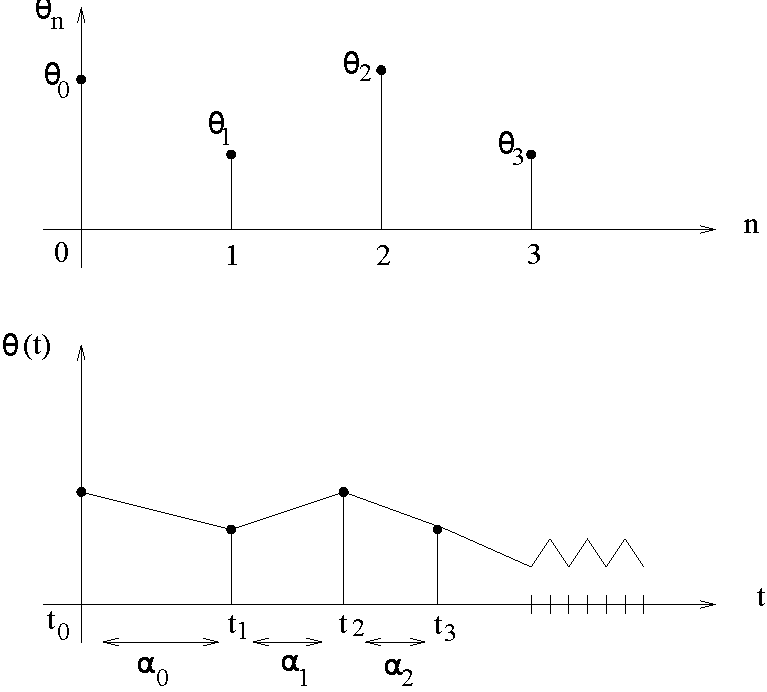
\includegraphics{figures/ch6_fig1a.pdf}}
\end{center}


Note that over a fixed $\Delta t$, the ``total gain'' is approximately
constant:
$$
\sum_{k\in K(t, \Delta t)} \alpha_k \simeq \Delta t\,,
$$
where $K(t,\Delta t) = \{k: t \le t_k < t+ \Delta t\}$.
Plugging in the update of Eq.~\ref{eq:stochastic_approx}, we have
$$
\theta(t+\Delta t) = \theta(t) + \sum_{\ttime\in K(t, \Delta t)} \alpha_\ttime [\safunc(X_\ttime)
+\omega_\ttime] \,.
$$
We now make two observations about the terms in the sum above:
\begin{enumerate}
\item
For large $t$, $\alpha_\ttime$ becomes small and the summation is over many
terms; thus the noise term is approximately ``averaged out'':
$\sum \alpha_\ttime \om_\ttime \to 0$.
\item
For small $\Delta t$, $X_\ttime$ is approximately constant over $K(t, \Delta t):
\safunc(X_\ttime) \simeq \safunc(\theta(t))$.
\end{enumerate}
We thus obtain:
$$
\theta(t+\Delta t) \simeq \theta(t) +\Delta t\cdot \safunc (\theta(t)),
$$
and rearranging gives,
$$
\frac{\theta(t+\Delta t) - \theta(t)}{\Delta t} \simeq  \safunc (\theta(t)).
$$
For $\Delta t \to 0$, this reduces to the ODE:
$$
\dot \theta(t) = \safunc(\theta(t)).
$$

We shall now discuss the convergence of the stochastic approximation iterates.  As $\ttime\to\infty$, we ``expect'' that the estimates
$\{\theta_\ttime\}$ will follow a trajectory of the ODE $\dot\theta=\safunc(\theta)$
(under the above time normalization). Thus, convergence can be expected to \textit{equilibrium points} (also termed \textit{stationary points} or \textit{fixed points}) of the ODE, that is, points $X^*$ that satisfy 
$\safunc(X^*) = 0$. We will also require the equilibrium to be {\em globally asymptotically stable}, as follows.
\begin{definition}
An ODE $\dot \theta(t) = \safunc(\theta(t))$ has a globally asymptotically stable equilibrium point $X^*$, if $\safunc(X^*) = 0$, and
for any $\theta_0$ we have that $\lim_{t \to \infty} \theta(t) = X^*$.
\end{definition}

We will mainly look at {\em $(A,B)$ well behaved} iterative
algorithms, where $B>0$ and $\discount\in(0,1)$, which have the
following properties:
\begin{enumerate}
\item Step size: we have (1) $\sum_\ttime
\alpha_\ttime
=\infty $, and (2)
$\sum_\ttime \alpha_\ttime^2=O(1)$,
\item Noise: $\E[\omega_\ttime(\state)|h_{\ttime-1}]=0$ and $|\omega_\ttime(\state)|\leq A + B\| X_\ttime\|^2$, for some norm $\| \cdot \|$ on $\mathbb{R}^d$, where
$h_{\ttime-1}$ is the history up to time $\ttime$,
\item $\safunc$ is Lipschitz continuous,
\item The ODE $\dot \theta(t) = \safunc(\theta(t))$ has a globally asymptotically stable equilibrium $X^*$,
\item The sequence $X_\ttime$ is bounded with probability 1.
\end{enumerate}
We now give a convergence result.

\begin{theorem}[Stochastic Approximation: ODE convergence]\ \\
\label{thm:stoch-approx-ODE}
 Let $X_\ttime$ be a sequence that is generated by a
$(A,B)$ well behaved iterative algorithm. Then $X_\ttime$
converges with probability $1$ to $X^*$.
\end{theorem}

% \uu{A Remark on Asynchronous Algorithms}:\quad
% When the stepsize is different for each component of $\theta$, the
% approximating ODE is more involved -- the relative rates should enter
% explicitly.
% Still, there exist specifc results that related
% the above ``synchronous'' ODE to the convergence of the
% asynchronous SA algorithm.


\begin{remark}
More generally, even if the ODE is not globally stable, $X_\ttime$ can be shown to converge
to an {\em invariant set} of the ODE (e.g., a limit cycle).
\end{remark}
% \begin{remark}
% Corresponding results exist for the asynchronous versions, under suitable
% assumptions on the relative gains.
% \end{remark}
\begin{remark}
A major assumption in the last result is the boundedness of $(X_\ttime)$.
In general this assumption has to be verified independently. However, there
exist several results that rely on further properties of $\safunc$ to deduce
boundedness, and hence convergence. One technique is to consider the function $\safunc_c(\theta) = \safunc(c \theta) / c$, $c\geq 1$. If $\safunc_c(\theta) \to \safunc_\infty(\theta)$ uniformly, one can consider the ODE with $\safunc_\infty$ replacing $\safunc$~\cite{borkar2009stochastic}. In particular, for a linear $\safunc$, we have that $\safunc_c = \safunc$, and this result shows that boundedness is guaranteed. We make this explicit in the following theorem.
\begin{theorem}[Stochastic Approximation: ODE convergence for linear systems]\ \\
\label{thm:stoch-approx-ODE-linear}
 Let $X_\ttime$ be a sequence that is generated by a
iterative algorithm that satisfies the first $4$ conditions of an $(A,B)$ well behaved algorithm, and $\safunc$ is linear in $\theta$. Then $X_\ttime$
converges with probability $1$ to $X^*$.
\end{theorem}
Another technique to guarantee boundedness
is to use the projected iterates:
$$
X_{\ttime+1} = \text{\it Proj}_\Gamma [X_\ttime+\alpha_\ttime((\safunc(X_\ttime)+\omega_\ttime) ]
$$
where $\text{\it Proj}_\Gamma$ is a projection onto some convex set $\Gamma$.
A simple example is when $\Gamma$ is a box, so that the components of $X$ are simply truncated at their minimal and maximal values. 
If $\Gamma$ is a bounded set then the estimated sequence $\{X_\ttime\}$ is guaranteed
to be bounded. However, in this case the corresponding ODE must account for the projection, and is $\dot \theta(t) = \safunc(\theta(t)) + \zeta$, where $\zeta$ is zero in the interior of $\Gamma$, and on the boundary of $\Gamma$, $\zeta$ is the infinitesimal change to $\theta$ required to keep it in $\Gamma$. In this case, to show convergence using Theorem \ref{thm:stoch-approx-ODE}, we must verify that $X^*$ is still a globally asymptotically stable equilibrium, that is, we must verify that the projection did not add a spurious stable point on the boundary of $\Gamma$. A thorough treatment of this idea is presented in \cite{kushner2003stochastic}.
\end{remark}

\section{Temporal Difference algorithms}
\label{sec:TD}
%In this lecture we will continue looking at model-free learning. In
%the previous lecture we presented: (1) $Q$-learning, which is an
%off-policy learning algorithm that learns the optimal $Q^*$
%function, (2) {\tt SARSA} which is an on-policy variant of
%$Q$-learning where we need to select actions, and (3) Monte-Carlo
%which is a model-free algorithm to learn the value function from
%episodes.

In this section we will look on temporal differences methods, which
work in an online fashion. We will start with $TD(0)$ which uses
only the most recent observations for the updates, and we will
continue with methods that allow for a longer look-ahead, and then
consider $TD(\lambda)$ which averages multiple look-ahead
estimations.

In general, temporal differences (TD) methods, learn directly from
experience, and therefore are model-free methods. Unlike Monte-Carlo
algorithms, they will use incomplete episodes for the updates, and
they are not restricted to episodic MDPs. The TD methods update
their estimates given the current observation and in that direction,
similar in spirit to $Q$-learning and SARSA.

\subsection{TD(0)}

Fix a policy $\policy\in \Pi_{SD}$, stationary and deterministic. The goal
is to learn the value function $\Value^\policy(\state)$ for every
$s\in S$. (The same goal as Monte-Carlo learning.) The TD algorithms
will maintain an estimate of the value function of the policy
$\policy$, i.e., maintain an estimate $\widehat{V}_\ttime(\state)$
for $\Value^\policy(\state)$. The TD algorithms will use their
estimates $\widehat{V}$ for the updates. This implies that unlike
Monte-Carlo, there will be an interaction between the estimates of
different states and at different times.

As a starting point, we can recall the {\em value iteration}
algorithm.
\[
V_{\ttime+1}(\state)=E^\policy[\reward(\state,\policy(\state))+\discount
V_\ttime(\state')]
\]
We have shown that value iteration converges, namely $V_\ttime
\rightarrow_{\ttime\rightarrow\infty} \Value^\policy$.

Assume we sample
$(\state_\ttime,\action_\ttime,\reward_\ttime,\state_{\ttime+1})$.
%Assume that $\policy\in SD$, namely a stationary deterministic policy.
Let $\widehat{V}_\ttime$ our estimation at time $\ttime$,
and we sample
$(\state_\ttime,\action_\ttime,\reward_\ttime,\state_{\ttime+1})$.
Then,
\[
E^\policy[\widehat{V}_\ttime(\state_\ttime)]=
E^\policy[\reward_\ttime+\discount
\widehat{V}_\ttime(\state_{\ttime+1})]=E^\policy[\reward(\state,\action)+\discount
\widehat{V}_\ttime(\state')|\state=\state_\ttime,a=\policy(\state)]
\]
%where $E^\policy [\widehat{V}_\ttime]=V_\ttime$.

The $TD(0)$ will do an update in this direction, namely,
$[\reward_\ttime+\discount \widehat{V}_\ttime(\state_{\ttime+1})]$.

\paragraph{$TD(0)$ Algorithm}

\begin{itemize}
\item \emph{Initialize:} $\widehat{V}(\state)$ arbitrarily.

\item At time $\ttime=0,1,\dots$:


-- Observe: $(\state_\ttime, \action_\ttime, \reward_\ttime,
\state_{\ttime+1})$.

-- Update:
%$(\state_\ttime,\action_\ttime,\reward_\ttime,\state_{\ttime+1})$:
\[
\widehat{V}(\state_\ttime)=\widehat{V}(\state_\ttime)+\alpha_\ttime(\state_\ttime,\action_\ttime)
\big[\reward_\ttime+\discount
\widehat{V}(\state_{\ttime+1})-\widehat{V}(\state_\ttime)\big]
\]
where $\alpha_\ttime(\state,\action)$ is the step size for
$(\state,\action)$ at time $\ttime$.
\end{itemize}

We define the {\em temporal difference} to be
\[
\Delta_\ttime =\reward_\ttime+\discount
\widehat{V}(\state_{\ttime+1})-\widehat{V}(\state_\ttime)
\]
The $TD(0)$ update becomes:
\[
\widehat{V}(\state_\ttime)=\widehat{V}(\state_\ttime)+\alpha_\ttime(\state_\ttime,\action_\ttime)\Delta_\ttime
\]


% [[YM: motivating example. Waze?!]]

We would like to compare the $TD(0)$ and the Monte-Carlo (MC)
algorithms. Here is a simple example with four states
$S=\{A,B,C,D\}$ where $\{C,D\}$ are terminal states and in $\{A,B\}$
there is one action (essentially, the policy selects a unique
action). Assume we observe eight episodes. One episode is
$(A,0,B,0,C)$, one episode $(B,0,C)$, and six episodes $(B,1,D)$. We
would like to estimate the value function of the non-terminal
states. For $V(B)$ both $TD(0)$ and $MC$ will give $6/8=0.75$. The
interesting question would be: what is the estimate for $A$? MC will
average only the trajectories that include $A$ and will get $0$
(only one trajectory which gives $0$ reward). The $TD(0)$ will
consider the value from $B$ as well, and will give an estimate of
$0.75$. (Assume that the $TD(0)$ continuously updates using the same
episodes until it converges.)

We would like to better understand the above example. For the above
example the empirical MDP will have a transition from $A$ to $B$,
with probability $1$ and reward $0$, from $B$ we will have a
transition to $C$ with probability $0.25$ and reward $0$ and a
transition to $D$ with probability $0.75$ and reward $1$. (See,
Figure~\ref{fig:L7-ML}.) The value of $A$ in the empirical model is
$0.75$. In this case the empirical model agrees with the $TD(0)$
estimate, we show that this holds in general.


\begin{figure}
  % Requires \usepackage{graphicx}
  \begin{centering}
  \includegraphics[width=0.5\textwidth]{figures/L7-ML}\\
  \caption{TD(0) vs. Monte-Carlo example}\label{fig:L7-ML}
  \end{centering}
\end{figure}


\paragraph{Maximum Likelihood model}\footnote{YM: repeat} Recall that the empirical model, which is also the
maximum likelihood model, of a sample be define as follows. Let
$n(\state,\action)$ be the number of times $(\state,\action)$
appears in the sample. Given a sample
$(\state_\ttime,\action_\ttime,\reward_\ttime,\state_{\ttime+1})$
for $1\leq t\leq T$, we define the empirical model as follows. The
rewards $\widehat{\reward}(\state,\action)$ are the average rewards
of $(\state,\action)$, i.e.,
$\widehat{\reward}(\state,\action)=\frac{1}{n(\state,\action)}\sum_{\ttime:\state_\ttime=\state,\action_\ttime=\action}\reward_\ttime$
and
$\widehat{\transitionprob}(\state'|\state,\action)=\frac{n(\state,\action,\state')}{n(\state,\action)}$,
where $n(\state,\action,\state')$ is the number of samples that have
$\state_{\ttime+1}=\state'$ when $\state_\ttime=\state$ and
$\action_\ttime =\action$.

The following theorem states that the value of the policy $\policy$ on the
empirical model is identical to that of $TD(0)$ (running on the
sample until convergence, namely, continuously sampling uniformly
$t\in[1,T]$ and using $(\state_\ttime,
\action_r,\reward_\ttime,\state_{\ttime+1})$ for the $TD(0)$
update).

\begin{theorem}
Let $\Value^\policy_{TD}$ be the estimated value function of
$\policy$ when we run $TD(0)$ until convergence. Let
$\Value^\policy_{EM}$ be the value function of $\policy$ on the
empirical model. Then, $\Value^\policy_{TD}=\Value^\policy_{EM}$.
\end{theorem}

\begin{proof}[Proof sketch]
The update of $TD(0)$ is
$\widehat{V}(\state_\ttime)=\widehat{V}(\state_\ttime)+\alpha_\ttime(\state_\ttime,\action_\ttime)\Delta_\ttime$,
where $\Delta_\ttime=\reward_\ttime+\discount
\widehat{V}(\state_{\ttime+1})-\widehat{V}(\state_\ttime)$. At
convergence we have $E[\Delta_\ttime]=0$ and hence,
\[
\widehat{V}(\state)=\frac{1}{n(\state,\action)}\sum_{\state_{\ttime+1}:\state_\ttime=\state,\action_\ttime=\action}
\reward_\ttime+\discount
\widehat{V}(\state_{\ttime+1})=\widehat{\reward}(\state,\action)+\discount
E_{\state'\sim
\widehat{\transitionprob}(\cdot|\state,\action)}[\widehat{V}(\state')]
\]
where $\action=\policy(\state)$.
\end{proof}

It is worth to compare the above theorem to the case of Monte Carlo
(Theorem~\ref{thm:MC-ML}). Here we are using the entire sample, and
we have the same ML model for any state $\state$. In the Monte-Carlo
case we used a reduced sample, which depends on the state $\state$
and therefore we have a different ML model for each state, based on
its reduced sample.

\paragraph{Convergence:} The proof of the convergence of $TD(0)$ is very
similar to that of $Q$-learning. We will show that $TD(0)$ is an
instance of the stochastic approximation algorithm, as presented in
previously in Section~\ref{sec:stochastic-approximation}, and the
convergence proof will follow from this.
%We will first state it.

\begin{theorem}[Convergence $TD(0)$]
\label{thm:TD0-conrg} If the step size has the properties that for
every $(\state,\action)$ we have $\sum_\ttime
\alpha_\ttime(\state,\action)=\infty $ and $\sum_\ttime
\alpha_\ttime^2(\state,\action)=O(1)$, then $\widehat{V}$ converges
to $\Value^\policy$, with probability $1$.
\end{theorem}

We will show the convergence using the general theorem for
stochastic approximation iterative algorithm
(Theorem~\ref{thm:stoch-approx}).

We first define a linear operator $H$ for the policy $\policy$,
\[
(Hv)(\state)=\reward(\state,\policy(\state))+\discount\sum_{\state'}\transitionprob(\state'|\state,\policy(\state))v(\state')
\]
Note that $H$ is the operator $T^\policy$ we define in
Section~\ref{ss:DP_op}.

As we saw before, the operator $H$ is a $\discount$-contracting, namely,
operator
\begin{align*}
\|Hv_1-Hv_2\|_\infty &= \discount \max_{s} |
\sum_{\state'}\transitionprob(\state'|\state,\policy(\state))(v_1(\state')-v_2(\state'))|\\
&\leq \discount\max_{\state'} |v_1(\state')-v_2(\state')|\\
&\leq \discount \|v_1-v_2\|_\infty
\end{align*}
%Therefore $H$ is $\discount$-contracting.

We now would like to re-write the $TD(0)$ update to be a stochastic
approximation iterative algorithm. The $TD(0)$ update is,
\[
V_{\ttime+1}(\state_\ttime)=(1-\alpha_\ttime)V_\ttime(\state_\ttime)+\alpha_\ttime
\Phi_\ttime
\]
where $\Phi_\ttime=\reward_\ttime+\discount
V_\ttime(\state_{\ttime+1})$. We would like to consider the expected
value of $\Phi_\ttime$. Clearly,
$E[\reward_\ttime]=\reward(\state_\ttime,\policy(\state_\ttime))$
and $\state_{\ttime+1} \sim \transitionprob(\cdot |\state_\ttime,\action_\ttime)$.
This implies that $E[\Phi_\ttime]=(HV_\ttime)(\state_\ttime)$.
Therefore, we can define the noise term $\omega_\ttime$ as follows,
\[
\omega_\ttime(\state_\ttime)=[\reward_\ttime+\discount
V_\ttime(\state_{\ttime+1})]-(HV_\ttime)(\state_\ttime)\;,
\]
and have $E[\omega_\ttime]=0$. We can bound $|\omega_\ttime|\leq
V_{max}=\frac{R_{max}}{1-\discount}$, since the value function is
bounded by $V_{max}$.

Returning to $TD(0)$, we can write
\[
V_{\ttime+1}(\state_\ttime)=(1-\alpha_\ttime)V_\ttime(\state_\ttime)+\alpha_\ttime
[(HV_\ttime)(\state_\ttime)+\omega_\ttime(\state_\ttime)]
\]
The requirement of the step size appears in the statement of the
theorem (and so holds). The noise $\omega_\ttime$ has both
$E[\omega_\ttime]=0$ and $|\omega_\ttime|\leq V_{max}$. The
operator $H$ is $\discount$-contracting with a fix-point $\Value^\policy$.
Therefore, using Theorem~\ref{thm:stoch-approx}, we established
Theorem~\ref{thm:TD0-conrg}.

\paragraph{Comparing various algorithms:}\footnote{YM: needed? I think it is from Sutton}
When we compare $TD(0)$, to $MC$ and both to  Dynamic Programming
(DP) we can view it as different ways of computing the value
function.
\begin{itemize}
\item[MC] We have $\Value^\policy(\state)=E[R_\ttime|\state_\ttime=\state]$. In MC we observe the
return, $R_\ttime$, of episodes, and their mean is what we like to
estimate.
\item [$TD(0)$]  We have $\Value^\policy(\state)=E[\reward_\ttime+\discount \Value^\policy(\state_{\ttime+1})|\state_\ttime=\state]$. In $TD(0)$ we observe samples of
$\reward_\ttime$, we use our estimate for
$\Value^\policy(\state_{\ttime+1})$ and the expectation is what we
like to estimate (assuming our estimates converge).
\item
[DP]
 We have $\Value^\policy(\state)=\sum_{\action}\policy(\action|\state)[\reward(\state,\action)+\discount \sum_{\state'}\transitionprob(\state'|\state,\action)\Value^\policy(\state')]$. In DP we
 have the entire model, and use it to compute expectations.
\end{itemize}

We can see the difference between $TD(0)$ and $MC$ in the Markov
Chain in Figure~\ref{fig:L7-TD-MC}. To get an approximation of state
$\state_2$, i.e., $|\widehat{V}(\state_2)-\frac{1}{2}|\approx
\varepsilon$. The Monte-Carlo will require $O(1/(\beta
\varepsilon^2))$ episodes (out of which only $O(1/\varepsilon^2)$
start at $\state_2$) and the $TD(0)$ will require only
$O(1/\varepsilon^2+1/\beta)$ since the estimate of $\state_3$ will
converge after $1/\varepsilon^2$ episodes which start from
$\state_1$.

\begin{figure}
  % Requires \usepackage{graphicx}
  \begin{centering}
  \includegraphics[width=0.5\textwidth]{figures/L7-TD-MC}\\
  \caption{Markov Reward Chain}\label{fig:L7-TD-MC}
  \end{centering}
\end{figure}

\subsection{Q-learning: Markov Decision Process}


We now extend the $\QValue$-learning algorithm from DDP to MDP. The main
difference is that now we will need to average multiple observations
to converge to the value of $\QValue^*$. For this we introduce
learning rates for each state-action pair, $\alpha_\ttime(\state,\action)$. We allow the
learning rate to depend both on the state $\state$, action $\action$
and time $\ttime$. For example $\alpha_\ttime(\state,\action)=1/n$
where $n$ is the number of times we updated $(\state,\action)$ up to
time $\ttime$. The following is the definition of the algorithm.

\paragraph{The $\QValue$-learning algorithm:}

\begin{itemize}
\item {\em Initialize:} Set $ Q_0(\state,\action)=0$, for all $\state$, $\action$.

\item At time $\ttime=0,1,\dots$:

-- Observe: $(\state_\ttime, \action_\ttime, \reward_\ttime,
\state_{\ttime}')$.
% $s\leftarrow \state_n$, $a \leftarrow \action_n$, $r\leftarrow \reward_n$, $s'\leftarrow \state_{n+1}$.

-- Update: %$\widehat{\QValue}(\state_\ttime,\action_\ttime)$:
\begin{align*}
 Q_{\ttime+1}(\state_\ttime,\action_\ttime) & :=
 Q_\ttime (\state_\ttime,\action_\ttime) + \alpha_\ttime(\state_\ttime,\action_\ttime)  [\reward_\ttime +
\discount \max_{\action'} Q_\ttime (\state_{\ttime}', \action')
-Q_\ttime (\state_\ttime,\action_\ttime)]
\end{align*}
\end{itemize}


It is worth to try and gain some intuition regarding the $Q$
learning algorithm. Let $\Gamma_\ttime= \reward_\ttime + \discount
\max_{\action'} Q_\ttime (\state_{\ttime}', \action')-Q_\ttime
(\state_\ttime,\action_\ttime)$.
%
For simplicity assume we already converged,
%
%The basic intuition is that if
$Q_\ttime=\QValue^*$. Then we have that $\E[\Gamma_\ttime]=0$ and (on
average) we maintain that $Q_\ttime=\QValue^*$.
%
Clearly we do not want to assume that we converge, since this is the
entire goal of the algorithm.
%
The main challenge in showing the convergence is that in the updates
we use $Q_\ttime$ rather than $\QValue^*$. We also need to handle the
stochastic nature of the updates, where there are both stochastic
rewards and stochastic next state.

The next theorem states the main convergence property of
$\QValue$-learning.
\begin{theorem}[$\QValue$-learning convergence]\ \\
\label{thm:Q-learning} Assume every state-action pair
$(\state,\action)$ occurs infinitely often, and the step size
$\alpha_\ttime(\state,\action)$ has the properties: (1) $\sum_\ttime
\alpha_\ttime(\state,\action)
I(\state_\ttime=\state,\action_\ttime=\action)=\infty $, and (2)
$\sum_\ttime
\alpha_\ttime^2(\state,\action) I(\state_\ttime=\state,\action_\ttime=\action)=O(1)$,\\
Then, $Q_\ttime$ converges with probability $1$ to $\QValue^*$
\end{theorem}

Note that the statement of the theorem has two requirements. The
first is that every state-action pair occurs infinitely often.
This is clearly required for convergence (per state-action). Since
$\QValue$-learning is an off-policy, it has no influence on the sequence
of state-action it observes, and therefore we have to make this
assumption. The second requirement is two properties regarding the
learning rates $\alpha$. The first states that the learning rates
are large enough that we can (potentially) reach a value. The
second states that the learning rates are sufficiently small (sum of
squares finite) so that we will be able to converge locally.

We will show the convergence proof by introducing a general technique
of stochastic approximation. (We will not give the details of the
proof of stochastic approximation, but will only outline the main
building blocks and the methodology.) Given the stochastic
approximation convergence theorem, we later show how to use it to
derive the convergence of the $\QValue$-learning algorithm.




\subsection{$\QValue$-learning as a stochastic approximation}

After we introduced the stochastic approximation algorithms, and
their convergence theorem, we show that the $\QValue$-learning algorithm
is a stochastic approximation algorithm, and thus converges.
%
To show that $\QValue$-learning algorithm is a stochastic approximation
algorithm we need to introduce an operator $H$ and the noise
$\omega$.

We first define the operator $H$,
\[
(Hq)(\state,\action)=\sum_{\state'}p(\state'|\state,\action)
[\reward(\state,\action) + \discount \max_{\action'} q (\state',
\action')]
\]
The contraction of $H$ is established as follows,
\begin{align*}
\|Hq_1-Hq_2\|_\infty &= \discount \max_{\state,\action}
|\sum_{\state'} p(\state'|\state,\action)
[\max_{b_1} q_1(\state',b_1)-\max_{b_2} q_2(\state',b_2)|\\
&\leq \discount \max_{\state,\action}\max_{b,\state'} |q_1(\state',b)-q_2(\state',b)|\\
&\leq \discount \|q_1-q_2\|_\infty\;.
\end{align*}


In this section we re-write the $\QValue$-learning algorithm to follow the
iterative stochastic approximation algorithms, so that we will be
able to apply Theorem~\ref{thm:stoch-approx}.

Recall that,
\begin{align*}
 Q_{\ttime+1}(\state_\ttime,\action_\ttime) & :=   (1-\alpha_\ttime(\state_\ttime,\action_\ttime) ) Q_\ttime (\state_\ttime,\action_\ttime) + \alpha_\ttime(\state_\ttime,\action_\ttime)  [\reward_\ttime +
\discount \max_{\action'} Q_\ttime (\state_{\ttime}',
\action')]
\end{align*}
Let $\Phi_\ttime=\reward_\ttime + \discount \max_{\action'} Q_\ttime
(\state_{\ttime+1}, \action')$. This implies that $\E[\Phi_\ttime]=
(HQ_\ttime)(\state_\ttime,\action_\ttime)$. We can define the noise
term as
$\omega_\ttime(\state_\ttime,\action_\ttime)=\Phi_\ttime-(HQ_\ttime)(\state_\ttime,\action_\ttime)$
and have $\E[\omega_\ttime(\state_\ttime,\action_\ttime)]=0$. In
addition $|\omega_\ttime(\state_\ttime,\action_\ttime)|\leq \Vmax=
\frac{R_{max}}{1-\discount}$.

We can now rewrite the $\QValue$-learning, as follows,
\begin{align*}
 Q_{\ttime+1}(\state_\ttime,\action_\ttime) & :=   (1-\alpha_\ttime(\state_\ttime,\action_\ttime) ) Q_\ttime (\state_\ttime,\action_\ttime) + \alpha_\ttime(\state_\ttime,\action_\ttime)
 [(HQ_\ttime)(\state_\ttime,\action_\ttime)+\omega_\ttime(\state_\ttime,\action_\ttime)]
\end{align*}

In order to apply Theorem~\ref{thm:stoch-approx}, we have the
properties of the noise $\omega_\ttime$, and of the contraction of
$H$. Therefore, we can derive Theorem~\ref{thm:Q-learning}, since
the step size requirement is part of the theorem.

\subsection{Step size}

The step size has important implication for the convergence of the
Q-learning algorithm, and more importantly, on the rate convergence.
For the convergence, we need for the step size to have two
properties. The first is that sum diverges, i.e., $\sum_\ttime
\alpha_\ttime(\state,\action)
I(\state_\ttime=\state,\action_\ttime=\action)=\infty $, which
intuitively implies that we can potentially reach any value. This is
important, since we might have errors on the way, and this
guarantees that the step sizes are large enough to possibly
correct any error. (It does not guarantee that it will correct the
errors, only that the step size is large enough to allow for it.)

The second requirement from the step size is that the sum of squares
converges, i.e., $\sum_\ttime \alpha_\ttime^2(\state,\action)
I(\state_\ttime=\state,\action_\ttime=\action)=O(1)$. This
requirement is that the step size are not too large. It will
guarantee that once we are close to the correct value, the step size
will be small enough that we actually converge, and not bounce
around.

Consider the following experiment. Suppose from some time $\tau$
we update using only $\QValue^*$, then we clearly would like to converge.
For simplicity assume there is no noise, i.e., $\omega_\ttime=0$ for
$\ttime\geq\tau$ and assume a single state., i.e., $\QValue^*\in \Reals$.
For the update we have that $Q_{\ttime+1}=(1-\alpha_\ttime)Q_\ttime
+\alpha_\ttime \QValue^*$ or equivalently, $Q_{\ttime+1}=\beta
Q_\tau+(1-\beta)\QValue^*$, where $\beta=
\prod_{i=\tau}^\ttime(1-\alpha_i)$. We like to have that $\beta$
converges to $0$ and a sufficient condition is that
$\sum_i\alpha_i=\infty$.
%
%Next, assume that there is bounded noise, i.e. $\E[w_\ttime]=0$ and
%$|w_\ttime|\leq 1$. Now we have
%$Q_{\ttime+1}=(1-\alpha_\ttime)Q_\ttime +\alpha_\ttime
%(\QValue^*+w_\ttime)$, or equivalently, $Q_{\ttime+1}=\beta_\ttime
%Q_\tau+(1-\beta_\ttime)\QValue^*+W$, where $\beta_\ttime=
%\prod_{i=\tau}^\ttime(1-\alpha_i)$ and $W=\sum_{i=\tau}^\ttime
%\alpha_\ttime\beta_{\ttime-1}w_\ttime$. As before, we have that
%$\beta_\ttime$ approaches $1$. In addition we like $W$ to approach
%$0$. We can now use the McDiarmid inequality
%(Lemma~\ref{lemma:McDiarmid}). Fix an accuracy $\varepsilon>0$ and
%confidence $\delta>0$. Since $\sum_i \alpha_i =O(1)$, there is an
%index $\tau'$ such that $\sum_{i>\tau'} \alpha_i <
%\varepsilon^2/(\log 1/\delta)$. This implies that after $\tau'$ the
%value of $W$ will be at most $\varepsilon$.
%
%This will hold since $\alpha_\tau$ approaches $0$ and in addition
%$\sum_{i=\tau} \alpha_i^2 $ approaches $0$. [YM:need to complete]
%
% The large enough step size will
%guarantee that we will reach $\QValue^*$ neighborhood, regardless of where
%we started.
The small enough step size will guarantee that we will converge even
when the noise is not zero (but bounded).

Many times step size is simply a function of the number of visits
to $(\state,\action)$, which we denote by $n(\state,\action)$, and
this is widely used in practice. Two leading examples are:
\begin{enumerate}
\item
{\em Linear step size:}
$\alpha_\ttime(\state,\action)=1/n(\state,\action)$. We have that
$\sum_{n=1}^N 1/n=\ln(N)$ and therefore $\sum_{n=1}^\infty
1/n=\infty$. Also, $\sum_{n=1}^\infty 1/n^2=\policy^2/6=O(1)$
\item
{\em Polynomial step size}: For $\theta\in(1/2,1)$ we have
$\alpha_\ttime(\state,\action)=1/(n(\state,\action))^\theta$. We
have that $\sum_{n=1}^N 1/n^\theta\approx
(1-\theta)^{-1}N^{1-\theta}$ and therefore $\sum_{n=1}^\infty
1/n^\theta=\infty$. Also, $\sum_{n=1}^\infty 1/n^{2\theta} \leq
\frac{1}{2\theta-1}$, since $2\theta>1$.
\end{enumerate}

The linear step size, although many times popular in practice, might
lead to slow converges. Here is a simple example. We have a single
state $\state$ and single action $\action$ and
$\reward(\state,\action)=0$. However, suppose we start with
$Q_0(\state,\action)=1$. We will analyze the convergence with the
linear step size. Our update is,
\[
Q_\ttime =
(1-\frac{1}{\ttime})Q_{\ttime-1}+\frac{1}{\ttime}[0+\discount
Q_{\ttime-1}]=(1-\frac{1-\discount}{\ttime})Q_{\ttime-1}
\]
When we solve the recursion we get that
$Q_\ttime=\Theta(1/\ttime^{1-\discount})$.\footnote{$Q_\ttime=\prod_{i=1}^\ttime (1-(1-\discount)/i)\approx
\prod_{i=1}^\ttime e^{-(1-\discount)/i}=e^{-\sum_{i=1}^\ttime
(1-\discount)/i }\approx e^{-(1-\discount)\ln
t}=t^{-(1-\discount)}$. }
%
This implies that for $t\leq  (1/\varepsilon)^{1/(1-\discount)}$ we
have $Q_\ttime \geq \varepsilon$.

In contrast, if we use a polynomial step size, we have,
\[
Q_\ttime =
(1-\frac{1}{t^\theta})Q_{\ttime-1}+\frac{1}{t^\theta}[0+\discount
Q_{\ttime-1}]=(1-\frac{1-\discount}{t^\theta})Q_{\ttime-1}
\]
When we solve the recursion we get that
$Q_\ttime=\Theta(e^{-(1-\discount)t^{1-\theta}})$. This implies that
for $t\geq \frac{1}{1-\discount}\log^{1/(1-\theta)} (1/\varepsilon)$
we have $Q_\ttime \leq \varepsilon$. This is a poly-logarithmic
dependency on $\varepsilon$, which is much better. Also, note that
$\theta$ is under our control, and we can set for example
$\theta=2/3$. Note that unlike $\theta$, the setting of the discount
factor $\discount$ has a huge influence on the objective function
and the effective horizon.

\subsection{SARSA: on-policy $\QValue$-learning}

The Q-learning algorithm that we presented is an off-policy
algorithm. This implies that it has no control over the action
selection. The benefit is that it does not face the exploration
exploitation trade-off and its only goal is to approximate the
optimal $\QValue$ function.

In this section we would like to extend the $\QValue$-learning algorithm
to an on-policy setting. This will first of all involve selecting
the actions by the algorithm. Given that the actions are set by the
algorithm, we can consider the return of the algorithm. We would
like the return of the algorithm to converge to the optimal return.


%We would like to have an on-policy variant of $\QValue$-learning, which
The specific algorithm that we present is called SARSA. The name
comes from the fact that the feedback we observe
$(\state_\ttime,\action_\ttime,\reward_\ttime,\state_{\ttime+1},\action_{\ttime+1})$,
ignoring the subscripts we have SARSA. Note that since it is an
on-policy algorithm, the actions are actually under the control of
the algorithm, and we would need to specify how to select them.

When designing the algorithm we need to think of two contradicting
objectives in selecting the actions. The first is the need to
explore, perform each action infinitely often. This implies that we
need, for each state $\state$ and action $\action$, to have that $\sum_\ttime
\policy_\ttime(\action|\state)=\infty$. Then by the Borel-Cantelli
lemma we have with probability $1$ an infinite number of times that
we select action $\action$ in state $\state$ (actually, we need
independence of the events, or at least a Martingale property, which
holds in our case). On the other hand we would like not only our
estimates to converge, as done in $\QValue$-learning, but also the return
to be near optimal. For this we need the action selection to
converge to being greedy with respect to the $\QValue$ function.

\paragraph{The SARSA algorithm}\ \\


\begin{itemize}
\item {\em Initialize:} Set $ Q_0(\state,\action)=0$, for all $\state$, $\action$.

\item At time $\ttime=0,1,\dots$:

-- Observe
$(\state_\ttime,\action_\ttime,\reward_\ttime,\state_{\ttime+1})$.
% $s\leftarrow \state_n$, $a \leftarrow \action_n$, $r\leftarrow \reward_n$, $s'\leftarrow \state_{n+1}$.

--Select $\action_{\ttime+1}=\policy(\state_{\ttime+1};Q_\ttime)$.

-- Update %$\widehat{\QValue}(\state_\ttime,\action_\ttime)$:
\begin{align*}
 Q_{\ttime+1}(\state_\ttime,\action_\ttime) & :=   Q_\ttime (\state_\ttime,\action_\ttime) + \alpha_\ttime(\state_\ttime,\action_\ttime)  [\reward_\ttime +
\discount  Q_\ttime (\state_{\ttime+1}, a_{\ttime+1}) -Q_\ttime
(\state_\ttime,\action_\ttime)]
\end{align*}
\end{itemize}
Note that SARSA selects an action $\action_{\ttime+1}$ for state
$\state_{\ttime+1}$, dependent on the values of $Q_\ttime$ and not
$Q_{\ttime+1}$. The update of $Q_\ttime$ is done only after we
selected action $\action_{\ttime+1}$ (which is performed at time
$\ttime+1$).

\paragraph{Selecting the action:}
As we discussed before, one of the main tasks of an on-policy
algorithm is to select the actions. It would be natural to select
the action is state $\state_\ttime$ as a function of our current
approximation $Q_\ttime$ of the optimal $\QValue$ function.

Given a state $\state$ and a $\QValue$ function $Q$, we first define the
greedy action in state $\state$ according to $Q$ as
\[
\bar{\action}=\arg\max_\action Q(\state,\action)
\]
The first idea might be to simply select the greedy action
$\bar{\action}$, however this might be devastating. The main issue
is that we might be avoiding exploration. Some actions might look better
due to errors, and we will continue to execute them and not gain any
information about alternative actions.


For a concrete example, assume we initialize $Q_0$ to be $0$.
Consider an MDP with a single state and two actions $\action_1$ and
$\action_2$. The reward of action $\action_1$ and $\action_2$ are a
Bernoulli random variables with parameters $1/3$ and $3/4$,
respectively. If we execute action $\action_1$ first and get a
reward of $1$, then we have $Q_1(\state,\action_1)>0$ and
$Q_1(\state,\action_2)=0$. If we select the greedy action, we will
\emph{always} select action $\action_1$. We will both be sub-optimal
in the return and never explore $\action_2$ which will result that
we will not converge to $\QValue^*$. For this reason we would not select
deterministically the greedy action.


In the following we will present two simple ways to select the
action by $\policy(\state;Q)$ stochastically. Both ways will give
all actions a non-zero probability, and thus guarantee exploration.
%\[
%\bar{\action}=\arg\max Q(\state,\action)
%\]

The \emph{ $\varepsilon_n$-greedy}, has as a parameter a sequence of
$\varepsilon_n$ and selects the actions as follows. Let
$n_\ttime(\state)$ be the number of times state $\state$ was visited
up to time $\ttime$. At time $\ttime$ in state $\state$ policy
$\varepsilon_n$-greedy (1) with probability $1-\varepsilon_n$ sets
$\policy(\state;Q)=\bar{\action}$ where $n=n_\ttime(\state)$, and
(2) with probability $\varepsilon_n/|\Actions|$, selects
$\policy(\state;Q)=\action$, for each $\action \in \Actions$. Common
values for $\varepsilon_n$ are linear, $\varepsilon_\ttime=1/n$, or
polynomial, $\varepsilon_\ttime=1/n^\theta$ for $\theta\in(0.5,1)$.

The {\em soft-max}, has as a parameter a sequence of
$\beta_\ttime\geq 0$ and selects $\policy(\state;Q)=\action$, for
each $\action \in \Actions$, with probability $\frac{e^{\beta_\ttime
Q(\state,\action)}}{\sum_{\action'\in \Actions}e^{\beta_\ttime
Q(\state,\action')}}$. Note that for $\beta_\ttime=0$ we get the
uniform distribution and for $\beta_\ttime\rightarrow \infty$ we get
the maximum. We would like the schedule of the $\beta_\ttime$ to go
to infinity (become greedy) but need it to be slow enough (so that
each action appears infinitely often).

\begin{advanced}
\paragraph{SARSA convergence:}
Convergence of the $Q_\ttime$ to $\QValue^*$ would follow immediately from
the basic properties of the $\QValue$-learning, we just need to guarantee
that we explore each action infinitely often. (This would follow
since any $\varepsilon$-greedy policy is aperiodic and irreducible,
the steady state of the resulting Markov has a non-zero probability
at each state, so each state would be visited infinitely often.)
Then, the result will follow immediately from the convergence of
$\QValue$-learning.

The convergence of the return of SARSA to that of $\QValue^*$ is more
delicate. Recall that we do not have such a claim about
$\QValue$-learning, since it is an off-policy method. For the convergence
of the return we need to make our policy `greedy enough', in the
sense that it has enough exploration, but guarantees a high return
through the greedy actions. The following lemma shows that if we
have a strategy which is greedy with respect to a near optimal $Q$
function, then the policy is near optimal.

\begin{lemma}
\label{lemma:Q-greedy-policy}
%
Let $Q$ such that $\| Q-\QValue^*\|_\infty \leq \Delta$, and $\policy$ the
greedy policy w.r.t. $Q$, i.e., $\policy(\state)\in \arg\max_\action
Q(\state,\action)$. Then,
$\Value^*(\state)-\Value^\policy(\state)\leq
\frac{2\Delta}{1-\discount}$.
\end{lemma}
\begin{proof}
First, we show that for any state $\state$ we have
$\Value^*(\state)-\QValue^*(\state,\policy(\state))\leq 2\Delta$. Since
$\| Q-\QValue^*\|_\infty \leq \Delta$ we have
$|\QValue^*(\state,\policy(\state))-Q(\state,\policy(\state))|\leq \Delta$
and $|\QValue^*(\state,\action^*)-Q(\state,\action^*)|\leq \Delta$, where
$\action^*$ is the optimal action in state $\state$. This implies that
%
$\QValue^*(\state,\action^*)-\QValue^*(\state,\policy(\state))\leq
Q(\state,\action^*)-Q(\state,\policy(\state))+2\Delta$.
%
Since policy $\policy$ is greedy w.r.t. $Q$ we have
$Q(\state,\policy(\state))\geq Q(\state,\action^*)$, and hence
$\Value^*(\state)-\QValue^*(\state,\policy(\state))=\QValue^*(\state,\action^*)-\QValue^*(\state,\policy(\state))\leq
2\Delta$.


Next,
$$\Value^*(\state)=\QValue^*(\state,\action^*)\leq \QValue^*(\state,\policy(\state))+2\Delta = \E[\reward_0]+\discount
\E[\Value^*(\state_1)]+2\Delta,$$ where
$\reward_0=\E[R(\state,\policy(\state))]$ and $\state_1$ is the state
reached when doing action $\policy(\state)$ in state $\state$. As we
role out to time $\ttime$ we have,
\[
\Value^*(\state)\leq \E[\sum_{i=0}^{\ttime-1} \discount^i
\reward_i]+\discount^\ttime
\E[\Value^*(\state_\ttime)]+\sum_{i=1}^\ttime 2\Delta\discount^i
\]
where $\reward_i$ is the reward in time $i$ in state $\state_i$,
$\state_{i+1}$ is the state reached when doing action
$\policy(\state_i)$ in state $\state_i$, and we start with
$\state_0=\state$.
%
This implies that in the limit we have
\[
\Value^*(\state)\leq \Value^\policy(\state)+\frac{
2\Delta}{1-\discount},
\]
since $\Value^\policy(\state)=\E[\sum_{i=0}^{\infty} \discount^i
\reward_i]$.
\end{proof}

The above lemma uses the greedy policy, but as we discussed before,
we would like to add exploration. We would like to claim that if
$\varepsilon$ is small, then the difference in return between the
greedy policy and the $\varepsilon$-greedy policy would be small. We
will show a more general result, showing that for any policy, if we
add a perturbation of $\varepsilon$ to the action selection, then
the effect on the expected return is at most $O(\varepsilon)$.

Fix a policy $\policy$ and let $\policy_\varepsilon$ be a policy
such that for any state $\state$ we have that
$\|\policy(\cdot|\state)-\policy_\varepsilon(\cdot|\state)\|_1\leq\varepsilon$.
Namely, there is a policy $\rho(\action|\state)$ such that
$\policy_\varepsilon(\action|\state)=(1-\varepsilon)\policy(\action|\state)+\varepsilon
\rho(\action|\state)$. Hence, at any state, with probability at
least $1-\varepsilon$ policy $\policy_\varepsilon$ and policy
$\policy$ use the same action selection.

\begin{lemma}
\label{lemma:epsilon-greedy}
%
Fix $\policy_\varepsilon$ and policy $\policy$ such that for any
state $\state$ we have that
$\|\policy(\cdot|\state)-\policy_\varepsilon(\cdot|\state)\|_1\leq\varepsilon$.
Then, for any state $\state$ we have
\[
|\Value^{\policy_\varepsilon}(\state)-\Value^\policy(\state)|\leq
\frac{\varepsilon\discount}{(1-\discount)(1-\discount(1-\varepsilon))}\leq \frac{\varepsilon}{(1-\discount)^2}
\]
%For $\varepsilon\leq 1/2$ we have $|\Value^{\policy_\varepsilon}(\state)-\Value^\policy(\state)|\leq 2\varepsilon\Vmax$
\end{lemma}

\begin{proof}
Let $\reward_\ttime$ be the reward of policy $\policy$ at time
$\ttime$. By definition
$\Value^\policy(\state)=\E[\sum_{\ttime=0}^\infty
\discount^\ttime\reward_\ttime]$. The probability that policy
$\policy_\varepsilon$ never deviated from $\pi$ until time $\ttime$
is $(1-\varepsilon)^\ttime$. Therefore we can lower bound the
expected reward of policy $\policy_\varepsilon$ by
$\Value^{\policy_\varepsilon}(\state)\geq \E[\sum_{\ttime=0}^\infty
(1-\varepsilon)^\ttime\discount^\ttime\reward_\ttime]$.

Consider the difference between the expected returns,
\[
\Value^\policy(\state)- \Value^{\policy_\varepsilon}(\state) \leq
\E[\sum_{\ttime=0}^\infty \discount^\ttime\reward_\ttime] -
\E[\sum_{\ttime=0}^\infty
(1-\varepsilon)^\ttime\discount^\ttime\reward_\ttime]
\]
Since the rewards are bounded, namely, $\reward_\ttime\in[0,1]$, the
difference is maximized if we set all the rewards to $1$, and have
\[
\Value^\policy(\state)- \Value^{\policy_\varepsilon}(\state) \leq
\sum_{\ttime=0}^\infty \discount^\ttime - \sum_{\ttime=0}^\infty
(1-\varepsilon)^\ttime\discount^\ttime=
\frac{1}{1-\discount}-\frac{1}{1-\discount(1-\varepsilon)}=\frac{\varepsilon\discount}{(1-\discount)(1-\discount(1-\varepsilon))}
\]
% Since $\Vmax=\frac{1}{1-\discount}$ and $\discount< 1$, for
% $\varepsilon\leq 1/2$ we have
% \[
% \Value^\policy(\state)- \Value^{\policy_\varepsilon}(\state) \leq
% 2\varepsilon\Vmax
% \]
\end{proof}

We can now combine the results and claim that SARSA with
$\varepsilon$-greedy converges to the optimal policy. We will need
that $\varepsilon_n$-greedy uses a sequence of $\varepsilon_n$ such
that $\varepsilon_n$ converges to zero as $n$ increases. Call such a
policy \emph{monotone $\varepsilon_n$-greedy policy}.

\begin{theorem}
For any $\lambda>0$ there is a time $\tau$ such that at any time
$\ttime>\tau$ the algorithm SARSA, using a monotone
$\varepsilon_n$-greedy policy, plays a $\lambda$-optimal policy.
\end{theorem}

\begin{proof}
Consider the sequence $\varepsilon_n$. Since it converges to zero, there exists a value $N$ such that for any $n\geq N$ we have $\varepsilon_n\leq 0.25\lambda(1-\discount)^2$.

Since we are guaranteed that each state action is sampled infinitely
often, there is a time $\tau_1$ such that each state is sampled at
least $N$ times.

Since $Q_\ttime$ converges to $\QValue^*$, there is a time $\tau_2$ such that for any $\ttime\geq \tau_2$ we have $\|Q_\ttime-\QValue^*\|_\infty \leq \Delta=0.25\lambda (1-\discount)$.

Set $\tau=\max\{\tau_1,\tau_2\}$. By
Lemma~\ref{lemma:epsilon-greedy} the difference between the
$\varepsilon_n$-greedy policy and the greedy policy differs by at most $2\varepsilon_n/(1-\discount)^2\leq \lambda$. By Lemma
\ref{lemma:Q-greedy-policy} the difference between the optimal and
greedy policy is bounded by $2\Delta/(1-\discount)=\lambda/2$. This
implies that the policies played at time $\ttime>\tau$ are
$\lambda$-optimal.
\end{proof}


% \paragraph{Expected SARSA algorithm:}\footnote{YM: do we want to keep it?}
% In SARSA there are two sources of noise.
% %, or stochastic behavior.
% One is from the environment, through the selection of the next state
% and the rewards, both not under our control. The other is from our
% policy, which selects a stochastic action. We can attempt to reduce
% this second part of the noise in the SARSA algorithm. The only
% difference will will be in the update, where we will not use the
% actual action selected by the SARSA policy, but will average over
% all potential actions.


% The Expected SARSA algorithm:
% \begin{itemize}
% \item {\em Initialize:} Set $ Q_0(\state,\action)=0$, for all $\state$, $\action$.

% \item At time $\ttime=0,1,\dots$:

% -- Observe
% $(\state_\ttime,\action_\ttime,\reward_\ttime,\state_{\ttime+1})$.
% % $s\leftarrow \state_n$, $a \leftarrow \action_n$, $r\leftarrow \reward_n$, $s'\leftarrow \state_{n+1}$.

% --Select $\action_{\ttime+1}=\policy(\state_{\ttime+1};Q_\ttime)$.


% -- Update %$\widehat{\QValue}(\state_\ttime,\action_\ttime)$:
% \begin{align*}
%  Q_{\ttime+1}(\state_\ttime,\action_\ttime) & :=   Q_\ttime (\state_\ttime,\action_\ttime) + \alpha_\ttime(\state_\ttime,\action_\ttime)  [\reward_\ttime +
% \discount  E_{\action\sim \policy(\state_{\ttime+1};Q_\ttime)}
% Q_\ttime (\state_{\ttime+1}, \action) -Q_\ttime
% (\state_\ttime,\action_\ttime)]
% \end{align*}

% \end{itemize}

% The main idea is that in the update of $Q_{\ttime+1}$ we replace the
% sampled action $\action_{\ttime+1}$, by an averaging over all
% potential $\action_{\ttime+1}$ using their probabilities. We can do
% it, since we define the policy $\policy(\state;Q)$ and know the
% probabilities. Due to the averaging, Expected SARSA reduces the
% variance of the estimates and hopefully converges faster.

\end{advanced}
% In this chapter we consider model-free learning algorithms. The main
idea of model-free algorithms is to avoid learning the MDP model
directly. The model based methodology was the following. During the
learning we estimate model of the MDP, and later,  we derive the
optimal policy of the estimated model. The main point was that an
optimal policy of a near-accurate MDP is an near-optimal policy in
the true MDP.

The model-free methodology is going to be different. We will never
learn an estimated model, but rather we will directly learn the
value function of the MDP. The value function can be either the
$Q$-function (as is the case in Q-learning and SARSA) or the
$V$-function (as is the case in Temporal Difference (TD) algorithms
and the Monte-Carlo approach).

We will first look at the Q-learning algorithms, and its on-policy
variant SARSA. Then, we will look at Monte-Carlo methods. We will
continue with temporal differences algorithms, $TD(\lambda)$. At the
end of the chapter we have a few miscellaneous topics, including,
evaluating one policy while following a different policy (using
importance sampling) and the actor-critic methodology.

%In this and the next lecture we will look at model free learning
%algorithms. In this lecture we will look at the Q-learning
%algorithms, and its on-policy variant SARSA. We will also look at
%Monte-Carlo methods. In the next lecture we will look at temporal
%differences  algorithms, $TD(\lambda)$, as well as evaluating one
%policy while following a different policy (using importance
%sampling). If we will have time next lecture, we will look also at
%actor-critic methodology.


\section{Online approximation of mean}

Before we start looking at model-free learning algorithms, we look
at a very simple task, approximating the average of a random
variable using samples. Our main goal would be to do it in an online
way while maintaining minimal information, namely the average.

Assume we have a random variable $Z\in [0,1]$ with $\mu=\E[Z]$. We
observe $m$ samples, $z_1, \ldots , z_m$. In the batch setting we
simply compute the average of the samples,
$\widehat{\mu}_m=(1/m)\sum_{i=1}^m z_i$. We can bound
$|\mu-\widehat{\mu}_m|$ using Chernoff-Hoeffding concentration
bounds (see Lemma~\ref{lemma:chernoff}).

We can actually perform the computation of the average in an online way:
\[
\widehat{\mu}_m=\frac{1}{m}\sum_{i=1}^m
z_i=\frac{m-1}{m}\widehat{\mu}_{m-1}+\frac{1}{m}z_m=\widehat{\mu}_{m-1}+\frac{1}{m}(z_m-\widehat{\mu}_{m-1})
\]

This leads naturally to the {\em exponential averaging} where we have
a sequence of $\alpha_t \in(0,1)$ and
% such that $\sum_t \alpha_t=1$ and we have
\[
\bar{\mu}_m=\bar{\mu}_{m-1}+\alpha_m(z_m-\bar{\mu}_{m-1})=\sum_{i=1}^m
\beta_i z_i
\]
where $\beta_i=\alpha_i\prod_{j=i+1}^{m}(1-\alpha_j)$. Note that $\sum_{i=1}^m \beta_i=1$. The regular averaging is a special case with $\alpha_i=1/i$ and $\beta_1=1/m$.

We would like to show that the approximation $\bar{\mu}$
concentrates around the mean $\mu$. For this we will introduce the
McDiarmid inequality.

The setting of the McDiarmid inequality is the following. There is a
domain $\cX$, which can be for example $\Reals^d$. We have $n$
random variables $X_i \in \cX$. There is a function $f$ which maps
the realization of the $n$ independent (but not necessarily
identical) random variables to a value. Namely, $f:\cX^n \rightarrow
\Reals$.

We define $c_i$, the \emph{sensitivity}  of the function $f$ to the $i$-th
input, to be
$$
c_i =\max_{x\in \cX^n} \max_{a_1,a_0\in X} |f(x_1,
\ldots,x_{i-1},a_0,x_{i+1},\ldots, x_n)-f(x_1,
\ldots,x_{i-1},a_1,x_{i+1},\ldots, x_n)|
$$


The basic idea of McDiarmid's inequality is that with high probability
the observed value of $f$ is close to its expected value. Formally,
\begin{lemma}[McDiarmid's inequality]
\label{lemma:McDiarmid}
\[
\Pr[|f(x)-\E[f(x)|\geq \varepsilon]\leq e^{-2\varepsilon^2/(\sum_i
c_i^2)}
\]
\end{lemma}
%Note that $\sum_i c_i^2$ is an upper bound on $\sum_i VAR(X_i)$.

We can use McDirmid's inequality to recover the concentration bounds
for a simple average. Define $avg(x_1, \ldots ,
x_n)=(1/n)\sum_{i=1}^n x_i$, where $x_i\in[0,1]$. The sensitivity of
$avg$ to any input $x_i$ is exactly $c_i=1/n$. This implies that
$\sum_i c_i^2=\sum_i 1/n^2=1/n$. Therefore, McDiarmid's inequality
gives us,
\[
\Pr[|avg(x)-\E[avg(x)]|\geq \varepsilon]\leq e^{-2\varepsilon^2n}
\]
Note that the bound is very similar to the Chernoff-Hoeffding bound
(Lemma~\ref{lemma:chernoff}).
%(with a slightly worse constant).

We can now use the McDiarmid's inequality for the weighted average
case. Define $wavg(x_1, \ldots , x_n)=\sum_{i=1}^n \beta_i x_i$,
where $x_i\in[0,1]$ and $\sum_i \beta_i=1$. The sensitivity of
$wavg$ to any input $i$ is exactly $c_i=\beta_i$.
%This implies that $\sum_i c_i^2=\sum_i 1/n^2=1/n$.
Therefore, McDiarmid's inequality gives us,
\[
\Pr[|wavg(x)-\E[wavg(x)]|\geq \varepsilon]\leq
e^{-\varepsilon^2/(\sum_i \beta_i^2)}
\]

For the case of exponential averaging, with a fixed parameter $\alpha$, we have $\beta_i=\alpha(1-\alpha)^{m-i}$. This implies
that
\[
\sum_{i=1}^n \beta_i^2 =
\alpha^2\frac{1-(1-\alpha)^{2m}}{1-(1-\alpha)^2}\approx
\frac{\alpha}{2-\alpha}
\]
Therefore, if we set $\alpha\approx \varepsilon^2/(\log (1/\delta))$
we have an accuracy $\varepsilon$ with confidence $1-\delta$.


\section{$Q$-Learning}
\subsection{ $Q$-Learning: Deterministic Decision Process}

To demonstrate some key ideas of $Q$-learning, we start with a
simplified learning algorithm that is suitable for a {\em
Deterministic Decision Process (DDP)} model, namely:
\begin{align*}
& \state_{\ttime+1}=f(\state_\ttime,\action_\ttime) \\
& \reward_\ttime=\reward(\state_\ttime,\action_\ttime)
\end{align*}
We consider the discounted return criterion:
\begin{align*}
\Value^{\policy}(\state) &=\sum_{\ttime=0}^\infty \discount^\ttime
\reward(\state_\ttime,\action_\ttime)\,,
\quad \text{given } \state_0=\state, \action_\ttime=\policy(\state_\ttime)\\
\Value^*(\state) &= \max_\policy \Value^\policy(\state)
\end{align*}
where $\Value^*$ is the value function of the optimal policy.

Recall our definition of the $Q$-function (or {\em state-action
value function}), specialized to the present deterministic setting:
$$
Q^*(\state,\action)=\reward(\state,\action)+\discount
\Value^*(f(\state,\action))
$$
The optimality equation is then
$$
\Value^*(\state) = \max_\action Q^*(\state,\action)
$$
or, in terms of $Q^*$:
$$
Q^*(\state,\action)=\reward(\state,\action)+\discount
\max_{\action'}Q^*(f(\state,\action),\action')
$$

The $Q$-learning algorithm runs as follows:
\begin{itemize}
\item {\em Initialize:} Set $\widehat{Q}(\state,\action)=0$, for all $\state$, $\action$.
\item At time $\ttime=0,1,\dots$:

-- Observe $(\state_\ttime$, $\action_\ttime$, $\reward_\ttime$,
$\state_{\ttime}')$, where $\reward_\ttime$ is the observed reward
when executing action $\action_\ttime$ in state $\state_\ttime$ and
$\state_\ttime'$ is the next state, i.e.,
$\state_\ttime'=f(\state_\ttime,\action_\ttime)$.
% $s\leftarrow \state_n$, $a \leftarrow \action_n$, $r\leftarrow \reward_n$, $s'\leftarrow \state_{n+1}$.

-- Update:\ \ \
$\widehat{Q}_{\ttime+1}(\state_\ttime,\action_\ttime) :=
\reward_\ttime+\discount \max_{\action'}
\widehat{Q}_\ttime(\state_{\ttime}',\action')$
\end{itemize}

The Q-learning algorithm is an off-policy algorithm, namely, it does
not select actions, but only observes actions selected by a
potentially different algorithm. Specifically, note that the
algorithm does not specify how to choose the actions
$\action_\ttime$. We will need to have some assumption about the
sequence of actions selected, as is the case in the theorem below.
% The following result is from [Mitchell, Theorem 3.1].

\begin{theorem}[Convergence of $Q$-learning for DDP]\ \\
Assume a DDP model.
%Let $\widehat{Q}_\ttime(\state,\action)$ denote the estimated $Q$-function before the $\ttime$-th update.
If each state-action pair is visited {\em infinitely-often}, then
$\lim_{\ttime\to\infty}\widehat{Q}_\ttime(\state,\action)=Q^*(\state,\action)$,
for all $(\state,\action)$.
\end{theorem}

\begin{proof}
The proof would be done by considering the maximum difference between $\widehat{Q}_\ttime$ and $Q^*$.
Let
\[
\Delta_\ttime \dfn \|\widehat{Q}_\ttime-Q^*\|_\infty =
\max_{\state,\action}
|\widehat{Q}_\ttime(\state,\action)-Q^*(\state,\action) | \,.
\]
The first step is to show that after an update at time $\ttime$ the difference at the updated state-action $(\state_\ttime,\action_\ttime)$ between $\widehat{Q}_\ttime$ and $Q^*$ can be bounded by $\discount \Delta_\ttime$. This does not imply that $\Delta_{\ttime}$ would shrink, since it is the maximum over all state-action pair. Later we show that eventually, after we update all state-action pairs at least once, then we are guarantee to have the difference shrink by a factor of at least $\discount$. 

First, at every stage $\ttime$:
\begin{align*}
| \widehat{Q}_{\ttime+1}(\state_\ttime,\action_\ttime)-
Q^*(\state_\ttime,\action_\ttime)| &=
\big|(\reward_\ttime+\discount\max_{\action'}
\widehat{Q}_\ttime(\state_{\ttime}',\action'))
- (\reward_\ttime+\discount\max_{\action''} Q^*(\state_{\ttime}',\action'') ) \big| \\
&= \discount |\max_{\action'} \widehat{Q}_\ttime(\state_{\ttime}',\action') -\max_{\action''} Q^*(\state_{\ttime}',\action'') | \\
& \le \discount \max_{\action'}
|\widehat{Q}_\ttime(\state_{\ttime}',\action') -
Q^*(\state_{\ttime}',\action') | \\
&\le\; \discount \Delta_\ttime
\,.
\end{align*}
where the first inequality uses the fact that $|\max_{x_1} f_1(x_1)-\max_{x_2}f(x_2)|\leq \max_x|f_1(x)-f_2(x)|$, and the second inequality follows from the bound on $\|\widehat{Q}_\ttime-Q^*\|_\infty =\Delta_t $.
This implies that the difference at $(\state_\ttime,\action_\ttime)$ the errors is bounded by $\discount\Delta_\ttime$, but this does not imply that $\Delta_{\ttime+1}\leq \discount\Delta_{\ttime}$, since it is the maximum over all state-action pairs.

Next, we show that eventually $\Delta_{\ttime+\tau}$ would be at most $ \discount\Delta_{\ttime}$.
Consider now some interval $[\ttime,\ttime_1]$ over which all state-action pairs $(\state,\action)$ appear at least once. Using the above relation and simple induction, it follows that $\Delta_{\ttime_1} \le \discount \Delta_{\ttime}$.
%
Since each state-action pair is visited infinitely often, there is
an infinite number of such intervals, and since $\discount<1$, it
follows that $\Delta_\ttime \to 0$, as $\ttime$ goes to infinity.
\end{proof}

\noindent{\emph{Remark:}} Note that the $Q$-learning algorithm does not need to receive a continuous trajectory, but can receive arbitrary quadruples
$(\state_\ttime,\action_\ttime,\reward_\ttime,\state_{\ttime}')$. We do need that for any state-action pair $(\state,\action)$ we have infinitely many times $\ttime$ for which $\state_\ttime=\state$ and $\action_\ttime=\action$.

\subsection{Q-learning: Markov Decision Process}


We now extend the $Q$-learning algorithm from DDP to MDP. The main
difference is that now we will need to average multiple observations
to converge to the value of $Q^*$. For this we introduce
learning rates for each state-action pair, $\alpha_\ttime(\state,\action)$. We allow the
learning rate to depend both on the state $\state$, action $\action$
and time $\ttime$. For example $\alpha_\ttime(\state,\action)=1/n$
where $n$ is the number of times we updated $(\state,\action)$ up to
time $\ttime$. The following is the definition of the algorithm.

\paragraph{The $Q$-learning algorithm:}

\begin{itemize}
\item {\em Initialize:} Set $ Q_0(\state,\action)=0$, for all $\state$, $\action$.

\item At time $\ttime=0,1,\dots$:

-- Observe: $(\state_\ttime, \action_\ttime, \reward_\ttime,
\state_{\ttime}')$.
% $s\leftarrow \state_n$, $a \leftarrow \action_n$, $r\leftarrow \reward_n$, $s'\leftarrow \state_{n+1}$.

-- Update: %$\widehat{Q}(\state_\ttime,\action_\ttime)$:
\begin{align*}
 Q_{\ttime+1}(\state_\ttime,\action_\ttime) & :=
 Q_\ttime (\state_\ttime,\action_\ttime) + \alpha_\ttime(\state_\ttime,\action_\ttime)  [\reward_\ttime +
\discount \max_{\action'} Q_\ttime (\state_{\ttime}', \action')
-Q_\ttime (\state_\ttime,\action_\ttime)]
\end{align*}
\end{itemize}


It is worth to try and gain some intuition regarding the $Q$
learning algorithm. Let $\Gamma_\ttime= \reward_\ttime + \discount
\max_{\action'} Q_\ttime (\state_{\ttime}', \action')-Q_\ttime
(\state_\ttime,\action_\ttime)$.
%
For simplicity assume we already converged,
%
%The basic intuition is that if
$Q_\ttime=Q^*$. Then we have that $\E[\Gamma_\ttime]=0$ and (on
average) we maintain that $Q_\ttime=Q^*$.
%
Clearly we do not want to assume that we converge, since this is the
entire goal of the algorithm.
%
The main challenge in showing the convergence is that in the updates
we use $Q_\ttime$ rather than $Q^*$. We also need to handle the
stochastic nature of the updates, where there are both stochastic
rewards and stochastic next state.

The next theorem states the main convergence property of
$Q$-learning.
\begin{theorem}[$Q$-learning convergence]\ \\
\label{thm:Q-learning} Assume every state-action pair
$(\state,\action)$ occurs infinitely often, and the step size
$\alpha_\ttime(\state,\action)$ has the properties: (1) $\sum_\ttime
\alpha_\ttime(\state,\action)
I(\state_\ttime=\state,\action_\ttime=\action)=\infty $, and (2)
$\sum_\ttime
\alpha_\ttime^2(\state,\action) I(\state_\ttime=\state,\action_\ttime=\action)=O(1)$,\\
Then, $Q_\ttime$ converges with probability $1$ to $Q^*$
\end{theorem}

Note that the statement of the theorem has two requirements. The
first is that every state-action pair occurs infinitely often.
This is clearly required for convergence (per state-action). Since
$Q$-learning is an off-policy, it has no influence on the sequence
of state-action it observes, and therefore we have to make this
assumption. The second requirement is two properties regarding the
learning rates $\alpha$. The first states that the learning rates
are large enough that we can (potentially) reach a value. The
second states that the learning rates are sufficiently small (sum of
squares finite) so that we will be able to converge locally.

We will show the convergence proof by introducing a general technique
of stochastic approximation. (We will not give the details of the
proof of stochastic approximation, but will only outline the main
building blocks and the methodology.) Given the stochastic
approximation convergence theorem, we later show how to use it to
derive the convergence of the $Q$-learning algorithm.


\subsection{Stochastic Approximation}
\label{sec:stochastic-approximation}

There is a general framework of stochastic approximation algorithms.
We will outline the main definitions and results of that literature.
We later use it to show convergence of online learning algorithms.

The stochastic approximation has a state space $\States$, and
updates an approximation $X(\state)$ at each iteration. The updates
are in the direction of $(HX)(\state)+\omega$ where $H$ is a (possibly
non-linear) operator and $\omega$ is a zero mean bounded noise. The
iterative algorithm takes the following general form:
\[
X_{\ttime+1}(\state) =
(1-\alpha_\ttime(\state))X_\ttime(\state)+\alpha_\ttime(\state)((HX_\ttime)(\state)+\omega_\ttime(\state))
\]
%where $H$ is a (possibly non-linear) operator.

We will mainly look at {\em $(B,\discount)$ well behaved} iterative
algorithms, where $B>0$ and $\discount\in(0,1)$, which have the
following properties:
\begin{enumerate}
\item Step size: For every $(\state,\action)$ we have (1) $\sum_\ttime
\alpha_\ttime(\state,\action)
I(\state_\ttime=\state,\action_\ttime=\action)=\infty $, and (2)
$\sum_\ttime \alpha_\ttime^2(\state,\action)
I(\state_\ttime=\state,\action_\ttime=\action)=O(1)$,
\item Noise: $\E[\omega_\ttime(\state)|h_{\ttime-1}]=0$ and $|\omega_\ttime(\state)|\leq B$, where
$h_{\ttime-1}$ is the history up to time $\ttime$.
\item Contraction: There exists $X^*$ such that for any $X$ we have $\|HX-X^*\|_\infty
\leq \discount \|X-X^*\|_\infty$. (This implies that $HX^*=X^*$.
Note that since $H$ is a contracting operator, this property is
guaranteed to hold.)
\end{enumerate}

The following is the convergence theorem for well behaved iterative
algorithms.

\begin{theorem}[Iterative Stochastic Approximation: convergence]\ \\
\label{thm:stoch-approx}
 Let $X_\ttime$ be a sequence that is generated by a
$(B,\discount)$ well behaved iterative algorithm. Then $X_\ttime$
converges with probability $1$ to $X^*$.
\end{theorem}

We will not give a proof of this important theorem, but we will try
to sketch the main proof methodology.

There are two distinct parts to the iterative algorithms. The part
$(HX_\ttime)$ is contracting, in a deterministic manner. If we had
only this part (say, $\omega_\ttime=0$ always) then the contraction
property of $H$ will give the convergence (as we saw before). The
main challenge is the addition stochastic noise $\omega_\ttime$. The
noise is unbiased, so on average the expectation is zero. Also, the
noise is bounded by a constant $B$. This implies that if we average
the noise over a long time interval, then the average should be very
close to zero.

The proof considers the $\|X_\ttime-X^*\|$, and  works in phases. In
phase $i$, at any time $\ttime$ in the phase we have
$\|X_\ttime-X^*\|\leq \lambda_i$.
%In addition $\lambda_{i+1}\leq\lambda_i (1+\discount)/2<\lambda_i$.
%
In each phase we have a deterministic contraction using the operator
$H$. The deterministic contraction implies that
the space contracts by a factor $\discount<1$. We have to take care
of the stochastic noise. We make the phase long enough so that the
average of the noise is less than $\lambda_i (1-\discount)/2$ factor. This
implies that the space contracts by
$\lambda_{i+1}\leq\discount\lambda_i+(1-\discount)\lambda_i/2=\lambda_i(1+\discount)/2<\lambda_i $. This implies
that as the number of phases increases $\lambda_i<
((1+\discount)/2)^i$ converges to zero.
%each phase contracts by a constant and eventually we have convergence.

\subsection{$Q$-learning as a stochastic approximation}

After we introduced the stochastic approximation algorithms, and
their convergence theorem, we show that the $Q$-learning algorithm
is a stochastic approximation algorithm, and thus converges.
%
To show that $Q$-learning algorithm is a stochastic approximation
algorithm we need to introduce an operator $H$ and the noise
$\omega$.

We first define the operator $H$,
\[
(Hq)(\state,\action)=\sum_{\state'}p(\state'|\state,\action)
[\reward(\state,\action) + \discount \max_{\action'} q (\state',
\action')]
\]
The contraction of $H$ is established as follows,
\begin{align*}
\|Hq_1-Hq_2\|_\infty &= \discount \max_{\state,\action}
|\sum_{\state'} p(\state'|\state,\action)
[\max_{b_1} q_1(\state',b_1)-\max_{b_2} q_2(\state',b_2)|\\
&\leq \discount \max_{\state,\action}\max_{b,\state'} |q_1(\state',b)-q_2(\state',b)|\\
&\leq \discount \|q_1-q_2\|_\infty\;.
\end{align*}


In this section we re-write the $Q$-learning algorithm to follow the
iterative stochastic approximation algorithms, so that we will be
able to apply Theorem~\ref{thm:stoch-approx}.

Recall that,
\begin{align*}
 Q_{\ttime+1}(\state_\ttime,\action_\ttime) & :=   (1-\alpha_\ttime(\state_\ttime,\action_\ttime) ) Q_\ttime (\state_\ttime,\action_\ttime) + \alpha_\ttime(\state_\ttime,\action_\ttime)  [\reward_\ttime +
\discount \max_{\action'} Q_\ttime (\state_{\ttime}',
\action')-Q_\ttime (\state_\ttime,\action_\ttime) ]
\end{align*}
Let $\Phi_\ttime=\reward_\ttime + \discount \max_{\action'} Q_\ttime
(\state_{\ttime+1}, \action')$. This implies that $\E[\Phi_\ttime]=
(HQ_\ttime)(\state_\ttime,\action_\ttime)$. We can define the noise
term as
$\omega_\ttime(\state_\ttime,\action_\ttime)=\Phi_\ttime-(HQ_\ttime)(\state_\ttime,\action_\ttime)$
and have $\E[\omega_\ttime(\state_\ttime,\action_\ttime)]=0$. In
addition $|\omega_\ttime(\state_\ttime,\action_\ttime)|\leq \Vmax=
\frac{R_{max}}{1-\discount}$.

We can now rewrite the $Q$-learning, as follows,
\begin{align*}
 Q_{\ttime+1}(\state_\ttime,\action_\ttime) & :=   (1-\alpha_\ttime(\state_\ttime,\action_\ttime) ) Q_\ttime (\state_\ttime,\action_\ttime) + \alpha_\ttime(\state_\ttime,\action_\ttime)
 [(HQ_\ttime)(\state_\ttime,\action_\ttime)+\omega_\ttime(\state_\ttime,\action_\ttime)]
\end{align*}

In order to apply Theorem~\ref{thm:stoch-approx}, we have the
properties of the noise $\omega_\ttime$, and of the contraction of
$H$. Therefore, we can derive Theorem~\ref{thm:Q-learning}, since
the step size requirement is part of the theorem.

\subsection{Step size}

The step size has important implication for the convergence of the
Q-learning algorithm, and more importantly, on the rate convergence.
For the convergence, we need for the step size to have two
properties. The first is that sum diverges, i.e., $\sum_\ttime
\alpha_\ttime(\state,\action)
I(\state_\ttime=\state,\action_\ttime=\action)=\infty $, which
intuitively implies that we can potentially reach any value. This is
important, since we might have errors on the way, and this
guarantees that the step sizes are large enough to possibly
correct any error. (It does not guarantee that it will correct the
errors, only that the step size is large enough to allow for it.)

The second requirement from the step size is that the sum of squares
converges, i.e., $\sum_\ttime \alpha_\ttime^2(\state,\action)
I(\state_\ttime=\state,\action_\ttime=\action)=O(1)$. This
requirement is that the step size are not too large. It will
guarantee that once we are close to the correct value, the step size
will be small enough that we actually converge, and not bounce
around.

Consider the following experiment. Suppose from some time $\tau$
we update using only $Q^*$, then we clearly would like to converge.
For simplicity assume there is no noise, i.e., $\omega_\ttime=0$ for
$\ttime\geq\tau$ and assume a single state., i.e., $Q^*\in \Reals$.
For the update we have that $Q_{\ttime+1}=(1-\alpha_\ttime)Q_\ttime
+\alpha_\ttime Q^*$ or equivalently, $Q_{\ttime+1}=\beta
Q_\tau+(1-\beta)Q^*$, where $\beta=
\prod_{i=\tau}^\ttime(1-\alpha_i)$. We like to have that $\beta$
converges to $0$ and a sufficient condition is that
$\sum_i\alpha_i=\infty$.
%
%Next, assume that there is bounded noise, i.e. $\E[w_\ttime]=0$ and
%$|w_\ttime|\leq 1$. Now we have
%$Q_{\ttime+1}=(1-\alpha_\ttime)Q_\ttime +\alpha_\ttime
%(Q^*+w_\ttime)$, or equivalently, $Q_{\ttime+1}=\beta_\ttime
%Q_\tau+(1-\beta_\ttime)Q^*+W$, where $\beta_\ttime=
%\prod_{i=\tau}^\ttime(1-\alpha_i)$ and $W=\sum_{i=\tau}^\ttime
%\alpha_\ttime\beta_{\ttime-1}w_\ttime$. As before, we have that
%$\beta_\ttime$ approaches $1$. In addition we like $W$ to approach
%$0$. We can now use the McDiarmid inequality
%(Lemma~\ref{lemma:McDiarmid}). Fix an accuracy $\varepsilon>0$ and
%confidence $\delta>0$. Since $\sum_i \alpha_i =O(1)$, there is an
%index $\tau'$ such that $\sum_{i>\tau'} \alpha_i <
%\varepsilon^2/(\log 1/\delta)$. This implies that after $\tau'$ the
%value of $W$ will be at most $\varepsilon$.
%
%This will hold since $\alpha_\tau$ approaches $0$ and in addition
%$\sum_{i=\tau} \alpha_i^2 $ approaches $0$. [YM:need to complete]
%
% The large enough step size will
%guarantee that we will reach $Q^*$ neighborhood, regardless of where
%we started.
The small enough step size will guarantee that we will converge even
when the noise is not zero (but bounded).

Many times step size is simply a function of the number of visits
to $(\state,\action)$, which we denote by $n(\state,\action)$, and
this is widely used in practice. Two leading examples are:
\begin{enumerate}
\item
{\em Linear step size:}
$\alpha_\ttime(\state,\action)=1/n(\state,\action)$. We have that
$\sum_{n=1}^N 1/n=\ln(N)$ and therefore $\sum_{n=1}^\infty
1/n=\infty$. Also, $\sum_{n=1}^\infty 1/n^2=\policy^2/6=O(1)$
\item
{\em Polynomial step size}: For $\theta\in(1/2,1)$ we have
$\alpha_\ttime(\state,\action)=1/(n(\state,\action))^\theta$. We
have that $\sum_{n=1}^N 1/n^\theta\approx
(1-\theta)^{-1}N^{1-\theta}$ and therefore $\sum_{n=1}^\infty
1/n^\theta=\infty$. Also, $\sum_{n=1}^\infty 1/n^{2\theta} \leq
\frac{1}{2\theta-1}$, since $2\theta>1$.
\end{enumerate}

The linear step size, although many times popular in practice, might
lead to slow converges. Here is a simple example. We have a single
state $\state$ and single action $\action$ and
$\reward(\state,\action)=0$. However, suppose we start with
$Q_0(\state,\action)=1$. We will analyze the convergence with the
linear step size. Our update is,
\[
Q_\ttime =
(1-\frac{1}{\ttime})Q_{\ttime-1}+\frac{1}{\ttime}[0+\discount
Q_{\ttime-1}]=(1-\frac{1-\discount}{\ttime})Q_{\ttime-1}
\]
When we solve the recursion we get that
$Q_\ttime=\Theta(1/\ttime^{1-\discount})$.\footnote{$Q_\ttime=\prod_{i=1}^\ttime (1-(1-\discount)/i)\approx
\prod_{i=1}^\ttime e^{-(1-\discount)/i}=e^{-\sum_{i=1}^\ttime
(1-\discount)/i }\approx e^{-(1-\discount)\ln
t}=t^{-(1-\discount)}$. }
%
This implies that for $t\leq  (1/\varepsilon)^{1/(1-\discount)}$ we
have $Q_\ttime \geq \varepsilon$.

In contrast, if we use a polynomial step size, we have,
\[
Q_\ttime =
(1-\frac{1}{t^\theta})Q_{\ttime-1}+\frac{1}{t^\theta}[0+\discount
Q_{\ttime-1}]=(1-\frac{1-\discount}{t^\theta})Q_{\ttime-1}
\]
When we solve the recursion we get that
$Q_\ttime=\Theta(e^{-(1-\discount)t^{1-\theta}})$. This implies that
for $t\geq \frac{1}{1-\discount}\log^{1/(1-\theta)} (1/\varepsilon)$
we have $Q_\ttime \leq \varepsilon$. This is a poly-logarithmic
dependency on $\varepsilon$, which is much better. Also, note that
$\theta$ is under our control, and we can set for example
$\theta=2/3$. Note that unlike $\theta$, the setting of the discount
factor $\discount$ has a huge influence on the objective function
and the effective horizon.

\subsection{SARSA: on-policy $Q$-learning}

The Q-learning algorithm that we presented is an off-policy
algorithm. This implies that it has no control over the action
selection. The benefit is that it does not face the exploration
exploitation trade-off and its only goal is to approximate the
optimal $Q$ function.

In this section we would like to extend the $Q$-learning algorithm
to an on-policy setting. This will first of all involve selecting
the actions by the algorithm. Given that the actions are set by the
algorithm, we can consider the return of the algorithm. We would
like the return of the algorithm to converge to the optimal return.


%We would like to have an on-policy variant of $Q$-learning, which
The specific algorithm that we present is called SARSA. The name
comes from the fact that the feedback we observe
$(\state_\ttime,\action_\ttime,\reward_\ttime,\state_{\ttime+1},\action_{\ttime+1})$,
ignoring the subscripts we have SARSA. Note that since it is an
on-policy algorithm, the actions are actually under the control of
the algorithm, and we would need to specify how to select them.

When designing the algorithm we need to think of two contradicting
objectives in selecting the actions. The first is the need to
explore, perform each action infinitely often. This implies that we
need, for each state $\state$ and action $\action$, to have that $\sum_\ttime
\policy_\ttime(\action|\state)=\infty$. Then by the Borel-Cantelli
lemma we have with probability $1$ an infinite number of times that
we select action $\action$ in state $\state$ (actually, we need
independence of the events, or at least a Martingale property, which
holds in our case). On the other hand we would like not only our
estimates to converge, as done in $Q$-learning, but also the return
to be near optimal. For this we need the action selection to
converge to being greedy with respect to the $Q$ function.

\paragraph{The SARSA algorithm}\ \\


\begin{itemize}
\item {\em Initialize:} Set $ Q_0(\state,\action)=0$, for all $\state$, $\action$.

\item At time $\ttime=0,1,\dots$:

-- Observe
$(\state_\ttime,\action_\ttime,\reward_\ttime,\state_{\ttime+1})$.
% $s\leftarrow \state_n$, $a \leftarrow \action_n$, $r\leftarrow \reward_n$, $s'\leftarrow \state_{n+1}$.

--Select $\action_{\ttime+1}=\policy(\state_{\ttime+1};Q_\ttime)$.

-- Update %$\widehat{Q}(\state_\ttime,\action_\ttime)$:
\begin{align*}
 Q_{\ttime+1}(\state_\ttime,\action_\ttime) & :=   Q_\ttime (\state_\ttime,\action_\ttime) + \alpha_\ttime(\state_\ttime,\action_\ttime)  [\reward_\ttime +
\discount  Q_\ttime (\state_{\ttime+1}, a_{\ttime+1}) -Q_\ttime
(\state_\ttime,\action_\ttime)]
\end{align*}
\end{itemize}
Note that SARSA selects an action $\action_{\ttime+1}$ for state
$\state_{\ttime+1}$, dependent on the values of $Q_\ttime$ and not
$Q_{\ttime+1}$. The update of $Q_\ttime$ is done only after we
selected action $\action_{\ttime+1}$ (which is performed at time
$\ttime+1$).

\paragraph{Selecting the action:}
As we discussed before, one of the main tasks of an on-policy
algorithm is to select the actions. It would be natural to select
the action is state $\state_\ttime$ as a function of our current
approximation $Q_\ttime$ of the optimal $Q$ function.

Given a state $\state$ and a $Q$ function $Q$, we first define the
greedy action in state $\state$ according to $Q$ as
\[
\bar{\action}=\arg\max_\action Q(\state,\action)
\]
The first idea might be to simply select the greedy action
$\bar{\action}$, however this might be devastating. The main issue
is that we might be avoiding exploration. Some actions might look better
due to errors, and we will continue to execute them and not gain any
information about alternative actions.


For a concrete example, assume we initialize $Q_0$ to be $0$.
Consider an MDP with a single state and two actions $\action_1$ and
$\action_2$. The reward of action $\action_1$ and $\action_2$ are a
Bernoulli random variables with parameters $1/3$ and $3/4$,
respectively. If we execute action $\action_1$ first and get a
reward of $1$, then we have $Q_1(\state,\action_1)>0$ and
$Q_1(\state,\action_2)=0$. If we select the greedy action, we will
\emph{always} select action $\action_1$. We will both be sub-optimal
in the return and never explore $\action_2$ which will result that
we will not converge to $Q^*$. For this reason we would not select
deterministically the greedy action.


In the following we will present two simple ways to select the
action by $\policy(\state;Q)$ stochastically. Both ways will give
all actions a non-zero probability, and thus guarantee exploration.
%\[
%\bar{\action}=\arg\max Q(\state,\action)
%\]

The \emph{ $\varepsilon_n$-greedy}, has as a parameter a sequence of
$\varepsilon_n$ and selects the actions as follows. Let
$n_\ttime(\state)$ be the number of times state $\state$ was visited
up to time $\ttime$. At time $\ttime$ in state $\state$ policy
$\varepsilon_n$-greedy (1) with probability $1-\varepsilon_n$ sets
$\policy(\state;Q)=\bar{\action}$ where $n=n_\ttime(\state)$, and
(2) with probability $\varepsilon_n/|\Actions|$, selects
$\policy(\state;Q)=\action$, for each $\action \in \Actions$. Common
values for $\varepsilon_n$ are linear, $\varepsilon_\ttime=1/n$, or
polynomial, $\varepsilon_\ttime=1/n^\theta$ for $\theta\in(0.5,1)$.

The {\em soft-max}, has as a parameter a sequence of
$\beta_\ttime\geq 0$ and selects $\policy(\state;Q)=\action$, for
each $\action \in \Actions$, with probability $\frac{e^{\beta_\ttime
Q(\state,\action)}}{\sum_{\action'\in \Actions}e^{\beta_\ttime
Q(\state,\action')}}$. Note that for $\beta_\ttime=0$ we get the
uniform distribution and for $\beta_\ttime\rightarrow \infty$ we get
the maximum. We would like the schedule of the $\beta_\ttime$ to go
to infinity (become greedy) but need it to be slow enough (so that
each action appears infinitely often).

\paragraph{SARSA convergence:}
Convergence of the $Q_\ttime$ to $Q^*$ would follow immediately from
the basic properties of the $Q$-learning, we just need to guarantee
that we explore each action infinitely often. (This would follow
since any $\varepsilon$-greedy policy is aperiodic and irreducible,
the steady state of the resulting Markov has a non-zero probability
at each state, so each state would be visited infinitely often.)
Then, the result will follow immediately from the convergence of
$Q$-learning.

The convergence of the return of SARSA to that of $Q^*$ is more
delicate. Recall that we do not have such a claim about
$Q$-learning, since it is an off-policy method. For the convergence
of the return we need to make our policy `greedy enough', in the
sense that it has enough exploration, but guarantees a high return
through the greedy actions. The following lemma shows that if we
have a strategy which is greedy with respect to a near optimal $Q$
function, then the policy is near optimal.

\begin{lemma}
\label{lemma:Q-greedy-policy}
%
Let $Q$ such that $\| Q-Q^*\|_\infty \leq \Delta$, and $\policy$ the
greedy policy w.r.t. $Q$, i.e., $\policy(\state)\in \arg\max_\action
Q(\state,\action)$. Then,
$\Value^*(\state)-\Value^\policy(\state)\leq
\frac{2\Delta}{1-\discount}$.
\end{lemma}
\begin{proof}
First, we show that for any state $\state$ we have
$\Value^*(\state)-Q^*(\state,\policy(\state))\leq 2\Delta$. Since
$\| Q-Q^*\|_\infty \leq \Delta$ we have
$|Q^*(\state,\policy(\state))-Q(\state,\policy(\state))|\leq \Delta$
and $|Q^*(\state,\action^*)-Q(\state,\action^*)|\leq \Delta$, where
$\action^*$ is the optimal action in state $\state$. This implies that
%
$Q^*(\state,\action^*)-Q^*(\state,\policy(\state))\leq
Q(\state,\action^*)-Q(\state,\policy(\state))+2\Delta$.
%
Since policy $\policy$ is greedy w.r.t. $Q$ we have
$Q(\state,\policy(\state))\geq Q(\state,\action^*)$, and hence
$\Value^*(\state)-Q^*(\state,\policy(\state))=Q^*(\state,\action^*)-Q^*(\state,\policy(\state))\leq
2\Delta$.


Next,
$$\Value^*(\state)=Q^*(\state,\action^*)\leq Q^*(\state,\policy(\state))+2\Delta = \E[\reward_0]+\discount
\E[\Value^*(\state_1)]+2\Delta,$$ where
$\reward_0=\E[R(\state,\policy(\state))]$ and $\state_1$ is the state
reached when doing action $\policy(\state)$ in state $\state$. As we
role out to time $\ttime$ we have,
\[
\Value^*(\state)\leq \E[\sum_{i=0}^{\ttime-1} \discount^i
\reward_i]+\discount^\ttime
\E[\Value^*(\state_\ttime)]+\sum_{i=1}^\ttime 2\Delta\discount^i
\]
where $\reward_i$ is the reward in time $i$ in state $\state_i$,
$\state_{i+1}$ is the state reached when doing action
$\policy(\state_i)$ in state $\state_i$, and we start with
$\state_0=\state$.
%
This implies that in the limit we have
\[
\Value^*(\state)\leq \Value^\policy(\state)+\frac{
2\Delta}{1-\discount},
\]
since $\Value^\policy(\state)=\E[\sum_{i=0}^{\infty} \discount^i
\reward_i]$.
\end{proof}

The above lemma uses the greedy policy, but as we discussed before,
we would like to add exploration. We would like to claim that if
$\varepsilon$ is small, then the difference in return between the
greedy policy and the $\varepsilon$-greedy policy would be small. We
will show a more general result, showing that for any policy, if we
add a perturbation of $\varepsilon$ to the action selection, then
the effect on the expected return is at most $O(\varepsilon)$.

Fix a policy $\policy$ and let $\policy_\varepsilon$ be a policy
such that for any state $\state$ we have that
$\|\policy(\cdot|\state)-\policy_\varepsilon(\cdot|\state)\|_1\leq\varepsilon$.
Namely, there is a policy $\rho(\action|\state)$ such that
$\policy_\varepsilon(\action|\state)=(1-\varepsilon)\policy(\action|\state)+\varepsilon
\rho(\action|\state)$. Hence, at any state, with probability at
least $1-\varepsilon$ policy $\policy_\varepsilon$ and policy
$\policy$ use the same action selection.

\begin{lemma}
\label{lemma:epsilon-greedy}
%
Fix $\policy_\varepsilon$ and policy $\policy$ such that for any
state $\state$ we have that
$\|\policy(\cdot|\state)-\policy_\varepsilon(\cdot|\state)\|_1\leq\varepsilon$.
Then, for any state $\state$ we have
\[
|\Value^{\policy_\varepsilon}(\state)-\Value^\policy(\state)|\leq
\frac{\varepsilon\discount}{(1-\discount)(1-\discount(1-\varepsilon))}\leq \frac{\varepsilon}{(1-\discount)^2}
\]
%For $\varepsilon\leq 1/2$ we have $|\Value^{\policy_\varepsilon}(\state)-\Value^\policy(\state)|\leq 2\varepsilon\Vmax$
\end{lemma}

\begin{proof}
Let $\reward_\ttime$ be the reward of policy $\policy$ at time
$\ttime$. By definition
$\Value^\policy(\state)=\E[\sum_{\ttime=0}^\infty
\discount^\ttime\reward_\ttime]$. The probability that policy
$\policy_\varepsilon$ never deviated from $\pi$ until time $\ttime$
is $(1-\varepsilon)^\ttime$. Therefore we can lower bound the
expected reward of policy $\policy_\varepsilon$ by
$\Value^{\policy_\varepsilon}(\state)\geq \E[\sum_{\ttime=0}^\infty
(1-\varepsilon)^\ttime\discount^\ttime\reward_\ttime]$.

Consider the difference between the expected returns,
\[
\Value^\policy(\state)- \Value^{\policy_\varepsilon}(\state) \leq
\E[\sum_{\ttime=0}^\infty \discount^\ttime\reward_\ttime] -
\E[\sum_{\ttime=0}^\infty
(1-\varepsilon)^\ttime\discount^\ttime\reward_\ttime]
\]
Since the rewards are bounded, namely, $\reward_\ttime\in[0,1]$, the
difference is maximized if we set all the rewards to $1$, and have
\[
\Value^\policy(\state)- \Value^{\policy_\varepsilon}(\state) \leq
\sum_{\ttime=0}^\infty \discount^\ttime - \sum_{\ttime=0}^\infty
(1-\varepsilon)^\ttime\discount^\ttime=
\frac{1}{1-\discount}-\frac{1}{1-\discount(1-\varepsilon)}=\frac{\varepsilon\discount}{(1-\discount)(1-\discount(1-\varepsilon))}
\]
% Since $\Vmax=\frac{1}{1-\discount}$ and $\discount< 1$, for
% $\varepsilon\leq 1/2$ we have
% \[
% \Value^\policy(\state)- \Value^{\policy_\varepsilon}(\state) \leq
% 2\varepsilon\Vmax
% \]
\end{proof}

We can now combine the results and claim that SARSA with
$\varepsilon$-greedy converges to the optimal policy. We will need
that $\varepsilon_n$-greedy uses a sequence of $\varepsilon_n$ such
that $\varepsilon_n$ converges to zero as $n$ increases. Call such a
policy \emph{monotone $\varepsilon_n$-greedy policy}.

\begin{theorem}
For any $\lambda>0$ there is a time $\tau$ such that at any time
$\ttime>\tau$ the algorithm SARSA, using a monotone
$\varepsilon_n$-greedy policy, plays a $\lambda$-optimal policy.
\end{theorem}

\begin{proof}
Consider the sequence $\varepsilon_n$. Since it converges to zero, there exists a value $N$ such that for any $n\geq N$ we have $\varepsilon_n\leq 0.25\lambda(1-\discount)^2$.

Since we are guaranteed that each state action is sampled infinitely
often, there is a time $\tau_1$ such that each state is sampled at
least $N$ times.

Since $Q_\ttime$ converges to $Q^*$, there is a time $\tau_2$ such that for any $\ttime\geq \tau_2$ we have $\|Q_\ttime-Q^*\|_\infty \leq \Delta=0.25\lambda (1-\discount)$.

Set $\tau=\max\{\tau_1,\tau_2\}$. By
Lemma~\ref{lemma:epsilon-greedy} the difference between the
$\varepsilon_n$-greedy policy and the greedy policy differs by at most $2\varepsilon_n/(1-\discount)^2\leq \lambda$. By Lemma
\ref{lemma:Q-greedy-policy} the difference between the optimal and
greedy policy is bounded by $2\Delta/(1-\discount)=\lambda/2$. This
implies that the policies played at time $\ttime>\tau$ are
$\lambda$-optimal.
\end{proof}


% \paragraph{Expected SARSA algorithm:}\footnote{YM: do we want to keep it?}
% In SARSA there are two sources of noise.
% %, or stochastic behavior.
% One is from the environment, through the selection of the next state
% and the rewards, both not under our control. The other is from our
% policy, which selects a stochastic action. We can attempt to reduce
% this second part of the noise in the SARSA algorithm. The only
% difference will will be in the update, where we will not use the
% actual action selected by the SARSA policy, but will average over
% all potential actions.


% The Expected SARSA algorithm:
% \begin{itemize}
% \item {\em Initialize:} Set $ Q_0(\state,\action)=0$, for all $\state$, $\action$.

% \item At time $\ttime=0,1,\dots$:

% -- Observe
% $(\state_\ttime,\action_\ttime,\reward_\ttime,\state_{\ttime+1})$.
% % $s\leftarrow \state_n$, $a \leftarrow \action_n$, $r\leftarrow \reward_n$, $s'\leftarrow \state_{n+1}$.

% --Select $\action_{\ttime+1}=\policy(\state_{\ttime+1};Q_\ttime)$.


% -- Update %$\widehat{Q}(\state_\ttime,\action_\ttime)$:
% \begin{align*}
%  Q_{\ttime+1}(\state_\ttime,\action_\ttime) & :=   Q_\ttime (\state_\ttime,\action_\ttime) + \alpha_\ttime(\state_\ttime,\action_\ttime)  [\reward_\ttime +
% \discount  E_{\action\sim \policy(\state_{\ttime+1};Q_\ttime)}
% Q_\ttime (\state_{\ttime+1}, \action) -Q_\ttime
% (\state_\ttime,\action_\ttime)]
% \end{align*}

% \end{itemize}

% The main idea is that in the update of $Q_{\ttime+1}$ we replace the
% sampled action $\action_{\ttime+1}$, by an averaging over all
% potential $\action_{\ttime+1}$ using their probabilities. We can do
% it, since we define the policy $\policy(\state;Q)$ and know the
% probabilities. Due to the averaging, Expected SARSA reduces the
% variance of the estimates and hopefully converges faster.

\section{Monte-Carlo Algorithm}
\label{sec:MC}

Monte-Carlo methods learn directly from experience in a model free
way. The idea is very simple. In order to estimate the value of a
state under a given policy, i.e., $\Value^\policy(\state)$, we
consider trajectories of the policy $\policy$ from state $\state$
and average them. The method does not assume any dependency between
the different states, and does not even assume a Markovian
environment, which is both a plus (less assumptions) and a minus
(longer time to learn). (A non-Markovian environment could, for
example, have the reward in a state depend on the number of visits
to the state in the episode.) We will concentrate on the case of an
episodic MDP, namely, generating finite length episodes in each
trajectory. A special case of an episodic MDP is a finite horizon
return, where all the episodes have the same length.

Assume we have a fixed policy $\policy$, which for each state
$\state$ selects action $\action$ with probability
$\policy(\action|\state)$. Using $\policy$ we generate an episode
$(\state_1, \action_1, \reward_1, \ldots ,
\state_k,\action_k,\reward_k)$. The observed return of the episode
is $G=\sum_{i=1}^k \reward_i$. We are interested in the expected
return of an episode conditioned on the initial state, i.e.,
$\Value^\policy(\state)=\E[\sum_{i=1}^k \reward_i |\state_1=\state]$.
Note that $k$ is a random variable, which is the length of the
episode.

Fix a state $\state$, and assume we observed returns $G^\state_1,
\ldots , G^\state_m$, all starting at state $\state$. The
Monte-Carlo estimate for the state $\state$ would be
$\widehat{V}^\policy(\state)=\frac{1}{m}\sum_{i=1}^m G_i^\state$. The main
issue that remains is how do we generate the samples $G^\state_i$
for a state $\state$. Clearly, if we assume we can reset the MDP to
any state, we are done. However, such a \emph{reset assumption} is
not realistic in many applications. For this reason, we do not want
to assume that we can reset the MDP to any state $\state$ and start
an episode from it.

\subsection{Generating the samples}

\paragraph{Initial state only}
We use only the initial state of the episode. Namely, given an
episode $(\state_1, \action_1, \reward_1, \ldots ,
\state_k,\action_k,\reward_k)$ we update only
$\widehat{\Value}^\policy(\state_1)$. This is clearly an unbiased
estimate, but has many drawbacks. First, most likely it is not the
case that every state can be an initial state, what do we do with
such states. Second, it seems very wasteful, updating only a single
state per episode.

\paragraph{First visit}
We update every state that appears in the episode, but update it
only once. Given an episode $(\state_1, \action_1, \reward_1, \ldots
, \state_k,\action_k,\reward_k)$ for each state $\state$ that appears
in the episode, we consider the first appearance of $\state$, say
$\state_j$, and update $\widehat{\Value}^\policy(\state)$ using
$G^\state=\sum_{i=j}^k \reward_i$. Namely, we compute the actual
return from the first visit to state $\state$, and use it to update
our approximation. This is clearly an unbiased estimator of the
return from state $\state$, e.g.,
$\E[G^\state]=\Value^\policy(\state)$.

\paragraph{Every visit}
We do an update at each step of the episode. Namely, given an
episode $(\state_1, \action_1, \reward_1, \ldots ,
\state_k,\action_k,\reward_k)$ for each state $\state_j$ that
appears in the episode, we update each
$\widehat{\Value}^\policy(\state_j)$ using
$G^{\state_j}=\sum_{i=j}^k \reward_i$. We compute the actual
return from every state $\state_j$ until the end and use it to update
our approximation. Note that a state can be updated multiple times
in  a single episode using this approach. We will later show that
this estimator is biased, due to the dependency between different
updates of the same state in the same episode.



\begin{figure}
  % Requires \usepackage{graphicx}
  \begin{centering}
 \includegraphics[width=0.5\textwidth]{figures/2state.png}\\
  \caption{The situated agent}\label{fig:2state}
  \end{centering}
\end{figure}

\paragraph{First versus Every visit:}
%
To better understand the difference between first visit and every
visit we consider the following simple test case. We have a two
state MDP, actually a Markov Chain. In the initial state $\state_1$
we have a reward of $1$ and with probability $1-p$ we stay in that
state and with probability $p$ move to the terminating state
$\state_2$. See Figure~\ref{fig:2state}.

The expected value is $\Value(\state_1)=1/p$, which is the expected
length of an episode. (Note that the return of an episode is its
length, since all the rewards are $1$.) Assume we observe a single
trajectory, $(\state_1,\state_1,\state_1,\state_1,\state_2)$, and
all the rewards are $1$. What would be a reasonable estimate for the
expected return from $\state_1$.

{\tt First visit} takes the naive approach, considers the return from
the first occurrence of $\state_1$, which is $4$, and uses this as
an estimate. {\tt Every visit} considers four runs from state
$\state_1$, we have:
$(\state_1,\state_1,\state_1,\state_1,\state_2)$ with return $4$,
$(\state_1,\state_1,\state_1,\state_2)$ with return $3$,
$(\state_1,\state_1,\state_2)$ with return $2$, and
$(\state_1,\state_2)$ with return $1$. {\tt Every visit} averages
the four and has $G=(4+3+2+1)/4=2.5$. On the face of it, the
estimate of $4$ seems to make more sense. We will return to this
example later.

\subsection{First visit}
%Maximum likelihood MDP model}

Consider the First Visit Monte-Carlo updates. Assume that for state
$\state$ we have updates $G_1^\state, \ldots , G^\state_m$. Our
estimate would be
$\widehat{\Value}^\policy(\state)=(1/m)\sum_{i=1}^m G^\state_i$.
Since the different $G^\state_i$ are independent, we can use a
concentration bound, to claim that the error is small. Actually we
will need two different bounds. The first will say that if we run
$n$ episodes, then with high probability we have at least $m$
episodes in which state $\state$ appears. The second will say that if
we have $m$ episodes in which state $\state$ appears, then we will
have a good approximation of the value function at $\state$. For the first part,
we clearly will need to depend on the probability of reaching state
$\state$ in an episode. Call a state $\state$ $\alpha$-good if
the probability that $\policy$ visits $\state$ in an episode is at
least $\alpha$.
%This is summarized in t
The following theorem relates the number of episodes to the accuracy
is estimating the value function.
%summarizes the performance of every visit.

\begin{theorem}
Assume that we execute $n$ episodes using policy $\policy$ and each
episode has length at most $H$. Then, with probability $1-\delta$,
for any $\alpha$-good state $\state$, we have
$|\widehat{\Value}^\policy(\state)-\Value^\policy(\state)|\leq
\lambda$, assuming $n\geq (2m/\alpha)\log(2|\States|/\delta)$ and
$m=(H^2/\lambda^2)\log(2|\States|/\delta)$.
\end{theorem}

\begin{proof}
Let $p(\state)$ be the probability that policy $\policy$ visits
state $\state$ in an episode. Since $\state$ is $\alpha$-good, the
expected number of episodes in which $\state$ appears is
$p(\state)n\geq 2m\log(2|\States|/\delta)$. Using the relative
Chernoff--Hoffding bound (Lemma~\ref{lemma:chernoff}) we have that
the probability that we have at least $m$ samples of state $\state$
is at least $1-\delta/(2|\States|)$.

Given that we have at least $m$ samples from state $\state$ using
the additive Chernoff--Hoffding bound (Lemma~\ref{lemma:chernoff})
we have that with probability at least $1-\delta/(2|\States|)$ that
$|\widehat{\Value}^\policy(\state)-\Value^\policy(\state)|\leq
\lambda$. (Since episodes have return in the range $[0,H]$ we need
to normalize by dividing the rewards by $H$, which creates the $H^2$
term in $m$. A more refine bound can be derived by noticing that the
variance of the return of an episode is bounded by $H$ and not
$H^2$, and using an appropriate concentration bound, say Bernstein
inequality.)

Finally, the theorem follows from a union bound over the bad events.
\end{proof}


Next, we relate the First Visit Monte-Carlo updates to the maximum
likelihood model for the MDP. Going back to the example of
Figure~\ref{fig:2state} and observing the sequence
$(\state_1,\state_1,\state_1,\state_1,\state_2)$. The only unknown
parameter is $p$.

The maximum likelihood approach would select the value of $p$ that
would maximize the probability of observing the sequence
$(\state_1,\state_1,\state_1,\state_1,\state_2)$. The likelihood of
the sequence is, $(1-p)^3p$. We like to solve for
\[
p^* = \arg\max (1-p)^3 p
\]
Taking the derivative we have $(1-p)^3-3(1-p)^2p=0$, which give
$p^*=1/4$.
%
For the maximum likelihood (ML) model $M$ we have $p^*=1/4$ and
therefore $V(\state_1;M)=4$.

In general the Maximum Likelihood model value does not always
coincide with the {\tt First Visit} Monte-Carlo estimate. However we
can make the following interesting connection.

Clearly, when updating state $\state$ using {\tt First Visit}, we
ignore all the episodes that do not include $\state$, and also for
each of the remaining episodes, that do include $\state$, we ignore the
prefix until the first appearance of $\state$. Let us modify the
sample by deleting those parts (episodes in which $\state$ does not
appear, and for each episode that $\state$ appears, start it at the
first appearance of $\state$). Call this the {\em reduced sample}.
%(For more details, see Theorem 5 in \cite{SinghS96})

The maximum likelihood model, given a set of episodes, is simply the
observed model. (We will not show here that the observed model is
indeed the maximum likelihood model, but it is a good exercise for the reader to show it.) 
Namely, for each state-action
pair $(\state,\action)$ let $n(\state,\action)$ be the number of
times it appears, let $n(\state,\action,\state')$ be the number of
times $\state'$ is observed following executing action $\action$ in
state $\state$. The observed transition model is
$\widehat(\state'|\state,\action)=n(\state,\action,\state')/n(\state,\action)$.
Assume that in the $i$-th execution of action $\action$ in state
$\state$ we observe a reward $\reward_i$ then the observed reward is
$\widehat{\reward}(\state,\action)=(1/n(\state,\action))\sum_{i=1}^{n(\state,\action)}
\reward_i$.

\begin{theorem}
\label{thm:MC-ML}
%
Let $M$ be the maximum likelihood MDP for the reduced sample. The
expected value of $\state_0$ in $M$, i.e., $\Value(\state;M)$, is
identical to the {\tt First Visit} estimate of $\state_0$, i.e.,
$\widehat{\Value}^\policy(\state_0)$.
\end{theorem}

\begin{proof}
Assume that we have $N$ episodes in the reduced sample and the sum
of the rewards in the $i$-th episode is $G_i$. The First Visit Monte
Carlo estimate would be
$\widehat{\Value}^\policy(\state_0)=(1/N)\sum_{i=1}^N G_i$.

Consider the maximum likelihood model. Since we have a fixed
deterministic policy, we can ignore actions, and define
$n(\state)=n(\state,\policy(\state))$ and
$\widehat{\reward}(\state,\policy(\state))=\widehat{\reward}(\state)$.
We set the initial state $\state_0$ to be the state we are updating.

We want to compute the expected number of visits $\mu(\state)$ to
each state $\state$ in the ML model $M$. We will show that
$\mu(\state)=n(\state)/N$. This implies that the expected reward for
state $\state_0$ in $M$ would be
\[
\Value^\policy(\state_0;M)=\sum_v \mu(v) \widehat{r}(v)=\sum_v
\frac{n(v)}{N}\frac{1}{n(v)}\sum_{i=1}^{n(v)} \reward_i^v =
\frac{1}{N}\sum_{j=1}^N G_j
\]
where the last equality follows by changing the order of summation
(from states to episodes).

It remains to show that $\mu(\state)=n(\state)/N$. We have the
following identities. For $v\neq \state_0$:
\[
\mu(v)=\sum_u \widehat(v|u)\mu(u)
\]
For the initial state we have
\[
\mu(\state_0)=1+ \sum_u \widehat(\state_0|u)\mu(u)
\]
Note that $n(v)=\sum_u n(u,v)$ for $v\neq \state_0$ and
$n(\state_0)=N+\sum_u n(u,\state_0)$, and recall that
$\widehat(v|u)=n(u,v)/n(u)$. One can verify the identities by
plugging in these values.
\end{proof}

\subsection{Every visit}

The {\tt First Visit} updates are unbiased, since the different
updates are from different episodes. For each episode that update is
an independent unbiased sample of the return.
%
For {\tt Every Visit} the situation is more complicated, since there
are different updates from the same episode, and therefore they are
dependent. The first issue that we have to resolve is how we would like
to average the {\tt Every Visit} updates. Let $G^\state_{i,j}$
be the $j$-th update in the $i$-th episode for state $\state$. Let
$n_i$ be the number of updates in episode $i$ and $N$ the overall
number of episodes.

One way to average the updates is to average for each episode the
updates and average across episodes. Namely,
\[
\frac{1}{N}\sum_{i=1}^N \frac{1}{n_i} \sum_{j=1}^{n_i} G_{i,j}
\]
An alternative approach is to sum the updates and divide by the
number of updates,
\[
\frac{\sum_{i=1}^N\sum_{j=1}^{n_i} G_{i,j}}{\sum_{i=1}^N n_i}
\]
We will use the latter scheme, but it is worthwhile understanding
the difference between the two. Consider for example the case that
we have $10$ episodes, in $9$ we have a single visit to $\state$ and
a return of $1$, and in the $10$-th we have $11$ visits to $\state$
and all the returns are zero. The first averaging would give an
estimate of $9/10$ while the second would give an estimate of
$9/20$.

Consider the case of Figure~\ref{fig:2state}. For a single episode
of length $k$ we have that the sum of the rewards is $k(k+1)/2$,
since there are updates of lengths $k, \ldots , 1$ and recall that
the return equals the length since all rewards are $1$. The number
of updates is $k$, so we have that the estimate of a single episode
is $(k+1)/2$. When we take the expectation we have that
$\E[(k+1)/2]=(1/p+1)/2$ which is different from the expected value of
$1/p$. (Recall that the {\tt Every Visit} updates $k$ times using
values $k,\ldots,1$. In addition, $\E[k]=1/p$ which is also the
expected value.) If we have a single episode then both averaging
schemes are identical.

When we have multiple episodes, we can see the difference between
the two averaging schemes. The first will be biased random variables
of $\E[(k+1)/2]=(1/p+1)/2$, so it will converge to this value rather
than $1/p$. The second scheme, which we will use in {\tt Every
Visit} updates, will have the bias decrease with the number of
episodes. The reason is that we sum separately the returns, and the
number of occurrences. This implies that we have
\[
\E[\Value^{ev}(\state_1)]=\frac{\E[k(k+1)/2]}{\E[k]}=\frac{\E[k^2]+\E[k]}{2\E[k]}=
\frac{2/p^2-1/p+1/p}{2/p}=\frac{1}{p},
\]
since $\E[k^2]=2/p^2-1/p$. This implies that if we average many
episodes we will get an almost unbiased estimate using {\tt Every
Visit}.

We did all this on the example of Figure~\ref{fig:2state}, but this
indeed generalizes. Given an arbitrary episodic MDP, consider the
following mapping. For each episode, mark the places where state
$\state$ appears (the state we want to approximate its value). We
now have a distribution of rewards from going from $\state$ back to
$\state$. Since we are in an episodic MDP, we also have to
terminate, and for this we can add another state, from which we
transition from state $\state$ and have the reward distribution as
the rewards from the last appearance of $\state$ until the end of
the episode.
%We can now reduce collapse other state to a single state.
This implies that we have two states MDP as described in
Figure~\ref{fig:2state-general}.


\begin{figure}
  % Requires \usepackage{graphicx}
  \begin{centering}
  \includegraphics[width=0.5\textwidth]{figures/2state-general.png}\\
  \caption{The situated agent}\label{fig:2state-general}
  \end{centering}
\end{figure}


For this MDP, the value is
$\Value^\pi(\state_1)=\frac{1-p}{p}\reward_1+\reward_2$. The single
episode expected estimate of {\tt Every Visit} is
$\Value^\pi(\state_1)=\frac{1-p}{2p}\reward_1+\reward_2$. The $m$
episodes expected estimate of {\tt Every Visit} is
$V(\state_1)=\frac{m}{m+1}\frac{1-p}{p}\reward_1+\reward_2$. This
implies that if we have a large number of episodes the bias of the
estimate becomes negligible. (For more details, see Theorem 7 in
\cite{SinghS96}.)

\subsubsection*{Every visit and squared loss}

Recall that the squared error is summing over all the observation
the squared error. Assume we have $\state_{i,j}$ as the $j$-th state
in the $i$-th episode, and it has return $G_{i,j}$, i.e., the sum of
the rewards from in episode $i$ from step $j$ until the end of the
episode. Let $\widehat{V}(\state_{i,j})$ be the estimate of {\tt
Every Visit} for state $\state_{i,j}$. (Note that states
$\state_{i,j}$ are not unique, and we can have
$\state=\state_{i_1,j_1}=\state_{i_2,j_2}$.) The square error is
\[
SE=\frac{1}{2}\sum_{i,j} (\widehat{V}(\state_{i,j})-G_{i,j})^2
\]
For a fixed state $\state$ we have
\[
SE(\state)=\frac{1}{2}\sum_{i,j:\state=\state_{i,j}}
(\widehat{V}(\state)-G_{i,j})^2
\]
and the total squared error is $SE=\sum_\state SE(\state)$.

Our goal is to select a value $\widehat{V}^{se}(\state)$ for every
state, which would minimize the SE. The minimization is achieved by
minimizing the square error of each $\state$, and setting the values
\[
\widehat{V}^{se}(\state)=\frac{\sum_{i,j:\state=\state_{i,j}}
G_{i,j}}{|{(i,j):\state=\state_{i,j}}|},
\]
which is exactly the {\tt Every Visit} Monte-carlo estimate for
state $\state$.

\subsection{Monte-Carlo control}

We can also use the Monte-Carlo methodology to learn the optimal
policy.
%
The main idea is to learn the $Q^\pi$ function. This is done by
simply updating for every $(\state,\action)$. (The updates can be
either {\tt Every Visit} or {\tt First Visit}.) The problem is that
we need the policy to be ``exploring'', otherwise we will not have
enough information about the actions the policy does not perform.

For the control, we can maintain an estimates of the $Q^\policy$
function, where the current policy is $\policy$. After we have a
good estimate of $Q^\policy$ we can switch to a policy which is
greedy with respect to $Q^\policy$. Namely, each time we reach a
state $\state$, we select a ``near-greedy'' action, for example, use
$\varepsilon$-greedy.

We will show that updating from one $\varepsilon$-greedy policy to
another $\varepsilon$-greedy policy, using policy improvement, does
increase the value of the policy. This will guarantee that we will not cycle, and eventually converge.

Recall that an $\varepsilon$-greedy policy, can be define in the
following way. For every state $\state$ there is an action
$\bar{\action}_\state$, which is the preferred action. The policy
does the following: (1) with probability $1-\varepsilon$ selects action $\bar{\action}_\state$. (2) with probability $\varepsilon$, selects
each action $\action \in \Actions$, with probability
$\varepsilon/|\Actions|$.

Assume we have an $\varepsilon$-greedy policy $\policy_1$. Compute
$Q^{\policy_1}$ and define $\policy_2$ to be $\varepsilon$-greedy
with respect to $Q^{\policy_1}$.

\begin{theorem}
For any $\varepsilon$-greedy policy $\policy_1$, the
$\varepsilon$-greedy improvement policy $\policy_2$ has
$\Value^{\policy_2}\geq \Value^{\policy_1}$.
\end{theorem}

\begin{proof}
Let $\bar{\action}_\state=\arg\max_\action
Q^{\policy_1}(\state,\action)$ be the greedy action w.r.t.
$Q^{\policy_1}$. We now lower bound the value of $Q^{\policy_2}$.
\begin{align*}
E_{\action\sim\policy_2(\cdot|\state)}[Q^{\policy_1}(\state,\action)] &= \sum_{\action \in \Actions} \policy_2(\action|\state) Q^{\policy_1}(\state,\action)\\
&= \frac{\varepsilon}{|\Actions|}\sum_{\action \in \Actions}
Q^{\policy_1}(\state,\action)+(1-\varepsilon)Q^{\policy_1}(\state,\bar{\action}_\state)\\
&\geq \frac{\varepsilon}{|\Actions|}\sum_{\action \in \Actions}
Q^{\policy_1}(\state,\action)+(1-\varepsilon)\sum_{\action \in
\Actions}
\frac{\policy_1(\action|\state)-\varepsilon/|\Actions|}{1-\varepsilon}Q^{\policy_1}(\state,\action)\\
&=\sum_{\action \in \Actions} \policy_1(\action|\state)Q^{\policy_1}(\state,\action)=\Value^{\policy_1}(\state)\\
\end{align*}
The inequality follows, since we are essentially concentrating of
the action that $\policy_1(\cdot|\state)$ selects with probability
$1-\varepsilon$, and clearly $\bar{\action}_\state$, by definition,
guarantees a higher value.

It remains to show, similar to the basic policy improvement, that we have
$$
\Value^{\policy_2} (\state)\geq
\max_\action Q^{\policy_1}(\state,\action)\geq
E_{\action\sim\policy_2(\cdot|\state)}[Q^{\policy_1}(\state,\action)]
\geq \Value^{\policy_1}(\state).
$$

Basically, we need to re-write the Bellman optimality operator to
apply to $\varepsilon$-greedy policies as follows:
\[
(T^*_\varepsilon V)(\state) = \max_\action
[(1-\varepsilon)(\reward(\state,\action)+\discount E_{\state'\sim
p(\cdot |\state,\action)}[V(\state')])+ \varepsilon
(\sum_{\action''}\frac{\varepsilon}{|\Actions|}(\reward(\state,\action'')
+\discount E_{\state''\sim p(\cdot |s,\action'')}[V(\state'')]))]
\]
Clearly $T^*_\varepsilon(V)$ is monotone in $V$, and for
$\Value^{\policy_1}$ we have
$T^*_\varepsilon(\Value^{\policy_1})=T^{\policy_2}(\Value^{\policy_1})$.
Since $ T^{\policy_2}(\Value^{\policy_1}) =
E_{\action\sim\policy_2(\cdot|\state)}[Q^{\policy_1}(\state,\action)]$,
this implies that,
\[
T^{\policy_2}(\Value^{\policy_1})=T^*_\varepsilon(\Value^\policy_1)
\geq T^{\policy_1}(\Value^{\policy_1}) = \Value^{\policy_1}
\]
We can continue to apply $T^{\policy_2}$ and due to the monotonicity
have
\[
(T^{\policy_2})^k (\Value^{\policy_1}) \geq (T^{\policy_2})^{k-1}
(\Value^{\policy_1}) \geq \cdots \geq \Value^{\policy_1}
\]
Since $\lim_{k\rightarrow \infty}(T^{\policy_2})^k
(\Value^{\policy_1}) = \Value^{\policy_2}$ we are done.
\end{proof}

\subsection{Monte-Carlo: pros and cons}

The main benefits of the Monte-Carlo updates are:
\begin{enumerate}
\item Very simple and intuitive
\item Does not assume the environment is Markovian
\item Extends naturally to function approximation (more in future
chapters)
\item Unbiased updates (using {\tt First Visit}).
\end{enumerate}

\noindent
The main drawback of the Monte-Carlo updates are:
\begin{enumerate}
\item Need to wait for the end of episode to update.
\item Suited mainly for episodic environment.
\item Biased updates (using {\tt Every Visit}).
\end{enumerate}

% \newpage
% \section{Temporal Difference algorithms}
\label{sec:TD}


%In this lecture we will continue looking at model-free learning. In
%the previous lecture we presented: (1) $Q$-learning, which is an
%off-policy learning algorithm that learns the optimal $Q^*$
%function, (2) {\tt SARSA} which is an on-policy variant of
%$Q$-learning where we need to select actions, and (3) Monte-Carlo
%which is a model-free algorithm to learn the value function from
%episodes.

In this section, we will look at temporal differences methods, which
work in an online fashion. We will start with $TD(0)$, which uses
only the most recent observations for the updates, and we will
continue with methods that allow for a longer look-ahead, and then
consider $TD(\lambda)$ which averages multiple look-ahead
estimations.

In general, temporal differences (TD) methods learn directly from
experience and therefore are model-free methods. Unlike Monte-Carlo
algorithms, they are not restricted to episodic MDPs, thus,
will use incomplete episodes for the updates.
The TD methods are similar in spirit to $Q$-learning and SARSA since
they update their estimates given the current observation.

\subsection{TD(0)}
Fix a stationary and deterministic policy, $\policy\in \Pi_{SD}$. 
The goal is to learn the value function $\Value^\policy(\state)$ for every
$s\in S$ (the same goal as Monte-Carlo learning). The TD algorithms
maintain an estimate $\widehat{\Value}(\state)$ of the value function
$\policy$, $\Value^\policy(\state)$, and use it for the updates. 
This implies that, unlike Monte-Carlo, there will be an interaction between the estimates of
different states at different times.

From the Bellman equation 
we have the following relation between the value of the current state $\state_{\ttime}$
and the value of the next state $\state_{\ttime+1}$
\[\Value(\state_{\ttime})=
\E^\policy[\reward(\state_{\ttime},\action_{\ttime})+\discount\Value(\state_{\ttime+1})]\]
Given an observed sample $(\state_\ttime,\action_\ttime,\reward_\ttime,\state_{\ttime+1})$, 
and an estimated value function $\widehat{\Value}$ 
a reasonable estimation for the value of the current state $\state_{\ttime}$ 
based on the next state $\state_{\ttime+1}$(bootstrapping) is
\[
\widehat{\Value}(\state_{\ttime}) \approx \reward_{\ttime}+\discount\widehat{\Value}(\state_{\ttime+1})
\]
The idea in TD(0), is to iteratively update our estimated value function $\widehat{\Value}(\state)$
using the next state observed. The algorithm performs the following update
\[
\widehat{\Value}(\state_\ttime)\leftarrow\widehat{\Value}(\state_\ttime)+\alpha_\ttime(\state_\ttime,\action_\ttime)
\big[\reward_\ttime+\discount
\widehat{\Value}(\state_{\ttime+1})-\widehat{\Value}(\state_\ttime)\big]
\]
where $\alpha_\ttime(\state_\ttime,\action_\ttime)$ is the step size,
which will be discussed later in this chapter.

\paragraph{$TD(0)$ Algorithm}
\begin{itemize}
\item \emph{Initialize:} $\widehat{\Value}(\state)$ arbitrarily.
\item At time $\ttime=0,1,\dots$:
-- Observe: $(\state_\ttime, \action_\ttime, \reward_\ttime,
\state_{\ttime+1})$.
-- Update:
%$(\state_\ttime,\action_\ttime,\reward_\ttime,\state_{\ttime+1})$:
\[
\widehat{\Value}_{\ttime+1}(\state_\ttime)=\widehat{\Value}_{\ttime} (\state_\ttime)+\alpha_\ttime(\state_\ttime,\action_\ttime)
\big[\reward_\ttime+\discount
\widehat{\Value}_{\ttime}(\state_{\ttime+1})-\widehat{\Value}_{\ttime}(\state_\ttime)\big]
\]
where $\alpha_\ttime(\state,\action)$ is the step size for
$(\state,\action)$ at time $\ttime$.
\end{itemize}
We define the {\em temporal difference} to be
\[
\Delta_\ttime =\reward_\ttime+\discount
\widehat{\Value}_{\ttime}(\state_{\ttime+1})-\widehat{\Value}_{\ttime}(\state_\ttime)
\]
And the $TD(0)$ update becomes:
\[
\widehat{\Value}_{\ttime+1}(\state_\ttime)=\widehat{\Value}_{\ttime}(\state_\ttime)+\alpha_\ttime(\state_\ttime,\action_\ttime)\Delta_\ttime
\]


% [[YM: motivating example. Waze?!]]

We would like to compare the $TD(0)$ and the Monte-Carlo (MC)
algorithms. Here is a simple example with four states
$S=\{A,B,C,D\}$ where $\{C,D\}$ are terminal states and in $\{A,B\}$
there is one action (essentially, the policy selects a unique
action). Assume we observe eight episodes. One episode is
$(A,0,B,0,C)$, one episode $(B,0,C)$, and six episodes $(B,1,D)$. We
would like to estimate the value function of the non-terminal
states. For $V(B)$ both $TD(0)$ and $MC$ will give $6/8=0.75$. The
interesting question would be: what is the estimate for $A$? MC will
average only the trajectories that include $A$ and will get $0$
(only one trajectory which gives $0$ reward). The $TD(0)$ will
consider the value from $B$ as well and will give an estimate of
$0.75$. (Assume that the $TD(0)$ continuously updates using the same
episodes until it converges.)

We would like to better understand the above example. For the above
example, the empirical MDP will have a transition from $A$ to $B$,
with probability $1$ and reward $0$, from $B$ we will have a
transition to $C$ with probability $0.25$ and reward $0$ and a
transition to $D$ with probability $0.75$ and reward $1$. (See,
Figure~\ref{fig:L7-ML}.) The value of $A$ in the empirical model is
$0.75$. In this case, the empirical model agrees with the $TD(0)$
estimate, we show that this holds in general.

\begin{figure}
  % Requires \usepackage{graphicx}
  \begin{centering}
  \includegraphics[width=0.5\textwidth]{figures/L7-ML}\\
  \caption{The situated agent}\label{fig:L7-ML}
  \end{centering}
\end{figure}

\paragraph{Maximum Likelihood model}\footnote{YM: repeat} 
Recall that the empirical model of a sample, 
which is also the maximum likelihood model, is defined as follows. Let
$n(\state,\action)$ be the number of times $(\state,\action)$
appears in the sample. Given a sample
$(\state_\ttime,\action_\ttime,\reward_\ttime,\state_{\ttime+1})$
for $1\leq t\leq T$, we define the empirical model as follows. The
rewards $\widehat{\reward}(\state,\action)$ are the average rewards
of $(\state,\action)$, i.e.,
\[\widehat{\reward}(\state,\action)=\frac{1}{n(\state,\action)}\sum_{\ttime:\state_\ttime=\state,\action_\ttime=\action}\reward_\ttime\]
and
\[\widehat{\transitionprob}(\state'|\state,\action)=\frac{n(\state,\action,\state')}{n(\state,\action)}\]
where $n(\state,\action,\state')$ is the number of samples that have
$\state_{\ttime+1}=\state'$ when $\state_\ttime=\state$ and
$\action_\ttime =\action$.

The following theorem states that the value of the policy $\policy$ on 
the empirical model is identical to that of $TD(0)$ (running on the
sample until convergence, namely, continuously sampling uniformly
$t\in[1,T]$ and using $(\state_\ttime,
\action_r,\reward_\ttime,\state_{\ttime+1})$ for the $TD(0)$
update).

\begin{theorem}
Let $\Value^\policy_{TD(0)}$ be the estimated value function of
$\policy$ when we run $TD(0)$ until convergence. Let
$\Value^\policy_{EM}$ be the value function of $\policy$ on the
empirical model. Then, \[\Value^\policy_{TD(0)}=\Value^\policy_{EM}\]
\end{theorem}

\begin{proof}[Proof sketch]
The update of $TD(0)$ is
\[\widehat{\Value}_{\ttime+1}(\state_\ttime)=\widehat{\Value}_{\ttime}(\state_\ttime)+\alpha_\ttime(\state_\ttime,\action_\ttime)\Delta_\ttime\]
where $\Delta_\ttime=\reward_\ttime+\discount
\widehat{\Value}_{\ttime}(\state_{\ttime+1})-\widehat{\Value}_{\ttime}(\state_\ttime)$. At
convergence we have $E[\Delta_\ttime]=0$ and hence,
\[
\widehat{\Value}_{\ttime+1}(\state)=\frac{1}{n(\state,\action)}\sum_{\state_{\ttime+1}:\state_\ttime=\state,\action_\ttime=\action}
\reward_\ttime+\discount
\widehat{\Value}_{\ttime}(\state_{\ttime+1})=\widehat{\reward}(\state,\action)+\discount
E_{\state'\sim
\widehat{\transitionprob}(\cdot|\state,\action)}[\widehat{\Value}_{\ttime}(\state')]
\]
where $\action=\policy(\state)$.
\end{proof}

It is worth comparing the above theorem to the case of Monte Carlo
(Theorem~\ref{thm:MC-ML}). Here we use the entire sample and
have the same ML model for any state $\state$. In the Monte-Carlo
case, we used a reduced sample, which depends on the state $\state$
and therefore, we have a different ML model for each state based on
its reduced sample.

\paragraph{Convergence:} The proof of the convergence of $TD(0)$ is very
similar to that of $Q$-learning. We will show that $TD(0)$ is an
instance of the stochastic approximation algorithm, as presented
previously in Section~\ref{sec:stochastic-approximation}, and the
convergence proof will follow from this.
%We will first state it.

\begin{theorem}[Convergence $TD(0)$]
\label{thm:TD0-conrg} If the step size has the properties that for
every $(\state,\action)$ we have $\sum_\ttime
\alpha_\ttime(\state,\action)=\infty $ and $\sum_\ttime
\alpha_\ttime^2(\state,\action)=O(1)$, then $\widehat{\Value}$ converges
to $\Value^\policy$, with probability $1$.
\end{theorem}

We will show the convergence using the general theorem for
stochastic approximation iterative algorithm
(Theorem~\ref{thm:stoch-approx}).

We first define a linear operator $H$ for the policy $\policy$,
\[
(Hv)(\state)=\reward(\state,\policy(\state))+\discount\sum_{\state'}\transitionprob(\state'|\state,\policy(\state))v(\state')
\]
Note that $H$ is the operator $T^\policy$ we define in
Section~\ref{ss:DP_op}.

As we saw before, the operator $H$ is a $\discount$-contracting, namely,
operator
\begin{align*}
\|Hv_1-Hv_2\|_\infty &= \discount \max_{s} |
\sum_{\state'}\transitionprob(\state'|\state,\policy(\state))(v_1(\state')-v_2(\state'))|\\
&\leq \discount\max_{\state'} |v_1(\state')-v_2(\state')|\\
&\leq \discount \|v_1-v_2\|_\infty
\end{align*}
%Therefore $H$ is $\discount$-contracting.

We now want to rewrite the $TD(0)$ update to be a stochastic
approximation iterative algorithm. The $TD(0)$ update is,
\[
V_{\ttime+1}(\state_\ttime)=(1-\alpha_\ttime)V_\ttime(\state_\ttime)+\alpha_\ttime
\Phi_\ttime
\]
where $\Phi_\ttime=\reward_\ttime+\discount
V_\ttime(\state_{\ttime+1})$. We would like to consider the expected
value of $\Phi_\ttime$. Clearly,
$E[\reward_\ttime]=\reward(\state_\ttime,\policy(\state_\ttime))$
and $\state_{\ttime+1} \sim \transitionprob(\cdot |\state_\ttime,\action_\ttime)$.
This implies that $E[\Phi_\ttime]=(HV_\ttime)(\state_\ttime)$.
Therefore, we can define the noise term $\omega_\ttime$ as follows,
\[
\omega_\ttime(\state_\ttime)=[\reward_\ttime+\discount
V_\ttime(\state_{\ttime+1})]-(HV_\ttime)(\state_\ttime)\;,
\]
and have $E[\omega_\ttime]=0$. We can bound $|\omega_\ttime|\leq
V_{max}=\frac{R_{max}}{1-\discount}$, since the value function is
bounded by $V_{max}$.

Returning to $TD(0)$, we can write
\[
V_{\ttime+1}(\state_\ttime)=(1-\alpha_\ttime)V_\ttime(\state_\ttime)+\alpha_\ttime
[(HV_\ttime)(\state_\ttime)+\omega_\ttime(\state_\ttime)]
\]
The requirement of the step size appears in the theorem statement (and so holds). 
The noise $\omega_\ttime$ has both
$E[\omega_\ttime]=0$ and $|\omega_\ttime|\leq V_{max}$. The
operator $H$ is $\discount$-contracting with a fix-point $\Value^\policy$.
Therefore, using Theorem~\ref{thm:stoch-approx}, we established
Theorem~\ref{thm:TD0-conrg}.

\paragraph{Comparing various algorithms:}\footnote{YM: needed? I think it is from Sutton}
When we compare $TD(0)$, to $MC$ and both to  Dynamic Programming
(DP) we can view it as different ways of computing the value
function.
\begin{itemize}
\item[MC] We have $\Value^\policy(\state)=E[R_\ttime|\state_\ttime=\state]$. In MC we observe the
return, $R_\ttime$, of episodes, and their mean is what we like to
estimate.
\item [$TD(0)$]  We have $\Value^\policy(\state)=E[\reward_\ttime+\discount \Value^\policy(\state_{\ttime+1})|\state_\ttime=\state]$. In $TD(0)$ we observe samples of
$\reward_\ttime$, we use our estimate for
$\Value^\policy(\state_{\ttime+1})$ and the expectation is what we
like to estimate (assuming our estimates converge).
\item
[DP]
 We have $\Value^\policy(\state)=\sum_{\action}\policy(\action|\state)[\reward(\state,\action)+\discount \sum_{\state'}\transitionprob(\state'|\state,\action)\Value^\policy(\state')]$. In DP we
 have the entire model, and use it to compute expectations.
\end{itemize}

We can see the difference between $TD(0)$ and $MC$ in the Markov
Chain in Figure~\ref{fig:L7-TD-MC}. To get an approximation of state
$\state_2$, i.e., $|\widehat{\Value}(\state_2)-\frac{1}{2}|\approx
\varepsilon$. The Monte-Carlo will require $O(1/(\beta
\varepsilon^2))$ episodes (out of which only $O(1/\varepsilon^2)$
start at $\state_2$) and the $TD(0)$ will require only
$O(1/\varepsilon^2+1/\beta)$ since the estimate of $\state_3$ will
converge after $1/\varepsilon^2$ episodes which start from
$\state_1$.

\begin{figure}
  % Requires \usepackage{graphicx}
  \begin{centering}
  \includegraphics[width=0.5\textwidth]{figures/L7-TD-MC}\\
  \caption{Markov Reward Chain}\label{fig:L7-TD-MC}
  \end{centering}
\end{figure}

\subsection{TD: Multiple look-ahead}

We have seen that $TD(0)$ updates the estimated value of state $\state_{\ttime}$ 
using a one-step lookahead, i.e., given
$(\state_\ttime,\action_\ttime,\reward_\ttime,\state_{\ttime+1})$ 
it updates 
\[\Delta_\ttime=R^{(1)}_\ttime(\state_\ttime) -
\widehat{\Value}_{\ttime}(\state_\ttime)\] 
where $R^{(1)}_\ttime(\state_\ttime)=
\reward_\ttime +\discount \widehat{\Value}_{\ttime}(\state_{\ttime+1})$.

\noindent We can also consider a two-step look-ahead as follows, given
$(\state_\ttime,\action_\ttime,\reward_\ttime,\state_{\ttime+1},\action_{\ttime+1},\reward_{\ttime+1},\state_{\ttime+2})$
we update using
\[\Delta^{(2)}_\ttime=R^{(2)}_\ttime(\state_\ttime) -
\widehat{\Value}_{\ttime}(\state_\ttime)\] 
where $R^{(2)}_\ttime(\state_\ttime)=
\reward_\ttime+\discount \reward_{\ttime+1} +\discount^2
\widehat{\Value}_{\ttime}(\state_{\ttime+2})$. 

\noindent Using the same logic, we can generalize this to any $n$-step look-ahead and define
\[\widehat{\Value}_{\ttime+1}(\state_\ttime)=\widehat{\Value}_{\ttime}(\state_\ttime)+\alpha_\ttime
\Delta^{(n)}_\ttime\] 
where $\Delta^{(n)}_\ttime=R^{(n)}_\ttime(\state_\ttime)-\widehat{\Value}_{\ttime}(\state_\ttime)$
and $R^{(n)}_\ttime(\state_\ttime)= \sum_{i=0}^{n-1} \discount^i
\reward_{\ttime+i}+\discount^n \widehat{\Value}_{\ttime}(\state_{\ttime+n})$ .

We can use any parameter $n$ for the $n$-step look-ahead. If the
episode ends before step $n$ we can pad it with rewards zero. This
implies that for $n=\infty$ we have that $n$-step look-ahead is
simply the Monte-Carlo estimate. However, we need to select some
parameter $n$. 

\noindent{\bf Remarks:}
\begin{enumerate}
    \item We can view $R^{(n)}_\ttime$ as an operator over $V$. This operator is
$\discount^n$-contracting, namely
\[
\| R^{(n)}_\ttime(V_1)-R^{(n)}_\ttime(V_2)\|_\infty \leq \discount^n
\|V_1-V_2\|_\infty
\]
\item There is a relation between $\Delta^{(n)}_\ttime$ and $\Delta_\ttime$ 
\[
\Delta^{(n)}_\ttime=\sum_{i=0}^{n-1} \discount^i \Delta_{\ttime+i}
\]
This follows since
\begin{align*}
\sum_{i=0}^{n-1} \discount^i \Delta_{\ttime+i}
=&\sum_{i=0}^{n-1}
\discount^i \reward_{\ttime+i}+ \sum_{i=0}^{n-1} \discount^{i+1}
\widehat{\Value}(\state_{\ttime+i+1})- \sum_{i=0}^{n-1} \discount^{i}
\widehat{\Value}(\state_{\ttime+i})\\
=&\sum_{i=0}^{n-1} \discount^i
\reward_{\ttime+i}+\discount^n
\widehat{\Value}(\state_{\ttime+n})-\widehat{\Value}(\state_\ttime)\\
=&R^{(n)}_\ttime(\state_\ttime)-\widehat{\Value}(\state_\ttime)=\Delta^{(n)}_\ttime
\end{align*}
\end{enumerate}

\subsection{TD($\lambda$)}
An alternative idea for selecting $n$, is to simply average 
over the possible values of $n$. One simple way to average is to use
exponential averaging with a parameter $\lambda\in(0,1)$. 
This implies that the weight of each parameter $n$ is
$(1-\lambda)\lambda^{n-1}$.
This leads us to the $TD(\lambda)$ forward view update.\\

\noindent{\bf Forward view update}\\
For each visited state, the update is determined by looking forward in time to all future rewards and states.
\[
\widehat{\Value}_{\ttime+1}(\state_\ttime)=\widehat{\Value}_{\ttime}(\state_\ttime)+\alpha_\ttime\Delta^{\lambda}_\ttime
\]
where $\Delta^{\lambda}_\ttime= (1-\lambda)\sum_{n=1}^\infty\lambda^{n-1}\Delta^{(n)}_\ttime$

\noindent{\bf Remark:} While both $\discount$ and $\lambda$ are used
to generate exponential decaying values, their goals are very
different. The discount parameter $\discount$ defines the objective
of the MDP, the goal we like to maximize. The exponential
averaging parameter $\lambda$ is used by the learning algorithm to average over the different
look-ahead parameters and is selected to optimize the convergence.\\

%In the slides there is an example of a random walk and its
%convergence taken from \cite{SuttonB98}.
\noindent{\bf Backward view}\\
The above is a description of the forward view, in which we average future rewards.
If we attempt to implement it in a strict manner, 
we will have to wait until the end of the episode 
because we must first observe all the rewards. Fortunately,
an equivalent form of the $TD(\lambda)$ uses a {\em
backward view}. The backward view updates at each time step, using
incomplete information. And at the end of the episode, 
both forward and backward updates will be the same.

The basic idea of the backward view is the following. Fix a time
$\ttime$ and a state $\state=\state_\ttime$. We have at time
$\ttime$ a temporal difference $\Delta_\ttime= \reward_\ttime
+\discount V_\ttime(\state_{\ttime+1})-V_\ttime(\state_\ttime)$.
Consider how this $\Delta_\ttime$ affects all the previous times
$\tau<\ttime$ where $\state_\tau=\state=\state_\ttime$. The influence is
exactly $(\discount\lambda)^{\ttime-\tau}\Delta_\ttime$. This implies
that for every such $\tau$ we can do the desired update. However, we
can aggregate all those updates into a single update. Let,
\[
e_\ttime(\state)=\sum_{\tau\leq \ttime: \state_\tau=\state}
(\discount\lambda)^{\ttime-\tau} = \sum_{\tau=1}^\ttime
(\discount\lambda)^{\ttime-\tau}I(\state_\tau=\state)
\]
The above $e_\ttime(\state)$ is defined as the {\em eligibility trace} and
we can compute it online using
\[
e_\ttime(\state)=\discount\lambda
e_{\ttime-1}(\state)+I(\state=\state_\ttime)
\]
Which result in the update
\[
\widehat{\Value}_{\ttime+1}(\state)=\widehat{\Value}_\ttime(\state)+\alpha_\ttime
e_\ttime(\state)\Delta_\ttime
\]
At any given time, these eligibility traces indicate which
states have been visited most recently, 
where "recently" is defined in terms of $\discount\lambda$. 
Intuitively, these traces indicate the extent to which 
each state $\state$ is qualified to undergo learning changes
in the event of a reinforcing event.

Note that for $\lambda=0$ the eligibility
trace becomes $e_\ttime(\state)=I(\state=\state_\ttime)$, and we obtain $TD(0)$. This
implies that we update only $\state_\ttime$ and
$\widehat{\Value}_{\ttime+1}(\state_\ttime)=\widehat{\Value}_\ttime(\state_\ttime)+\alpha_\ttime
\Delta_\ttime$.

\paragraph{Backward view algorithm}\ \\

 -- Initialization: Set $\widehat{\Value}(\state)=0$ (or any other value), and
 $e_0(\state)=0$.

 -- Update: observe $(\state_\ttime,\action_\ttime,\reward_\ttime,\state_{\ttime+1})$ and set
\begin{align*}
\Delta_\ttime &= \reward_\ttime +\discount \widehat{\Value}_\ttime(\state_{\ttime+1})-\widehat{\Value}_{\ttime}(\state_\ttime)\\
e_\ttime(\state) &= \discount\lambda e_{\ttime-1}(\state)+I(\state=\state_\ttime)\\
\widehat{\Value}_{\ttime+1}(\state) &=
\widehat{\Value}_\ttime(\state)+\alpha_\ttime e_\ttime
(\state)\Delta_\ttime
\end{align*}

 To summarize, the
benefit of $TD(\lambda)$ is that it interpolates between $TD(0)$ and
Monte-Carlo updates and many times achieve superior performance to
both.
%
Similar to $TD(0)$. Also,  $TD(\lambda)$ can be written as a
stochastic approximation iterative algorithm, and one can derive its convergence.\footnote{YM: Do we want to add it? Maybe HW?}
%
In the next section, we show the equivalence of the forward and
backward $TD(\lambda)$ updates.
%

\subsection{The equivalence of the forward and backward view}

We would like to show that the forward and backward views result in the same overall update.\footnote{YM: should we move to the Harm van Seijen, Richard S. Sutton: True Online TD(lambda). ICML 2014: 692-700}

Consider the following intuition. Assume that state $\state$ occurs in time $\tau_1$. This occurrence will contribute to the forward view $\sum_{\ttime=0}^\infty \lambda^\ttime\discount^\ttime\Delta_{\tau_1+\ttime} $.
The same contribution applies to any time $\tau_j$ where state $\state$ occurs. The sum of those contributions would be $\sum_{j=1}^M \lambda^\ttime\discount^\ttime\Delta_{\tau_j+\ttime} $, where $M$ is the number of occurrences of state $\state$. Now we compute the contribution of any update $\Delta_i$. The updates of $\Delta_i$ will  contribute to any update of state $\state$ which occurs at time $\tau_j\leq i$. The total update of $\Delta_i$ would be $\sum_{\tau_j\leq i } (\lambda\discount)^{i-\tau_j}\Delta_i $. Note that $e_i(\state)$ st time $i$ equals to $\sum_{\tau_j\leq i } (\lambda\discount)^{i-\tau_j}$, which implies that the update equals $e_i(\state)\Delta_i$.So the sum of the updates should be equivalent. Figure~\ref{fig-TD-lambda-forward-backward} has an illustrative example.
We will derive it more formally in the proof that follows.

\begin{figure}
    \centering
    %\includegraphics{}
  $$  
  \begin{matrix}
                & \Delta_0 & \Delta_1 & \Delta_2 & \Delta_3 &  \Delta_4 & \Delta_5 & \Delta_6 & \Delta_7 \\
\state_0=\state & 1 & \lambda\discount & (\lambda\discount)^2 & (\lambda\discount)^3& (\lambda\discount)^4 & (\lambda\discount)^5& (\lambda\discount)^6 &(\lambda\discount)^7\\
\state_2=\state &  & & 1 & \lambda\discount & (\lambda\discount)^2 & (\lambda\discount)^3& (\lambda\discount)^4  & (\lambda\discount)^5\\
\state_5=\state &  &  & & & & 1 & \lambda\discount & (\lambda\discount)^2\\
 & e_0(\state) & e_1(\state) & e_2(\state)& e_3(\state) & e_4(\state) & e_5(\state) & e_6(\state) & e_7(\state)
\end{matrix}
$$
    \caption{An example for $TD(\lambda)$ updates of state $\state$ that occurs at times $0$, $2$ and $5$. The forward update appear the rows. Each column is  the coefficients of the update of $\Delta_i$, and their sum equals $e_i(\state)$.} \label{fig-TD-lambda-forward-backward}
\end{figure}


For the forward view we define the updates to be
$\Delta V^F_\ttime(\state)=\alpha(R^\lambda_\ttime-V_\ttime(\state))$,
where $R^\lambda_\ttime=(1-\lambda)\sum_{n=1}^\infty
\lambda^{n-1}R_\ttime^{(n)}$. Equivalently,
$\Delta V^F_\ttime(\state)=\alpha (1-\lambda)\sum_{n=1}^\infty \lambda^{n-1}\Delta_\ttime ^{(n)}$.


For the backward view we define the updates to be
$\Delta V^B_\ttime(\state)=\alpha\Delta_\ttime e_\ttime(\state)$,
where the eligibility trace is
$e_\ttime(\state)=\sum_{k=0}^\ttime(\lambda\discount)^{\ttime-k}I(\state=\state_k)$.

\begin{theorem}
For any state $\state$
%For any trajectory of length $T$ we have
\[
\sum_{\ttime=0}^{\infty} \Delta V^B_\ttime
(\state)=\sum_{\ttime=0}^{\infty} \Delta V_\ttime^F(\state)
I(\state_\ttime=\state)
\]
\end{theorem}

\begin{proof}
Consider the sum of the forward updates for state $\state$:
\begin{align}
\sum_{\ttime=0}^{\infty } \Delta V^F_\ttime (\state)&=
\sum_{\ttime=0}^{\infty} \alpha
(1-\lambda) \sum_{n=\ttime}^{\infty} \lambda^{n-\ttime}\Delta_\ttime^{(n)} I(\state=\state_\ttime)\nonumber\\
%
&= \sum_{\ttime=0}^{\infty}  \alpha
(1-\lambda) \sum_{n=\ttime}^{\infty} \lambda^{n-\ttime}\sum_{i=0}^n \discount^i \Delta_{\ttime+i} I(\state=\state_\ttime)\nonumber\\
%
&=\sum_{\ttime=0}^\infty \sum_{n=0}^\infty \sum_{k=\ttime}^n \alpha
(1-\lambda)
\lambda^{n-k}\lambda^{k-\ttime}\discount^{k-\ttime}\Delta_k I(\state=\state_\ttime)\nonumber\\
%
&=\sum_{\ttime=0}^\infty \sum_{k=\ttime}^\infty \alpha
(\discount\lambda)^{k-\ttime}\Delta_k I(\state=\state_\ttime) \sum_{i=0}^\infty (1-\lambda)\lambda^{i}\nonumber\\
%
&= \sum_{\ttime=0}^\infty \sum_{k=\ttime}^\infty \alpha
(\discount\lambda)^{k-\ttime} \Delta_k(\state)
I(\state=\state_\ttime) \label{eq:TD-F}
\end{align}
where the first identity is the definition, the second identity
follows since $\Delta_\ttime^{(n)}=\sum_{i=0}^n\discount^i
\Delta_{\ttime+i}$, in the third identity we substitute $k$ for
$\ttime+i$ and sum over $n$, $k$ and $\ttime$, in the forth identity we
substitute $i$ for $n-k$ and isolate the terms that depend on $i$,
and in the last identity we note that $\sum_{i=0}^\infty
(1-\lambda)\lambda^{i}=1$.

For the backward view for state $\state$ we have
\begin{align}
\sum_{\ttime=0}^{\infty } \Delta V^B_\ttime (\state)&=\sum_{\ttime=0}^{\infty} \alpha
\Delta_\ttime(\state) e_{\ttime}(\state)\nonumber\\
&= \sum_{\ttime=0}^{\infty} \alpha
\Delta_\ttime(\state) \sum_{k=0}^\ttime (\discount\lambda)^{\ttime-k} I(\state=\state_\ttime)\nonumber\\
&= \sum_{k=0}^\infty \sum_{\ttime=k}^\infty \alpha
(\discount\lambda)^{\ttime-k}\Delta_\ttime(\state)I(\state=\state_\ttime)
\label{eq:TD-B}
\end{align}

Note that if we interchange $k$ and $\ttime$ in Eq. (\ref{eq:TD-F})
and in Eq. (\ref{eq:TD-B}), then we have identical expressions.
\end{proof}

\subsection{$SARSA(\lambda)$}

We can use the idea of eligibility traces also in other algorithms,
such as SARSA. Recall that given
$(\state_\ttime,\action_\ttime,\reward_\ttime,\state_{\ttime+1},\action_{\ttime+1})$
the update of SARSA is
\[Q_{\ttime+1}(\state_\ttime,\action_\ttime) = Q_\ttime (\state_\ttime,\action_\ttime) + \alpha_\ttime(\state_\ttime,\action_\ttime) \Gamma_{\ttime} \]
where $\Gamma_{\ttime} = \reward_\ttime +
\discount  Q_\ttime (\state_{\ttime+1}, a_{\ttime+1}) -Q_\ttime
(\state_\ttime,\action_\ttime)$.

\noindent{}Similarly, we can define an $n$-step look-ahead, and set
\[\Gamma_{\ttime}^{(n)} = R_\ttime^{(n)}(\state)-Q_\ttime
(\state_\ttime,\action_\ttime)\]
where $R_\ttime^{(n)}(\state) = \sum_{i=0}^{n-1}\discount^i \reward_{\ttime+i}
+\discount^n Q_\ttime(\state_{\ttime+n},\action_{\ttime+n})$

\noindent{}We can now define $SARSA(\lambda)$ using exponential averaging with
parameter $\lambda$. Namely, we define
\[\Gamma_{\ttime}^{\lambda}=(1-\lambda)\sum_{n=1}^\infty
\lambda^{n-1}\Gamma_{\ttime}^{(n)}\]
This makes the forward view of
$SARSA(\lambda)$ to be
\[Q_{\ttime+1}(\state_\ttime,\action_\ttime) = Q_\ttime (\state_\ttime,\action_\ttime) + \alpha_\ttime(\state_\ttime,\action_\ttime)\Gamma_{\ttime}^{\lambda} \]
Similar to $TD(\lambda)$, we can also define a backward view using
eligibility traces:
\[e_\ttime(\state,\action)&=\discount\lambda
e_{\ttime-1}(\state,\action)+ I(\state=\state_\ttime,
a=\action_\ttime)\]
\paragraph{Backward view algorithm}\ \\

 -- Initialization: Set $\widehat{Q}_{0}(\state)=0$ (or any other value), and
 $e_0(\state)=0$.

 -- Update: observe $(\state_\ttime,\action_\ttime,\reward_\ttime,\state_{\ttime+1})$ and set
\begin{align*}
\Delta_\ttime&= \reward_\ttime +\discount Q_\ttime(\state_{\ttime+1},\action_{\ttime+1})-Q_\ttime(\state_\ttime,\action_\ttime)\\
e_\ttime(\state,\action)&=\discount\lambda
e_{\ttime-1}(\state,\action)+ I(\state=\state_\ttime,
a=\action_\ttime)\\
Q_{\ttime+1}(\state,\action)&=Q_{\ttime}(\state,\action)+\alpha_\ttime
e_\ttime(\state,\action)\Delta_\ttime
\end{align*}

\section{Miscellaneous}

\subsection{Importance Sampling}

Importance sampling is a simple general technique to estimate the
mean with respect to a given distribution, while sampling from a
different distribution. To be specific, let $Q$ be the sampling
distribution and $P$ the evaluation distribution. The basic idea is
the following
\[
E_{x\sim P}[f(x)]=\sum_x P(x)f(x)=\sum_x Q(x)\frac{P(x)}{Q(x)}
f(x)=E_{x\sim Q} [\frac{P(x)}{Q(x)}f(x)]
\]
This implies that given a sample $\{x_1, \ldots , x_m\}$ from $Q$,
we can estimate $E_{x\sim P}[f(x)]$ using $\sum_{i=1}^m
\frac{P(x_i)}{Q(x_i)}f(x_i)$.
%
The importance sampling gives an unbiased estimator, but the
variance of the estimator might be huge, since it depends on
$P(x)/Q(x)$.

We would like to apply the idea of importance sampling to learning
in MDPs. Assume that there is a policy $\policy$ that selects the
actions, and there is a policy $\rho$ that we would like to
evaluate. For the importance sampling, given a trajectory, we need
to take the ratio of probabilities under $\rho$ and $\policy$.
\[
\frac{\rho(\state_1,\action_1,\reward_1,
\ldots,\state_{T},\action_{T},\reward_T,\state_{T+1})}{\policy(\state_1,\action_1,\reward_1,
\ldots,\state_{T},\action_{T},\reward_T,\state_{T+1})}=\prod_{\ttime=1}^T
\frac{\rho(a_\ttime|\state_\ttime)}{\policy(a_\ttime|\state_\ttime)}
\]
where the equality follows since the reward and transition
probabilities are identical, and cancel.

For Monte-Carlo, the estimates would be
\[
G^{\rho/\policy}=\prod_{\ttime=1}^T
\frac{\rho(\action_\ttime|\state_\ttime)}{\policy(\action_\ttime|\state_\ttime)}
(\sum_{\ttime=1}^T \reward_\ttime)
\]
and we have
\[
\widehat{\Value}^\rho (\state_1) = \widehat{\Value}^\rho(\state_1) +\alpha(
G^{\rho/\policy}- \widehat{\Value}^\rho(\state_1))
\]
This updates might be huge, since we are multiplying the ratios of
many small numbers.

For the $TD(0)$ the updates will be
\[
\Delta^{\rho/\policy}_\ttime
=\frac{\rho(\action_\ttime|\state_\ttime)}{\policy(\action_\ttime|\state_\ttime)}\reward_\ttime
+\discount \widehat{\Value}(\state_{\ttime+1})-\widehat{\Value}(\state_\ttime)
\]
and we have
\[
\widehat{\Value}^\rho (\state_1) = \widehat{\Value}^\rho(\state_1) +\alpha(
\Delta^{\rho/\policy}_\ttime- \widehat{\Value}^\rho(\state_1))
\]
This update is much more stable, since we have only one factor
multiplying the observed reward.

\begin{example}
Consider an MDP with a single state and two actions (also called multi-arm bandit, which we will cover in Chapter~\ref{chapter:MAB}). We consider a finite horizon return with parameter $\tHorizon$. Policy $\pi$ at each time selects one of the two actions uniformly at random. The policy $\rho$ selects action one always.

Using the Monte Carlo approach, when considering complete trajectories, only after expected  $ 2^\tHorizon$ trajectories we have a trajectory in which for $\tHorizon$ times action one was selected. (Note that the update will have weight $2^\tHorizon$.)

Using the $TD(0)$ updates, each time action one is selected by $\pi$ we can do an update the estimates of $\rho$ (with a factor of $2$). 
%This implies that in order to have 

To compare the two approaches, consider the number of trajectories required to get an $\epsilon$ approximation for the return of $\rho$. Using Monte-Carlo, we need $O(\tHorizon 2^\tHorizon/\epsilon^2)$ trajectories, in expectation. In contrast, for $TD(0)$ we need only $O(\tHorizon/\epsilon^2)$ trajectories. The huge gap is due to the fact that $TD(0)$ utilizes partial trajectories while Monte-Carlo requires the entire trajectory to agree with $\rho$.
\end{example}

\subsection{Actor-critic methodology}
\label{section:actor-critic}

Actor-critic gives a general methodology of building reinforcement
learning algorithms. It is composed from an actor, that selects the
actions, and a critic, that learns the value function. The actor
observes the current state, and the value function, and selects an
action. The critic, observes the current state (and action) and
reward and outputs a value function. See
Figure~\ref{fig:L7-Actor-Critic}.

The Critic has as input the current state and reward. The goal of the critic is to evaluate current policy. This can be done in many ways, for example:
Monte Carlo, TD, Q-learning, etc.

The Actor has as input the value and state. The goal of the actor is to improve the current policy. This can be done in many ways, for example, $\epsilon$-greedy, soft-max, SARSA, etc.



\begin{figure}
  % Requires \usepackage{graphicx}
  \begin{centering}
  \includegraphics[width=0.5\textwidth]{figures/L7-Actor-Critic}
  \caption{The situated agent}\label{fig:L7-Actor-Critic}
  \end{centering}
\end{figure}





\section{Bibliography Remarks}

The $Q$-learning outline of the asymptotic convergence and the step
size analysis follows \cite{Even-DarM03}.

Expected SARSA was presented in \cite{SeijenHWW09}

The comparison of the {\tt First Visit} and {\tt Every Visit} is
based on \cite{SinghS96}.

Part of the outline borrows from David Silver class notes and the
the book of Sutton and Barto \cite{SuttonB98}.


The presentation of the TD algorithms follows the book of Sutton and
Barto \cite{SuttonB98}.


\chapter{Approximate Dynamic Programming}
\label{chapter:approx-dp}
%% chapter 7, LCS03, convergence analysis
%\input{header}
%\usepackage{verbatim}
%\usepackage[latin1]{inputenc}
%\usepackage{tikz}
\usetikzlibrary{calc}
\usetikzlibrary{shapes,arrows}
%\usepackage{enumerate}
%% \newcommand{\midarrow}[1]{\stackrel{#1}{\to}}
%
%% \newcommand{\Real}{\mathbb R}
%% \newtheorem{assumption}{Assumption}
%\begin{document}
%
%
%% First page number
%\setcounter{page}{1}
%% PREVIOUS section number
%\setcounter{section}{6}
%% PREVIOUS subsection number
%\setcounter{subsection}{0}
%
%% ***********************************************************************
%\textsc{Reinforcement Learning and Dynamic Programming \hfill Spring 2014$\;$ \\
%Lecture Notes \hfill Shie Mannor and Nahum Shimkin \\
%\hfill Scribed by Michal Zarrouk}
%\vspace{-18pt}
%\par
%\hrulefill
%% ***********************************************************************
%
%% {\large
%
%

\newcommand{\weights}{\texttt{w}}
\newcommand{\ftrs}{\phi}
\newcommand{\FtrMtx}{\Phi}
% \newcommand{\state}{\texttt{s}}
% \newcommand{\policy}{\pi}


%\section{Approximate Dynamic Programming}
Recall Bellman's dynamic programming equation
$$\Value(s) = \max_{a \in A} \left\{R(s,a) + \gamma \sum_{s' \in S} p(s'|s,a)V(s')\right\},$$
or in operator form, $\underline{V}=T\underline{V}$, where $T$ is the Bellman operator.

Dynamic programming requires knowing the model and is only feasible for small problems.
In large scale problems, we face the \textbf{3 curses of dimensionality}:

\begin{enumerate}
\item $S$ may be large, such that even writing down the policy is difficult. Moreover, $S$ may be continuous, for example in robotics applications.
\item $A$ may be large. Example: resource allocation, where we have several projects and need to assign different resources to each project.
% Note: give details
\item $p(s'|s,a)$ may be complicated: computing $p(s'|s,a)$ requires summing over many random events. Example: resource allocation.
\end{enumerate}

\section{Approximation approaches}
There are 4 approaches to handle the curses of dimensionality:
\begin{enumerate}
\item \textbf{Myopic}: When $p(s'|s,a)$ is approximately uniform across $a$, we may ignore the state transition dynamics and simply use $a^\pi(s)\approx \underset{a \in A}{\operatorname{argmax}} \{R(s,a)\}$. If $R(s,a)$ is not known exactly -- replace it with an estimate.

\item \textbf{Lookahead policies}: Rolling horizon/model-predictive control.\\
Simulate a horizon of $T$ steps, and use
$$a^\pi(s_t) = \underset{\pi' \in \Pi}{\operatorname{argmax}}\  \E^{\pi'} \left[\left.\sum_{t'=t}^{t+T} R(s_{t'},\pi'(s_{t'}))\right|s_t\right]$$

\item \textbf{Policy function approximation}\\
Assume policy is of some parametric function form $\pi = \pi(\weights), \ \ \weights \in \mathtt{W}$, and optimize over function parameters.\\
\begin{example}[Inventory management]
Consider an inventory management problem, in which the state is the inventory level $s_t$, the demand is $d_t$ and the action is the replenishment level $a_t$. The dynamics are given by:
$$s_{t+1} = [s_t + a_t-d_t]^+.$$
The immediate reward is:
$$R_t = R \min\{d_t,s_t+a_t\} - c_a a_t -C[s_t + a_t-d_t]^+,$$
where $R$ is the profit in satisfying the demand, $c_a$ is the ordering cost, and $C$ is the cost of not satisfying a demand.

One possible replenishment policy is:
$$a^\pi(s_t|\weights) = \begin{cases} 0 & s_t > q\\Q-s_t & s_t \le q \end{cases}, \ \ \ \weights=(q,Q).$$
A different possibility is the \emph{softmax} policy, given by
$$p(s,a) = \frac{e^{-\weights\alpha(s,a)}}{\sum_{a'} e^{-\weights\alpha(s,a')}}, \ \ \mathrm{where}\ \ \alpha=R(s,a)\ \ \mathrm{or} \ \ \alpha=Q(s,a).$$
\end{example}

\item \textbf{Value function approximation}\\
Assume $\Value(s)\approx \bar{V}(s,\weights)$ where $\bar{V}$ is some approximation function, and optimize over the parameters $\weights$.\\
The most standard model is a linear combination of some $k$ features (which are not necessarily linear):
$$\bar{V}(s|\weights) = \sum_{j=1}^k \weights_j \ftrs_j(s),$$
where $\weights_j$ are the model parameters and $\ftrs_j$ are the model's \emph{features} (a.k.a. basis functions).\\
Given $\bar{V}$, we can derive a policy by choosing the \emph{greedy} action with respect to $\bar{V}$ (corresponding to a lookahead of 1 time step). If a model or a simulator is also available, we can also use a longer lookahead.\\
\\
Example: a chess game with $K$-step lookahead\\
\tikzstyle{block} = [rectangle, draw,
    text width=7em, text centered, rounded corners, minimum height=4em]
\tikzstyle{blocks} = [rectangle, draw,
    text width=4em, text centered, rounded corners, minimum height=4em]
\tikzstyle{lblock} = [rectangle, draw,
    text width=17em, text centered, rounded corners, minimum height=4em]
\tikzstyle{line} = [draw, -latex']
\begin{tikzpicture}[node distance = 1cm, auto]
    % Place nodes
%    \node [blocks] (a) {Chess game model};
    \node [block] (b) {Feature extraction\\$\ftrs_1(s),...,\ftrs_k(s)$};
    \node [block, right of = b, node distance=1.3in] (c) {Compute value\\function weights\\$\weights_1,...,\weights_k$};
    \node [block, right of = c, node distance=1.3in] (d) {$\bar{V}(s)=f(s,\weights)$};
    \node [lblock, right of = d, node distance=2.1in] (e) {\small$\pi(s_t) = \underset{\pi' \in \Pi}{\operatorname{argmax}}\  \E^{\pi'} \left[\sum_{t'=t}^{t+K-1} R(s_{t'}) + \bar{V}(s_{t+K}))\right]$};
    % Draw edges
%    \path [line] (a) -- (b);
    \path [line] (b) -- (c);
    \path [line] (c) -- (d);
    \path [line] (d) -- (e);
\end{tikzpicture}

\paragraph{Issues:}
\begin{enumerate}
\item Choosing the parametric class $\ftrs$ (architecture): e.g., Radial Basis Functions (RBFs) or kernels. The difficulty is that the value function structure may be hard to know in advance.
\item Tuning the weights $\weights$ (learning): here we focus on simulation.\\
In the linear architecture, we can write
$$\tilde{V}(s;\weights)=\ftrs(s)^\top \weights$$
(replacing $\weights$ with $r$ for the parameters), or in matrix-vector form,
$$\tilde{ {V}}( {\weights}) =  { {\FtrMtx}} { \weights}$$
Therefore tuning the parameters $ {\weights}$ reduces to approximating $ {V} \in \mathbb{R}^{|S|}$ on $\States=\{  { {\FtrMtx}} {\weights}:  {\weights} \in \mathbb{R}^k\} \subseteq  \mathbb{R}^{|S|} $.

\end{enumerate}

\end{enumerate}

\section{Lookahead Policies}

We will discuss several variants of lookahead policies. We focus on systems with a discrete, and `small enough' action space, but a large, possibly infinite state space.

The main idea in lookahead policies is that when we are at some state $s$, we will only search `around' the state $s$ for the next action $\pi(s)$. After we play the action, we observe the next state, and repeat the search.
Thus, we do not need to consider the whole state space in advance, but only consider regions in state space which we actually visit.
In the control literature, this idea is often called Model Predictive Control (MPC).

\subsection{Deterministic Systems: Tree Search}
The simplest example of a lookahead policy is tree search in a deterministic system.

Given $s$, and a (deterministic) simulator of the system, we can simulate the next state for every possible action, building a tree of possible trajectories of the system, starting from $s$, and continuing to some depth $k$. 
We then choose an action by:
$$\pi(s) = \underset{\pi' \in \Pi}{\operatorname{argmax}}\  \left[\left.\sum_{t=0}^{k} \gamma^t r(s_{t},{\pi'}(s_{t})) \right| s_0 = s\right],$$
Which can be solved using dynamic programming.

In this approach, the computation in each step requires $O(|A|^{k})$ calls to the simulator for building the tree, and $O(k|A|^{k})$ computations for searching the tree. Note that \emph{there is no dependence on $|S|$}. The depth $k$ should be chosen `deep enough' to results in meaningful actions. For example, in a discounted setting, recall that the $k$-horizon value function satisfies 
$\|\Value^{k}(s)-\Value^{*}(s)\|_\infty \leq \gamma^k\left( \frac{R_{max}}{1-\gamma}\right),$ which can be used to set $k$. 

\subsection{Stochastic Systems: Sparse Sampling}
When the system is stochastic, we cannot simply build a tree of possible future trajectories. If we sample next states from our simulator, we can build a \emph{sampled} version of a search tree. Here, for each state $s$ and action $a$ in the tree, we will sample $C$ next states $s'_1,\dots,s'_C$. Then, the backup at $s,a$ will be $Q(s,a) = \frac{1}{C}\sum_{i=1}^C r(s,a) + \gamma \max_{a'} Q(s'_i,a')$.
That is, we replaced the expectation in the Bellman update with an empirical average. Since the average concentrates around the mean (e.g., by Hoeffding inequality), it is expected that the empirical averages will closely represent their expectations.

The following result is shown in \cite{kearns2002sparse}. The constants $k$ and $C$ can be set such that with a per-state running time of $(\frac{|A|}{\xi (1-\gamma)})^{O\left(\frac{1}{1-\gamma}\log \frac{1}{\xi (1-\gamma)}\right)}$, the obtained policy is $\xi-$optimal, i.e., $\|\Value^k(s)-\Value*(s)\|_\infty \leq \xi$. Note again that there is no dependence on $|S|$.

\subsection{Monte Carlo Tree Search}
While the sparse sampling above does not depend on $|S|$, the exponential dependence on the horizon and number of actions makes it impractical for many cases. The insight in Monte-Carlo Tree Search (MCTS) is that investing the same simulation efforts for all possible future actions is wasteful, and we should instead focus our search efforts on the \emph{most promising} future outcomes.

The first idea in MCTS is to replace the stage-wise tree building approach with a rollout-based approach, as shown in Figure \ref{fig:mcts}. Here, we roll out complete trajectories of depth $k$, and build the tree progressively from these rollouts. The method \textbf{Evaluate(state)} is used to evaluate the last state in the rollout. This could be the reward of the state, or an estimated value function (as in the chess example above). Another approach, which has become common in games such as Go and Chess, is to simulate a game starting from state $s$ with a predetermined policy, until termination, and evaluate the state by the empirical return along the simulation trajectory.
The method \textbf{UpdateValue} is used to build the tree. It maintains both the sum of returns from a state action pair $Q_{sum}(s,a)$ (summing over all trajectories that visited this state), and the number of visits to the state and state-action pair, $N_s$ and $N_{sa}$. The value of a state-action pair is the average $\frac{Q_{sum}(s,a)}{N_{sa}}$. To understand why this approach could be beneficial, consider a state that is visited multiple times. Thus, after several visits, we have some information about which actions are more promising, and could use that to bias the rollout policy to focus on promising trajectories. We need to make sure, however, that we also \emph{explore} often enough, so that we do not miss important actions by incorrect $Q$ estimates in the beginning.
The key to an efficient MCTS algorithm, therefore, is in the \textbf{selectAction} method, which should balance exploration and exploitation.

\begin{figure}[h]
    \centering
    \includegraphics[width=0.8\textwidth]{figures/uct.png}
    \caption{Generic Monte-Carlo Planning Algorithm (from\cite{kocsis2006bandit})}
    \label{fig:mcts}
\end{figure}

The UCT algorithm of Kocsis and Szepesv´ari~\cite{kocsis2006bandit} selects actions that maximize $Q(s,a) + UCT(s,a)$, where the \emph{upper confidence bound} is given by: 
$$
UCT(s,a) = C \sqrt{\frac{\log N_s}{N_{sa}}},
$$
where $C$ is some constant. Intuitively, $UCT$ prefers actions that are either promising (high $Q$) or under-explored (low $N_{sa}$). Later in the course we will show that this specific formulation is actually optimal in some sense.

In many practical problems, UCT has been shown to be much more efficient than tree-building methods. MCTS based on UCT is also the most prominent method for solving games with high branching factors such as Go. 

\section{Approximation methods in value space}
\begin{enumerate}
\item Approximate policy iteration: approximate $\Value^\policy$; improve $\policy$; repeat.
\item Approximate value iteration / Q-learning: $\hat{Q}(s,a)\approx {\ftrs}(s,a)^\top {\weights}$
% \item Bellman error minimization:
% $$ \min_\weights \  \E_s \left[\left(\tilde{V}(s;\weights)-T\tilde{V}(s;\weights)\right)^2\right]$$
% where $T$ is the Bellman operator and $\E_s$ is w.r.t. some distribution over the states.
\item Linear programming: not discussed.
\end{enumerate}

Note that both $\Value$ and $Q$ are mappings from a state (or state-action) to $\mathbb{R}$. When the state space is large, we will not be able to calculate the value for every state, but instead, fit some function to a few states values that we will calculate. This is similar to a \emph{regression} problem, which our development will be based on, but as we will see, we will also need to account for the dynamic nature of the problem to develop approximate optimization algorithms.

\subsection{Approximate Policy Evaluation}

We start with the simplest setting - approximating the value $\Value^{\policy}$ of a fixed policy $\policy$, $\widehat{\Value}^{\policy}$. A direct approach for this task is through regression, which we will now review. 

\subsubsection{Least Squares Regression}
Assume we have some function $y(x)$, and a distribution over a finite set of inputs $\xi(x)$. 
We want to fit a parametric function $g(x;\weights)$ to our data such that $g$ approximates $f$. The least squares approach solves the following problem:
$$
\min_\weights \E_{x\sim\xi} (g(x;\weights) - y(x))^2.
$$
When $g$ is linear in some features $\ftrs(x)$, i.e., $g(x;\weights) = \ftrs(x)^\top\weights $, then we can write the above equation in vector notation as
$$
\min_\weights (\FtrMtx \weights - Y)^T \Xi (\FtrMtx \weights - Y),
$$
where $Y$ is a vector of $y(x)$ for every $x$, $\Xi = \text{diag}(\xi)$, and $\FtrMtx$ is a matrix with $\ftrs(x)$ as its rows. The solution is given by:
$$
\weights_{LS} = (\FtrMtx^T \Xi \FtrMtx)^{-1} \FtrMtx^T \Xi Y.
$$
Note that $\FtrMtx \weights_{LS}$ denotes the approximated function $g(x;\weights)$. We will call this the \emph{projection} of $y$ onto the subspace $\States=\texttt{span}\{\ftrs_{1},\dots,\ftrs_{m}\}$, and we can write the projection operator explicitly as:
$$
\Pi_\xi(Y) = \FtrMtx \weights_{LS} = \FtrMtx (\FtrMtx^T \Xi \FtrMtx)^{-1} \FtrMtx^T \Xi Y.
$$

In the non-linear case, a common approach is to solve the least squares problem by gradient descent, i.e., $\weights_{k+1} = \weights_k - \alpha_k \nabla_\weights \E_{x\sim\xi} (g(x;\weights) - y(x))^2,$ where the gradient is simply $2 \E_{x\sim\xi} (g(x;\weights) - y(x))\nabla_\weights g(x;\weights)$. 

In a practical case, we are given $N$ data samples $\{ x_i, y(x_i) \}: x_i\sim \xi$. The least squares solution can be approximated from the samples as:
$$
\min_\weights \sum_{i=1}^{N} (g(x_i;\weights) - y(x_i))^2,
$$
The stochastic gradient descent (SGD) version of this update is
$$
\weights_{k+1} = \weights_k - \alpha_k (g(x_i;\weights_k) - y(x_i))\nabla_\weights g(x_i;\weights_k).
$$

For the linear case, we can solve directly:
$$
\hat{\weights}_{LS} = (\hat{\FtrMtx}^T \hat{\FtrMtx})^{-1} \hat{\FtrMtx}^T \hat{Y},
$$
where in this case the rows of $\hat{\FtrMtx}$ and $\hat{Y}$ are given by the $N$ samples. By the law of large numbers, we have that $\frac{1}{N}(\hat{\FtrMtx}^T \hat{\FtrMtx}) \to (\FtrMtx^T \Xi \FtrMtx)$ and $\frac{1}{N}\hat{\FtrMtx}^T \hat{Y} \to \FtrMtx^T \Xi Y$, thus the sampled solution converges to the solution $\weights_{LS}$ above.

\subsubsection{Approximate Policy Evaluation: Regression}

The direct approach to policy evaluation: Evaluate $\Value^\policy(s)$ only for several states (e.g. by simulation) and interpolate, e.g., using least squares regression: $\widehat{\Value}^{\pi} = \Pi_{\xi} \Value^{\policy}$. This method is simple, however, it has several drawbacks. The first is that value estimates typically have a large variance as they accumulate rewards from multiple states in the future. The second is that we need to wait for full simulations to complete before updating the value estimate. Practically, this can take too long in some problems. 

We next describe an alternative approach, using the fact that the value function satisfies Bellman's equation.

\subsubsection{Approximate Policy Evaluation: the Projected Bellman Equation}

% A key step in approximate policy iteration here is the policy evaluation: given $\policy$ we would like to approximate $\Value^\policy$. There are two main methods for approximate policy evaluation:
% \begin{enumerate}
% \item Direct approach: Evaluate $\Value^\policy(s)$ only for several states (e.g. by simulation) and interpolate, e.g., using least squares regression: $\FtrMtx \weights = \Pi \Value^\policy$. This method is simple, however, it has several drawbacks. The first is that value estimates typically have a large variance, as they accumulate rewards from multiple states in the future. The second is that we need to wait for full simulations to complete before updating the value estimate. Practically, this can take too long in some problems. 
% \item 
The indirect approach to policy evaluation is based on the projected Bellman equation (PBE). Recall that $\Value^\policy$ satisfies the Bellman equation: $T^\policy(\Value^\policy) = \Value^\policy$. We can evaluate $\Value^\policy$ by projecting the Bellman operator $T^\policy$ onto $\States=\texttt{span}\{\ftrs_{1},\dots,\ftrs_{m}\}$:
\begin{equation*}
    \FtrMtx \weights = \Pi T^\policy(\FtrMtx \weights),
\end{equation*}
where $\Pi$ is the projection operator onto $\States$ under some norm.
    % \begin{equation*}
    %     \weights_k= \underset{\weights}{\operatorname{argmin}} \{||\FtrMtx \weights - T^{\policy_k}\FtrMtx \weights_k||_\xi^2\}.
    % \end{equation*}
Includes:
\begin{itemize}
\item Temporal differences - TD(0): online solution of the PBE.
% $\FtrMtx \weights = \Pi T^\policy \{\FtrMtx \weights\}$, where $\Pi$ is the projection operator onto $\States$ under some norm.\\
\item Least-squares policy evaluation - LSPE(0): simulation-based form
\begin{align*}\FtrMtx \weights_{k+1} = \Pi T^\policy(\FtrMtx \weights_k) + \mathrm{noise}.\end{align*} 
\item Least-squares temporal differences - LSTD(0): batch solution of the PBE.
\end{itemize}
% \end{enumerate}

We now discuss the indirect approach to policy evaluation.
\\
Define the weighted Euclidean inner product:
$$\langle v_1,v_2\rangle_\xi = {\sum_{i=1}^n \xi_i v_1(i)v_2(i)}, \ \ \xi_i\ge0,$$
and the induced weighted Euclidean norm:
$$||v||_\xi = \sqrt{\langle v,v\rangle_\xi} = \sqrt{\sum_{i=1}^n \xi_i v(i)^2}, \ \ \xi_i\ge0,$$
and let $\Pi_\xi$ be the operator of projection onto $\States$ w.r.t. this norm:
\begin{align*}
\Pi_\xi V &=\underset{\Value' \in \States}{\operatorname{argmin}} \ ||\Value'-\Value||_\xi \\
&= \FtrMtx \weights \ \ \ \mathrm{s.t.} \ \ \weights = \underset{\weights' \in \mathbb{R}^k}{\operatorname{argmin}} \ ||\FtrMtx \weights' - \Value||_\xi.
\end{align*}
We want to solve the projected Bellman equation (PBE):
\begin{equation}\label{eq:PBE}
\FtrMtx \weights^{\policy}  = \Pi_\xi T^\policy(\FtrMtx \weights^{\policy}).
\end{equation}
The main reason to consider the approximation in \eqref{eq:PBE} is that, as we shall see, it will allow us to derive efficient sampling based algorithms with provable error guarantees.

\subsection{Existence, Uniqueness and Error Bound on PBE Solution}
We are interested in the following questions:
\begin{enumerate}
\item Does the PBE \eqref{eq:PBE} have a solution?
\item When is $\Pi_\xi T^\policy$ a contraction, and what is its fixed point?
\item If $\Pi_\xi T^\policy$ has a fixed point $\widehat{\Value}^{\policy} = \FtrMtx\weights^{\policy}$, how far is it from $\Pi_\xi \Value^\policy$?
\end{enumerate}
Let us assume the following:
\begin{assumption}\label{ass:recurrent}The Markov chain corresponding to $\policy$ has a single recurrent class and no transient states. We further let
$$\xi_j = \lim_{N\rightarrow \infty} \frac{1}{N} \sum_{t=1}^N p(s_t=j|s_0=s)>0,$$
which is the probability of being in state $j$ when the process reaches its steady state, given $s_0=s$.
\end{assumption}
We have the following result:
\begin{proposition}\label{prop:PBE_contraction} Under Assumption \ref{ass:recurrent} we have that
\begin{enumerate}
\item $\Pi_\xi T^\policy$ is a contraction operator with modulus $\gamma$ w.r.t. $||\cdot||_\xi$.
\item The unique fixed point $\widehat{\Value}^{\policy} = \FtrMtx \weights^{\policy}$ of $\Pi_\xi T^\policy$ satisfies
$$||\Value^\policy - \widehat{\Value}^{\policy}||_\xi^2 \le \frac{1}{1-\gamma^2}||\Value^\policy-\Pi_\xi \Value^\policy||_\xi^2.$$
\end{enumerate}
\end{proposition}
\begin{proof}
We begin by showing the contraction property. We use the following lemma:
\begin{lemma}\label{lem:P_non_expansion} 
If $P^\policy$ is the transition matrix induced by $\policy$
with a stationary distribution $\xi$ such that
$\forall i: \xi_{i}>0$, then
$$\forall z \ \ ||P^\policy z||_\xi \le ||z||_\xi.$$
\end{lemma}
\begin{proof}
Let $p_{ij}$ be the components of $P^\policy$. For all $z \in \mathbb{R}^n$:
\begin{align*}
||P^{\policy}z||_{\xi}^{2} & =\sum_{i=1}^{n}\xi_{i}\left(\sum_{j=1}^{n}p_{ij}z_{\Value}\right)^{2}\underbrace{\leq}_{\textrm{Jensen}}\sum_{i=1}^{n}\xi_{i}\sum_{i=j}^{n}p_{ij}z_{\Value}^{2}\\
 & =\sum_{j=1}^{n}z_{\Value}^{2}\left(\sum_{i=1}^{n}\xi_{i}p_{ij}\right)=\sum_{j=1}^{n}z_{\Value}^{2}\xi_{\Value}=||z||_{\xi}^{2}
\end{align*}
 where the last equality is by the definition of the stationary
distribution $\xi$.
\end{proof}
Since $\Pi_\xi$ is a projection with respect to a weighted Euclidean norm, it obeys the Pythagorian theorem, i.e. $\forall \Value\in \mathbb{R}^{|S|}, \bar{\Value}\in \States:$,
%First, let's observe that the Pythagorian theorem holds for $||\cdot||_\xi$, and therefore
$$||\Value-\bar{\Value}||_\xi^2 = ||\Value-\Pi_\xi \Value||_\xi^2 + ||\Pi_\xi \Value - \bar{\Value}||_\xi^2.$$
Proof:
\begin{align*}
||\Value-\bar{\Value}||_{\xi}^{2} & =||\Value-\Pi_{\xi}\Value+\Pi_{\xi}\Value-\bar{\Value}||_{\xi}^{2}\\
 & =||\Value-\Pi_{\xi}\Value||_{\xi}^{2}+||\Pi_{\xi}\Value-\bar{\Value}||_{\xi}^{2}+2\cdot\langle\Value-\Pi_{\xi}\Value,\Pi_{\xi}\Value-\bar{\Value}\rangle_{\xi}
\end{align*}
and since $\Value-\Pi_\xi \Value$ and $\Pi_\xi \Value-\bar{\Value}$ are orthogonal under $\langle\cdot,\cdot\rangle_\xi$ (error orthogonality for weighted Euclidean-norm projections),
$\langle\Value-\Pi_{\xi}\Value,\Pi_{\xi}\Value-\bar{\Value}\rangle_{\xi}=0$
\\
\\
This implies that $\Pi_\xi$ is non-expansive, i.e., $\forall {\Value}_1,{\Value}_2\in \mathbb{R}^{|S|}$,
$$||\Pi_\xi {\Value}_1 - \Pi_\xi {\Value}_2||_\xi \le ||{\Value}_1-{\Value}_2||_\xi$$
Proof:
\begin{align*}
\left\Vert \Pi_{\xi}\Value_{1}-\Pi_{\xi}\Value_{2}\right\Vert _{\xi}^{2} & =\left\Vert \Pi_{\xi}\left(\Value_{1}-\Value_{2}\right)\right\Vert _{\xi}^{2}\\
 & \le\left\Vert \left(I-\Pi_{\xi}\right)\left(\Value_{1}-\Value_{2}\right)\right\Vert _{\xi}^{2}+\left\Vert \Pi_{\xi}\left(\Value_{1}-\Value_{2}\right)\right\Vert _{\xi}^{2}\\
 & =\left\Vert \left(\Value_{1}-\Value_{2}\right)-\Pi_{\xi}\left(\Value_{1}-\Value_{2}\right)\right\Vert _{\xi}^{2}+\left\Vert \Pi_{\xi}\left(\Value_{1}-\Value_{2}\right)+0\right\Vert _{\xi}^{2}\\
 & =\left\Vert \Value_{1}-\Value_{2}\right\Vert _{\xi}^{2}+\left\Vert 0\right\Vert _{\xi}^{2}=\left\Vert \Value_{1}-\Value_{2}\right\Vert _{\xi}^{2}
\end{align*}
where the first inequality is by the linearity of $\Pi_\xi$, and the last equality is by the Pythagorean theorem (with vectors ${\Value}_1-{\Value}_2$ and $0$).
\\
\\
In order to prove the contraction $\forall {\Value}_1,{\Value}_2\in \mathbb{R}^{|S|}$:
\begin{equation*}
\begin{split}||\Value^{\policy}-\widehat{\Value}^{\policy}||_{\xi}^{2} & =||\Value^{\policy}-\Pi_{\xi}\Value^{\policy}||_{\xi}^{2}+||\Pi_{\xi}\Value^{\policy}-\widehat{\Value}^{\policy}||_{\xi}^{2}\\
 & =||\Value^{\policy}-\Pi_{\xi}\Value^{\policy}||_{\xi}^{2}+||\Pi_{\xi}T^{\policy}\left(\Value^{\policy}\right)-\Pi_{\xi}T^{\policy}(\widehat{\Value}^{\policy})||_{\xi}^{2}\\
 & \leq||\Value^{\policy}-\Pi_{\xi}\Value^{\policy}||_{\xi}^{2}+\gamma^{2}||\Value^{\policy}-\widehat{\Value}^{\policy}||_{\xi}^{2},
\end{split}
\end{equation*}
and therefore $\Pi_\xi T^\policy$ is a $\discount$ contraction operator w.r.t $\left\Vert \cdot \right\Vert_{\xi}$.
\\
\\
Proof of the error bound:\\
Let $\widehat{\Value}^{\policy} = \FtrMtx \weights^{\policy}$ be $\Pi T^\policy$'s fixed point, i.e., $\widehat{\Value}^{\policy} = \Pi T^\policy(\widehat{\Value}^{\policy})$
\begin{equation}
\begin{split}
  ||\Value^\policy - \widehat{\Value}^{\policy}||_\xi^2  &= ||\Value^\policy
-\Pi_\xi \Value^\policy||_\xi^2 + ||\Pi_\xi \Value^\policy -\widehat{\Value}^{\policy}||_\xi^2  \\
    &= ||\Value^\policy -\Pi_\xi \Value^\policy||_\xi^2 + ||\Pi_\xi T^\policy \Value^\policy -\Pi_\xi T^\policy\widehat{\Value}^{\policy}||_\xi^2 \\
&\leq ||\Value^\policy -\Pi_\xi \Value^\policy||_\xi^2 + \gamma^2||\Value^\policy-\widehat{\Value}^{\policy}||_\xi^2,
\end{split}
\end{equation}
where the first equality is by the Pythagorean theorem, the second equality is since $\Value^\policy$ is $T^\policy$'s fixed point, and the inequality is by the contraction of $\Pi_\xi T^\policy$.

Therefore
$$||\Value^\policy - \widehat{\Value}^{\policy}||_\xi^2 \le \frac{1}{1-\gamma^2}||\Value^\policy-\Pi_\xi \Value^\policy||_\xi^2$$
\end{proof}

\begin{remark}
A weaker error bound of $||\Value^\policy - \widehat{\Value}^{\policy}||_\xi \le \frac{1}{1-\gamma}||\Value^\policy-\Pi_\xi
\Value^\policy||_\xi$ may be obtained by the following argument:
\begin{equation}
\begin{split}||\Value^{\policy}-\widehat{\Value}^{\policy}||_{\xi} & \leq||\Value^{\policy}-\Pi_{\xi}\Value^{\policy}||_{\xi}+||\Pi_{\xi}\Value^{\policy}-\widehat{\Value}^{\policy}||_{\xi}\\
 & =||\Value^{\policy}-\Pi_{\xi}\Value^{\policy}||_{\xi}+||\Pi_{\xi}T^{\policy}\left(\Value^{\policy}\right)-\Pi_{\xi}T^{\policy}(\widehat{\Value}^{\policy})||_{\xi}\\
 & \leq||\Value^{\policy}-\Pi_{\xi}\Value^{\policy}||_{\xi}+\gamma||\Value^{\policy}-\widehat{\Value}^{\policy}||_{\xi},
\end{split}
\end{equation}
where the first inequality is by the triangle inequality.
\end{remark}
\begin{remark}
The error bounds in this section are in the $\| \cdot \|_\xi$ norm, while the approximate policy iteration error bounds of Theorem \ref{thm:API} are in the $\| \cdot \|_\infty$ norm. In general, for large or continuous state spaces, an $\| \cdot \|_\xi$ norm error bound does not provide a strong guarantee on the error in the $\| \cdot \|_\infty$ norm, and the results of Theorem \ref{thm:API} therefore do not apply. A result similar to that of Theorem \ref{thm:API} may be shown to hold in the $\| \cdot \|_\xi$ norm, however this is much more complicated, and beyond the scope of this course.
\end{remark}
\begin{remark}
At this point, the reader should wonder why the PBE solution is sought instead of  $\Pi_\xi \Value^\policy$. In fact, an algorithm for estimating $\Pi_\xi \Value^\policy$ can easily be derived using regression. For example, consider an algorithm that samples states $s_1,\dots,s_N \sim \xi$, and from each state $s_i$ runs a trajectory in the MDP following policy $\policy$. Let $y_i$ denote the discounted return in that trajectory. Then, a least squares fit:
\begin{equation*}
    \min_\weights \frac{1}{2}\sum_{i=1}^{N} \left(y_i - \ftrs(s_i)^\top\weights\right)^2
\end{equation*}
would converge to $\Pi_\xi \Value^\policy$ as $N\to \infty$. However, such an algorithm would suffer a high variance, since the discounted return in the whole trajectory often has a high variance. The PBE approach typically has lower variance, since it only considers 1-step transitions instead of complete trajectories. However, it may have a \emph{bias}, as seen by the error bound in Proposition \ref{prop:PBE_contraction}. We thus have a bias-variance tradeoff between the direct and indirect approaches to policy evaluation.
\end{remark}
\subsection{Solving the PBE}
We now move to solving the projected Bellman equation.\\
We would like to find $\widehat{\Value}^{\policy} = \FtrMtx \weights^{\policy}$ where $\weights^{\policy}$ solves
$$\weights^{\policy} = \underset{{\weights \in \mathbb{R}^k}}{\operatorname{argmin}} \ ||\FtrMtx \weights - (R^\policy+\gamma P^\policy\widehat{\Value}^{\policy})||_\xi^2$$
Setting the gradient to $0$, we get
$$\FtrMtx^T \Xi (\FtrMtx \weights^{\policy} - (R^\policy+\gamma P^\policy \FtrMtx \weights^{\policy})) = 0$$
where $\Xi = \textrm{diag} \ (\xi_1,...,\xi_n)$.\\
This is in fact the orthogonality condition from random signals.\\
Equivalently we can write
$$C \weights^{\policy} = d$$
where
$$C = \FtrMtx^T \Xi(I-\gamma P^\policy) \FtrMtx, \ \ d = \FtrMtx^T\Xi R^\policy$$

\paragraph{Solution approaches:}
\begin{enumerate}
\item \textbf{Matrix inversion (LSTD)}: $$\weights^{\policy} = C^{-1}d$$
In order to evaluate $C,d$, calculate a simulation-based approximation $\hat{C}_k,\hat{d}_k \rightarrow C,d$ by the LLN, and then use $\hat{\weights}_k = \hat{C}_k^{-1} \hat{d}_k$ -- this is the Least Squares Temporal Difference algorithm (LSTD). Note that the simulation must use the policy $\policy$, such that (after some burn-in time) the states are samples from the distribution $\xi$.\\
Recall that
$$d = \FtrMtx^T \Xi R^\policy = \sum_{s=1}^{|S|} \xi_s  {\ftrs}(s) R^\policy(s).$$
So the following estimate converges to $d$:
\begin{align*}
\hat{d}_n &= \frac{1}{n} \sum_{t=1}^n  {\ftrs}(s_t) r(s_t,\policy(s_t)) = \\
&= \frac{1}{n}\sum_{t=1}^n\sum_{s=1}^{|S|} {\bf1}(s_t=s) {\ftrs}(s) R^\policy(s) \underset{n\rightarrow \infty}{\longrightarrow} d .
\end{align*}
Similarly,
\begin{align*}
\hat{C}_n &= \frac{1}{n} \sum_{t=1}^n  {\ftrs}(s_t)(I-\gamma P^\policy) {\ftrs}^T(s_t) \approx \\
&\frac{1}{n} \sum_{t=1}^n {\ftrs}(s_t)( {\ftrs}^T(s_t)-\gamma {\ftrs}^T(s_{t+1}))  \underset{n\rightarrow \infty}{\longrightarrow} C .
\end{align*}

\item \textbf{Projected value iteration:}
$$\FtrMtx \weights_{n+1} = \Pi_\xi T^\policy( \FtrMtx \weights_n) = \Pi_\xi(R^\policy+\gamma P^\policy \FtrMtx \weights_n),$$
which converges to $\weights^{\policy}$ since $\Pi_\xi T^\policy$ is a contraction operator.\\

The projection step is
$$ \weights_{n+1} = \underset{\weights}{\operatorname{argmin}}||\FtrMtx \weights - (R^\policy+\gamma P^\policy \FtrMtx \weights_n)||_\xi^2.$$
Setting the gradient to $0$ w.r.t. $\weights$:
$$\FtrMtx^T \Xi(\FtrMtx \weights_{n+1} - (R^\policy+\gamma P^\policy \FtrMtx \weights_n)) = 0$$
$$\Rightarrow \weights_{n+1} = \weights_n - (\FtrMtx^T\Xi\FtrMtx)^{-1}(C \weights_n-d).$$
So we can approximate
$$\weights_{n+1} = \weights_n - G_n(C_n \weights_n -d_n),$$
where
$$G_n^{-1} \approx \frac{1}{n+1} \sum_{t=0}^n  {\ftrs}(s_t) {\ftrs}(s_t)^T \Rightarrow G_n \approx (\FtrMtx^T \Xi \FtrMtx)^{-1}.$$
We observe that $C_n,d_n,G_n$ can also be computed via the SA algorithm.

More generally, for the non-linear case, we have the iterative algorithm:
$$\widhat{\Value}^\policy(\weights_{n+1}) = \Pi T^\policy( \widhat{\Value}^\policy(\weights_{n}))$$
where the projection $\Pi$ here denotes a non-linear least squares fit, or even a non-parametric regression such as K-nearest neighbors. Convergence in this case is not guaranteed.

\item \textbf{Stochastic approximation -- TD(0):}\\
Consider the function-approximation variant of the TD(0) algorithm (cf. Section \ref{ss:TD0})
\begin{equation*}
    \weights_{n+1} = \weights_n + \alpha_n \underbrace{( r(s_n,\policy(s_n)) +\gamma {\ftrs}(s_{n+1})^\top \weights_n - {\ftrs}(s_{n})^\top \weights_n)}_{\textrm{temporal difference}} \ftrs(s_{n}),
\end{equation*}
where the temporal difference term is the approximation (w.r.t. the weights at time $n$) is 
$$\Delta_{n}= \reward(\state_{n},\policy(\state_{n})) +\dicount \Value(\state_{n+1}) - \Value(\state_{n})$$
This algorithm can be written as a stochastic approximation:
\begin{equation*}
    \weights_{n+1} = \weights_n + \alpha_n ( d -  C \weights_n + m_n ),
\end{equation*}
where $m_t$ is a noise term, and the corresponding ODE is $\dot{\weights} = d -  C \weights_n$, with a unique stable fixed point at $\weights^{\policy} = C^{-1}d$. More details will be given in the tutorial.

% \begin{remark}
For a general (not necessarily linear) function approximation, the TD(0) algorithm takes the form:
\begin{equation*}
    \weights_{n+1} = \weights_n + \alpha_n \left( r(s_n,\policy(s_n)) + \hat{V}(s_{n+1},\weights_n) - \hat{V}(s_{n},\weights_n) \right) \nabla_{\weights} \hat{V}(s,\weights).
\end{equation*}
It can be derived as a stochastic gradient descent algorithm for the loss function
\begin{equation*}
    Loss(\weights) = ||\hat{V}(s,\weights) - \Value^\policy(s)||_\xi,
\end{equation*}
and replacing the unknown $\Value^\policy(s)$ with a Bellman-type estimator $r(s,\policy(s))+f(s',\weights)$.
\end{enumerate}
% \end{remark}
%\end{document}
%~

\subsection{Approximate Policy Iteration}

\paragraph{The algorithm:} iterate between projection of $\Value^{\policy_k}$ onto $\States$ and policy improvement via a greedy policy update w.r.t. the projected $\Value^{\policy_k}$.
%$T^\policy$ (recall $T^\policy V = R^\policy + \gamma  P\policy V$, and Bellman's operator satisfies $TV = \max_{\policy \in \Pi} T^\policy V$):

\vspace{20pt}
\tikzstyle{block} = [rectangle, draw,
    text width=7em, text centered, rounded corners, minimum height=4em]
\tikzstyle{line} = [draw, -latex']
\begin{tikzpicture}[node distance = 2cm, auto]
    % Place nodes
    \node [block, node distance=1.5in, text width=3em] (a) {Guess $\policy_0$};
    \node [block, node distance=2in, right of =a, text width=15em] (b) {evaluate: \\ $\tilde{\Value}_k=\FtrMtx \weights_k \approx \Value^{\policy_{k}}$ };
    \node [block, node distance=2in, right of = b, text width=5em] (c) {improve: $\policy_{k+1}$};
    % Draw edges
    \path [line] (a) -- (b);
    \path [line] (b) -- (c);
    \path [line,rounded corners] (c) |- ($(b.south east) + (0.5,-0.5)$) -| (b);
\end{tikzpicture}
\vspace{20pt}

The key question in approximate policy iteration, is how errors in the value-function approximation, and possibly also errors in the greedy policy update, affect the error in the final policy. The next result shows that if we can guarantee that the value-function approximation error is bounded at each step of the algorithm, then the error in the final policy will also be bounded. This result suggests that approximate policy iteration is a fundamentally sound idea.

\begin{theorem}\label{thm:API}
If for each iteration $k$ the policies are approximated well over $\States$:
$$\max_s |\tilde{\Value}(s;\weights_k)-\Value^{\policy_k}(s)| \le \delta,$$
and policy improvement approximates well
$$ \max_s |T^{\policy_{k+1}}(\tilde{\Value}(s;\weights_k)) - T(\tilde{\Value}(s;\weights_k))| < \xi,$$
Then
$$ \limsup_k \ \max_s | \Value^{\policy_k}(s)-\Value^{*}(s)| \le \frac{\xi+2\gamma\delta}{(1-\gamma)^2}.$$
\end{theorem}

\subsubsection{Online - SARSA}
As we have seen earlier, it is easier to define a policy improvement step using the $Q$ function. We can easily modify the TD(0) algorithm above to learn $\hat{Q}^\policy(s,a) = f(s,a;\weights)$:
\begin{equation*}
    \weights_{n+1} = \weights_n + \alpha_n \left( r(s_n,a_n) + f(s_{n+1},a_{n+1};\weights_n) - f(s_{n},a_{n}; \weights_n) \right) \nabla_{\weights} f(s,a,\weights).
\end{equation*}
The actions are typically selected according to an $\xi-$greedy or softmax rule. Thus, policy evaluation is interleaved with policy improvement.

\subsubsection{Batch - Least Squares Policy Iteration (LSPI)}
One can also derive an approximate PI algorithm that works on a batch of data. Consider the linear case $\hat{Q}^\policy(s,a) = \weights^T \ftrs(s,a)$. The idea is to use LSTD(0) to iteratively fit $\hat{Q}^{\policy_k}$, where $\policy_k$ is the greedy policy w.r.t. $\hat{Q}^{\policy_{k-1}}$.

\begin{align*}
\hat{d}_n^k &= \frac{1}{n} \sum_{t=1}^n  {\ftrs}(s_t, a_t) r(s_t,a_t) 
\end{align*}
\begin{align*}
\hat{C}_n^k &= \frac{1}{n} \sum_{t=1}^n {\ftrs}(s_t,a_t)( {\ftrs}^T(s_t,a_t)-\gamma {\ftrs}^T(s_{t+1},a^*_{t+1})),
\end{align*}
\begin{align*}
\weights_k &= (\hat{C}_n^k)^{-1} \hat{d}_n^k.
\end{align*}
where $a^*_{t+1} = \argmax_a \hat{Q}^{\policy_{k-1}}(s_{t+1},a) = \argmax_a \weights_{k-1}^T\ftrs(s_{t+1},a)$.

\subsection{Approximate Value Iteration}
Approximate VI algorithms directly approximate the optimal value function (or optimal $Q$ function). Let us first consider the linear case. The idea in approximate VI is similar to the PBE, but replacing $T^\policy$ with $T$. That is, we seek solutions to the following projected equation:
\begin{equation*}
    \FtrMtx \weights = \Pi T \{\FtrMtx \weights\},
\end{equation*}
where $\Pi$ is some projection. Recall that $T$ is a contraction in the $\|.\|_\infty$ norm. Unfortunately, $\Pi$ is not necessarily a contraction in $\|.\|_\infty$ for general function approximation.\footnote{A restricted class of function approximators for which contraction does hold is called averagers, as was proposed in \cite{gordon1995stable}.} Similarly, $T$ is not a contraction in the $\|.\|_\xi$ norm. Thus, we have no guarantee that the projected equation has a solution. Nevertheless, algorithms based on this approach have achieved impressive success in practice. 

For the non-linear case, we have:
\begin{equation*}
    \hat{Q}(\weights_{n+1}) = \Pi T \hat{Q}(\weights_{n}).
\end{equation*}

\subsubsection{Online - Q learning}
The function approximation version of online Q-learning resembles SARSA, only with an additional maximization over the next action:
\begin{equation*}
    \weights_{n+1} = \weights_n + \alpha_n \left( r(s_n,a_n) + \max_a \hat{Q}(s_{n+1},a;\weights_n) - \hat{Q}(s_{n},a_{n}; \weights_n) \right) \nabla_{\weights} \hat{Q}(s,a,\weights).
\end{equation*}
The actions are typically selected according to an $\xi-$greedy or softmax rule, to balance exploration and exploitation.

\subsubsection{Batch -- Fitted Q}

In this approach, we iteratively project (fit) the Q function based on the projected equation:
\begin{equation*}
    \hat{Q}(\weights_{n+1}) = \Pi T( \hat{Q}(\weights_{n})).
\end{equation*}

Assume we have a data set of samples $\{s_i,a_i,s'_i,r_i\}$,obtained from some data colletion policy. Then, the right hand side of the equation denotes a regression problem where the samples are: $X = \{s_i,a_i\}$ and $Y = \{ r_i + \gamma \max_a \hat{Q}(s'_i, a;\weights_{n})\}$. Thus, by solving a sequence of regression problems we approximate a solution to the projected equation.

Note that approximate VI algorithms are \emph{off-policy} algorithms. Thus, in both Q-learning and fitted-Q, the policy that explores the MDP can be arbitrary (assuming of course it explores `enough' interesting states).


% \chapter{Large State Spaces: Value Function Approximation}
% \label{chapter:function-approximation}
% \usetikzlibrary{calc}
\usetikzlibrary{shapes,arrows}
%% ***********************************************************************
%\textsc{Reinforcement Learning and Dynamic Programming \hfill Spring 2014$\;$ \\
%Lecture Notes \hfill Shie Mannor and Nahum Shimkin \\
%\hfill Scribed by Michal Zarrouk}
%\vspace{-18pt}
%\par
%\hrulefill
%% ***********************************************************************
%
%% {\large
%
%

% \newcommand{\weights}{\texttt{w}}
\newcommand{\ftrs}{\phi}
\newcommand{\FtrMtx}{\Phi}

This chapter starts looking at the case where the MDP is
large. In the current chapter we will look at approximating the
value function. In the next chapter we will consider learning
directly a policy and optimizing it.

When we talk about a large MDP, it can be due to a few different
reasons. The most common is having a large state space $\States$. For example,
Backgammon has over $10^{20}$ states, Go has over $10^{170}$, and robot control typically 
has a continuous state space. The \textit{curse of dimensionality} is a common term for this problem, and relates to states that are composed of several state variables. For example, the configuration of a robot manipulator with $N$ joints can be described using $N$ variables for the angles at each joint. Assuming that each variable can take on $M$ different values, the size of the state space, $M^N$, grows exponentially with the number of state variables $N$.

Another reason why an MDP can be large is the size of the action space $\Actions$,
which can even be continuous in some applications (say, robots).
Finally, we might have complex dynamics $\transitionkernel$ that are hard to describe
succinctly (e.g., the next state is the result of a complex simulation) or are not even known to sufficient accuracy. 

Recall Bellman's dynamic programming equation,
$$\Value(\state) = \max_{\action \in \Actions} \left\{\reward(\state,\action) + \gamma \sum_{\state' \in \States} \transitionprob(\state'|\state,\action)\Value(\state')\right\}\quad \forall \state \in \States.$$
Dynamic programming requires knowing the model transitions $\transitionkernel$ and is only feasible for small problems, where iterating over all states and actions is feasible. The model-free and model-based learning algorithms described in Chapters \ref{chapter:learning-model-free} and \ref{chapter-model-based} do not require knowing the model, but require storing either value estimates \textit{for each} state and action, or state transition probabilities for every possible state, action, and next state. Scaling up our planning and RL algorithms to very large state and action spaces is the challenge we shall address in this chapter.


\section{Approximation approaches}
There are 4 main approaches for handling large MDPs:
\begin{enumerate}
\item \textbf{Myopic}: When $\transitionprob(\state'|\state,\action)$ is approximately uniform across $\action$ (that is, the actions do not have much effect on the transition to the next state), we may ignore the state transitions and simply use $\policy(\state)\approx \underset{\action \in \Actions}{\operatorname{argmax}} \{\reward(\state,\action)\}$. If $\reward(\state,\action)$ is not known exactly -- replace it with an estimate.

\item \textbf{Lookahead policies}: also known as rolling horizon/model-predictive control.\\
At each step $\ttime$, observe the state $\state_\ttime$ and simulate a horizon of $\tHorizon$ steps to calculate
$$\policy = \underset{\policy' \in \Policies}{\operatorname{argmax}}\  \mathbb{E}^{\policy'} \left[\left.\sum_{\ttime'=\ttime}^{\ttime+\tHorizon} \reward(\state_{\ttime'},\action_{\ttime'})\right|\state_\ttime\right].$$
Then, apply action $\policy(\state_\ttime)$, observe the resulting state transition to $\state_{\ttime+1}$, and repeat.

\item \textbf{Policy function approximation}\\
Assume the policy is of some parametric form $\policy(\state) = \policy(\state; \weight), \ \ \weight \in \mathtt{W}$, and optimize over parameters $\weight$.\\

\item \textbf{Value function approximation}\\
Assume the value function is of some parametric form and optimize over parameters $\weight$; the current chapter focuses on this approach.
When considering a value function approximation, there are a few interpretations
of what exactly we mean. Given a policy $\policy$, it can either be: (1) mapping from a state
$\state$ to its expected return, i.e.,
$\widehat{\Value}^\policy(\state;\weight)$. (2) mapping from state-action
pairs $(\state,\action)$ to their expected return, i.e.,
$\widehat{Q}^\policy(\state,\action;\weight)$. (3) mapping from
states $\state$ to expected return of each action, i.e.,
$\{\widehat{Q}^\policy(\state,\action_i;\weight):\action_i\in
\Actions\}$. All the interpretations are valid, and our
discussion will not distinguish between them (actually, for
$\{\widehat{Q}^\policy(\state,\action_i;\weight):\action_i\in
\Actions\}$ we implicitly assume that the number of actions is
small). We shall also be interested in approximating the optimal value function, and the corresponding approximations are denoted $\widehat{\Value}^*(\state;\weight)$, $\widehat{Q}^*(\state,\action;\weight)$, and $\{\widehat{Q}^*(\state,\action_i;\weight):\action_i\in
\Actions\}$, respectively.\\
Given an approximate $\widehat{Q}^*(\state,\action;\weight)$, we can derive an approximately optimal policy by choosing the \emph{greedy} action with respect to $\widehat{Q}^*(\state,\action;\weight)$.
\end{enumerate}

The 4 approaches above for dealing with large MDPs are not mutually exclusive and in practice, combining different approaches often produces the best performance. For example, a common approach is to combine a $\tHorizon$ step lookahead with an approximate terminal value function, 
\begin{equation*}
    \policy(\state_\ttime) = \underset{\pi' \in \Pi}{\operatorname{argmax}}\  \mathbb{E}^{\policy'} \left[\sum_{\ttime'=\ttime}^{\ttime+\tHorizon-1} \reward(\state_{\ttime'}) + \widehat{\Value}^*(\state_{\ttime+\tHorizon}))\right].
\end{equation*}
We shall also see, in the next chapter, that value function approximations will be a useful component in approximate policy optimization. In the rest of this chapter, we focus on value function approximation. 
We will consider (mainly) the discounted return with
a discount parameter $\gamma\in(0,1)$. The results extend 
naturally to the finite horizon and episodic settings.

% \tikzstyle{block} = [rectangle, draw,
%     text width=7em, text centered, rounded corners, minimum height=4em]
% \tikzstyle{blocks} = [rectangle, draw,
%     text width=4em, text centered, rounded corners, minimum height=4em]
% \tikzstyle{lblock} = [rectangle, draw,
%     text width=17em, text centered, rounded corners, minimum height=4em]
% \tikzstyle{line} = [draw, -latex']
% \begin{tikzpicture}[node distance = 1cm, auto]
%     % Place nodes
% %    \node [blocks] (a) {Chess game model};
%     \node [block] (b) {Feature extraction\\$\ftrs_1(s),...,\ftrs_k(s)$};
%     \node [block, right of = b, node distance=1.3in] (c) {Compute value\\function weights\\$\weight_1,...,\weight_k$};
%     \node [block, right of = c, node distance=1.3in] (d) {Set\\ $\widehat{\Value}^*(\state;\weight)$};
%     \node [lblock, right of = d, node distance=2.1in] (e) {\small$\policy(\state_\ttime) = \underset{\pi' \in \Pi}{\operatorname{argmax}}\  \mathbb{E}^{\policy'} \left[\sum_{\ttime'=\ttime}^{\ttime+\tHorizon-1} \reward(\state_{\ttime'}) + \widehat{\Value}^*(\state_{\ttime+\tHorizon}))\right]$};
%     % Draw edges
% %    \path [line] (a) -- (b);
%     \path [line] (b) -- (c);
%     \path [line] (c) -- (d);
%     \path [line] (d) -- (e);
% \end{tikzpicture}

\subsection{Value Function Approximation Architectures}\label{ssec:value_func_approx_arch}

We now discuss how to build the approximating function. For this we can consider popular hypothesis classes from the machine learning literature. 
For example: (1) Linear
functions, (2) Neural networks, (3) Decision trees, (4) Nearest
neighbors, (5) Fourier or wavelet basis, etc. We will concentrate
here on linear functions.
% and neural networks, mainly since gradient based methods apply to them very naturally.

In a linear function approximation, we represent the value as a weighted combination of some $\nftrs$ features:
$$\widehat{\Value}^\policy(\state;\weight) = \sum_{j=1}^\nftrs \weight_j \ftrs_j(\state) = \weight^T \ftrs(\state),$$
where $\weight \in \mathbb{R}^\nftrs$ are the function approximation parameters and $\ftrs(\state) \in \mathbb{R}^\nftrs$ are the states' \emph{features} (a.k.a. basis functions). Similarly, for state-action value functions, we use state-action features, $\ftrs(\state,\action)\in \mathbb{R}^\nftrs$, and approximate the value by $\widehat{Q}^\policy(\state,\action;\weight) =  \weight^T \ftrs(\state,\action)$.

Popular examples of state feature vectors include radial basis functions $\phi_j(\state) \propto \exp(\frac{(\state-\mu_j)^2}{\sigma_j})$, and tile features, where $\phi_j(\state) = 1$ for a set of states $A_j \subset \States$, and $\phi_j(\state) = 0$ otherwise. For state-action features, when the number of actions is finite $\Actions = \left\{1,2,\dots,|\Actions|\right\}$, a common approach is to extend the state features independently for every action. That is, consider the following construction for $\ftrs(\state,i)\in \mathbb{R}^{\nftrs \cdot |\Actions|}$, $i\in \Actions$:
\begin{equation*}
    \ftrs(\state,i)^T = \left[ \underbrace{\mathbf{0}^T, \mathbf{0}^T, \dots, \mathbf{0}^T}_{i-1 \text{ times}}, \ftrs(\state)^T, \underbrace{\mathbf{0}^T, \dots, \mathbf{0}^T}_{|\Actions|-i \text{ times}}\right],
\end{equation*}
where $\mathbf{0}$ is a vector of $\nftrs$ zeros.

However, for most interesting settings designing appropriate features is a difficult problem that requires significant domain knowledge. In the following, we assume that the features $\ftrs(\state)$ (or $\ftrs(\state,\action)$) are given to us in advance, and we concentrate on general methods for learning weights $\weight$ that minimize the approximation error as best as possible, with respect to the available features. 

\section{Quantification of Approximation Error}

Before we start the discussion on learning methods, we take a small detour to discuss the effect of error in the value function. Assume we
have a value function $\widehat{\Value}$ such that $\|\widehat{\Value}-\Value^*\|_\infty\leq
\varepsilon$. Let $\widehat{\policy}$ be the greedy policy with respect to
$\widehat{\Value}$, namely,
\[
\widehat{\policy}(\state)=\arg\max_\action [\reward(\state,\action)+\gamma
\mathbb{E}_{\state'\sim \transitionprob(\cdot|\state,\action)}[\widehat{\Value}(\state')]].
\]


\begin{theorem}\label{thm:approx_error}
Let $\widehat{\Value}$ such that $\|\widehat{\Value}-\Value^*\|_\infty\leq \varepsilon$ and
$\widehat{\policy}$ be the greedy policy with respect to $\widehat{\Value}$. Then,
\[
\|\Value^{\widehat{\policy}}-\Value^*\|_\infty\leq\frac{2\gamma\varepsilon}{1-\gamma}.
\]
\end{theorem}

\begin{proof}
Consider two operators $\operator^\policy$ and $\operator^*$ (see
Chapter \ref{ss:DP_op}). The first, $\operator^\policy$, is
\[
(\operator^\policy v)(\state)=\reward(\state,\policy(\state))+\gamma
\mathbb{E}_{\state'\sim \transitionprob(\cdot|\state,\policy(\state))}[v(\state')],
\]
and it converges to $\Value^\policy$ (see Theorem~\ref{thm:DP_op}).
The second, $\operator^*$, is
\[
(\operator^* v)(\state)=\max_\action[\reward(\state,\action)+\gamma
\mathbb{E}_{\state'\sim \transitionprob(\cdot|\state,\action)}[v(\state')] ],
\]
and it converges to $\Value^*$ (see Theorem~\ref{thm:DP_op}).
In addition, we have shown that both
$\operator^\policy$ and $\operator^*$ are $\gamma$-contracting (see
Theorem~\ref{thm:DP_op}).

Since $\widehat{\policy}$ is greedy with respect to $\widehat{\Value}$ we have
$\operator^{\widehat{\policy}} \widehat{\Value}=\operator^* \widehat{\Value}$ (but this does not hold for
other value functions $\Value' \neq \widehat{\Value}$).

Then,
\begin{align*}
\|\Value^{\widehat{\policy}}-\Value^*\|_\infty &= \|\operator^{\widehat{\policy}} \Value^{\widehat{\policy}} - \Value^*\|_\infty\\
&\leq \|\operator^{\widehat{\policy}} \Value^{\widehat{\policy}} -\operator^{\widehat{\policy}} \widehat{\Value}\|_\infty +\|\operator^{\widehat{\policy}} \widehat{\Value} - \Value^*\|_\infty\\
&\leq \gamma\| \Value^{\widehat{\policy}} - \widehat{\Value}\|_\infty +\|\operator^* \widehat{\Value} - \operator^*\Value^*\|_\infty\\
&\leq \gamma\| \Value^{\widehat{\policy}} - \widehat{\Value}\|_\infty +\gamma\| \widehat{\Value} - \Value^*\|_\infty\\
&\leq \gamma(\| \Value^{\widehat{\policy}} - \Value^*\|_\infty+ \|\Value^*-\widehat{\Value}\|_\infty ) +\gamma\| \widehat{\Value} - \Value^*\|_\infty\;,
\end{align*}
where in the second inequality we used the fact that since since
$\policy$ is greedy with respect to $\widehat{\Value}$ then $\operator^{\widehat{\policy}} \widehat{\Value}=\operator^* \widehat{\Value}$.

Reorganizing the inequality and recalling that
$\|\Value^*-\widehat{\Value}\|_\infty\leq \varepsilon$, we have
\[
(1-\gamma)\|\Value^{\widehat{\policy}}-\Value^*\|_\infty \leq 2\varepsilon\gamma,
\]
and the theorem follows.
\end{proof}

The above theorem states that if we have small errors in
$L_\infty$ norm, the effect of the errors on the expected return is
bounded. However, in most cases we will not be able to guarantee an
approximation in norm $L_\infty$. In fact, even if $\Value^*$ is given to us, it is infeasible to compute $\|\Value^{\widehat{\policy}}-\Value^*\|_\infty$ in the large state space setting, as it requires iterating over \textit{all} states. 

Intuitively, a more feasible guarantee is that some \textit{average} error is small. In the following, we shall see that this condition can be represented mathematically as a weighted $L_2$ norm. Extending Theorem \ref{thm:approx_error} to a weighted $L_2$ norm is possible, but is technically involved~\cite{munos2007performance}, and we will not derive it in this book. Nevertheless, we shall next study learning algorithms that have a guaranteed average error bound.

\section{Approximate Policy Evaluation}\label{sec:approx_policy_eval}

We begin our investigation with the problem of approximating the value function of a given policy. We shall later discuss methods that improve a policy, or approximate the optimal value function.


\subsection{From RL to Supervised Learning}

To learn the value function, we would like to reduce our reinforcement learning problem to a
supervised learning problem. This will enable us to use any of the many techniques of machine learning to address the problem. Let us consider the basic ingredients of supervised learning. The first ingredient is a labeled training set that is sampled i.i.d.

Let us start by considering an idealized setting. Fix a policy $\policy$, and consider learning its value function $\widehat{\Value}^{\policy}$. To apply supervised learning, we should
generate a training set, i.e., 
\[
\{(\state_1, \Value^\policy(\state_1)),\ldots,
(\state_m,\Value^\policy(\state_m))\},
\]
where $\Value^\policy(\state))$ is the label of a sample state $\state$.

We first need to discuss how to sample the states $\state_i$ in an
i.i.d. way. We can generate a trajectory, but we need to be careful,
since adjacent states are definitely dependent! One solution is to
space the sampling from the trajectory using the mixing time of
$\policy$.\footnote{See Chapter \ref{chapter:MC} for definition.}
This will give us samples $\state_i$ which are sampled (almost) from the
stationary distribution of $\policy$ and are (almost) independent. In the episodic setting, we can sample different episodes, and states from different episodes are guaranteed to be independent.
%For the action, we clearly will use $\policy$, no problem there.

Second, we need to define a loss function, which will tradeoff the different approximation errors. Since the value is a real scalar, a natural candidate is the average squared error loss, $\frac{1}{m}\sum_{i=1}^m (\widehat{\Value}^\policy(\state_i) - \Value^\policy(\state_i))^2$. With this loss, the corresponding supervised learning problem is least squares regression.

The hardest, and most confusing, ingredient is generating the labels
$\Value^\policy(\state_i)$. In supervised machine leaning we assume
that someone gives us the labels to build a classifier.
% (or alternatively, in unsupervised learning, where there is no clear ground truth).
However, in our problem, the value function is exactly what we want to learn, and it is not realistic to assume any ground truth samples from it!

Our main task, therefore, would be to replace the ground truth labels with quantities that we can measure, using simulation or interaction with the system. We shall start by formally defining least squares regression in a way that will be convenient to extend later to RL.



% \section{Approximation Methods in Value Space}
% \begin{enumerate}
% \item Approximate policy iteration: approximate $\Value^\policy$; improve $\policy$; repeat.
% \item Approximate value iteration / Q-learning: $\widehat{Q}(s,a)\approx {\ftrs}(s,a)^\top {\weight}$
% % \item Bellman error minimization:
% % $$ \min_\weights \  \mathbb{E}_s \left[\left(\tilde{V}(s;\weights)-T\tilde{V}(s;\weights)\right)^2\right]$$
% % where $T$ is the Bellman operator and $\mathbb{E}_s$ is w.r.t. some distribution over the states.
% \item Linear programming: not discussed.
% \end{enumerate}

% Note that both $V$ and $Q$ are mappings from a state (or state-action) to $\mathbb{R}$. When the state space is large, we will not be able to calculate the value for every state, but instead, fit an approximate function based on a few states for which their values can be calculated (or estimated). This is similar to a \emph{regression} problem, which our development will be based on, but as we shall see, we will also need to account for the dynamic nature of the problem to develop approximate optimization algorithms.

% \subsection{Approximate Policy Evaluation}

% We start with the simplest setting - approximating the value of a fixed policy. A direct approach for this task is through regression, which we will now review. 

\subsection{Preliminaries -- Least Squares Regression}\label{ssec:least_squares_regression}
To simplify our formulation, we will assume that the state space may be very large, but finite. Equivalently, we will consider a regression problem where the independent variable can only take a finite set of values. 

Assume we have some function $y = f(x)$, where $y \in \mathbb{R}$, $x\in X$, and $X$ is finite. As usual, $x$ is termed the independent variable, while $y$ is the dependent variable. We assume that data is generated by sampling i.i.d. from a distribution $\xi(x)$, and the labels are noisy. That is, we are given $N$ labeled samples $\left\{(x_1, y_1),\dots, (x_N, y_N) \right\}$, where $x_i \sim \xi(x)$, $y_i = f(x_i) + \omega(x_i)$, and $\omega(x)$ is a zero-mean i.i.d. noise (which may depend on the state).

Our goal is to fit to our data a parametric function $g(x;\weights):X \to \mathbb{R}$, where $\weights \in \mathbb{R}^{\nftrs}$, such that $g$ approximates $f$ well. The Least Squares approach solves the following problem:
\begin{equation}\label{eq:least_squares}
\hat{\weights}_{LS} = \min_\weights \frac{1}{N}\sum_{i=1}^N (g(x_i;\weights) - y_i)^2.
\end{equation}
A practical iterative algorithm for solving \eqref{eq:least_squares} is the stochastic gradient descent (SGD) method, which updates the parameters by
\begin{equation}\label{eq:sgd}
\weights_{i+1} = \weights_i - \alpha_i (g(x_i;\weights_i) - y_i)\nabla_\weights g(x_i;\weights_i),
\end{equation}
where $\alpha_i$ is some step size schedule, such as $\alpha_i = 1/i$.
% $$
% \min_\weights \mathbb{E}_{x\sim\xi} (g(x;\weights) - f(x))^2.
% $$



When $g$ is linear in some features $\ftrs(x)$, i.e., $g(x;\weights) = \weights^T \ftrs(x)$, the least squares solution can be calculated explicitly. Let $\hat{\FtrMtx} \in \mathbb{R}^{N \times \nftrs}$ be a matrix with $\ftrs(x_i)$ in its rows, often called the \textit{design matrix}. Similarly, let $\hat{Y}\in \mathbb{R}^{N \times 1}$ be a vector of $y_i$'s. Then, Equation \eqref{eq:least_squares} can be written as
\begin{equation}\label{eq:linear_least_squares}
\hat{\weights}_{LS} = \min_\weights \frac{1}{N} (\hat{\FtrMtx} \weights - \hat{Y})^T(\hat{\FtrMtx} \weights - \hat{Y}) = 
\min_\weights \frac{1}{N} \left( \weights^T (\hat{\FtrMtx}^T \hat{\FtrMtx}) \weights -2 \weights^T \hat{\FtrMtx}^T \hat{Y} + \hat{Y}^T\hat{Y} \right).
\end{equation}
Noting that \eqref{eq:linear_least_squares} is a quadratic form, the least squares solution is: 
\begin{equation}\label{eq:sampled_LS}
    \hat{\weights}_{LS} = (\hat{\FtrMtx}^T \hat{\FtrMtx})^{-1} \hat{\FtrMtx}^T \hat{Y}.
\end{equation}

We now show that the LS solution \eqref{eq:sampled_LS} converges to the \textit{expected} least squares solution when $N \to \infty$.
Without loss of generality, we assume that the states are ordered, $1,2,\dots,|X|$. Let $\xi\in \mathbb{R}^{|X|}$ denote a vector of probabilities for each state $\xi(x)$, and define the diagonal matrix
$\Xi = \text{diag}(\xi)\in\mathbb{R}^{|X| \times |X|}$. Further, let $\FtrMtx \in \mathbb{R}^{|X| \times \nftrs}$ be a matrix with $\ftrs(x)$ as its rows, and let $Y\in \mathbb{R}^{|X|}$ be a vector of $f(x)$.


\begin{proposition}
Assume that $\FtrMtx^T \Xi \FtrMtx$ is not singular (i.e., no feature is a linear combination of other features and each state has a positive probability). Then $\lim_{N \to \infty} \hat{\weights}_{LS} = \weights_{LS}$, where
\begin{equation*}
    \weights_{LS} = (\FtrMtx^T \Xi \FtrMtx)^{-1} \FtrMtx^T \Xi Y.
\end{equation*}
\end{proposition}

\begin{proof}
From the law of large numbers, we have that 
\begin{equation*}
\begin{split}
    \lim_{N \to \infty}\frac{1}{N}\hat{\FtrMtx}^T \hat{\FtrMtx} &= \lim_{N \to \infty}\frac{1}{N} \sum_{i=1}^N \phi(x_i) \phi(x_i)^T \\
    &= \mathbb{E}_{x \sim \xi(x)}\left[ \phi(x) \phi(x)^T \right] \\
    &= \sum_{x} \xi(x) \phi(x) \phi(x)^T \\
    &= \FtrMtx^T \Xi \FtrMtx.
\end{split}
\end{equation*}
Similarly, $\lim_{N \to \infty}\frac{1}{N} \hat{\FtrMtx}^T \hat{Y} = \FtrMtx^T \Xi Y$. Plugging into Eq.~\eqref{eq:sampled_LS} completes the proof.
\end{proof}

Using the stochastic approximation technique, a similar result holds for the SGD update.
\begin{proposition}
Consider the SGD update in Eq.~\eqref{eq:sgd} with linear features, 
$$
\weights_{i+1} = \weights_i - \alpha_i ( \weights^T \ftrs(x_i) - y_i)\ftrs(x_i).
$$
Assume that $\FtrMtx^T \Xi \FtrMtx$ is not singular, and that the step sizes satisfy $\sum_i \alpha_i = \infty$ and $\sum_i \alpha_i^2 < \infty$. Then $\weights_{i} \to \weights_{LS}$ almost surely. 
\end{proposition}

Note that the expected LS solution can also be written as the solution to the following \textit{expected least squares} problem:
\begin{equation}\label{eq:LS_expected}
\weights_{LS} = \min_\weights (\FtrMtx \weights - Y)^T \Xi (\FtrMtx \weights - Y).
\end{equation}
Observe that $\FtrMtx \weights_{LS} \in \mathbb{R}^{|X|}$ denotes a vector that contains the approximated function $g(x;\weights_{LS})$ for every $x$. 
This is the best approximation of $f$ in the span of the features $\ftrs(x)$, in terms of expected square error. Recalling that $Y$ is a vector of ground truth $f$ values, we view this approximation as a \emph{projection} of $Y$ onto the space spanned by $\FtrMtx \weights$, and we can write the projection operator explicitly as:
$$
\Project_\xi Y = \FtrMtx \weights_{LS} = \FtrMtx (\FtrMtx^T \Xi \FtrMtx)^{-1} \FtrMtx^T \Xi Y.
$$

Geometrically, $\Project_\xi Y$ is the vector that is closest to $Y$ on the linear subspace $\FtrMtx \weights$, where the distance function is the $\xi$-weighted Euclidean norm, $||z||_\xi = \sqrt{\langle z,z\rangle_\xi}$, where $\left\langle z, z' \right \rangle_\xi = z^T \Xi z'$.

We conclude this discussion by noting that although we derived Eq.~\eqref{eq:LS_expected} as the expectation of the least square method, we could also take an alternative view: the least squares method in \eqref{eq:sampled_LS} and the SGD algorithm are two different \textit{sampling} based approximations to the expected least squares solution in \eqref{eq:LS_expected}. We will take this view when we develop our RL algorithms later on.

% In the non-linear case, a common approach is to solve the least squares problem by gradient descent, i.e., $\weights_{k+1} = \weights_k - \alpha_k \nabla_\weights \mathbb{E}_{x\sim\xi} (g(x;\weights) - f(x))^2,$ where the gradient is simply $2 \mathbb{E}_{x\sim\xi} (g(x;\weights) - f(x))\nabla_\weights g(x;\weights)$. 

% In a practical case, we are given $N$ data samples $\{ x_i, y_i \}: x_i\sim \xi, y_i=f(x_i)$. The least squares solution can be approximated from the samples as:
% $$
% \min_\weights \sum_i (g(x_i;\weights) - y_i)^2,
% $$
% The stochastic gradient descent (SGD) version of this update is
% $$
% \weights_{k+1} = \weights_k - \alpha_k (g(x_i;\weights_k) - y_i)\nabla_\weights g(x_i;\weights_k).
% $$

% For the linear case, we can solve directly:
% $$
% \hat{\weights}_{LS} = (\hat{\FtrMtx}^T \hat{\FtrMtx})^{-1} \hat{\FtrMtx}^T \hat{Y},
% $$
% where in this case the rows of $\hat{\FtrMtx}$ and $\hat{Y}$ are given by the $N$ samples. By the law of large numbers, we have that $\frac{1}{N}(\hat{\FtrMtx}^T \hat{\FtrMtx}) \to (\FtrMtx^T \Xi \FtrMtx)$ and $\frac{1}{N}\hat{\FtrMtx}^T \hat{Y} \to \FtrMtx^T \Xi Y$, thus the sampled solution converges to the solution $\weights_{LS}$ above.

\subsection{Approximate Policy Evaluation: Regression}

We now consider the simplest value function approximation method -- regression, also known as Monte Carlo (MC) sampling. Recall that we are interested in learning the value function of a fixed policy $\policy$, $\widehat{\Value}^{\policy}$.
Based on the least squares method above, all we need to figure out is how to build the sample, namely, how do we set the labels to
replace $\Value^\policy (\state)$. The basic idea is to find an
unbiased estimator $U_\ttime$ such that $E[U_\ttime
|\state_\ttime]=\Value^\policy(\state_\ttime)$. The Monte-Carlo (MC) estimate, which was introduced in Chapter \ref{sec:MC}, simply sums the observed discounted reward from a state $R_\ttime(\state)=\sum_{\tau=0}^T
\discount^\tau \reward_\tau$, starting at the first visit of $\state$ in episode
$\ttime$. Clearly, we have
$E[R_\ttime(\state)]=\Value^\policy(\state)$, since samples are
independent, so we can set $U_\ttime(\state)=R_\ttime(\state)$. 


For calculating the approximation, we can apply the various least squares algorithms outlined above. In particular, for a linear approximation, and a large sample, we understand that the solution will approach the projection, $\FtrMtx \weights = \Project_\xi \Value^\policy$.
% The direct approach to policy evaluation: Evaluate $\Value^\policy(s)$ only for several states (e.g. by simulation) and interpolate, e.g., using least squares regression: $\FtrMtx \weights = \Project_\xi \Value^\policy$. This method is simple, however, it has several drawbacks. The first is that value estimates typically have a large variance, as they accumulate rewards from multiple states in the future. The second is that we need to wait for full simulations to complete before updating the value estimate. Practically, this can take too long in some problems. 

% We next describe an alternative approach, using the fact that the value function satisfies Bellman's equation.

\subsection{Approximate Policy Evaluation: Bootstrapping}\label{ssec:APE_bootstrapping}
While the MC estimate is intuitive, it turns out that there is a more efficient way of estimating labels for regression, based on the idea bootstrapping (cf. Chapter \ref{chapter:learning-model-free}). We motivate this approach with an example.

\begin{figure}
    \centering
    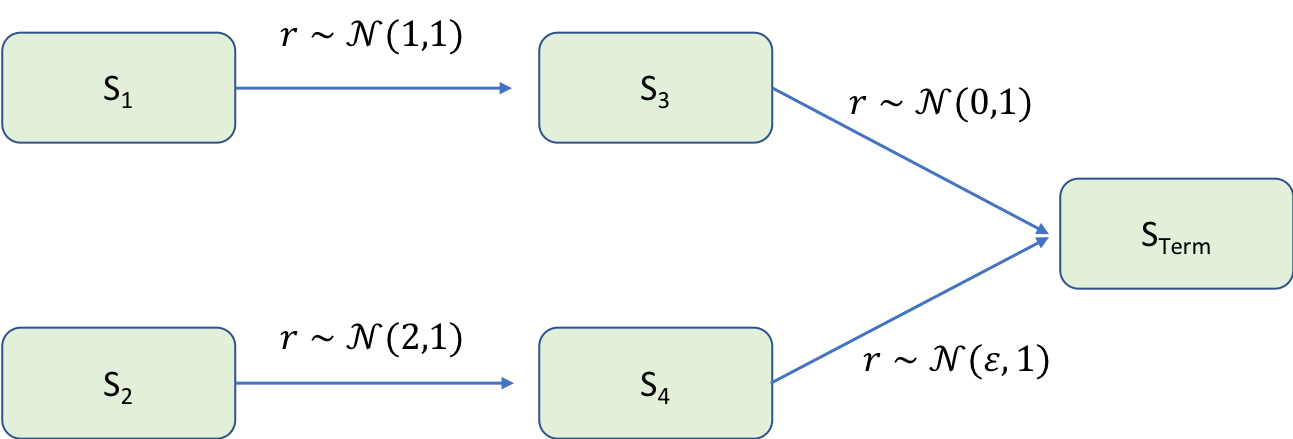
\includegraphics[width=\textwidth]{figures/td_vs_mc_FA.png}
    \caption{Example: MC vs. TD with function approximation.}
    \label{fig:td_vs_mc_FA}
\end{figure}

Consider the episodic MDP in Figure \ref{fig:td_vs_mc_FA}.
In this MDP there are two paths towards a terminal state. The first state in each path gives a large reward that determines most of the total return. The second state on each path gives a small reward that does not affect the total return by much, and therefore, the values of each of these second states are similar. We shall show that this value similarity may be exploited to reduce the variance in the estimates of the initial state values $\Value^{\policy}(\state_1)$ and $\Value^{\policy}(\state_2)$.

Formally, $\state_{Term}$ is a terminal state, and rewards are normally distributed with unit variance, as shown. There are no actions, and therefore for any $\policy$, $\Value^{\policy}(\state_1) = 1$, $\Value^{\policy}(\state_2) = 2+\varepsilon$, $\Value^{\policy}(\state_3) = 0$, and $\Value^{\policy}(\state_4) = \varepsilon$. We will particularly be interested in estimating $\Value^{\policy}(\state_1)$ and $\Value^{\policy}(\state_2)$.

Consider the case of no function approximation. Assume that we have sampled $N$ trajectories, where half start from $\state_1$, and the other half from $\state_2$. In this case, the MC estimates for $\widehat{\Value}^{\policy}(\state_1)$ and $\widehat{\Value}^{\policy}(\state_2)$ will each be based on $N/2$ samples, and their variance will therefore be $2 / ({N}/{2}) = 4/{N}$.

Let us recall the bootstrapping approach. We have that $\Value^{\policy}(\state_1) = \mathbb{E}\left[ \reward(\state_1)\right] + \Value^{\policy}(\state_3)$, and similarly, $\Value^{\policy}(\state_2) = \mathbb{E}\left[ \reward(\state_2)\right] + \Value^{\policy}(\state_4)$. Therefore, we can use the samples to first estimate $\widehat{\Value}^{\policy}(\state_3)$ and $\widehat{\Value}^{\policy}(\state_4)$, and then plug in to estimate $\widehat{\Value}^{\policy}(\state_1)$ and $\widehat{\Value}^{\policy}(\state_2)$.

Now, for small $\varepsilon$, we understand that the values $\Value^{\policy}(\state_3)$ and $\Value^{\policy}(\state_4)$ should be similar. One way to take this into account is to use function approximation that approximates $\Value^{\policy}(\state_3)$ and $\Value^{\policy}(\state_4)$ as \textit{the same} value, $\widehat{\Value}_{3/4}$. In this approximation we effectively use the full $N$ samples to estimate $\widehat{\Value}_{3/4}$, resulting in variance $1/{N}$. We can now use bootstrapping to estimate $\widehat{\Value}^{\policy}(\state_1)$ and $\widehat{\Value}^{\policy}(\state_2)$, which will result in variance $1 / {N}+ 1 / ({N}/{2}) = 3/{N}$, smaller than the MC estimate!

However, note that for $\varepsilon \neq 0$, the bootstrapping solution will also be biased: taking $N\to \infty$ we see that $\widehat{\Value}_{3/4}$ will converge to $\varepsilon/2$, and therefore $\widehat{\Value}^{\policy}(\state_1)$ and $\widehat{\Value}^{\policy}(\state_2)$ will converge to $1+\varepsilon/2$ and $2+\varepsilon/2$, respectively.

Thus, we see that bootstrapping, when combined with function approximation, allowed us to reduce variance by exploiting the similarity between values of different states, but at the cost of a possible bias in the expected solution. As it turns out, this phenomenon is not limited to the example above, but can be shown to hold more generally~\cite{kearns2000bias}. 
% \AT{I don't know of a general result about bias/variance that is simple enough to state in the book. Any ideas?}

In the following, we shall develop a rigorous formulation of bootstrapping with function approximation, and use it to suggest several approximation algorithms. We will also bound the bias incurred by this approach.

\subsection{Approximate Policy Evaluation: the Projected Bellman Equation}

% A key step in approximate policy iteration here is the policy evaluation: given $\policy$ we would like to approximate $\Value^\policy$. There are two main methods for approximate policy evaluation:
% \begin{enumerate}
% \item Direct approach: Evaluate $\Value^\policy(s)$ only for several states (e.g. by simulation) and interpolate, e.g., using least squares regression: $\FtrMtx \weights = \Pi \Value^\policy$. This method is simple, however, it has several drawbacks. The first is that value estimates typically have a large variance, as they accumulate rewards from multiple states in the future. The second is that we need to wait for full simulations to complete before updating the value estimate. Practically, this can take too long in some problems. 
% \item 
Recall from Chapter \ref{chapter:learning-model-free} that without function approximation, TD methods effectively compute a solution to the Bellman equation. With function approximation, this is no longer the case, as clearly  whatever solution TD methods converge to (if they converge at all), must depend on the function approximation. We shall start our investigation from a fundamental equation that takes function approximation into account -- the projected Bellman equation (PBE). We will use the PBE to define a particular approximation of the value function, and study its properties. We will later develop TD algorithms that estimate this approximation using sampling.

For technical simplicity, our analysis mainly considers linear function approximation. The algorithms we develop, however, can easily be extended to non-linear  approximation, and we will expand on particular cases where relevant. Let $\FtrMtx \in \mathbb{R}^{|\States|\times \nftrs}$ denote a matrix in which each row $\state$ is $\ftrs(\state)$, where without loss of generality we assume that the states are ordered as $1,2,\dots, |\States|$. 
Let $\ftrspace = \left\{ \FtrMtx \weights: \weights \in \mathbb{R}^{\nftrs} \right\}$ denote the linear subspace spanned by $\FtrMtx$.
Recall that $\Value^\policy(s)\in\mathbb{R}^{|\States|}$ satisfies the Bellman equation: $\Value^\policy = \operator^\policy \Value^\policy$. However, $\Value^\policy$ does not necessarily belong to $\ftrspace$, as we may not be able to accurately represent the true value function as a linear combination of our features. 

To write a `Bellman-like' equation that involves our function approximation, we proceed by projecting the Bellman operator $\operator^\policy$ onto $\ftrspace$, resulting in the PBE:
\begin{equation}\label{eq:PBE}
    \FtrMtx \weights = \Project_{\xi} \operator^\policy \{\FtrMtx \weights\},
\end{equation}
where $\Project_{\xi}$ is the projection operator onto $\ftrspace$ under some $\xi$-weighted Euclidean norm.

Let us try to intuitively interpret the PBE. We are looking for an approximate value function $\FtrMtx \weights \in \mathbb{R}^{|\States|}$, which by definition is within our linear approximation space, such that after we apply to it $\operator^\policy$, and project the result (which does not necessarily belong to $\ftrspace$ anymore) back to $\ftrspace$, we obtain the same approximate value. Since the true value is a fixed point of $\operator^\policy$, we have reason to believe that a fixed point of $\Project_{\xi}\operator^\policy$ may provide a reasonable approximation. In the following, we shall investigate this hypothesis, and build on Eq.~\eqref{eq:PBE} to develop various learning algorithms. We remark that the PBE is not the only way of defining an approximate value function, and other approaches have been proposed in the literature. However, the PBE is the basis for the most popular RL algorithms today.
    % \begin{equation*}
    %     \weights_k= \underset{\weights}{\operatorname{argmin}} \{||\FtrMtx \weights - T^{\policy_k}\FtrMtx \weights_k||_\xi^2\}.
    % \end{equation*}
% Includes:
% \begin{itemize}
% \item Temporal differences - TD(0): online solution of the PBE.
% % $\FtrMtx \weights = \Pi \operator^\policy \{\FtrMtx \weights\}$, where $\Pi$ is the projection operator onto $\mathcal{S}$ under some norm.\\
% \item Least-squares policy evaluation - LSPE(0): simulation-based form
% \begin{align*}\FtrMtx \weights_{k+1} = \Pi \operator^\policy \{\FtrMtx \weights_k\} + \mathrm{noise}.\end{align*} 
% \item Least-squares temporal differences - LSTD(0): batch solution of the PBE.
% \end{itemize}
% \end{enumerate}

% We now discuss the indirect approach to policy evaluation.

% Define the weighted Euclidean inner product:
% $$\langle V_1,V_2\rangle_\xi = {\sum_{i=1}^n \xi_i V_1(i)V_2(i)}, \ \ \xi_i\ge0,$$
% and the induced weighted Euclidean norm:
% $$||V||_\xi = \sqrt{\langle V,V\rangle_\xi} = \sqrt{\sum_{i=1}^n \xi_i V(i)^2}, \ \ \xi_i\ge0,$$
% and let $\Project_\xi$ be the operator of projection onto $\mathcal{S}$ w.r.t. this norm:
% \begin{align*}\Project_\xi V &=\underset{V' \in \mathcal{S}}{\operatorname{argmin}} \ ||V'-V||_\xi =\\
% &= \FtrMtx \weights \ \ \ \mathrm{s.t.} \ \ \weights = \underset{\weights' \in \mathbb{R}^k}{\operatorname{argmin}} \ ||\FtrMtx \weights' - V||_\xi.\end{align*}

% We want to solve the projected Bellman equation (PBE):
% \begin{equation}\label{eq:PBE}
% \FtrMtx \weights^*  = \Project_\xi \operator^\policy \FtrMtx \weights^*.
% \end{equation}
% The main reason to consider the approximation in \eqref{eq:PBE} is that, as we shall see, it will allow us to derive efficient sampling based algorithms with provable error guarantees.

\subsubsection{Existence, Uniqueness and Error Bound on PBE Solution}
We are interested in the following questions:
\begin{enumerate}
\item Does the PBE \eqref{eq:PBE} have a solution?
\item When is $\Project_\xi \operator^\policy$ a contraction, and what is its fixed point?
\item If $\Project_\xi \operator^\policy$ has a fixed point $\FtrMtx\weights^*$, how far is it from the best approximation possible, namely, $\Project_\xi  \Value^\policy$?
\end{enumerate}
Answering the first two points will characterize the approximate solution we seek. The third point above relates to the bias of the bootstrapping approach, as described in the example in Section \ref{ssec:APE_bootstrapping}. 

Let us assume the following:
\begin{assumption}\label{ass:recurrent}The Markov chain corresponding to $\policy$ has a single recurrent class and no transient states. We further let
$$\xi_j = \lim_{N\rightarrow \infty} \frac{1}{N} \sum_{\ttime=1}^N P(\state_\ttime=j|\state_0=\state)>0,$$
which is the probability of being in state $j$ when the process reaches its steady state, given any arbitrary $\state_0=\state$.
\end{assumption}
We have the following result:
\begin{proposition}\label{prop:PBE_contraction} Under Assumption \ref{ass:recurrent} we have that
\begin{enumerate}
\item $\Project_\xi \operator^\policy$ is a contraction operator with modulus $\gamma$ w.r.t. $||\cdot||_\xi$.
\item The unique fixed point $\FtrMtx \weights^*$ of $\Project_\xi \operator^\policy$ satisfies,
\begin{equation}\label{eq:bias_bound_1}
    ||\Value^\policy - \FtrMtx \weights^*||_\xi \le \frac{1}{1-\gamma}||\Value^\policy-\Project_\xi\Value^\policy||_\xi,
\end{equation}
and
\begin{equation}\label{eq:bias_bound_2}
||\Value^\policy - \FtrMtx \weights^*||_\xi^2 \le \frac{1}{1-\gamma^2}||\Value^\policy-\Project_\xi \Value^\policy||_\xi^2.
\end{equation}
\end{enumerate}
\end{proposition}

We remark that the bound in \eqref{eq:bias_bound_2} is stronger than the bound in  \eqref{eq:bias_bound_1} (show this!). We nevertheless include the bound \eqref{eq:bias_bound_1} for didactic purpose, as its proof is slightly different.
Proposition \ref{prop:PBE_contraction} shows that for the particular projection defined by weighting the Euclidean norm according to the stationary distribution of the Markov chain, we can both guarantee a solution to the PBE, and bound its bias with respect to $\Project_\xi \Value^\policy$ -- the best approximation of $\Value^\policy$ under the $\xi$ weighting. Fortunately, we shall see that this weighting is suitable for developing on-policy learning algorithms. However, the reader should note that for a different $\xi$, the conclusions of Proposition \ref{prop:PBE_contraction} do not necessarily hold.

\begin{proof}
We begin by showing the contraction property. We use two lemmas.
\begin{lemma}\label{lem:P_non_expansion} If $P^\policy$ is the transition matrix induced by $\policy$, then
$$\forall z \ \ ||P^\policy z||_\xi \le ||z||_\xi.$$
\end{lemma}
\begin{proof}
Let $p_{ij}$ be the components of $P^\policy$. For all $z \in \mathbb{R}^{|\States|}$:
$$||P^\policy z||_\xi^2 = \sum_i \xi_i\left(\sum_j p_{ij}z_j\right)^2 \underbrace{\leq}_{\textrm{Jensen}} \sum_i \xi_i \sum_j p_{ij} z_j^2 =  \sum_j z_j^2 \sum_i\xi_i p_{ij} = ||z||_\xi^2,$$
where the last equality uses a property of the stationary distribution $\xi_i$, $\sum_i\xi_i p_{ij}  =\xi_j$, and
$\sum_{j=1}^n\xi_j z_j^2 = ||z||_\xi^2.$
\end{proof}
\begin{lemma}\label{lem:pythagorian}
The projection $\Project_\xi$ obeys the Pythagorean theorem:
$$\forall J\in \mathbb{R}^{|\States|}, \widehat{J}\in \ftrspace: \ \ ||J-\widehat{J}||_\xi^2 = ||J-\Project_\xi J||_\xi^2 + ||\Project_\xi J - \widehat{J}||_\xi^2.$$
\end{lemma}
\begin{proof}
Observe that
$$||J-\widehat{J}||_\xi^2 = ||J-\Project_\xi J + \Project_\xi J - \widehat{J}||_\xi^2 = ||J-\Project_\xi J||_\xi^2 + ||\Project_\xi J - \widehat{J}||_\xi^2 + 2 \cdot \langle J-\Project_\xi J, \Project_\xi J - \widehat{J}\rangle_\xi.$$
We claim that $J-\Project_\xi J$ and $\Project_\xi J-\widehat{J}$ are orthogonal under $\langle\cdot,\cdot\rangle_\xi$ (this is known as the error orthogonality for weighted Euclidean-norm projections). To see this, recall that 
$$
\Project_\xi = \FtrMtx (\FtrMtx^T \Xi \FtrMtx)^{-1} \FtrMtx^T \Xi,
$$
so
$$
\Xi \Project_\xi = \Xi \FtrMtx (\FtrMtx^T \Xi \FtrMtx)^{-1} \FtrMtx^T \Xi = \Project_\xi^T \Xi.
$$
Now, 
\begin{equation*}
    \begin{split}
        \langle J-\Project_\xi J, \Project_\xi J - \widehat{J}\rangle_\xi &= (J-\Project_\xi J)^T \Xi (\Project_\xi J - \widehat{J}) \\
        &= J^T \Xi \Project_\xi J - J^T \Xi \widehat{J} - J^T \Project_\xi^T \Xi \Project_\xi J + J^T \Project_\xi^T \Xi \widehat{J} \\
        &= J^T \Xi \Project_\xi J - J^T \Xi \widehat{J} - J^T \Xi \Project_\xi \Project_\xi J + J^T \Xi\Project_\xi \widehat{J} \\
        &= J^T \Xi \Project_\xi J - J^T \Xi \Project_\xi J - J^T \Xi \widehat{J} + J^T \Xi \widehat{J} = 0,
    \end{split}
\end{equation*}
where in the penultimate equality we used that fact that $\Project_\xi \widehat{J} = \widehat{J}$, as $\widehat{J}\in \ftrspace$, and that $\Project_\xi \Project_\xi = \Project_\xi$, as projecting a vector that is already in $\ftrspace$ effects no change to the vector.
\end{proof}

We now claim that that $\Project_\xi$ is non-expansive.
\begin{lemma}
We have that $\forall {J}_1,{J}_2\in \mathbb{R}^{|\States|}, ||\Project_\xi {J}_1 - \Project_\xi {J}_2||_\xi \le ||{J}_1-{J}_2||_\xi$.
\end{lemma}

\begin{proof}
We have
$$||\Project_\xi {J}_1 - \Project_\xi {J}_2||_\xi^2 = ||\Project_\xi({J}_1-{J}_2)||_\xi^2 \le ||\Project_\xi({J}_1-{J}_2)||_\xi^2 + ||(I-\Project_\xi)({J}_1-{J}_2)||_\xi^2 = ||{J}_1-{J}_2||_\xi^2,$$
where the first inequality is by linearity of $\Project_\xi$, and the last equality is by the Pythagorean theorem of Lemma \ref{lem:pythagorian}, where we set $J={J}_1-{J}_2$ and $\widehat{J} = 0$.
\end{proof}

In order to prove the contraction of $\Project_\xi \operator^\policy$, $\forall {J}_1,{J}_2\in \mathbb{R}^{|\States|}$:
\begin{equation*}
\begin{split}
||\Project_\xi \operator^\policy {J}_1 - \Project_\xi \operator^\policy {J}_2||_\xi &\overset{\Project_\xi \textrm{ non-expansive}}{\le} ||\operator^\policy {J}_1 - \operator^\policy {J}_2||_\xi\\
&\overset{\textrm{definition of } \operator^\policy}{=} \gamma||P^\policy({J}_1-{J}_2)||_\xi \overset{\textrm{Lemma \ref{lem:P_non_expansion}}}{\le} \gamma||{J}_1-{J}_2||_\xi ,
\end{split}
\end{equation*}
and therefore $\Project_\xi \operator^\policy$ is a contraction operator.

We now prove the error bound in \eqref{eq:bias_bound_1}.
\begin{equation*}
\begin{split}
  ||\Value^\policy - \FtrMtx \weights^*||_\xi  &\leq ||\Value^\policy
-\Project_\xi \Value^\policy||_\xi + ||\Project_\xi \Value^\policy -\FtrMtx \weights^*||_\xi  \\
    &= ||\Value^\policy -\Project_\xi \Value^\policy||_\xi + ||\Project_\xi \operator^\policy \Value^\policy -\Project_\xi \operator^\policy\FtrMtx \weights^*||_\xi \\
&\leq ||\Value^\policy -\Project_\xi \Value^\policy||_\xi + \gamma||\Value^\policy-\FtrMtx \weights^*||_\xi,
\end{split}
\end{equation*}
where the first inequality is by the triangle inequality, the second equality is since $\Value^\policy$ is $\operator^\policy$'s fixed point, and $\FtrMtx \weights^*$ is $\Project_\xi \operator^\policy$'s fixed point, and the second inequality is by the contraction of $\Project_\xi \operator^\policy$. Rearranging gives \eqref{eq:bias_bound_1}.

We proceed to prove the error bound \eqref{eq:bias_bound_2}.
\begin{equation}
\begin{split}
  ||\Value^\policy - \FtrMtx \weights^*||_\xi^2  &= ||\Value^\policy
-\Project_\xi \Value^\policy||_\xi^2 + ||\Project_\xi \Value^\policy -\FtrMtx \weights^*||_\xi^2  \\
    &= ||\Value^\policy -\Project_\xi \Value^\policy||_\xi^2 + ||\Project_\xi \operator^\policy \Value^\policy -\Project_\xi \operator^\policy\FtrMtx \weights^*||_\xi^2 \\
&\leq ||\Value^\policy -\Project_\xi \Value^\policy||_\xi^2 + \gamma^2||\Value^\policy-\FtrMtx \weights^*||_\xi^2,
\end{split}
\end{equation}
where the first equality is by the Pythagorean theorem, and the remainder follows similarly to the proof of \eqref{eq:bias_bound_1} above.
% the second equality is since $\Value^\policy$ is $\operator^\policy$'s fixed point, and $\FtrMtx \weights^*$ is $\Project_\xi \operator^\policy$'s fixed point, and the inequality is by the contraction of $\Project_\xi \operator^\policy$.

% Therefore
% $$||\Value^\policy - \FtrMtx \weights^*||_\xi^2 \le \frac{1}{1-\gamma^2}||\Value^\policy-\Project_\xi \Value^\policy||_\xi^2.$$
\end{proof}

% \begin{remark}
% A weaker error bound of $||\Value^\policy - \FtrMtx \weights^*||_\xi \le \frac{1}{1-\gamma}||\Value^\policy-\Project_\xi
% \Value^\policy||_\xi$ may be obtained by the following argument:
% \begin{equation}
% \begin{split}
%   ||\Value^\policy - \FtrMtx \weights^*||_\xi  &\leq ||\Value^\policy
% -\Project_\xi \Value^\policy||_\xi + ||\Project_\xi \Value^\policy -\FtrMtx \weights^*||_\xi  \\
%     &= ||\Value^\policy -\Project_\xi \Value^\policy||_\xi + ||\Project_\xi \operator^\policy \Value^\policy -\Project_\xi \operator^\policy\FtrMtx \weights^*||_\xi \\
% &\leq ||\Value^\policy -\Project_\xi \Value^\policy||_\xi + \gamma||\Value^\policy-\FtrMtx \weights^*||_\xi,
% \end{split}
% \end{equation}
% where the first inequality is by the triangle inequality.
% \end{remark}
% \begin{remark}
% The error bounds in this section are in the $\| \cdot \|_\xi$ norm, while the approximate policy iteration error bounds of Theorem \ref{thm:API} are in the $\| \cdot \|_\infty$ norm. In general, for large or continuous state spaces, an $\| \cdot \|_\xi$ norm error bound does not provide a strong guarantee on the error in the $\| \cdot \|_\infty$ norm, and the results of Theorem \ref{thm:API} therefore do not apply. A result similar to that of Theorem \ref{thm:API} may be shown to hold in the $\| \cdot \|_\xi$ norm, however this is much more complicated, and beyond the scope of this course.
% \end{remark}
% \begin{remark}
% At this point, the reader should wonder why the PBE solution is sought instead of $\Project_\xi \Value^\policy$. In fact, an algorithm for estimating $\Project_\xi \Value^\policy$ can easily be derived using regression. For example, consider an algorithm that samples states $s_1,\dots,s_N \sim \xi$, and from each state $s_i$ runs a trajectory in the MDP following policy $\policy$. Let $y_i$ denote the discounted return in that trajectory. Then, a least squares fit:
% \begin{equation*}
%     \min_\weights \frac{1}{2}\sum_{i=1}^{N} \left(y_i - \ftrs(s_i)^\top\weights\right)^2
% \end{equation*}
% would converge to $\Project_\xi \Value^\policy$ as $N\to \infty$. However, such an algorithm would suffer a high variance, since the discounted return in the whole trajectory often has a high variance. The PBE approach typically has lower variance, since it only considers 1-step transitions instead of complete trajectories. However, it may have a \emph{bias}, as seen by the error bound in Proposition \ref{prop:PBE_contraction}. We thus have a bias-variance tradeoff between the direct and indirect approaches to policy evaluation.
% \end{remark}

\subsection{Solution Techniques for the Projected Bellman Equation}\label{ssec:TD_solution_techniques}
We now move to solving the projected Bellman equation. 
In Section \ref{ssec:least_squares_regression} we presented a closed-form solution for linear least squares and an algorithm based on SGD. We use these approaches as inspiration for a sampling-based solution for the PBE.

Using the explicit formulation of the projection $\Project_\xi$, we see that the PBE solution is some $\widehat{\Value} = \FtrMtx \weights^*$ where $\weights^*$ solves
$$\weights^* = \underset{{\weights \in \mathbb{R}^\nftrs}}{\operatorname{argmin}} \ ||\FtrMtx \weights - (R^\policy+\gamma P^\policy\FtrMtx \weights^*)||_\xi^2.$$
Setting the gradient to $0$, we get
$$\FtrMtx^T \Xi (\FtrMtx \weights^* - (R^\policy+\gamma P^\policy \FtrMtx \weights^*)) = 0.$$
% where $\Xi = \textrm{diag} \ (\xi_1,...,\xi_n)$.\\
% This is in fact the orthogonality condition from random signals.\\
Equivalently we can write
$$A \weights^* = b,$$
where
\begin{equation}\label{eq:A_b_TD}
A = \FtrMtx^T \Xi(I-\gamma P^\policy) \FtrMtx, \ \ b = \FtrMtx^T\Xi R^\policy.
\end{equation}

\paragraph{Solution approaches:}
\begin{enumerate}
\item \textbf{Matrix inversion (Least Squares Temporal Differences, LSTD)}: 
We have that $$\weights^* = A^{-1}b.$$
In order to evaluate $A,b$, we use simulation.
\begin{proposition}\label{prop:TD_expectations}
    We have that 
    \begin{equation*}
        \mathbb{E}_{\state\sim\xi}\left[ {\ftrs}(\state) r(\state,\policy(\state)) \right] = b,
    \end{equation*}
    and
    \begin{equation*}
        \mathbb{E}_{\state\sim\xi, \state'\sim P^\policy(\cdot|\state)}\left[ {\ftrs}(\state)( {\ftrs}^T(\state)-\gamma {\ftrs}^T(\state')) \right] = A.
    \end{equation*}
\end{proposition}
\begin{proof}
    We have
    \begin{equation*}
        \mathbb{E}_{\state\sim\xi}\left[ {\ftrs}(\state) r(\state,\policy(\state)) \right] = \sum_{\state}  {\ftrs}(\state) \xi(\state) r(\state,\policy(\state)) = \FtrMtx^T\Xi R^\policy = b.
    \end{equation*}
    Also,
    \begin{equation*}
    \begin{split}
        &\mathbb{E}_{\state\sim\xi, \state'\sim P^\policy(\cdot|\state)}\left[ {\ftrs}(\state)( {\ftrs}^T(\state)-\gamma {\ftrs}^T(\state')) \right] \\
        &= \sum_{\state,\state'} \xi(\state)P^\policy(\state'|\state){\ftrs}(\state)( {\ftrs}^T(\state)-\gamma {\ftrs}^T(\state')) \\
        &= \sum_{\state} {\ftrs}(\state) \xi(\state){\ftrs}^T(\state) - \gamma\sum_{\state}{\ftrs}(\state)\xi(\state)\sum_{\state'}P^\policy(\state'|\state){\ftrs}^T(\state')\\
        &= \FtrMtx^T \Xi \FtrMtx -\gamma \FtrMtx^T\Xi P^\policy \FtrMtx = A.
    \end{split}
    \end{equation*}
\end{proof}
We now propose the following estimates to $A$ and $b$. 
% Simulate a sequence of $N$ state-action pairs $\state_1,\action_1,\state_2,\action_2,\dots,\state_N,\action_N,\state_{N+1}$ using the policy $\policy$, i.e., $\action_i \sim \policy(\cdot|\state_i)$, and starting from an arbitrary $\state_0$. The Least Squares Temporal Difference algorithm (LSTD) estimates are given by
% \begin{align*}
% \widehat{b}_N &= \frac{1}{N} \sum_{t=1}^N  {\ftrs}(\state_\ttime) r(\state_\ttime,\policy(\state_\ttime)) \end{align*}
% and 
% \begin{align*}
% \widehat{A}_N &=
% \frac{1}{N} \sum_{t=1}^N {\ftrs}(\state_\ttime)( {\ftrs}^T(\state_\ttime)-\gamma {\ftrs}^T(\state_{\ttime+1})).
% \end{align*}

\begin{algorithm}[H]
\caption{Least Squares Temporal Difference (LSTD)}
\begin{algorithmic}[1]
\State \textbf{Input:} Policy $\policy$, discount factor $\gamma$, number of steps $N$
\State Initialize $\state_0$ arbitrarily
\State \textbf{For} {$\ttime = 1$ to $N$}
    \State \quad Simulate action $\action_\ttime \sim \policy(\cdot \mid \state_\ttime)$
    \State \quad Observe new state $\state_{\ttime+1}$
\State Compute $\widehat{b}_N$:
\[
\widehat{b}_N = \frac{1}{N} \sum_{\ttime=1}^N \ftrs(\state_\ttime) \reward(\state_\ttime, \policy(\state_\ttime))
\]
\State Compute $\widehat{A}_N$:
\[
\widehat{A}_N = \frac{1}{N} \sum_{\ttime=1}^N \ftrs(\state_\ttime)(\ftrs^T(\state_\ttime) - \gamma \ftrs^T(\state_{\ttime+1}))
\]
\State \textbf{Return} $\weights_N = \widehat{A}_N^{-1}\widehat{b}_N$
\end{algorithmic}
\end{algorithm}

From the ergodicity property of Markov chains (Theorem \ref{thm:finite_Markov_chains}), we have the following result.
\begin{proposition}
We have that 
\begin{equation*}
    \lim_{N\to \infty} \widehat{b}_N = b, \quad \lim_{N\to \infty} \widehat{A}_N = A
\end{equation*}
with probability 1.
\end{proposition}

\item \textbf{Projected Value Iteration:}
Consider the iterative solution,
$$\FtrMtx \weights_{n+1} = \Project_\xi \operator^\policy \FtrMtx \weights_n = \Project_\xi(R^\policy+\gamma P^\policy \FtrMtx \weights_n),$$
which converges to $\weights^*$ since $\Project_\xi \operator^\policy$ is a contraction operator.\\

Recalling that $\Project_\xi$ relates to a least squares regression problem, the solution above describes a sequence of least squares regression problems. For the $(n+1)$'th regression problem, our independent variable is the state, $\state$, and the dependent variable is $\reward(\state) +\gamma \sum_{\state'}P^\policy(\state'|\state) \ftrs(\state')^T \weights_n$.

If we sample trajectories from $\policy$, after some mixing time $\ttime$, a pair of consecutive state $\state_\ttime, \state_{\ttime+1}$ are sampled from $\xi(\state)$ and $P^\policy(\state'|\state)\xi(\state)$, respectively. Therefore, we can define the samples for the least squares regression problem as $\left\{(\state_\ttime, \reward(\state_\ttime) +\gamma \ftrs(\state_{\ttime+1})^T \weights_n), \dots  (\state_{\ttime+N}, \reward(\state_{\ttime+N}) +\gamma \ftrs(\state_{\ttime+N+1})^T \weights_n)\right\}$.

% The projection step is
% $$ \weights_{n+1} = \underset{\weights}{\operatorname{argmin}}||\FtrMtx \weights - (R^\policy+\gamma P^\policy \FtrMtx \weights_n)||_\xi^2.$$
% Setting the gradient to $0$ w.r.t. $\weights$:
% $$\FtrMtx^T \Xi(\FtrMtx \weights_{n+1} - (R^\policy+\gamma P^\policy \FtrMtx \weights_n)) = 0$$
% $$\Rightarrow \weights_{n+1} = \weights_n - (\FtrMtx^T\Xi\FtrMtx)^{-1}(A \weights_n-b).$$
% So we can approximate
% $$\weights_{n+1} = \weights_n - G_n(A_n \weights_n -b_n),$$
% where
% $$G_n^{-1} \approx \frac{1}{n+1} \sum_{t=0}^n  {\ftrs}(\state_\ttime) {\ftrs}(\state_\ttime)^T \Rightarrow G_n \approx (\FtrMtx^T \Xi \FtrMtx)^{-1}.$$
% We observe that $A_n,b_n,G_n$ can also be computed via the SA algorithm.

\begin{remark}\label{remark:non_linear_PVI}
Projected value iteration can be used with a more general regression algorithm. Let $\Project_{gen}$ denote a general regression algorithm, such as a non-linear least squares fit, a neural network, or even a non-parametric regression such as K-nearest neighbors. We can consider the iterative algorithm:
$$\widehat{\Value}(\weights_{n+1}) = \Project_{gen} \operator^\policy \widehat{\Value}(\weights_{n}).$$
To realize this algorithm, we use the same samples as above, and only replace the regression algorithm. Note that convergence in this case is not guaranteed, as in general, $\Project_{gen} \operator^\policy$ is not necessarily a contraction in any norm.
\end{remark}

\item \textbf{Stochastic Approximation -- TD(0):} Consider the function-approximation variant of the TD(0) algorithm (cf. Section \ref{sec:TD})
% \begin{equation}\label{eq:TD_func_approx}
%     \weights_{\ttime+1} = \weights_\ttime + \alpha_\ttime \underbrace{( \reward(\state_\ttime,\policy(\state_\ttime)) +\discount {\ftrs}(\state_{\ttime+1})^\top \weights_\ttime - {\ftrs}(\state_{\ttime})^\top \weights_\ttime)}_{\textrm{temporal difference}} \ftrs(\state_{\ttime}),
% \end{equation}

\begin{algorithm}[H]
\caption{TD(0) with Linear Function Approximation}
\begin{algorithmic}[1]
\State \textbf{Initialize:} Set $\weights_0 = 0$.
\State \textbf{For} {$\ttime = 0, 1, 2, \dots$}
    \State \quad Observe: $(\state_\ttime, \action_\ttime, \reward_\ttime, \state_{\ttime+1})$.
    \State \quad Update:
    \begin{equation}\label{eq:TD_func_approx}
    \weights_{\ttime+1} = \weights_\ttime + \alpha_\ttime \underbrace{( \reward(\state_\ttime,\policy(\state_\ttime)) +\discount {\ftrs}(\state_{\ttime+1})^\top \weights_\ttime - {\ftrs}(\state_{\ttime})^\top \weights_\ttime)}_{\textrm{temporal difference}} \ftrs(\state_{\ttime}).
\end{equation}
\end{algorithmic}
\end{algorithm}

where the temporal difference term is the approximation (w.r.t. the weights at time $\ttime$) of $\reward(\state_\ttime,\policy(s_\ttime)) +\discount \Value(\state_{\ttime+1}) - \Value(s_\ttime)$.
\\
This algorithm can be written as a stochastic approximation:
\begin{equation*}
    \weights_{\ttime+1} = \weights_\ttime + \alpha_\ttime ( b -  A \weights_\ttime + \omega_\ttime ),
\end{equation*}
where $A$ and $b$ are defined in \eqref{eq:A_b_TD}, and $\omega_\ttime$ is a noise term. The corresponding ODE is $\dot{\weights} = b -  A \weights_\ttime$, with a unique stable fixed point at $\weights^* = A^{-1}b$. 

\begin{remark}
    In the tabular setting, we proved the convergence of TD(0) using the contraction method for stochastic approximation. Here, we cannot use this approach, as the contraction in TD(0), which follows from the Bellman equation, applies to the values of each state. However, with function approximation, we iterate over the weights $\weights_\ttime$ and not over the values for each state, and for these weights the contraction does not necessarily hold. For this reason, we shall seek a convergence proof based on the ODE method.
\end{remark}

We next prove convergence of TD(0). For simplicity, we will consider a somewhat synthetic version of TD(0) where at each iteration $\ttime$, the state $\state_\ttime$ is drawn i.i.d. from the stationary distribution $\xi(\state)$, and the next state $\state_{\ttime+1}$ in the update rule is drawn from $P^\policy(\state'|\state = \state_\ttime)$, respectively. This will allow us to claim that the noise term satisfies $\E[\omega_\ttime|h_{\ttime-1}]=0$. 


\begin{theorem}
    Consider the following iterative algorithm:
    \begin{equation*}\label{eq:TD_func_approx_iid}
    \weights_{\ttime+1} = \weights_\ttime + \alpha_\ttime ( \reward(\state_\ttime,\policy(\state_\ttime)) +\discount {\ftrs}(\state_{\ttime}')^\top \weights_\ttime - {\ftrs}(\state_{\ttime})^\top \weights_\ttime) \ftrs(\state_{\ttime}),
\end{equation*}
where $\state_\ttime\sim \xi(\state)$ i.i.d., and $\state_{\ttime}' \sim P^\policy(\state'|\state = \state_\ttime)$ independently of the history up to time $t$. Assume that $\FtrMtx$ is full rank. Let the step sizes satisfy $\sum_\ttime
\alpha_\ttime
=\infty $, and 
$\sum_\ttime \alpha_\ttime^2=O(1)$. Then $\weights_\ttime$
converges with probability $1$ to $\weights^*= A^{-1}b$.
\end{theorem}
\begin{proof}
    We write Eq.~\eqref{eq:TD_func_approx_iid} as 
    \begin{equation*}
    \weights_{\ttime+1} = \weights_\ttime + \alpha_\ttime ( b -  A \weights_\ttime + \omega_\ttime ),
\end{equation*}
where the noise $\omega_\ttime = \reward(\state_\ttime,\policy(\state_\ttime))\ftrs(\state_{\ttime}) - b +  (\discount{\ftrs}(\state_{\ttime}')^\top - {\ftrs}(\state_{\ttime})^\top) \weights_\ttime \ftrs(\state_{\ttime}) + A \weights_\ttime$ satisfies: 
\begin{equation*}
\E[\omega_\ttime|h_{\ttime-1}]= \E[\omega_\ttime|\weights_\ttime]= 0,
\end{equation*}
where the first equality is since the states are drawn i.i.d., and the second is from Proposition \ref{prop:TD_expectations}.
We would like to use Theorem \ref{thm:stoch-approx-ODE-linear} to show convergence. From Proposition \ref{prop:PBE_contraction} we already know that $\weights^*$ corresponds to the unique fixed point of the linear dynamical system $\safunc(\weights) = -A\weights + b$.
We proceed to show that $\weights^*$ is
globally asymptotically stable, by showing that the eigenvalues of $A$ have a positive real part. Let $z \in \mathbb{R}^{|\States|}$. We have that
\begin{equation*}
\begin{split}
    z^T \Xi P^\policy z &= z^T \Xi^{1/2} \Xi^{1/2} P^\policy z \\
    &\leq \| \Xi^{1/2} z \| \| \Xi^{1/2} P^\policy z \| \\
    &=\| z \|_{\xi} \| P^\policy z \|_{\xi} \\
    &\leq \| z \|_{\xi}\| z \|_{\xi} = z^T \Xi z.
\end{split}
\end{equation*}
where the first inequality is by Cauchy-Schwarz, and the second is by Lemma \ref{lem:P_non_expansion}.

We claim that the matrix $\Xi(I-\gamma P^\policy)$ is positive definite. To see this, observe that for any $z \in \mathbb{R}^{|\States|}\neq 0$ we have
\begin{equation}\label{eq:TD_convergnece_proof_eq1}
    z^T\Xi(I-\gamma P^\policy)z = z^T \Xi z - \gamma z^T \Xi P^\policy z \geq z^T \Xi z - \gamma z^T \Xi z = (1-\gamma) \|z\|_{\xi} > 0.
\end{equation}
We now claim that $A= \FtrMtx^T \Xi(I-\gamma P^\policy) \FtrMtx$ is positive definite. Assume by negation that for some $\theta \in \mathbb{R}^\nftrs$, $\theta\neq 0$ we have $\theta^T\FtrMtx^T\Xi(I-\gamma P^\policy)\FtrMtx\theta \leq 0$. If $\FtrMtx$ is full rank, then $z = \FtrMtx\theta \in \mathbb{R}^{|\States|} \neq 0$, contradicting Eq.~\eqref{eq:TD_convergnece_proof_eq1}. The claim that the eigen-values of $A$ have a positive real part is not immediate from the positive definiteness established above since $A$ is not necessarily symmetric. To show this, let $\lambda \in \mathbb{C} = \alpha + \beta i$ be an eigenvalue of $A$, and let $v \in \mathbb{C}^\nftrs = x + iy$, where $x,y\in \mathbb{R}^\nftrs$, be its associated right eigenvector. We have that $(A-\lambda)v = 0$, therefore
$$
((A - \alpha) -\beta i)(x + iy) = 0,
$$
therefore $(A-\alpha)x + \beta y = 0$ and $(A-\alpha)y - \beta x = 0$. Multiplying these two equations by $x^T$ and $y^T$, respectively, and summing we obtain
$$
x^T(A-\alpha)x + y^T(A-\alpha)y = - x^T\beta y + y^T\beta x = \beta(y^Tx - x^Ty) = 0.
$$
Therefore,
$$
\alpha = \frac{x^TAx + y^TAy}{x^Tx + y^Ty} > 0.
$$
\end{proof}

\begin{remark}
A similar convergence result holds for the standard TD(0) of Eq.~\ref{eq:TD_func_approx}, using a more sophisticated proof technique that accounts for noise that is correlated (depends on the state). The main idea is to show that since the Markov chain mixes quickly, the \textit{average} noise is still close to zero with high probability~\cite{TsitsiklisVR97}.
\end{remark}


\end{enumerate}
% \begin{remark}
For a general (not necessarily linear) function approximation, the TD(0) algorithm takes the form:
\begin{equation*}
    \weights_{n+1} = \weights_n + \alpha_n \left( \reward(\state_n,\policy(\state_n)) + \discount\widehat{\Value}(\state_{n+1},\weights_n) - \widehat{\Value}(\state_{n},\weights_n) \right) \nabla_{\weights} \widehat{\Value}(\state_n,\weights).
\end{equation*}
It can be derived as a stochastic gradient descent algorithm for the loss function
\begin{equation*}
    Loss(\weights) = ||\widehat{\Value}(\state,\weights) - \Value^\policy(\state)||_\xi,
\end{equation*}
and replacing the unknown $\Value^\policy(\state)$ with a TD-style estimator $\reward(\state,\policy(\state))+\discount \widehat{\Value}(\state',\weights)$.
% \end{remark}
%\end{document}
%~

\subsection{Episodic MDPs}

We can extend the learning algorithms above to the  episodic MDP setting, by removing the discount factor, and explicitly setting the value of a goal state to $0$, similarly to Section \ref{ssec:mfrl_episodic}. For example, the TD(0) algorithm would be modified to,
\begin{equation*}\label{eq:TD_func_approx_ssp}
    \weights_{\ttime+1} = \begin{cases}
        \weights_\ttime + \alpha_\ttime ( \reward(\state_\ttime,\policy(\state_\ttime)) +{\ftrs}(\state_{\ttime+1})^\top \weights_\ttime - {\ftrs}(\state_{\ttime})^\top \weights_\ttime) \ftrs(\state_{\ttime}), & \state_{\ttime+1} \notin \States_G \\
        \weights_\ttime + \alpha_\ttime ( \reward(\state_\ttime,\policy(\state_\ttime)) - {\ftrs}(\state_{\ttime})^\top \weights_\ttime) \ftrs(\state_{\ttime}), & \state_{\ttime+1} \in \States_G
    \end{cases}.
\end{equation*}
Setting the value of goal states to $0$ is critical with function approximation (and is a common `bug' in episodic MDP implementations), as with function approximation, updates to the non-goal states will impact the approximation of goal state values, and  nothing in the algorithm will push to correct these errors.

\section{Approximate Policy Iteration}

So far we have developed various algorithms for approximating the value of a fixed policy $\policy$. Our main interest, however, is finding a \textit{good} policy. Similarly to RL without function approximation, we will consider two different approaches, based on either policy iteration or value iteration. In this section we consider approximate policy iteration.

% \subsection{Approximate Policy Iteration}

\paragraph{The general algorithm:} iterate between projection of $\Value^{\policy_k}$ onto $\ftrspace$ and policy improvement via a greedy policy update w.r.t. the projected $\Value^{\policy_k}$.
%$\operator^\policy$ (recall $\operator^\policy V = R^\policy + \gamma  P\policy V$, and Bellman's operator satisfies $TV = \max_{\policy \in \Pi} \operator^\policy V$):

\vspace{20pt}
\tikzstyle{block} = [rectangle, draw,
    text width=7em, text centered, rounded corners, minimum height=4em]
\tikzstyle{line} = [draw, -latex']
\begin{tikzpicture}[node distance = 2cm, auto]
    % Place nodes
    \node [block, node distance=1.5in, text width=3em] (a) {Guess $\policy_0$};
    \node [block, node distance=2in, right of =a, text width=10em] (b) {Evaluate: \\ $\widehat{\Value}_k=\FtrMtx \weights_k \approx \Value^{\policy_{k}}$ };
    \node [block, node distance=2in, right of = b, text width=10em] (c) {Improve: $\policy_{k+1}\approx \textrm{greedy}(\widehat{\Value}_k)$};
    % Draw edges
    \path [line] (a) -- (b);
    \path [line] (b) -- (c);
    \path [line,rounded corners] (c) |- ($(b.south east) + (0.5,-0.5)$) -| (b);
\end{tikzpicture}
\vspace{20pt}

A key question in approximate policy iteration, is how errors in the value-function approximation, and possibly also errors in the greedy policy update, affect the error in the final policy. The next result shows that if we can guarantee that the approximation errors are bounded at each step of the algorithm, then the error in the final policy will also be bounded. This result suggests that approximate policy iteration is a fundamentally sound idea.

\begin{theorem}\label{thm:API}
If for each iteration $k$ the policies are approximated well over $\States$:
\begin{equation}\label{eq:approx_pi_1}
\|\widehat{\Value}_k(\state)-\Value^{\policy_k}(\state)\|_\infty \le \delta,
\end{equation}
and policy improvement approximates well
\begin{equation}\label{eq:approx_pi_2}
\|\operator^{\policy_{k+1}}\widehat{\Value}_k - \operator\widehat{\Value}_k\|_\infty < \varepsilon,
\end{equation}
Then
$$ \limsup_k \ \| \Value^{\policy_k}(\state)-\Value^*(\state)\|_\infty \le \frac{\varepsilon+2\gamma\delta}{(1-\gamma)^2}.$$
\end{theorem}
\sloppy To understand the policy improvement approximation term \eqref{eq:approx_pi_2}, recall that the Bellman operator $\operator\widehat{\Value}_k$ corresponds to a greedy policy improvement step, $\policy_{\textrm{greedy}}\left(\widehat{\Value}_k\right)(\state) = \argmax_{\action} \reward(\state,\action) + \discount \sum_{\state'} \transitionprob(\state'|\state,\action)\widehat{\Value}_k(\state')$. Suppose we cannot perform the $\argmax$ accurately for every state when computing the next policy $\policy_{k+1}$, that is, $\policy_{k+1} \neq \policy_{\textrm{greedy}}\left(\widehat{\Value}_k\right)$. The condition \eqref{eq:approx_pi_2} ensures that $\policy_{k+1}$ is not too far off, in that $\reward(\state,\policy_{k+1}(\state)) + \discount \sum_{\state'} \transitionprob(\state'|\state,\policy_{k+1}(\state))\widehat{\Value}_k(\state')$ is not more than $\varepsilon$ away from $\policy_{\textrm{greedy}}\left(\widehat{\Value}_k\right)(\state)$.
\begin{proof}
    Let $e$ denote a vector of ones. From the contraction property of $\operator$ and $\operator^{\policy_{k+1}}$ we have that
    \begin{equation*}
        \| \operator^{\policy_{k+1}} \widehat{\Value}_k - \operator^{\policy_{k+1}}\Value^{\policy_k} \|_\infty \leq \discount \delta,
    \end{equation*}
    \begin{equation*}
        \| \operator \widehat{\Value}_k - \operator\Value^{\policy_k} \|_\infty \leq \discount \delta.
    \end{equation*}
    Therefore, 

    \begin{equation}\label{eq:approx_pi_3}
        \operator^{\policy_{k+1}}\Value^{\policy_k} \geq \operator^{\policy_{k+1}}\widehat{\Value}_k - \discount \delta e \geq \operator\widehat{\Value}_k - (\varepsilon + \discount \delta) e \geq \operator\Value^{\policy_k} - (\varepsilon + 2 \discount \delta) e
    \end{equation}
    where the inequalities are element-wise, the first inequality is by \eqref{eq:approx_pi_3}, the second inequality is by \eqref{eq:approx_pi_2}, and the last inequality is again by \eqref{eq:approx_pi_3}.
    Now, by definition of $\operator$,
    \begin{equation*}
        \operator\Value^{\policy_k} - (\varepsilon + 2 \discount \delta) e \geq \operator^{\policy_k}\Value^{\policy_k} - (\varepsilon + 2 \discount \delta) e = \Value^{\policy_k} - (\varepsilon + 2 \discount \delta) e,
    \end{equation*}
    so we have
    \begin{equation}\label{eq:approx_pi_4}
        \operator^{\policy_{k+1}}\Value^{\policy_k} \geq \Value^{\policy_k} - (\varepsilon + 2 \discount \delta) e.
    \end{equation}
    Since $\operator^{\policy_{k+1}}$ is a contraction and linear, we have that for any $\Value$ and a scalar $\alpha > 0$,
    \begin{equation*}
        \| \operator^{\policy_{k+1}}(\Value - \alpha e) - \operator^{\policy_{k+1}}\Value \|_\infty \leq \discount \alpha \| e \|_\infty = \discount \alpha.
    \end{equation*}
    Therefore, 
    \begin{equation}\label{eq:approx_pi_5}
        \operator^{\policy_{k+1}}(\Value - \alpha e) \geq \operator^{\policy_{k+1}}\Value - \discount \alpha e,
    \end{equation}
    and
    \begin{equation}\label{eq:approx_pi_5b}
        \operator^{\policy_{k+1}}(\Value - \alpha e) \leq \operator^{\policy_{k+1}}\Value + \discount \alpha e.
    \end{equation}
    Recalling that $\operator^{\policy_{k+1}}$ is a monotone operator (see proof of Lemma \ref{lemma:policy_improvement}), applying $\operator^{\policy_{k+1}}$ to both sides of \eqref{eq:approx_pi_4} and using \eqref{eq:approx_pi_5} we obtain:
    \begin{equation*}
    \left(\operator^{\policy_{k+1}}\right)^2\Value^{\policy_k} \geq \operator^{\policy_{k+1}}\Value^{\policy_k} - \discount(\varepsilon + 2 \discount \delta) e.
    \end{equation*}
    Similarly, applying $\left(\operator^{\policy_{k+1}}\right)^m$ to both sides of \eqref{eq:approx_pi_4} gives
    \begin{equation}\label{eq:approx_pi_6}
    \left(\operator^{\policy_{k+1}}\right)^{m+1}\Value^{\policy_k} \geq \left(\operator^{\policy_{k+1}}\right)^m\Value^{\policy_k} - \discount^m(\varepsilon + 2 \discount \delta) e.
    \end{equation}
    Now, consider the telescoping sum 
    \begin{equation*}    \left(\operator^{\policy_{k+1}}\right)^{n}\Value^{\policy_k} - \Value^{\policy_k} = \sum_{m=0}^{n-1}\left(\operator^{\policy_{k+1}}\right)^{m+1}\Value^{\policy_k} - \left(\operator^{\policy_{k+1}}\right)^m\Value^{\policy_k} \geq \left(\sum_{m=0}^{n-1}\discount^m\right)(\varepsilon + 2 \discount \delta) e,
    \end{equation*}
    where in the last equality we plugged \eqref{eq:approx_pi_6}. Taking $n \to \infty$ we obtain:
    \begin{equation}\label{eq:approx_pi_7}
        \Value^{\policy_{k+1}} - \Value^{\policy_k} \geq \frac{\varepsilon + 2 \discount \delta}{1 - \discount}e.
    \end{equation}
    Now,
    \begin{equation*}
    \begin{split}
        -\Value^{\policy_{k+1}} = -\operator^{\policy_{k+1}}\Value^{\policy_{k+1}} &= -\operator^{\policy_{k+1}}\Value^{\policy_{k}} - \left( \operator^{\policy_{k+1}}\Value^{\policy_{k+1}} - \operator^{\policy_{k+1}}\Value^{\policy_{k}}\right) \\ 
        &\leq -\operator^{\policy_{k+1}}\left(\Value^{\policy_{k}} + \frac{\varepsilon + 2 \discount \delta}{1 - \discount}e \right)\\
        &= \operator^{\policy_{k+1}}\left(-\Value^{\policy_{k}} - \frac{\varepsilon + 2 \discount \delta}{1 - \discount}e \right)\\
        &\leq -\operator^{\policy_{k+1}}\Value^{\policy_{k}} + \discount \frac{\varepsilon + 2 \discount \delta}{1 - \discount}e,
    \end{split}
    \end{equation*}
    where the first inequality is by \eqref{eq:approx_pi_7} and the second is by \eqref{eq:approx_pi_5b}.

    We next have,
    \begin{equation}\label{eq:approx_pi_8}
        \Value^{*} - \Value^{\policy_{k+1}} \leq \Value^{*} -\operator^{\policy_{k+1}}\Value^{\policy_{k}} + \discount \frac{\varepsilon + 2 \discount \delta}{1 - \discount}e.
    \end{equation}
    From the contraction of $\operator$ we have:
    \begin{equation}\label{eq:approx_pi_contraction}
        \Value^{*} - \operator \Value^{\policy_{k}} = \operator\Value^{*} - \operator \Value^{\policy_{k}} \leq \discount \|\Value^{*} - \Value^{\policy_{k}}\|_\infty e.
    \end{equation}
    From \eqref{eq:approx_pi_3}, we have
    \begin{equation*}
    \begin{split}
        \Value^{*} -\operator^{\policy_{k+1}}\Value^{\policy_{k}} &\leq \Value^{*} - \operator\Value^{\policy_k} + (\varepsilon + 2 \discount \delta) e \\
        &\leq \left(\discount \|\Value^{*} - \Value^{\policy_{k}}\|_\infty + \varepsilon + 2 \discount \delta\right)e
    \end{split}
    \end{equation*}
    Combining this with \eqref{eq:approx_pi_8} we obtain
    \begin{equation*}
        \Value^{*} - \Value^{\policy_{k+1}} \leq \left(\discount \frac{\varepsilon + 2 \discount \delta}{1 - \discount} + \discount \|\Value^{*} - \Value^{\policy_{k}}\|_\infty + \varepsilon + 2 \discount \delta\right)e = \left(\discount \|\Value^{*} - \Value^{\policy_{k}}\|_\infty + \frac{\varepsilon + 2 \discount \delta}{1 - \discount} \right)e.
    \end{equation*}
    Since by definition $\Value^{*} \geq \Value^{\policy_{k+1}}$, we must have
    \begin{equation*}
        \|\Value^{*} - \Value^{\policy_{k+1}}\|_\infty \leq \discount \|\Value^{*} - \Value^{\policy_{k}}\|_\infty + \frac{\varepsilon + 2 \discount \delta}{1 - \discount}.
    \end{equation*}
    The above holds for every $k$. Taking the $ \limsup$ of both sides as $k \to \infty$ (note that the policies and values do not necessarily converge, but $ \limsup$ always exists) we obtain,
    \begin{equation*}
        (1-\discount)\limsup_k\|\Value^{*} - \Value^{\policy_{k}}\|_\infty \leq  \frac{\varepsilon + 2 \discount \delta}{1 - \discount}.
    \end{equation*}
\end{proof}

\subsection{Approximate Policy Iteration Algorithms}

We next discuss several algorithms that implement approximate policy iteration. That is, methods for approximating the policy evaluation and the greedy policy improvement. We begin with methods that require knowledge of the state transition probabilities $\transitionkernel$, or a simulator thereof. We shall later consider methods that only require state transition samples.

\subsubsection{Classification Based Policy Iteration}
We have already discussed approximate policy evaluation in Section \ref{sec:approx_policy_eval}, so let us begin by assuming we have obtained an approximate value function $\widehat{\Value}^{\policy}(\state,\weights)$ for our current policy $\policy$. The main question is how obtain an (approximately) greedy policy $\policy_{\textrm{greedy}}\left(\widehat{\Value}^\policy\right)$ when the state space is too large to iterate over. We would like to treat this as another supervised learning problem. Therefore, we should
generate a training set, 
\[
D = \{(\state_1, \action_{\textrm{greedy}}(\state_1)),\ldots,
(\state_m,\action_{\textrm{greedy}}(\state_m))\},
\]
where the label of a sample state $\state$, $\action_{\textrm{greedy}}(\state)$, is an action taken from the greedy policy with resect to $\widehat{\Value}^{\policy}(\state,\weights)$.

We can use this training set to train a machine learning model for the greedy policy using standard supervised learning techniques, i.e., classification if the action space is finite or regression if the action space is continuous.
For concreteness, we focus here on a simple parametric method for finite actions; this approach extends naturally to other supervised learning techniques, including neural networks and non-parametric methods.
Let $\widehat{\policy}(\action | \state; \weights')$ be a policy parametrized by a weight vector $\weights'$ as follows,
\begin{equation*}
    \widehat{\policy}(\action | \state; \weights') = \frac{e^{\weight'^T \ftrs(\state,\action)}}{\sum_{\action'\in\Actions}e^{\weight'^T \ftrs(\state,\action')}},
\end{equation*}
where $\ftrs(\state,\action)$ are some state-action features (cf. the approximate $\QValue$ function in Section \ref{ssec:value_func_approx_arch}).
Note the distinction between the value function parameters $\weights$ and policy parameters $\weights'$. A standard classification technique for fitting the policy $\widehat{\policy}(\action | \state; \weights')$ to the data $D$ is maximum likelihood:
\begin{equation*}
    \weight'_{\textrm{ML}} = \argmax_{\weight'} \sum_{(\state_i, \action_{\textrm{greedy}}(\state_i)) \in D} \log \widehat{\policy}(\action_{\textrm{greedy}}(\state_i)) | \state_i; \weights'),
\end{equation*}
where the optimization is typically solved using gradient descent methods.

\begin{algorithm}[H]
\caption{Classification Based Approximate Policy Iteration}\label{alg:CB_API}
\begin{algorithmic}[1]
\State \textbf{Input:} Model $\transitionkernel$, policy $\policy_0$, size $N$, approximation architectures $\widehat{\Value}(\state, \weights)$, $\widehat{\policy}(\action | \state; \weights')$
\State \textbf{For} {$k = 0,1,2,\dots$ }
\State \quad Collect a set of $N$ samples $\{(\state_\ttime, \action_\ttime, \reward_\ttime, \state_{\ttime+1})\}$ under $\policy_k$
\State \quad \label{line:value_fit}Fit value function parameters $\weights_k$ 
\State \quad \label{line:label_generation}For each sample $\state_\ttime$ calculate
$$\action_{\textrm{greedy}}(\state_\ttime) = \argmax_{\action} \left\{\reward(\state_\ttime,\action) + \discount \sum_{\state'} \transitionprob(\state'|\state_\ttime,\action)\widehat{\Value}(\state', \weights_k)\right\}$$
\State \quad \label{line:policy_fit}Fit policy parameters $\weights'_k$
\begin{equation*}
    \weight'_k = \argmax_{\weight'} \sum_{(\state_\ttime, \action_{\textrm{greedy}}(\state_\ttime))} \log \widehat{\policy}(\action_{\textrm{greedy}}(\state_\ttime)) | \state_\ttime; \weights')
\end{equation*}
\end{algorithmic}
\end{algorithm}

Algorithm \ref{alg:CB_API} gives a template for classification-based approximate policy iteration. For the policy evaluation in Line \ref{line:value_fit}, any approximate policy evaluation method from Section \ref{sec:approx_policy_eval} can be used. The maximum-likelihood fit in Line \ref{line:policy_fit} can be replaced with different supervised learning methods for fitting a policy to data.
Note that we require the state transition probabilities $\transitionkernel$ for generating the greedy action labels in Line \ref{line:label_generation}. 

\subsubsection{Approximate Policy Iteration with $\tHorizon$-step Lookahead}

As long as we are generating improved actions for fitting the policy, there is no reason to limit ourselves to greedy actions. We can, for instance, calculate actions that are optimal with respect to a $\tHorizon$-step lookahead (whereas greedy corresponds to $\tHorizon=1$),

\begin{equation}\label{eq:lookahead_greedy}
    \policy_{\tHorizon-\textrm{greedy}}(\state_\ttime) = \argmax_{\action_\ttime} \left\{\max_{\policy}  \mathbb{E}^{\policy,\action_\ttime} \left[\sum_{\ttime'=\ttime}^{\ttime+\tHorizon-1} \discount^{\ttime' - \ttime}\reward(\state_{\ttime'}) + \discount^\tHorizon \widehat{\Value}(\state_{\ttime+\tHorizon}))\right]\right\}.
\end{equation}

The next theorem show that as we increase the lookahead horizon $\tHorizon$, the error bound for approximate policy iteration improves.

\begin{theorem}\label{thm:lookahead_API}
If for each iteration $k$ the policies are approximated well over $\States$:
\begin{equation}\label{eq:lookahead_approx_pi_1}
\|\widehat{\Value}_k(\state)-\Value^{\policy_k}(\state)\|_\infty \le \delta,
\end{equation}
and policy improvement approximates well
\begin{equation}\label{eq:lookahead_approx_pi_2}
\|\operator^{\policy_{k+1}}\widehat{\Value}_k - \operator^\tHorizon\widehat{\Value}_k\|_\infty < \varepsilon,
\end{equation}
Then
$$ \limsup_k \ \| \Value^{\policy_k}(\state)-\Value^*(\state)\|_\infty \le \frac{\varepsilon+2\gamma\delta}{(1-\gamma)(1-\gamma^\tHorizon)}.$$
\end{theorem}
\begin{proof}
    (Sketch) The proof follows the lines of Theorem \ref{thm:API}, where in Equation \ref{eq:approx_pi_contraction} we replace the $\discount$-contraction of $\operator$ with the $\discount^\tHorizon$ contraction of $\operator^\tHorizon$.
\end{proof}

Calculating the optimal action for a $\tHorizon$-step lookahead in \eqref{eq:lookahead_greedy} is not trivial for $\tHorizon > 1$, as essentially we need to solve a finite horizon MDP on a potentially large state space. Even if the number of possible state transitions for each state-action pair is bounded by some $M$, the number of states reachable from $\state_\ttime$ in $\tHorizon$ steps is bounded by $(\Actions M)^\tHorizon$, therefore searching for an optimal policy becomes intractable. 

A family of methods that has proven to work very well in practice approximates the optimal action in \eqref{eq:lookahead_approx_pi_2} using an approximate tree search algorithm. In particular, we focus here on the Monte-Carlo Tree Search (MCTS) algorithm.

\paragraph{Monte-Carlo Tree Search}
We can think of the optimization problem in \eqref{eq:lookahead_greedy} as finding an optimal action for each possible state that can be reached from $\state_\ttime$ in $\tHorizon$ steps. 

In MCTS, we sequentially build a tree representing the reachable states and their $\QValue$ values. The idea is to build the tree in a way that will focus on the more promising actions, and therefore will provide a good approximation of \eqref{eq:lookahead_approx_pi_2} even before the full tree is built. To do this, for each state we encounter, we maintain a $\QValue$ value estimate, and expand the tree sequentially by selecting actions that maximize, 
\begin{equation*}
    \action = \argmax \QValue(\state, \action) + B(\state,\action),
\end{equation*}
where $B(\state,\action)$ is an exploration bonus. Thus, most of the search is focused on exploring actions with a high $\QValue$ estimate, while the bonus term drives exploration of other actions, which is important in case the $\QValue$ estimate is not accurate.

A common term for the exploration bonus is termed \textit{upper confidence trees (UCT)},
\begin{equation*}
    B_{\textrm{UCT}}(\state,\action) = \frac{\sqrt{\log\sum_{\action'} N(\state,\action')}}{1+N(\state,\action)},
\end{equation*}
where $N(\state,\action)$ counts how many times a state-action pair was encountered during the tree search, and $\policy$ is the current policy in the approximate policy iteration. This term gives a higher bonus to actions that were not sampled often. Some motivation for this specific form of exploration-exploitation balance comes from a formal result that we shall establish in Chapter \ref{chapter:MAB} for the upper confidence bound algorithm. 

An alternative heuristic for the exploration bonus that was suggested in the popular Alpha Zero study takes into account the policy, and uses it to weigh the bonus term, 
\begin{equation*}
    B_{\textrm{AlphaZero}}(\state,\action) = \policy(\state,\action)\frac{\sqrt{\sum_{\action'} N(\state,\action')}}{1+N(\state,\action)}.
\end{equation*}

\begin{algorithm}[H]
\caption{Monte-Carlo Tree Search (MCTS)}\label{alg:MCTS}
\begin{algorithmic}[1]
\State \textbf{Input:} Simulator $\transitionkernel$, initial state $\state_{\textrm{root}}$, value estimate $\widehat{\Value}(\state)$, horizon $\tHorizon$, budget $K$
 \State Initialize Tree = $\{ \state_{\textrm{root}}\}$
 \State Initialize $\forall \action: \quad $ $W(\state_{\textrm{root}},\action) = 0$, $N(\state_{\textrm{root}},\action) = 0$, 
 $\QValue(\state_{\textrm{root}},\action) = 0$ 
 \State \textbf{For} {$k = 0,\dots,K$ }
 \State \quad \texttt{search}($\state$, 0)
 \State \textbf{Return} $\argmax_\action \QValue(\state_{\textrm{root}},\action)$
 \\
% \State Function{\texttt{search}}{$\state,\ttime$}
 \State 
 \textbf{function} \texttt{search}$(\state,\ttime)$
\State \quad \textbf{If} $\state \notin \textrm{Tree}$
\State \quad \quad Add $\state$ to Tree.
\State \quad \quad Initialize $\forall \action: \quad $ $W(\state,\action) = 0,$ 
$N(\state,\action) = 0,$ 
$\QValue(\state,\action) = 0$ 
\State \quad \quad \textbf{Return} $\widehat{\Value}(\state)$
\State \quad \textbf{If} $\ttime = \tHorizon$:
\State \quad \quad \textbf{Return} $\widehat{\Value}(\state)$
\State \quad $\action = \argmax \QValue(\state, \action) + B(\state,\action)$
\State \quad $\state' \sim \transitionprob(\cdot|\state,\action)$
\State \quad $W(\state,\action) = W(\state,\action) + \reward(\state,\action) + \discount\cdot$\texttt{search}($\state', \ttime+1$)
\State \quad $N(\state,\action) = N(\state,\action) + 1$
\State \quad $\QValue(\state, \action) = W(\state,\action) / N(\state,\action)$
\State \quad \textbf{Return} $\QValue(\state, \action)$
\end{algorithmic}
\end{algorithm}


Finally, we can use the MCTS algorithm \ref{alg:MCTS} as a replacement of the greedy action selection in Line \ref{line:label_generation} of the classification based approximate policy iteration algorithm \ref{alg:CB_API}, as an approximation of a $\tHorizon$-step lookahead action.

\begin{remark}
    In a very influential study~\cite{silver2017mastering}, a variant of the MCTS-based policy iteration algorithm above termed \emph{AlphaGo Zero} was used to train a super-human level policy in the challenging game of Go, and followup works extended the results to other board games~\cite{silver2018general}. These methods used deep neural networks for the policy and value function approximations, and were trained to play games using self-play: the policy was trained to play against itself as an opponent. For a fixed opponent policy, the game can be cast as an MDP as follows: following an action by the player at some state, the next state transition corresponds to first changing the board state according to the player's action, then using the policy to sample an action for the opponent, and subsequently changing board state according to the opponent action. In self-play, every once in a while, the opponent policy was changed to the currently trained policy, effectively changing the MDP.
\end{remark}

\subsubsection{Online Model Free Approximate Policy Iteration -- SARSA}

We now consider approximate policy iteration methods that do not require the model $\transitionkernel$ to compute the greedy improvement step. The main trick, similarly to the tabular setting, is to consider the state-action value function $\QValue$ instead of the state values $\Value$.

% As we have seen earlier, it is easier to define a policy improvement step using the $Q$ function. 

We start with an online method. For a given policy $\policy$, we can easily modify the TD(0) algorithm above to learn $\widehat{Q}^\policy(\state,\action;\weight)$.
% \begin{equation*}
%     \weights_{n+1} = \weights_n + \alpha_n \left( r(\state_n,a_n) + f(\state_{n+1},\action_{n+1};\weights_n) - f(\state_{n},\action_{n}; \weights_n) \right) \nabla_{\weights} f(\state_n,\action_n,\weights).
% \end{equation*}

\begin{algorithm}[H]
\begin{algorithmic}[1]
\State \textbf{Initialize:} Set $\weights_0 = 0$, $\state_0, \action_0$ arbitrary.
\State \textbf{For} {$\ttime = 0, 1, 2, \dots$}
    \State \quad Take action $\action_\ttime$ at state $\state_\ttime$
    \State \quad Observe $\reward_\ttime, \state_{\ttime+1}$
    \State \quad \label{line:sarsa_choose_action}Choose next action: $\action_{\ttime+1}$ 
    \State \quad Update:
  \[
    \weights_{\ttime+1} = \weights_\ttime + \alpha_\ttime \left( \reward(\state_\ttime,\action_\ttime) + \discount \widehat{Q}(\state_{\ttime+1},\action_{\ttime+1};\weights_\ttime) - \widehat{Q}(\state_{\ttime},\action_{\ttime}; \weights_\ttime) \right) \nabla_{\weights} \widehat{Q}(\state_\ttime,\action_\ttime; \weights_\ttime)\]
\end{algorithmic}
\caption{SARSA with Function Approximation}
\end{algorithm}


The actions in Line \ref{line:sarsa_choose_action} are typically selected according to an $\xi-$greedy or softmax rule. Thus, policy evaluation is interleaved with policy improvement.

\subsubsection{Batch Model Free Approximate Policy Iteration -- Least Squares Policy Iteration (LSPI)}
One can also derive an approximate policy iteration algorithm that works on a batch of data. Looking at the SARSA algorithm above, where action selection was updated throughout the run of the algorithm, this may seem a bit surprising -- how can we perform policy iteration on data that was collected once, using a single policy? The trick is to recall the Bellman equation for $\QValue$. Let $\policy_{\textrm{greedy}}$ be a policy that is greedy with respect to a value function $\widehat{Q}^\policy(\state,\action;\weight)$,  $\policy_{\textrm{greedy}}(\state) = \argmax_{\action}\widehat{Q}^\policy(\state,\action;\weight)$. Then $\QValue^{\policy_{\textrm{greedy}}}$ satisfies:
\begin{equation*}
\QValue^{\policy_{\textrm{greedy}}}(\state,\action) = \reward(\state,\action) + \discount \mathbb{E}\left[ \QValue^{\policy_{\textrm{greedy}}}(\state', \policy_{\textrm{greedy}}(\state'))\right].
\end{equation*}
Notice that in the equation above the expectation is with respect to the state transitions, and not any policy, therefore we can approximate it using a fixed set of samples. The Least Squares Policy Iteration (LSPI) builds on this idea to iteratively compute a least squares fit to the greedy policy with respect to the current $\QValue$.
Consider linear function approximation $\widehat{Q}^\policy(\state,\action) = \weights^T \ftrs(\state,\action)$. The idea is to use LSTD(0) to iteratively fit $\widehat{Q}^{\policy_k}$, where $\policy_k$ is the greedy policy w.r.t. $\widehat{Q}^{\policy_{k-1}}$.


\begin{algorithm}[H]
\caption{Least Squares Policy Iteration (LSPI)}
\begin{algorithmic}[1]
\State \textbf{Input:} Policy $\policy_0$
\State Collect a set of $N$ samples $\{(\state_\ttime, \action_\ttime, \reward_\ttime, \state_{\ttime+1})\}$ under $\policy_0$
\State \textbf{For} {$k = 1,2,\dots$ }
    \State \quad Compute: 
\begin{align*}
\widehat{A}_N^k &= \frac{1}{N} \sum_{\ttime=1}^N {\ftrs}(\state_\ttime,\action_\ttime)( {\ftrs}^T(\state_\ttime,\action_\ttime)-\gamma {\ftrs}^T(\state_{\ttime+1},\action^*_{\ttime+1})),
\end{align*}
\qquad where 
$\action^*_{\ttime+1} = \argmax_\action \widehat{Q}^{\policy_{k-1}}(\state_{\ttime+1},\action) = \argmax_\action \weights_{k-1}^T\ftrs(\state_{\ttime+1},\action)$
\begin{align*}
\widehat{b}_N^k &= \frac{1}{N} \sum_{\ttime=1}^N  {\ftrs}(\state_\ttime, \action_\ttime) \reward(\state_\ttime,\action_\ttime) 
\end{align*}
\State \quad Solve: 
\begin{align*}
\weights_k &= (\widehat{A}_N^k)^{-1} \widehat{b}_N^k
\end{align*}
\end{algorithmic}
\end{algorithm}

% \begin{align*}
% \widehat{b}_n^k &= \frac{1}{n} \sum_{\ttime=1}^n  {\ftrs}(\state_\ttime, \action_\ttime) \reward(\state_\ttime,\action_\ttime) 
% \end{align*}
% \begin{align*}
% \widehat{A}_n^k &= \frac{1}{n} \sum_{t=1}^n {\ftrs}(\state_\ttime,\action_\ttime)( {\ftrs}^T(\state_\ttime,\action_\ttime)-\gamma {\ftrs}^T(\state_{t+1},\action^*_{t+1})),
% \end{align*}
% \begin{align*}
% \weights_k &= (\widehat{A}_n^k)^{-1} \widehat{b}_n^k.
% \end{align*}
% where $\action^*_{t+1} = \argmax_\action \widehat{Q}^{\policy_{k-1}}(\state_{t+1},\action) = \argmax_\action \weights_{k-1}^T\ftrs(\state_{t+1},\action)$.

It is straightforward to extend the LSPI algorithm to nonlinear function approximation, by replacing LSTD with, e.g., projected value iteration (cf. Remark \ref{remark:non_linear_PVI}). It is also possible to collect data from the modified policy at each iteration $k$, instead of the initial policy.

\section{Approximate Value Iteration}
Approximate value iteration algorithms directly approximate the optimal value function (or optimal $Q$ function). Let us first consider the linear case. The idea in approximate VI is similar to the PBE, but replacing $\operator^\policy$ with $\operator^*$. That is, we seek solutions to the following projected equation:
\begin{equation*}
    \FtrMtx \weights = \Project \operator^* \{\FtrMtx \weights\},
\end{equation*}
where $\Project$ is some projection, such as the weighted least squares projection $\Project_\xi$ considered above. Recall that $\operator^*$ is a contraction in the $\|.\|_\infty$ norm. Unfortunately, $\Pi$ is not necessarily a contraction in $\|.\|_\infty$ for general function approximation, and not even for the weighted least squares projection $\Project_\xi$.\footnote{A restricted class of function approximators for which contraction does hold is called averagers, as was proposed in \cite{gordon1995stable}. The k-nearest neighbors approximation, for example, is an averager.} On the other hand, $\operator^*$ is not a contraction in the $\|.\|_\xi$ norm. Thus, we have no guarantee that the projected equation has a solution. Nevertheless, algorithms based on this approach have achieved impressive success in practice. 

% For the non-linear case, we have:
% \begin{equation*}
%     \widehat{Q}(\weights_{n+1}) = \Pi T \widehat{Q}(\weights_{n}).
% \end{equation*}

\subsubsection{Online Approximate Value Iteration -- Q Learning}
The function approximation version of online Q-learning resembles SARSA, only with an additional maximization over the next action:
% \begin{equation*}
%     \weights_{n+1} = \weights_n + \alpha_n \left( \reward(\state_n,\action_n) + \discount \max_\action \widehat{Q}(\state_{n+1},\action;\weights_n) - \widehat{Q}(\state_{n},\action_{n}; \weights_n) \right) \nabla_{\weights} \widehat{Q}(\state_n,\action_n,\weights).
% \end{equation*}

\begin{algorithm}[H]
\caption{Q-learning with Function Approximation}\label{alg:Q-learning}
\begin{algorithmic}[1]
\State \textbf{Initialize:} Set $\weights_0 = 0$.
\State \textbf{For} {$\ttime = 0, 1, 2, \dots$}
    \State \quad Observe: $\state_\ttime$ 
    \State \quad Choose action: $\action_\ttime$ 
    \State \quad Observe $\reward_\ttime, \state_{\ttime+1}$
    \State \quad Update:
    \begin{equation*}
    \weights_{\ttime+1} = \weights_\ttime + \alpha_\ttime \left( \reward(\state_\ttime,\action_\ttime) + \discount \max_\action \widehat{Q}(\state_{\ttime+1},\action;\weights_\ttime) - \widehat{Q}(\state_{\ttime},\action_{\ttime}; \weights_\ttime) \right) \nabla_{\weights} \widehat{Q}(\state_\ttime,\action_\ttime,\weights).
\end{equation*}
\end{algorithmic}
\end{algorithm}

The actions are typically selected according to an $\varepsilon-$greedy or softmax rule, to balance exploration and exploitation.

\subsubsection{Batch Approximate Value Iteration -- Fitted Q}

In this approach, we iteratively project (fit) the Q function based on the projected equation:
\begin{equation*}
    \widehat{Q}(\weights_{n+1}) = \Project \operator^* \widehat{Q}(\weights_{n}).
\end{equation*}

Assume we have a data set of samples $\{\state_i,\action_i,\state'_i,\reward_i\}$,obtained from some data collection policy. Then, the right hand side of the equation denotes a regression problem where the samples and labels are: $\left\{(\state_i,\action_i), \reward_i + \discount \max_\action \widehat{Q}(\state'_i, \action;\weights_{n})\right\}$. Thus, by solving a sequence of regression problems we approximate a solution to the projected equation.

\begin{algorithm}[H]
\caption{Fitted Q Learning}\label{alg:fitted_Q}
\begin{algorithmic}[1]
\State \textbf{Input:} Data collection policy $\policy_0$, approximation architecture $\widehat{Q}(\state, \action;\weights)$
\State Initialize $\weights_{0}=0$
\State Collect a set of $N$ samples $\{(\state_\ttime, \action_\ttime, \reward_\ttime, \state_{\ttime+1})\}$ under $\policy_0$
\State \textbf{For} {$k = 0,1,2,\dots$ }
    \State \quad Compute labels for each sample $x_\ttime = (\state_\ttime, \action_\ttime)$: 
\begin{align*}
y_\ttime = \reward_\ttime + \discount \max_\action \widehat{Q}(\state_{\ttime+1}, \action;\weights_{k})
\end{align*}
\State \quad Solve least-squares regression for $\{ (x_\ttime,y_\ttime)\}$: 
\begin{align*}
\weights_{k+1} &= \argmin_\weights \frac{1}{N}\sum_{\ttime} \left( \widehat{Q}(\state_{\ttime}, \action_\ttime;\weights) - y_\ttime\right)^2
\end{align*}
\end{algorithmic}
\end{algorithm}


Note that approximate VI algorithms are \emph{off-policy} algorithms. Thus, in both Q-learning and fitted-Q, the policy that explores the MDP can be arbitrary (assuming of course it explores `enough' interesting states).

\subsubsection{The Deep Q Learning Algorithm}

A notable milestone in RL history is the application of RL to a large collection of Atari games, using the Deep Q Learning (DQN) algorithm~\citep{mnih2015human}, which advanced the study of deep RL. DQN employed several  techniques to stabilize learning, which were important for its training with deep neural networks. Here, we shall see that these techniques resemble a mix of online Q learning and batch fitted Q.

\paragraph{Replay Buffer} The algorithm is online, similarly to the Q learning Algorithm \ref{alg:Q-learning}. However, instead of updating the $\QValue$ function weights using the current $(\state,\action,\reward,\state')$ sample, as in Q learning, the current sample is stored in a buffer, and a random sample is retrieved from the buffer to perform the update. This works to break correlations between subsequent updates to the $\QValue$ function, which may arise from the algorithm encountering similar states during the agent's interaction with the environment.

\paragraph{Target $\QValue$ Network} 
Similarly to the fitted Q algorithm \ref{alg:fitted_Q}, DQN uses the same weight vector $\bar{\weights}$ in the labels $\reward(\state_\ttime,\action_\ttime) + \discount \max_\action \widehat{Q}(\state_{\ttime+1},\action;\bar{\weights})$ for multiple updates of the algorithm. This works to stabilize the training, as current changes to the $\QValue$ approximation do not affect the update direction. Every fixed number of updates, the \textit{target} weights $\bar{\weights}$ are replaced to be the current weights.

\begin{algorithm}[H]
\caption{DQN}\label{alg:DQN}
\begin{algorithmic}[1]
\State \textbf{Input:} Replay buffer size $N$, initial weights, $\weights_0$, initial state $\state_0$, target update rate $K$, minibatch size $B$
\State \textbf{Initialize:} Set target weights $\bar{\weights} = \weights_0$, replay buffer $D = \{ \}$
\State \textbf{For} {$\ttime = 0, 1, 2, \dots$}
    \State \quad Observe: $\state_\ttime$ 
    \State \quad \label{line:dqn_action_selection}Choose action: $\action_\ttime$ 
    \State \quad Observe $\reward_\ttime, \state_{\ttime+1}$
    \State \quad Add $\left(\state_\ttime,  \action_\ttime, \reward_\ttime, \state_{\ttime+1}\right)$ to $D$
    \State \quad Sample minibatch $b = \left\{\left(\state_i,  \action_i, \reward_i, \state_{i}'\right)\right\}$ of size $B$ uniformly from $D$ 
    \State \quad Compute labels for each sample $x_i = (\state_i, \action_i)$ in $b$: 
\begin{align*}
y_i = \reward_i + \discount \max_\action \widehat{Q}(\state_{i}', \action;\bar{\weights})
\end{align*}
    \State \quad Take gradient descent step:
    \begin{equation*}
    \weights_{\ttime+1} = \weights_\ttime + \alpha_\ttime \nabla_{\weights} \left( \frac{1}{B}\sum_{(x_i,y_i)\in b} \left(\widehat{Q}(\state_{i}, \action_{i};\weights_\ttime) - y_i)\right)^2\right) 
\end{equation*}
\State \quad Every $K$ iteration set $\bar{\weights} = \weights_\ttime$
\end{algorithmic}
\end{algorithm}

As in the Q learning algorithm, action selection in Line \ref{line:dqn_action_selection} of DQN follows  an $\varepsilon-$greedy or softmax rule, to balance exploration and exploitation.

\section{Off-Policy Learning with Function Approximation (Yishay to Check)}
\label{sec:off_policy_FA}

\YM{The first part is from Sutton 11.2 and the second part is from Example 11.1 attributed to Tsitsiklis and Van Roy}

We would like to see what is the effect that the samples are generated
following a different policy, namely, an off-policy setting. There
is no issue for Monte-Carlo, and the same logic would still be
valid.  For TD, we did not have any problem in the look-up model. We
would like to see what can go wrong when we have a function
approximation setting.


\begin{figure}
  % Requires \usepackage{graphicx}
  \begin{centering}
  \includegraphics[width=0.5\textwidth]{figures/L8-2states.png}\\
  \caption{Two state snippet of an MDP }\label{fig:L8-2state}
  \end{centering}
\end{figure}

Consider the following part of an MDP (see Figure
\ref{fig:L8-2state}) consists of two nodes, with a transition from
the first to the second, with reward $0$. The main issue is that the
linear approximation gives the first node a weight $\weight$ and the
second $2\weight$. Assume we start with some value $\weight_0>0$.
Each time we have an update for the two states we have,
\[
\weight_{\ttime+1}=\weight_\ttime +\alpha[0+\gamma
(2\weight_\ttime)-\weight_\ttime]=[1+\alpha(2\gamma-1)]\weight_\ttime=[1+\alpha(2\gamma-1)]^\ttime\weight_1.
\]
For $\gamma>0.5$ we have $\alpha(2\gamma-1)>0$, and $\weight_\ttime$
diverges.

We are implicitly assuming that the setting is off-policy, since in
an on-policy, we would continue from the second state, and
eventually lower the weight.

To have a ``complete'' example consider the three state MDP in
Figure~\ref{fig:L8-3state}. All the rewards are zero, and the main
difference is that we have a new terminating state, that we reach
with probability $p$.

\begin{figure}
  % Requires \usepackage{graphicx}
  \begin{centering}
  \includegraphics[width=0.5\textwidth]{figures/L8-3state.png}\\
  \caption{The three state MDP. All rewards are zero.}\label{fig:L8-3state}
  \end{centering}
\end{figure}




Again, assume that we start with some $\weight_0>0$ We have three
types of updates, one per possible transition. When we transition
from the initial state to the second state we have,
\[
\Delta \weight= \alpha[0+\gamma
(2\weight_\ttime)-\weight_\ttime]\cdot
1=\alpha(2\gamma-1)\weight_\ttime.
\]
The transition from the second state back to itself has an update,
\[
\Delta \weight= \alpha[0+\gamma
(2\weight_\ttime)-(2\weight_\ttime)]\cdot 2
=-4\alpha(1-\gamma)\weight_\ttime.
\]
The transition to the terminal state we have
\[
\Delta \weight= \alpha[0+\gamma 0 -(2\weight_\ttime)]\cdot
2=-4\alpha \weight_\ttime.
\]



When we use on-policy, we have all transitions. Assume that the
second transition happens $n\geq 0$ times. Then we have,
\[
\frac{\weight_{\ttime+1}}{\weight_\ttime}=(1+\alpha(2\gamma-1))(1-4\alpha(1-\gamma))^n(1-4\alpha)<
1-\alpha.
\]
This implies that $\weight_\ttime$ converges to zero, as desired.

Now consider an off-policy that truncates the episodes after $n$
transitions of the second state, where $n\ll 1/p$, and in addition
$\gamma> 1-1/(40n)$. This implies that in most updates we do not
reach the terminal state and we have
\[
\frac{\weight_{\ttime+1}}{\weight_\ttime}=(1+\alpha(2\gamma-1))(1-4\alpha(1-\gamma))^n>1,
\]
and therefore, for some setting of $n$ we have that the weight
$\weight_\ttime$ diverges.

We might hope that the divergence is due to the online nature of the
TD updates. We can consider an algorithm that in each iteration
minimizes the square error. Namely,
\[
\weight_{\ttime+1}=\arg\min_\weight\sum_s
[\widehat{\Value}(\state_\ttime;\weight)-E^\policy[\reward_\ttime+\gamma\widehat{\Value}(\state_{\ttime+1};\weight_\ttime)]]^2.
\]
For the MDP example of Figure~\ref{fig:L8-3state} we have that:
\begin{align*}
 \weight_{\ttime+1} &= \arg\min_\weight (\weight-\gamma(2\weight_\ttime))^2+(2\weight-(1-p)\gamma(2\weight_\ttime))^2.
\end{align*}
Solving for $\weight_{\ttime+1}$ we have
\begin{align*}
0&=  2(\weight_{\ttime+1}-\gamma(2\weight_\ttime))+4(2\weight_{\ttime+1}-(1-p)\gamma(2\weight_\ttime)\\
  10 \weight_{\ttime+1}&=4\gamma \weight_\ttime + 8\gamma(1-p)\weight_\ttime\\
  \weight_{\ttime+1}&=\frac{6-4p}{5}\gamma \weight_\ttime.
\end{align*}
So for $\gamma(6-4p)>5$ we have divergence. (Recall that
$\gamma\approx 1-\lambda$ and $p\approx \lambda$ for some small $\lambda>0$ is a very
important setting.)
%\AT{what is $\varepsilon$ here?})

Note that if we have taken in to account the influence of
$\weight_{\ttime+1}$ on $\Value$ and use
$\widehat{\Value}(\state_{\ttime+1};\weight_{\ttime+1})$ instead of
$\widehat{\Value}(\state_{\ttime+1};\weight_\ttime)$, this specific
problem would have disappeared, since $\weight_{\ttime+1}=0$ would
be the minimizer.

\subsubsection{Summary of convergence results} 
\YM{While I am sure this is taken exactly from somewhere, I did not find it in Sutton book (1st or 2nd edition)}

Here is a summary of the known convergence and divergence results in
the literature:
\begin{center}
  \begin{tabular}{ | l | c | c|c|c| }
    \hline
    & algorithm & look-up table&linear function&non-linear\\ \hline
    on-policy & MC & + & + & + \\ \hline
    on-policy & $TD(0),TD(\lambda)$ & + & + & -\\ \hline
 %   on-policy & $TD(\lambda)$ & + & + & - \\ \hline
    off-policy & MC & + & + & + \\ \hline
    off-policy & $TD(0),TD(\lambda)$ & + & - & -\\ \hline
 %   off-policy & $TD(\lambda)$ & + & - & - \\ \hline
  \end{tabular}
\end{center}

The results for the look-up table where derived in Chapter
\ref{chapter:learning-model-free}.
%
The fact that Monte-Carlo methods converge is due to the fact that
they are running an SGD algorithm. For linear functions with convex
loss they will converge to the global optimum and for non-linear
functions (for example, neural networks) they will converge to a
local optima. The convergence to the TD appear in Chapter
\ref{ssec:TD_solution_techniques}. The divergence of TD with linear functions in
an off-policy setting appear in Chapter \ref{sec:off_policy_FA}. The TD
divergence in the non-linear online setting appears in
\cite{TsitsiklisVR97}.


\section{Bibliography Notes}
The idea of using function approximation for value functions dates back to the previous century \cite{bellman1959functional,shannon1950xxii,barto1983neuronlike,Tesauro02}.
The error bounds for approximate value iteration and approximate policy iteration presented here were developed in \cite{BertsekasTsitsiklis96}. Error bounds based on the L$2$ norm were developed by Munos \citep{munos2007performance}.

Least squares regression is a standard statistical method in machine learning~\citep{mohri2018foundations,shalev2014understanding}.

The projected Bellman equation and its analysis can be found in \citep{Bertsekas05}.
The LSTD algorithm is due to \cite{bradtke1996linear}, and was further investigated in \cite{boyan2002technical}. The LSPI algorithm is by \citep{lagoudakis2003least}. Fitted Q learning and approximate value iteration was proposed in several different studies \citep{gordon1995stable, tsitsiklis1996feature, riedmiller2005neural, ormoneit2002kernel, ernst2005approximate}. The deep Q learning algorithm is by \citep{mnih2015human}.
The convergence of TD(0) with linear function approximation was established in \citep{tsitsiklis1996analysis}.
Classification based policy iteration was studied in \cite{lagoudakis2003reinforcement,lazaric2010analysis,scherrer2015approximate}. Approximate PI with multi-step lookahead was proposed in \citep{efroni2018beyond}. 

Monte Carlo Tree Search was developed by \citep{coulom2006efficient,kocsis2006bandit}. Its extension using RL was applied to Go and other board games by \citep{silver2016mastering,silver2018general}.

\chapter{Policy Gradient Methods}
\label{chapter:policy-gradient}
This chapter continues looking at the case where the MDP models are
large state space. In the previous chapter we looked at
approximating the value function. In this chapter we will consider
learning directly a policy and optimizing it.

The main advantages and disadvantages of policy optimization (rather
than value function approximation) are the following:
\begin{enumerate}
\item
Continuous action space. In such a case the policy optimization
method is the most natural and the one which is used in practice
(for applications such as robotics).
\item
Convergence: While the policy optimization would normally converge,
it will most likely converge to a local optimum.
\item
High dimensional spaces: It can be fairly effective in selecting the
actions (in contrast to learning accurate values).
\item
Evaluation time would typically be longer (compared to value
function approaches).
\item
Stochastic Policy: allows naturally to have a stochastic policy.
\end{enumerate}

\section{Stochastic policies}

We have seen that the optimal policy in an MDP is deterministic, so
what benefit can be in considering a stochastic policy?

The main benefit is in situations where there is a
miss-specification of the model. The main issue is that the state
encoding might create a system which is not Markovian anymore, by
coalescing certain states which have identical encoding. We will
give two example of this phenomena.

\paragraph{Aliased Grid-world}\ \\
Consider the example in Figure~\ref{fig:L9-grid-world}. The green
state is the good goal and the red ones are the bad. The encoding of
each state is the location of the walls. In each state we need to
choose a direction. The problem is that we have two states which are
indistinguishable (marked by question mark).

It is not hard to see that any deterministic policy would fail from
some start state (either the left or the right one). Alternatively,
we can use a randomized policy in those states,with probability half
go right and probability half go left. For such a policy we have a
rather short time to reach the green goal state (and avoid the red
states).

The issue here was that two different states had the same encoding,
and thus violated the Markovian assumption. This can occur when we
encode the state with a small set of features, and some (hopefully,
similar) states coallesce to a single representation.

\begin{figure}
  % Requires \usepackage{graphicx}
  \begin{centering}
  \includegraphics[width=0.5\textwidth]{figures/L9-grid-world.png}\\
  \caption{Grid-world example }\label{fig:L9-grid-world}
  \end{centering}
\end{figure}

\paragraph{Zero-sum games}\ \\
The MDP model was not designed for interactive zero-sum games,
however, in many of the applications we saw, we train a policy to
play a board game (such as backgammon). Any board game is an
instance of a zero-sum game, since if one player wins the other
loses. In alternating-moves games, the optimal policy would still be
deterministic, but this is not the case in simultaneous-move games.

%The main issue with a more general game, is the the optimal policy
%might be stochastic.

Consider a penny-matching game, in which each player simultaneously
select a bit $\{0,1\}$. If the two selected bits are identical the
first player wins and if they differ the second player wins. The
best policy for each player is stochastic (selecting each bit with
probability half).

An important observation is that if one of the players plays
deterministically (or almost deterministically), then the other
player can win (or almost always win) by selecting
(deterministically) the appropriate action. For this reason, even
an $\varepsilon$-greedy would have a poor performance.

Here we violated the assumption that the rewards depend only on the
state. In this example they depend indirectly on the policy selected by the opponent player.

\section{Policy optimization}

We will assume that each state $\state$ has an encoding
$\phi(\state)\in \mathbb{R}^{d_1}$. The policy will have a
parametrization $\theta\in \mathbb{R}^{d_2}$. The policy will be
based on the two encodings, and we have
$\policy(\action|\state,\theta)$, which is the probability of
selecting action $\action$ when observing state $\state$ (or,
equivalently, $\phi(\state)$), and having a policy parametrization
$\theta$.

The optimization problem would be:
\[
\theta^* = \arg\max_\theta J(\theta)
\]
where $J(\theta) \triangleq \Value^\policy(\state_0)$ is the
expected return of the policy $\policy(\cdot|\cdot,\theta)$ from the
initial state $\state_0$.
%
This maximization problem can be solved in multiple ways. We will
mainly explore gradient based methods.

We start by giving a few examples on how to parameterize the policy.
The first is a {\em log linear policy}. We will assume an encoding
of the state and action pairs, i.e., $\phi(\state,\action)$. Given the parameter $\theta$, The linear part will compute $\mu(\state,\action)=\phi(\state,\action)^\top \theta$. Given the values of $\mu(\state,\action)$ for each $\action\in \Actions$, the policy select action $\action$ with probability proportional to
$e^{\mu(\state,\action)}$. Namely,
\[
\policy(\action|\state,\theta)=
\frac{e^{\mu(\state,\action)}}{\sum_{b\in
\Actions}e^{\mu(\state,b)}}
\]
Note that this is essentially a soft-max selection over $\mu(\state,\action)$.

The second example is a {\em Gaussian policy}, where the action
space is a real number, i.e., $A=\mathbb{R}$. The encoding is of states, i.e., $\phi(\state)$, and the actions are any real number. Given a state $\state$
we compute $\mu(\state)=\phi(\state)^\top\theta$. We select an
action $\action$ from the normal distribution with mean
$\mu(\state)$ and variance $\sigma^2$, i.e.,
$N(\mu(\state),\sigma^2)$. (The Gaussian policy has an additional
parameter $\sigma$.)

We would like to use the policy gradient to optimize the expected
return  $J(\theta)$ of the policy $\policy(\cdot|\cdot,\theta)$. We
will compute the gradient of $J(\theta)$, i.e., $\nabla_\theta
J(\theta)$. The update of the policy parameter $\theta$ is
\[
\theta_{\ttime+1}=\theta_\ttime + \alpha \nabla_{\theta_\ttime}
J(\theta_\ttime)
\]
where $\alpha$ is a learning rate.

One challenge we will have to address is to relate the global gradient, $\nabla_\theta J(\theta)$, to the local gradients, $\nabla \policy(\action|\state,\theta)$.

\subsection{Finite differences methods}

This methods can be used even when we do not have a representation
of the gradient of the policy or even the policy itself. This may
arise many times when we have, for example, access to an
off-the-shelf robot for which the software is encoded already in the
robot. In such cases we can estimate the gradient by introducing
perturbations in the parameters.

The simplest case is component-wise gradient estimates, which is also named \emph{coordinate ascent} . Let $e_i$ be
a unit vector, i.e., has in the $i$-th entry a value $1$ and a value
$0$ in all the other entries. The perturbation that we will add is
$\delta e_i$ for some $\delta >0$. We will use the following
approximation:
\[
\frac{\partial}{\partial \theta_i}J(\theta)\approx
\frac{\hat{J}(\theta+\delta e_i)-\hat{J}(\theta)}{\delta}
\]
where $\hat{J}(\theta)$ is unbiased estimator of $J(\theta)$. A more
symmetric approximation is sometimes better,
\[
\frac{\partial}{\partial \theta_i}J(\theta)\approx
\frac{\hat{J}(\theta+\delta e_i)-\hat{J}(\theta-\delta e_i
)}{2\delta}
\]

The problem is that we need to average many samples of
$\hat{J}(\theta\pm\delta e_i)$ to overcome the noise. Another
weakness is that we need to do the computation per dimension. In
addition, the selection of $\delta$ is also critical. A small
$\delta$ might have a large noise rate that we need to overcome (by
using many samples). A large $\delta$ run the risk of facing the
non-linearity of $J$.

Rather then performing separately the computation and optimization per dimension, we can perform a more global approach and use a least squares estimation of the gradient.
Consider a random vector $u_i$, then we have
\[
J(\theta+\delta u_i)\approx J(\theta)+\delta u_i^\top \nabla
J(\theta) \;.
\]
We can define the following least square problem,
\[
G= \arg\min_x \sum_i (J(\theta+\delta u_i)- J(\theta)-\delta
u_i^\top x)^2,
\]
where $G$ is our estimate for $\nabla J(\theta)$.

We can reformulate the problem in matrix notation and define $\Delta
J^{(i)}=J(\theta+\delta u_i)- J(\theta)$ and $\Delta J= [\cdots ,
\Delta J^{(i)}, \cdots]^\top$. We define $\Delta \theta^{(i)}=\delta
u_i$, and the matrix $[\Delta\Theta]=[\cdots
\Delta\theta^{(i)},\cdots]^\top$, where the $i$-th row is
$\Delta\theta^{(i)}$.

We would like to solve for the gradient, i.e,
\[
\Delta J\approx [\Delta \Theta]x\;.
\]
This is a standard least square problem and the solution is
\[
G=([\Delta \Theta]^\top [\Delta \Theta])^{-1} [\Delta\Theta]^\top
\Delta J\;.
\]

One issue that we neglected is that we actually do not a have the
value of $J(\theta)$. The solution is to solve also for the value of
$J(\theta)$.
%
We can define a matrix $M=[1, [\Delta\Theta]]$, i.e., adding a column of ones, a vector of unknowns $x=[J(\theta), \nabla J(\theta)]$, and have the target be $z=[\cdots, J(\theta+\delta u_i),\cdots]$. We can now solve for $z\approx Mx$, and this will recover an estimate also for $J(\theta)$.


\section{Policy Gradient Theorem}

The policy gradient theorem will relate the gradient of the expected
return $\nabla J(\theta)$ and the gradients of the policy $\nabla
\policy(\action|\state,\theta)$. We will mainly try to make sure
that we are able to use it to get estimates, and the quantities
would be indeed observable by the learner.

We will state the policy gradient theorem for the finite-horizon
return, but it also holds for the discounted return and average
reward return. Recall that the finite-horizon return is
$\sum_{\ttime=1}^\tHorizon \reward_\ttime$ and
$\Value^\policy(\state)=E[\sum_{\ttime=1}^\tHorizon
\reward_\ttime|\state_1=\state]$.

\begin{theorem}[Policy Gradient Theorem]
\label{thm:policy-gradient} For any policy
$\policy(\cdot|\cdot;\theta)$, we have
\[
\nabla J(\theta)= \sum_{s\in S} \mu(\state) \sum_{\action\in
\Actions} Q^\policy (\state,\action)\nabla_\theta
\policy(\action|\state;\theta)
\]
where $\mu(\state)=\sum_{\ttime=1}^\tHorizon\Pr[\state_\ttime=\state|\state_1,\theta]$.
\end{theorem}

\begin{proof}
For each state $\state$ we have
\begin{align*}
\nabla \Value^\policy(\state) &= \nabla \sum_\action \policy(\action|\state) Q^\policy(\state,\action)\\
&=\sum_\action  Q^\policy(\state,\action) \nabla \policy(\action|\state) + \policy(\action|\state) \nabla Q^\policy(\state,\action)\\
&=\sum_\action  Q^\policy(\state,\action) \nabla \policy(\action|\state) + \policy(\action|\state) \sum_{\state_1} p(\state_1|\state,\action) \nabla \Value^\policy(\state_1)\\
&= \sum_\action  Q^\policy(\state,\action) \nabla
\policy(\action|\state) + \sum_{\state_1} p(\state_1|\state)
\nabla \Value^\policy(\state_1)\\
&= \sum_\action  Q^\policy(\state,\action) \nabla
\policy(\action|\state) + \sum_{\state_1} p(\state_1|\state)
\sum_\action Q^\policy(\state_1,\action) \nabla
\policy(\action|\state_1) + \sum_{\state_2}
p(\state_2|\state_1)p(\state_1|\state)
\nabla \Value^\policy(\state_2)\\
& = \sum_{x\in
S}\sum_{\ttime=1}^\tHorizon\Pr[\state_\ttime=x|\state_1=\state,\policy]\sum_\action
Q^\policy (x,\action)\nabla\policy(\action|x)
\end{align*}
where the first identity follows since by averaging $Q^\policy(\state,\action)$ over the actions $\action$, with the
probabilities induce by $\policy(\action|\state)$, we have both correct expectation of the immediate reward and the next state is distributed correctly. The second equality follows from the gradient of a multiplication, i.e., $\nabla AB=A\nabla B+B\nabla A$. The third follows since 
$\nabla Q^\policy(\state,\action)= \nabla
[\reward(\state,\action)+
\sum_{\state'}p(\state'|\state,\action)\Value^\policy(\state'|\state,\action)]$.
%
The next two identities role the policy one step in to the future.
%
The last identity follows from unrolling $\state_1$ to $\state_2$ etc., and then reorganizing the terms.

Using this we have
\begin{align*}
\nabla J(\theta) &= \nabla \Value^\policy (\state_0)\\
&= \sum_\state \left(\sum_{\ttime=1}^\tHorizon\Pr[\state_\ttime=\state|\state_0,\policy] \right) \sum_\action Q^\policy (\state,\action) \nabla\policy(\action|\state) \\
&= \sum_\state \mu(\state) \sum_\action Q^\policy (\state,\action) \nabla\policy(\action|\state;\theta) \\
%&= \left(\sum_s \eta(\state)\right)\sum_s \frac{\eta(\state)}{\sum_x \eta(x)}  \sum_\action\nabla\policy(\action|\state) Q^\policy (\state,\action) \\
%&= \tHorizon  \sum_s \mu(\state) \sum_\action Q^\policy (\state,\action) \nabla\policy(\action|\state)
\end{align*}
\end{proof}

\begin{example}
Consider an MDP with a single state $\state$ (which is also called
Multi-Arm Bandit)
% , and is discussed in Chapter \ref{chapter:MAB}).
Assume we have only two actions, action $\action_1$ has expected
reward $\reward_1$ and action $\action_2$ has expected reward
$\reward_2$.

The policy $\policy$ is define with a parameter
$\theta=(\theta_1,\theta_2)$, where $\theta_i\in \reals$. Given
$\theta$ the probability of action $\action_i$ is
$p_i=e^{\theta_i}/(e^{\theta_1}+e^{\theta_2})$. We will also select
a horizon of length one, i..e, $\tHorizon=1$. This implies that
$Q^\policy(\state,\action_i)=\reward_i$.

In this simple case we can compute directly $J(\theta)$ and $\nabla
J(\theta)$. The expected return is simply,
\[
J(\theta)=p_1 \reward_1 + p_2 \reward_2 =
\frac{e^{\theta_1}}{e^{\theta_1}+e^{\theta_2}} \reward_1 +
\frac{e^{\theta_2}}{e^{\theta_1}+e^{\theta_2}} \reward_2
\]
Note that $\frac{\partial}{\partial \theta_1} p_1=
p_1-p_1^2=p_1(1-p_1) $ and $\frac{\partial }{\partial \theta_2} p_1=
- p_1 p_2= -p_1(1-p_1)$. The gradient is
\[
\nabla J(\theta)= \reward_1 \begin{pmatrix} p_1(1-p_1)\\
-p_1(1-p_1)\end{pmatrix} + \reward_2 \begin{pmatrix} -p_1(1-p_1)\\
p_1(1-p_1)\end{pmatrix} = (\reward_1-\reward_2) p_1(1-p_1) \begin{pmatrix}+1\\
-1\end{pmatrix}
\]
Updating in the direction of the gradient, in the case that
$\reward_1>\reward_2$, would increase $\theta_1$ and decrease
$\theta_2$, and eventually $p_1$ will converge to $1$.

To apply the Policy gradient theorem we need to compute the
gradient,
\[
\nabla_\theta \policy(\action_1|\state;\theta) = \nabla \begin{pmatrix} p_1\\
1-p_1\end{pmatrix}=  \begin{pmatrix} p_1(1-p_1)\\
-p_1(1-p_1)\end{pmatrix}
\]
and the policy gradient theorem gives us the same expression,
\[
\nabla J(\theta) = \reward_1 \nabla
\policy(\action_1;\theta)+\reward_2 \nabla
\policy(\action_2;\theta)=\reward_1 \begin{pmatrix} p_1(1-p_1)\\
-p_1(1-p_1)\end{pmatrix} + \reward_2 \begin{pmatrix} -p_1(1-p_1)\\
p_1(1-p_1)\end{pmatrix}
\]
where we used the fact that there is only a single state $\state$,
and that $Q^\policy(\state,\action_i)=\reward_i$.
\end{example}

The Policy Gradient Theorem gives us a way to compute the gradient.
We can sample states from the distribution $\mu(\state)$ using the
policy $\policy$. We still need to resolve the sampling of the
action. We are going to observe the outcome of only one action in
state $\state$, and the theorem requires summing over all of them!
In the following we will slightly modify the theorem so that we will
be able to use only the action $\action$ selected by the policy
$\policy$, rather than summing over all actions.

Consider the following simple identity,
\[
\nabla f(x)=f(x)\frac{\nabla f(x)}{f(x)}=f(x)\nabla \log f(x)
\]
This implies that we can restate the Policy Gradient Theorem as the
following corollary,
\begin{corollary}[Policy Gradient Corollary]
\label{thm:policy-gradient-corr} For any policy
$\policy(\cdot|\cdot;\theta)$, we have
\[
\nabla J(\theta)= \sum_{s\in S} \mu(\state) \sum_{\action\in
\Actions} \policy(\action|\state;\theta) Q^\policy
(\state,\action)\nabla_\theta \log \policy(\action|\state;\theta) =
E^\policy[Q^\policy (\state,\action)\nabla_\theta \log
\policy(\action|\state;\theta)]
\]
where $\mu(\state)=\sum_{\ttime=1}^\tHorizon\Pr[\state_\ttime=\state|\state_1,\theta]$.
\end{corollary}
Note that in the above corollary both the state $\state$ and action
$\action$ are sampled using the policy $\policy$. This avoids the need to sum over all actions, and leaves only the action selected by the policy.

We can now apply the policy gradient to some simple policy
class. For the log-linear policy class we have $\log
\policy(\action|\state)\propto \phi(\state,\action)^\top \theta$,
and then
\[
\nabla \log \policy(\action|\state;\theta)= \phi(\state,\action) - \policy(\action|\state;\theta)\phi(\state,\action)\propto \phi(\state,\action)
%-\sum_b \policy(b|\state;\theta) \phi(\state,b)
\]
and the update is $\Delta\theta \propto \alpha U
\phi(\state,\action)$ where $E[U]=Q^\policy(\state,\action)$.
%and$v=\sum_b \policy(b|\state;\theta) \phi(\state,b)$.
%\footnote{We have $\log \policy(\action|\state;\theta) =  $}

For Gaussian policy class we have $\nabla \log
\policy(\action|\state;\theta)\propto
(\action-\mu(\state))\phi(\state)/\sigma^2$ and update is
$\Delta\theta \propto \alpha U
(\action-\mu(\state))\phi(\state)/\sigma^2$ where
$E[U]=Q^\policy(\state,\action)$.

\begin{example}
Consider the following deterministic MDP. We have states
$\States=\{\state_0,\state_1,\state_2,\state_3\}$ and actions
$\Actions=\{\action_0,\action_1\}$. We start at $\state_0$. Action
$\action_0$ from any state leads to $\state_3$. Action $\action_1$
moves from $\state_0$ to $\state_1$ and from $\state_1$ to
$\state_2$. All the rewards are zero except the terminal reward at
$\state_2$ which is $1$. The horizon is $\tHorizon=2$. This implies
that the optimal policy performs in each state $\action_1$ and has a
return of $1$.

We have a log-linear policy parameterized by $\theta\in\reals^4$. In
state $\state_0$ it selects action $\action_1$ with probability
$p_1=e^{\theta_1}/(e^{\theta_1}+e^{\theta_2})$, and in state
$\state_1$ it selects action $\action_1$ with probability
$p_2=e^{\theta_3}/(e^{\theta_3}+e^{\theta_4})$.

For this simple MDP we can specify the expected return
$J(\theta)=p_1p_2$. We can also compute the gradient and have
\[
\nabla J(\theta)=\begin{pmatrix}p_1(1-p_1)p_2\\
-p_1(1-p_1)p_2 \\  p_1 p_2 (1-p_2) \\ -p_1 p_2 (1-p_2)\end{pmatrix}= p_1 p_2\begin{pmatrix}(1-p_1)\\
-(1-p_1) \\  (1-p_2) \\ - (1-p_2)\end{pmatrix}
\]

The policy gradient theorem will use the following ingredients. The
$Q^\policy$ is: $Q^\policy(\state_0,\action_1)=p_2$,
$Q^\policy(\state_1,\action_1)=1$ and all the other entries are
zero. The weights of the states are $\mu(\state_0)=1$,
$\mu(\state_1)=p_1$, $\mu(\state_2)=p_1 p_2$ and
$\mu(\state_3)=2-p_1-p_1 p_2$. The gradient of the action in each
state is:
\[
\nabla \policy(\action_1|\state_0;\theta)=
p_1\begin{pmatrix}1\\0\\0\\0\end{pmatrix} - p^2_1
\begin{pmatrix}1\\0\\0\\0\end{pmatrix} - p_1(1-p_1)
\begin{pmatrix}0\\1\\0\\0\end{pmatrix} = p_1(1-p_1)\begin{pmatrix}1\\-1\\0\\0\end{pmatrix}
\]
Similarly
\[
\nabla \policy(\action_1|\state_1;\theta)=
p_2\begin{pmatrix}0\\0\\1\\0\end{pmatrix} - p_2^2
\begin{pmatrix}0\\0\\1\\0\end{pmatrix} - p_2(1-p_2)
\begin{pmatrix}0\\0\\0\\1\end{pmatrix} = p_2(1-p_2)\begin{pmatrix}0\\0\\1\\-1\end{pmatrix}
\]
The policy gradient theorem states that the expected return gradient
is

\[
\mu(\state_0)Q^\policy(\state_0,\action_1)\policy(\action_1|\state_0;\theta)
\nabla \log \policy(\action_1|\state_0;\theta) +
\mu(\state_1)Q^\policy(\state_1,\action_1)\policy(\action_1|\state_1;\theta)
\nabla \log \policy(\action_1|\state_1;\theta)
\]

where we dropped all the terms that evaluate to zero. plugging in
our values we have
\[
p_2 p_1 (1-p_1)\begin{pmatrix}1\\-1\\0\\0\end{pmatrix} + p_1 p_2
(1-p_2)\begin{pmatrix}0\\0\\1\\-1\end{pmatrix} = p_1 p_2\begin{pmatrix}(1-p_1)\\
-(1-p_1) \\  (1-p_2) \\ - (1-p_2)\end{pmatrix}
\]
which is identical to $\nabla J(\theta)$.
\end{example}


The main benefit of the policy gradient theorem is that we do not
need to compute either $\mu(\state)$ or $Q^\policy$. We simply run
policy $\policy$ which visits each state $\state$ an expected
 $\mu(\state)$ times, and let $\policy$ select
actions. We substitute for $Q^\policy$ and unbiased random variable
with the same value. The only thing that we need to explicitly
compute in the gradient $\nabla \policy(\action|\state;\theta)$
which depends on our parametrization. In the next section we couple
the policy gradient theorem with Monte-Carlo updates to derive the
REINFORCE algorithm.


\section{REINFORCE: Monte-Carlo updates}

The REINFORCE algorithm uses a Monte-Carlo updates in conjunction
with the policy gradient computation. Given an episode
$(\state_1,\action_1,\reward_1, \ldots ,
\state_T,\action_T,\reward_T)$ for each $\ttime\in [1,T]$ updates,

\[
\theta\leftarrow \theta+\alpha R_{\ttime:T} \nabla \log
\policy(\action_\ttime|\state_\ttime;\theta)
\]

where $R_{\ttime:T}=\sum_{i=\ttime}^T \reward_i$. (We are using here
every-visit updates, however, since we have a large state space, it
is likely that we never observe the same state twice.)


\subsection*{Baseline function}
We can extend the REINFORCE to add a baseline function.
The baseline function $b(\state)$ can depend in an arbitrary way on
the state, but does not depend on the action. The main observation
would be that we can add or subtract any such function from our
estimate $U$, and it will still be unbiased. This follows since
\[
\sum_\action b(\state) \nabla
\policy(\action|\state;\theta)=b(\state)\nabla \sum_\action
\policy(\action|\state;\theta)=b(\state)\nabla 1=0
\]
Given this, we can restate the Policy Gradient Theorem as,
\[
\nabla J(\theta)\propto \sum_{s\in S} \mu(\state) \sum_{\action\in
\Actions} (Q^\policy (\state,\action)-b(\state))\nabla_\theta
\policy(\action|\state;\theta)
\]
This gives us a degree of freedom to select $b(\state)$. Note that
by setting $b(\state)=0$ we get the original theorem. In many cases
it is reasonable to use for $b(\state)$ the value of the state,
i.e., $b(\state)=\Value^\policy(\state)$. The motivation for this is
to reduce the variance of the estimator. If we assume that the
magnitude of the gradients $\|\nabla
\policy(\action|\state;\theta)\|$ is similar for all action
$\action\in \Actions$, we are left with $E^\policy
[(Q^\policy(\state,\action)-b(\state))^2]$ which is minimized by
$b(\state)=E^\policy[Q^\policy(\state,\action)]=\Value^\policy(\state)$.

We are left with the challenge of approximating
$\Value^\policy(\state)$. On the one hand this is part of the
learning. On the other hand we have developed tools to address this
in the previous chapter on value function approximation (Chapter~\ref{chapter:function-approximation}). We can use
$\Value^\policy(\state)\approx V(\state;\weight)=b(\state)$. The
good news is that any $b(\state)$ will keep the estimator unbiased,
so we do not depend on $V(\state;\weight)$ to be unbiased.

We can now describe the REINFORCE algorithm with baseline function.
We will use a Monte-Carlo sampling to estimate
$\Value^\policy(\state)$ and this will define our function
$b(\state)$. We will update using $U-b(\state)$ where
$E[U]=Q^\policy(\state,\action)$. More specifically, our algorithm
will have a class of value approximation function $V(\cdot;\weight)$
and a parameterized policy $\policy(\cdot|\cdot;\theta)$, and in
addition to step size parameters, $\alpha,\beta>0$. Given an episode
$(\state_1,\action_1,\reward_1,
\ldots,\state_\tHorizon,\action_\tHorizon,\reward_\tHorizon)$ for each $\ttime\in [1,\tHorizon]$ we
compute the $R_{\ttime:\tHorizon}$ during the times $[\ttime,\tHorizon]$, i.e.,
$R_{\ttime:\tHorizon}=\sum_{i=\ttime}^\tHorizon \reward_i$. The error in time $\ttime$ is
$\Gamma_\ttime=R_{\ttime:\tHorizon}-V(\state_\ttime;\weight)$. The updates
are
\[
\Delta w=\alpha \Gamma_\ttime \nabla V(\state_\ttime;\weight)
\]
and
\[
\Delta \theta=\beta\Gamma_\ttime \nabla \log
\policy(\action_\ttime|\state_\ttime;\theta)
\]

We can extend this to handle also TD updates. We will use an
actor-critic algorithm (see Chapter~\ref{section:actor-critic}). We will use a $Q$-value updates for this
(but can be done similarly with $V$-values).

The critic maintains an approximate $Q$ function $Q(\state,\action;\weight)$. For each time $\ttime$ it defines the TD error to be $\Gamma_\ttime = \reward_\ttime +Q(\state_{\ttime+1},\action_{\ttime+1};\weight)-Q(\state_\ttime,\action_\ttime;\weight)$. The update will be $\Delta w=\alpha\Gamma_\ttime \nabla Q(\state_\ttime,\action_\ttime;\weight)$. The critic send the actor the TD error $\Gamma_\ttime$.

The actor maintains a policy $\policy$ which is parameterized by $\theta$. Given a TD error $\Gamma_\ttime$ it updates $\Delta \theta= \beta \Gamma_\ttime \nabla \log \policy(\action_\ttime|\state_\ttime;\theta)$. Then it selects $\action_{\ttime+1}\sim \policy(\cdot|\state_{\ttime+1};\theta)$.

We need to be careful in the way we select the function
approximation $Q(\cdot;\weight)$ since it might introduce a bias.
The following theorem identifies a special case which guarantee
thats we will not have such a bias.

Let the expected square error of $\weight$ is
\[
SE(\weight)=\frac{1}{2}E^\policy[(Q^\policy(\state,\action)-Q(\state,\action;\weight))^2]
\]

A value function is {\em compatible} if,
\[
\nabla_\weight Q(\state,\action;\weight)= \nabla_\theta
\policy(\action|\state;\theta)
\]


\begin{theorem}
Assume that $Q$ is compatible and $\weight$ minimizes $SE(\weight)$,
then,
\[
\nabla_\theta J(\theta)\propto E^\policy[Q(\state,\action;\weight)
\nabla \log \policy(\action|\state;\theta)]
\]
\end{theorem}

\begin{proof}
Since $\weight$ minimizes $SE(\weight)$ we have
\begin{align*}
0 & = \nabla_\weight SE(\weight)\\
&= \nabla_\weight E^\policy[(Q^\policy(\state,\action)-Q(\state,\action;\weight))^2]\\
&=
E^\policy[(Q^\policy(\state,\action)-Q(\state,\action;\weight))\nabla_\weight
Q(\state,\action;\weight)]
\end{align*}
Since $Q$ is compatible, we have $\nabla_\weight
Q(\state,\action;\weight)= \nabla_\theta
\policy(\action|\state;\theta)$ which implies,
\begin{align*}
0&=
E^\policy[(Q^\policy(\state,\action)-Q(\state,\action;\weight))\nabla_\theta
\log \policy(\action|\state;\theta)]
\end{align*}
and have
\begin{align*}
 E^\policy[Q^\policy(\state,\action)\nabla_\theta \log \policy(\action|\state;\theta)] = E^\policy[Q(\state,\action;\weight)\nabla_\theta \log \policy(\action|\state;\theta)]
\end{align*}
This implies that by substituting $Q$ in the policy gradient theorem
we have
\[
\nabla_\theta J(\theta) \propto E^\policy[Q(\state,\action;\weight)
\nabla \log \policy(\action|\state;\theta)]
\]
\end{proof}

We can summarize the various updates for the policy gradient as
follows:
\begin{itemize}
\item REINFORCE (which is a Monte-Carlo estimate) uses
$E^\policy[R_\ttime \nabla\log\policy(\action|\state;\theta) ]$.
\item Q-function with actor-critic uses
$E^\policy[Q(\action_\ttime|\state_\ttime;\weight)
\nabla\log\policy(\action|\state;\theta) ]$.
\item A-function with actor-critic uses
$E^\policy[A(\action_\ttime|\state_\ttime;\weight)
\nabla\log\policy(\action|\state;\theta) ]$, where
$A(\action|\state;\weight)=Q(\state,\action;\weight)-V(\state;\weight)$.
\item TD with actor-critic uses
$E^\policy[\Gamma\nabla\log\policy(\action|\state;\theta) ]$, where
$\Gamma$ is the TD error.
\end{itemize}

\section{Application}

\subsection{RoboSoccer: training Aibo}

Aibo is a small robot that was used in the Robo-Soccer competitions.
One of the main tasks was to get the robot to walk fast and stable.
For this the UT Austin team used reinforcement learning, and
specifically policy gradient.

The robot is controlled through 12 parameters which include: (1) For
the front and rear legs tree parameters: height, x-pos., y-pos. (2)
For the locus:  length/skew multiplier. (3) height of the body both
front and rear. (4) Time (per foot) to go through locus, and (5)
time (per foot) on ground or in the air.

The training was done in episodes. The Aibo was trained to walk
between two landmarks. (See Figure~\ref{fig:aibo-training}.) The
optimization used a Policy gradient improvement using Finite
difference method. Note that since the actual policy is unknown,
there are not that many alternatives.

Given a set of parameters $\theta$, there was a perturbation
introduced in the following way. The value of $\theta_i$ was
modified to $\theta_i+z_i$ where $z_i$ is selected at random from
$\{+\varepsilon_i,0,-\varepsilon_i\}$. The values of the
$\varepsilon_i$ we selected to be small compared to the value of
$\theta_i$. After the perturbation we have a new vector $\theta'$.
Many such vectors are sampled. For each vector the policy is
evaluated (the return is the time to walk a certain distance, and we
like to minimize the time).

After running many such polices, the update is done as follows. For
each attribute $i\in[1,12]$, we split the policies to three subsets,
according to the value of $z_i$, and compute the average return in
each subset. If the best outcome is for $z_i=0$ then we set $A_i=0$.
Otherwise, we set $A_i=
avg_i(+\varepsilon_i)-avg_i(-\varepsilon_i)$. The parameter vector
is set to
\[
\theta \leftarrow \theta +\alpha \frac{A}{\|A\|}
\]
(See also Figure~\ref{fig:training-diff}.)

More figures and data are in the slides.



\begin{figure}
  % Requires \usepackage{graphicx}
  \begin{centering}
\includegraphics[width=0.5\textwidth]{figures/L9-aibo-training.png}\\
  \caption{The Aibo training environment }\label{fig:aibo-training}
  \end{centering}
\end{figure}


\begin{figure}
  % Requires \usepackage{graphicx}
  \begin{centering}
 \includegraphics[width=0.5\textwidth]{figures/l9-training-diff.png}\\
  \caption{The policy updates}\label{fig:training-diff}
  \end{centering}
\end{figure}




\subsection{AlphaGo}

AlphaGo and its successor AlphaGo Zero are the most advanced
computer Go players, and the first to beat the best professional
players. We will concentrate on AlphaGo. AlphaGo Zero has an
additional benefit that it does not have any prior information about
the game (mainly in the form of games between human experts).

The training has roughly three phases. The first phase learns from
from human games (played by experts). Those games are used to derive
a network SL (Supervised Learning) to predict next move of the
human, and a Rollout which is a simple but very fast prediction (3
orders faster than SL).

During phase two an RL network is trained. It is initialized with SL
weights, and is optimized on self-play against itself.

In phase three, a value network is trained to predict the winner of
the game (trained on the RL network self-play games). (See
Figure~\ref{fig:AlphaGo-arch}.)


\begin{figure}
  % Requires \usepackage{graphicx}
  \begin{centering}
  \includegraphics[width=\textwidth]{figures/AlphaGo-arch.PNG}\\
  \caption{The AlphaGo training process}\label{fig:AlphaGo-arch}
  \end{centering}
\end{figure}

\paragraph{Phase 1}\ \\
The SL network is trained to predict the human moves. It is a deep
network (13 layers), and the goal is to output
$p(\action|\state;\sigma)$ where $\sigma$ are the parameters of the
network. The parameters are update using a gradient step,
\[
\Delta \sigma \propto \frac{\partial \log
p(\action|\state;\sigma)}{\partial \sigma}
\]
Overall, this network increased the prediction accuracy (compared to
previous computer programs) from 44\% to 55\%. We should note that
the increase in accuracy translated to a much more significant
improvement in the performance.

In addition to SL, another very fast classifier Rollout was build.
It uses a linear function approximation and predicts using a
soft-max. The accuracy is only 24\% but it is much faster ($2\mu s$
compared to $3ms$,  a factor of $1500$).

\paragraph{Phase 2}\ \\
We learn an RL network that outputs $p(\action|\state;\rho)$ where
$\rho$ are the parameters of the network. The network structure is
identical to that of SL, and the RL is initialized to the weights of
SL, i.e., $\sigma$.

The RL is trained using self-play. Rather then playing against the
most recent network, the opponent is selected at random between the
recent RL configurations. This is done to avoid overfitting. The
rewards of the game are given only at the end (win or lose).

The training is done using SGD with policy gradient
\[
\Delta \rho \propto \frac{\partial \log
p(\action|\state;\rho)}{\partial \rho}
\]

The learned RL network outperformed SL (wins 80\%) of the games.
However, SL is better in predicting expert human behavior.

\paragraph{Phase 3}\ \\
We learn a value function $V(\state;\theta)$. The goal is to predict
the probability that RL will win, and it is trained on the self-play
data of RL. It uses a SGD update
\[
\Delta \theta \propto \frac{\partial V(\state;\theta)}{\partial
\theta}
\]

When the training was done on complete games, there was a serious
problem of over-fitting. (The training error was $0.19$ while the
test error was $0.37$). For this reason, the training is limited to
only one position per game. The error rate is about $0.22$.

The system uses a Monte-Carlo Search Trees (MCST) to evaluate the
positions. The tree is used to perform a lookahead. It uses the
Rollout policy to generate trajectory from the given position. The
prediction is an average of the value network prediction
$V(\state;\theta)$ and the outcome of the Rollout policy. To see a
run of the Monte-Carlo Search Tree see
Figure~\ref{fig:AlphaGo-MCST}.


\begin{figure}
  % Requires \usepackage{graphicx}
  \begin{centering}
  \includegraphics[width=\textwidth]{figures/AlphaGo-MCST.PNG}\\
  \caption{AlphaGo use of Monte-Carlo trees}\label{fig:AlphaGo-MCST}
  \end{centering}
\end{figure}

\section{Bibliography Remarks}

The training of Aibo for RoboSoccer is by \cite{KohlS04}.

The work on AlphaGo is by \cite{SilverHMGSDSAPL16}.

Part of the outline borrows from David Silver class notes and the
the book of Sutton and Barto \cite{SuttonB98}.


\chapter{Multi-Arm bandits}
\label{chapter:MAB}


% \chapter{Stochastic Bandits and Regret Minimization}
% \label{chapter-MAB}

We consider a simplified model of an MDP where there is only a
single state and a fixed set $\Actions$ of $k$ actions (a.k.a., arms). We consider a finite horizon problem, where the horizon is $\tHorizon$.
Clearly, the planning problem is trivial, simply select the action
with the highest expected reward. We will concentrate on the
learning perspective, where the expected reward of each action is
unknown. In the learning setting we would have a \emph{single} episode of length $\tHorizon$.

At each round $1\leq \ttime\leq \tHorizon$ the learner selects and executes an action. After executing the action, the leaner observes the reward of the action. However, the rewards of the other actions in $\Actions$ are not revealed to the learner.

The reward for action $i$ at round $\ttime$ is denoted by $\reward_{\ttime}(i)\sim D_{i}$, where the support of the reward distribution $D_{i}$ is $[0,1]$. We assume that the rewards are i.i.d. (independent and identically distributed) across time steps, but can be correlated across actions in a single time step.

\paragraph{Motivation}
\begin{enumerate}
\item \textbf{News}: a user visits a news site and is presented with a news header. The user either clicks on this header or not. The goal of
the website is to maximize the number of clicks. So each possible
header is an action in a bandit problem, and the clicks are the
rewards
\item \textbf{Medical Trials}: Each patient in the trial is prescribed one treatment out of several possible treatments. Each treatment is an
action, and the reward for each patient is the effectiveness of the
prescribed treatment.
\item \textbf{Ad selection}: In website advertising, a user visits a webpage, and a learning algorithm selects one of many possible ads to
display. If an advertisement is displayed, the website observes
whether the user clicks on the ad, in which case the advertiser pays
some amount $v_{a} \in[0, 1]$. So each advertisement is an action,
and the paid amount is the reward.
\end{enumerate}

\paragraph{Model}
\begin{itemize}
\item A set of actions $\Actions=\left\{ \action_{1}\dots,\action_{k}\right\} $. For simplicity we identify action $\action_i$ with the integer $i$.
\item Each action $\action_{i}$ has a reward distribution $D_{i}$ over
$[0,1]$.
\item The expectation of distribution $D_{i}$ is:
\[
\mu_{i}=\E_{X\sim D_{i}}\left[X\right]
\]
\item $\mu^{*}= \max_{i}\mu_{i}$ and $\action^*=\arg\max_i\mu_i$.
\item $\action_{\ttime}$ is the action the learner chose at round $\ttime$.
\item The leaner observes either full feedback, the reward for each possible action, or bandit feedback, only the reward $\reward_\ttime$ of the selected action $\action_\ttime$. For most of the chapter we will consider the bandit setting.
\end{itemize}

We need to define the objective of the learner. The simple objective is to maximize the cumulative reward during the entire episode, namely $\sum_{\ttime=1}^\tHorizon \reward_\ttime$. We will measure the performance by comparing the learner's cumulative reward to the optimal cumulative reward. The difference would be called the \emph{regret}. Our goal would be that the average regret would be vanishing and $\tHorizon$ goes to infinity.
Formally we define the regret as follows.
\[
\text{Regret}=\max_{i\in \Actions}{\displaystyle
\sum_{\ttime=1}^{\tHorizon}\underbrace{\reward_{\ttime}(i)}_{\text{Random variable}}}-{\displaystyle
\sum_{\ttime=1}^{\tHorizon}\underbrace{\reward_{\ttime}(\action_{\ttime})}_{\text{Random variable}}}
\]
The regret as define above is a random variable and we can consider the expected regret, i.e., $\E[\text{Regret}]$. This regret is a somewhat unachievable objective, since even if the learner would have known the complete model, and would have selected the optimal action in each time, it would still have a regret. This would follow from the difference between the expectation and the realizations of the rewards.
For this reason we would concentrate on the Pseudo Regret, which compares the learner's expected cumulative reward to the maximum expected cumulative reward. 
\[
\begin{array}{ccc}
\text{Pseudo Regret} & = & {\displaystyle \max_{i}}\E\left[{\displaystyle \sum_{\ttime=1}^{\tHorizon}\reward_{\ttime}(i)}\right]-\E\left[{\displaystyle \sum_{\ttime=1}^{\tHorizon}\reward_{\ttime}(\action_{\ttime})}\right]\\
\\
 & = & \mu^{*}\cdot \tHorizon-{\displaystyle \sum_{\ttime=1}^{\tHorizon}\mu_{\action_{\ttime}}}
\end{array}
\]
Note that the difference between the regret and the Pseudo Regret is related to the difference between taking the expected maximum (in Regret) versus the maximum expectation (Pseudo Regret). In this chapter we will only consider pseudo regret (and sometime call it simply regret). 

% \ymignore{
% \begin{leftbar}
% \section{Sub-Gaussian Random Variable}

% A random variable $X$ is called $\sigma^{2}-sub-gaussian$ if for any
% $\lambda\in\mathbb{R}$:

% \[
% E\left[e^{\lambda X}\right]\le e^{\sigma^{2}\lambda^{2}/2}
% \]

% \paragraph{Examples}
% \begin{enumerate}
% \item $X\sim N\left(0,\sigma^{2}\right)$, $E\left[e^{\lambda X}\right]=e^{\sigma^{2}\lambda^{2}/2}$
% $\Rightarrow$ X is $\sigma^{2}-sub-gaussian$
% \item X s.t $\begin{cases}
% E\left[X\right]=0\\
% \left|X\right|\le B
% \end{cases}$, then X is $B^{2}-sub-gaussian$
% \end{enumerate}

% \subsection{Properties of $\sigma^{2}-sub-gaussian$ random variable $X$}
% \begin{itemize}
% \item $E\left[X\right]=0$, $Var\left(X\right)\le\sigma^{2}$
% \item $c\cdot X$ is $c^{2}\sigma^{2}-sub-gaussian$
% \item If $X_{1}\dots,X_{m}$ are $\sigma^{2}-sub-gaussian$ then $S={\displaystyle \sum_{i=1}^{m}X_{i}}$
% is $m\sigma^{2}-sub-gaussian$\\
%  $\frac{1}{m}S=\frac{1}{m}{\displaystyle \sum_{i=1}^{m}X_{i}}$ is
% $\frac{\sigma^{2}}{m}-sub-gaussian$
% \end{itemize}

% \begin{theorem}
% \label{thm:sub-gaus}
% Let X be $\sigma^{2}-sub-gaussian$ random
% variable, then
% $Pr[X\geqslant\epsilon]\le\exp(-\frac{\epsilon^{2}}{2\sigma^{2}})$.
% \end{theorem}

% \begin{proof}
% \[
% \begin{array}{ccc}
% Pr[X\geqslant\epsilon] & = & Pr[e^{\lambda X}\geqslant e^{\lambda\epsilon}]\\
% \\
%  & \le & \frac{E[e^{\lambda X}]}{e^{\lambda\epsilon}}\\
% \\
%  & \le & \exp(\sigma^{2}\lambda^{2}/2-\lambda\epsilon)
% \end{array}
% \]
% where we used Markov's inequality for the first stage and the fact
% that the random variable is $\sigma^{2}-sub-gaussian$ for the
% second.

% If we choose $\lambda=\frac{\epsilon^{2}}{\lambda^{2}}$, then we
% get:
% \[
% \begin{array}{ccc}
% Pr[X\geqslant\epsilon] & \le & \exp(-\frac{\epsilon^{2}}{2\sigma^{2}})\end{array}
% \]
% \end{proof}
% \end{leftbar}

% \subsection{Hoeffding's inequality}
% }

We will use extensively the following concentration bound.

\begin{theorem}[Hoeffding's inequality]
\label{thm:hoeffding}
%
Given $X_{1},\dots,X_{m}$ i.i.d random
variables s.t $X_{i}\in[0,1]$ and $\E[X_{i}]=\mu$ we have
\[
Pr[\frac{1}{m} \sum_{i=1}^{m}X_{i}-\mu \ge\epsilon] \le  \exp(-2\epsilon^{2}m)
%Pr[\underbrace{\frac{1}{m}{\displaystyle \sum_{i=1}^{m}X_{i}-\mu}}_{\frac{1}{m}S}\ge\epsilon] & \le & \exp(-\frac{\epsilon^{2}m}{2})\end{array}
\]
or alternatively, for $m\geq \frac{1}{2\epsilon^2}\log(1/\delta)$, with probability $1-\delta$ we have that $\frac{1}{m} \sum_{i=1}^{m}X_{i}-\mu \le\epsilon$.
\end{theorem}

% \ymignore{
% \begin{leftbar}
% This is a direct conclusion from Theorem~\ref{thm:sub-gaus}. Let
% $\bar{X_{i}}=X_{i}-\mu$. Using the facts that $E[\bar{X_{i}}]=0$
% and:
% \[
% \begin{array}{ccc}
% X_{i}\in[0,1] & \Rightarrow & |\bar{X_{i}|}\le1\\
% \\
%  & \Rightarrow & X_{i}\text{ is 1-sub-gaussian}
% \end{array}
% \]
% \end{leftbar}
% }

\subsection{Warmup: Full information two actions }

We start with a simple case where there are two actions and we
observe the reward of both actions at each time $\ttime$. We will analyze
the greedy policy, which selects the action with the higher average
reward (so far).

The greedy policy at time $\ttime$ does the following:
\begin{itemize}
\item We observe $\big\langle \reward_{\ttime}(1),\reward_{\ttime}(2)\big\rangle$
\item Define
\[
avg_{\ttime}(i)=\frac{1}{\ttime} \sum_{\tau=1}^{\ttime}\reward_{\tau}(i)
\]
\item In time $\ttime+1$ we choose:
\[
a_{\ttime+1}=\arg\max_{i\in\{1,2\}}avg_{\ttime}(i)
\]
\end{itemize}


We now would like to compute the expected regret of the greedy
policy. W.l.o.g., we assume that $\mu_{1}\ge\mu_{2}$, and define
$\Delta=\mu_{1}-\mu_{2}\ge0$.
\[
\text{Pseudo Regret}= \sum_{\ttime=1}^{\infty}(\mu_{1}-\mu_{2})
\Pr\left[avg_{\ttime}(2)\ge avg_{\ttime}(1)\right]
\]
Note that the above is an equivalent formulation of the pseudo regret. In each time step that greedy selects the optimal action, clearly the difference is zero, so we can ignore those time steps. In time steps which greedy selects the alternative action, action $2$, it has a regret of $\mu_1-\mu_2$ compared to action $1$. This is why we sum over all time steps, the probability that we select action $2$ time the regret in that case, i.e., $\mu_1-\mu_2$. Since we select action $2$ at time $\ttime$ when $avg_{\ttime}(2)\ge avg_{\ttime}(1)$, the probability that we select action $2$ is  exactly the probability that $avg_{\ttime}(2)\ge avg_{\ttime}(1)$.

We would like now to upper bound the probability of $avg_{\ttime}(2)\ge avg_{\ttime}(1)$. 
Clearly, at any time $\ttime$,
\[
E[avg_{\ttime}(2)-avg_{\ttime}(1)]=\mu_{2}-\mu_{1}=-\Delta
\]
We can define a random variable $X_{\ttime}=\reward_{\ttime}(2)-\reward_{\ttime}(1)+\Delta$ and
$\E[X_{\ttime}]=0$. Since $(1/\ttime)\sum_{\ttime} X_{\ttime} = avg_{\ttime}(2)- avg_{\ttime}(1)+\Delta$, by
Theorem~\ref{thm:hoeffding}
\[
Pr[avg_\ttime(2)\geq avg_\ttime(1)]= Pr\left[avg_{\ttime}(2)-avg_{\ttime}(1)+\Delta
\ge\Delta\right]\le e^{-2\Delta^{2}\ttime}
\]
We can now bound the pseudo regret as follows,

\begin{align*}
E\left[\text{Pseudo Regret}\right] & = 
 \sum_{\ttime=1}^{\infty}\Delta\Pr\left[avg_\ttime(2)\geq avg_\ttime(1)\right]\\
 & \le   \sum_{\ttime=1}^{\infty}\Delta e^{-2\Delta^{2}\ttime}\\
 & \le  \int_{0}^{\infty}\Delta e^{-2\Delta^{2}\ttime}dt\\
 & =  \left[-\frac{1}{2\Delta}e^{-2\Delta^{2}\ttime}\right]_{0}^{\infty}\\
 & =  \frac{1}{2\Delta}
\end{align*}
We have established the following theorem.
\begin{theorem}
In the full information two actions multi-arm bandit model, the greedy algorithm guarantees a pseudo regret of at most $1/2\Delta$, where $\Delta=|\mu_1-\mu_2|$.
\end{theorem}

Notice that this regret bound does not depend on  the horizon $\tHorizon$!

\subsection{Stochastic Multi-Arm Bandits: lower bound}

%\subsection{Bandits}

We will now see that we cannot get a regret that does not depend on $\tHorizon$ for the bandit feedback, when we observe only the reward of the action we selected.

Considering the following example. For action $\action_1$ we have the following distribution,
\[
\action_{1}\sim Br\left(\frac{1}{2}\right)\]

For action $\action_2$ there are two alternative equally likely  distributions, each with probability $1/2$,
\[
\action_{2}\sim Br\left(\frac{1}{4}\right) \left(w.p. \frac{1}{2}\right)
\qquad or \qquad \action_{2}\sim Br\left(\frac{3}{4}\right) \left(w.p.
\frac{1}{2}\right)
\]

In this setting, since the distribution of action $\action_1$ is known, the optimal policy will select action $\action_2$ for some time $M$ (potentially, $M=\tHorizon$ is also possible) and then switches to action $\action_1$. The reason is that once we switch to action $\action_1$ we will not receive any new information regarding the optimal action, since the distribution of action $\action_1$ is known. 

Let $S_i=\{\ttime:\action_\ttime=i\}$ be the set of times where we played action $i$. 
Assume by way of contradiction
\[
\E\left[ \sum_{i \in \{1,2\}} \Delta_i |S_i|\right] = \E\left[Pseudo Regret\right]=R
\]

where $R$ does not depend on $\tHorizon$. \\ By Markov inequality:
\[
Pr\left[Pseudo Regret\ge2R\right]\le\frac{1}{2}
\]

Since $\mu_1$ is known, an optimal algorithm will first check $\action_2$
in order to decide which action is better and stick with it.

Assuming $\mu_2 = \frac{1}{4}$, and the algorithm decided to stop
playing $\action_2$ after $M$ rounds, Then:
\[
Pseudo Regret = \frac{1}{4}M
\]
Thus,
\[
Pr\left[Pseudo Regret\ge 2R \right] = Pr\left[ M\ge 8R
\right]\le\frac{1}{2}
\]
And,
\[
Pr\left[M < 8R \right]>\frac{1}{2}
\]
Hence, the probability that after $8R$ rounds, the algorithm will
stop playing $\action_2$ (if $\mu_2 = \frac{1}{4}$) is at least
$\frac{1}{2}$. This implies that there is some sequence of $8R$
outcomes which will result in stopping to try action $\action_2$. For simplicity, assume that the sequence is the all zero sequence. (It is sufficient to note that any sequence of length $8R$ has probability at least $4^{-8R}$.)

% \textcolor{red}{Do we need to add that the algorithm is deterministic?}

Assume $\mu_2 = \frac{3}{4}$, but all $8R$ first rounds, playing
$\action_2$ yield the value zero (which happens with probability
$\left(\frac{1}{4}\right)^{8R}$). We assumed that after $8R$ zeros
for action $\action_2$ the algorithm will stop playing $\action_2$, even though
it is the preferred action. In this case, we will get:
\[
Pseudo Regret = \frac{1}{4} (\tHorizon - M) \approx \frac{1}{4}\tHorizon
\]

The expected Pseudo Regret is,
\[
\E\left[Pseudo Regret\right] = R \geq
\underbrace{\frac{1}{2}}_{\action_{2}\sim Pr(Br\left(\frac{3}{4}\right))}
\cdot \underbrace{\left(\frac{1}{4}\right)^{8R}}_{Pr(\forall \ttime\leq 8R \; \reward_\ttime= 0 |
\action_{2}\sim Pr(Br\left(\frac{3}{4}\right))} \cdot (\tHorizon - 8R) \approx
e^{-O(R)}\tHorizon
\]

Which implies that:
\[
R=\Omega\left(\log \tHorizon\right)
\]
Contrary to the assumption that $R$ does not depend on $\tHorizon$.
%\footnote{More formally, after 8R8R steps, there exists some
%sequence of outcomes that cause the algorithm to switch to action
%\action2\action_2. The probability of that sequence is at least
%(14)8R\left(\frac{1}{4}\right)^{8R}.}

\topic{Explore-Then-Exploit}{random}

We will now develop an algorithm with a vanishing average regret. The algorithm will have two phases. In the first phase it will explore each action for $M$ times. In the second phase it will exploit the information from the exploration, and will always play on the action with the highest average reward in the first phase.

\begin{enumerate}
%
\item We choose a parameter $M$.
% time frame kMkM to explore.
%
For $M$ phases we choose each action once (for a total of $kM$
rounds of exploration).
%
\item After $kM$rounds we always choose the action that had highest
average reward during the explore phase.
\end{enumerate}

Define:
\begin{align*}
S_{j}&= \left\{ t:\action_{\ttime}=j,t\le k\cdot M\right\}\\
\hat{\mu}_{j}&=\frac{1}{M} \sum_{\ttime\in S_{j}}\reward_{j}(\ttime)\\
\mu_{j}&=\E[\reward_{j}(\ttime)]\\
\Delta_{j}&=\mu^{*}-\mu_{j}
\end{align*}
where $\Delta_j$ is the difference in expected reward of action $j$
and the optimal action.

We can now write the regret as a function of those parameters:
\[
\E\left[\text{Pseudo regret}\right]=\underbrace{{\displaystyle
\sum_{j=1}^{k}\Delta_{j}\cdot
M}}_{Explore}+\underbrace{\left(\tHorizon-k\cdot M\right){\displaystyle
\sum_{j=1}^{k}\Delta_{j}Pr\left[j=\arg\max_{i}\hat{\mu}_{i}\right]}}_{Exploit}
\]

For the analysis define:
\[
\lambda=\sqrt{\frac{2\log \tHorizon}{M}}
\]

By Theorem~\ref{thm:hoeffding} we have
\[
\Pr\left[\left|\hat{\mu}_{j}-\mu_{j}\right|\ge\lambda\right]  \le
2e^{-2\lambda^2 M}=\frac{2}{\tHorizon^{4}}
\]
which implies (using the union bound) that
\[
\Pr\underbrace{\left[\exists_{j}:\left|\hat{\mu}_{j}-\mu_{j}\right|\ge\lambda\right]}_{B}
 \le  \frac{2k}{\tHorizon^{4}}\underset{for\,k\leq T}{\leq}\frac{2}{\tHorizon^{3}}
\]

Define the ``bad event''
$B=\{\exists_{j}:\left|\hat{\mu}_{j}-\mu_{j}\right|\ge\lambda\}$. If
$B$ did not happen then for each action $j$, such that
$\hat{\mu}_{j}\ge\hat{\mu}^{*}$, we have
\[
\mu_{j}+\lambda\ge\hat{\mu}_{j}\ge\hat{\mu}^{*}\ge\mu^{*}-\lambda
\]
therefore:
\[
2\lambda\ge\mu^{*}-\mu_{j}=\Delta_{j}
\]
and therefore:
\[
\Delta_{j}\le2\lambda
\]

Then, we can bound the expected regret as follows:
\begin{align*}
\E[PseudoRegret] & \leq  \underbrace{\left({\displaystyle
\sum_{j=1}^{k}\Delta_{j}}\right)M}_{Explore}+\underbrace{\left(\tHorizon-k\cdot
M\right)\cdot2\lambda}_{\text{B didn't
happen}}+\underbrace{\frac{2}{\tHorizon^{3}}\cdot \tHorizon}_{\text{B happened}}\\
 & \leq  k\cdot M+2\cdot\sqrt{\frac{2\log \tHorizon}{M}}\cdot \tHorizon+\frac{2}{\tHorizon^{2}}
\end{align*}

If we optimize the number of exploration phases $M$ and choose $M=\tHorizon^{\frac{2}{3}}$,
we get:
\[
\E[PseudoRegret]  \leq 
k\cdot \tHorizon^{\frac{2}{3}}+2\cdot\sqrt{2\log \tHorizon}\cdot
\tHorizon^{\frac{2}{3}}+\frac{2}{\tHorizon^{2}}
\]
which is sub-linear but more than the $O(\sqrt{\tHorizon})$ rate we would
expect.

\section{Improved Regret Minimization Algorithms}

We will look at some more advanced algorithms that mix the
exploration and exploitation.

Define:

$n_{\ttime}(i)$ - the number of times we chose action $i$ by round $\ttime$

$\hat{\mu}_{\ttime}(i)$ - the average reward of action $i$ so far, that
is:
\[
\hat{\mu}_{\ttime}(i)=\frac{1}{n_{\ttime}(i)}{\displaystyle
\sum_{\tau=1}^{\ttime}\reward_{i}(\tau)}\mathbb{I}\left(\action_{\tau}=i\right)
\]
Notice that $n_{i}(\ttime)$ is a random variable and not a number!

We would like to get the following result:
\[
\Pr\left[\left|\hat{\mu}_{\ttime}(i)-\mu_{i}\right|\le\underbrace{\sqrt{\frac{2\log
T}{n_{\ttime}(i)}}}_{\lambda_{\ttime}(i)}\right]\ge1-\frac{2}{\tHorizon^{4}}
\]

We would like to look at the $m^{th}$ time we sampled action $i$:
\[
\hat{\mathbb{V}}_{m}(i)=\frac{1}{m} \sum_{\tau=1}^{m}\reward_{i}(\ttime_{\tau})
\]
Where the $\ttime_{\tau}$'s are the rounds when we chose action $i$.

Now we fix $m$ and get:
\[
\forall{i}\forall{m}\;\;\;
\Pr\left[\left|\hat{\mathbb{V}}_{m}(i)-\mu_{i}\right|\le\sqrt{\frac{2\log
\tHorizon}{m}}\right]\ge1-\frac{2}{\tHorizon^{4}}
\]
and notice that $\hat{\mu}_{\ttime}(i)\equiv\hat{\mathbb{V}}_{i}(m)$ when
$m=n_{\ttime}(i)$.

Define the ``good event'' $G$:
\[
G=\left\{ \forall_{i}\forall_{\ttime}\left|\hat{\mu}_{\ttime}(i)-\mu_{i}\right|\le\lambda_{\ttime}(i)\right\}.
\]
The probability of $G$ is,
\[
Pr\left(G\right)\ge1-\frac{2}{\tHorizon^{2}}.
\]

\section{Refine Confidence Bound}

Define the upper confidence bound:
\[
UCB_{\ttime}(i)=\hat{\mu}_{\ttime}(i)+\lambda_{\ttime}(i)
\]
and similarly, the lower confidence bound:
\[
LCB_{\ttime}(i)=\hat{\mu}_{\ttime}(i)-\lambda_{\ttime}(i)
\]
if $G$ happened then:
\[
\forall{i}\forall{\ttime}\;\;\;\mu_{i}\in\left[LCB_{\ttime}(i),UCB_{\ttime}(i)\right]
\]
Therefore:
\[
Pr\biggl[\forall{i}\forall{\ttime}\;\;\;
\mu_{i}\in\left[LCB_{\ttime}(i),UCB_{\ttime}(i)\right]\biggr]\ge1-\frac{2}{\tHorizon^{2}}
\]

\subsection{Successive Action Elimination}

We maintain a set of actions S.

Initially $S=\Actions$.

In each phase:
\begin{itemize}
\item We try every $i\in S$ once
\item For each $j\in S$ if there exists $i\in S$ such that:
\[
UCB_{\ttime}(j)<LCB_{\ttime}(i)
\]
 We remove $j$ from $S,$ that is we update:
\[
S\leftarrow S-\left\{ j\right\}
\]
\end{itemize}
We will get the following results:
\begin{itemize}
\item As long as action $i$ is still in $S$, we have tried action $i$ exactly the
same number of times as all of any other action $j\in S$.
\item The best action, under the assumption that the event $G$ holds, is never eliminated
from $S$.
\end{itemize}
To see that the best action is never eliminated, under the good event $G$, note the following for time $\ttime$. For the best action we have $\mu^*< UCB_{\ttime}(\action^*)$, and for any action $i$ we have $LCB_\ttime(i)\leq \mu_i$. Since $LCB_\ttime(i)\leq \mu_i\leq \mu^*\leq UCB_\ttime(\action^*)$, the best action $\action^*$ is never eliminated.

Under the assumption of $G$ we get:
\[
\mu^{*}-2\lambda\le\hat{\mu}^{*}-\lambda=LCB_\ttime(\action^*)<UCB_\ttime(i)=\hat{\mu_{i}}+\lambda\leq\mu_{i}+2\lambda
\]
Where $\lambda=\lambda_{i}=\lambda^{*}$ because we have chosen action $i$ and the best action the same number of times so far.

Therefore, assuming event $G$ holds,
\[
\Delta_{i}=\mu^{*}-\mu_{i}\le4\lambda=4\sqrt{\frac{2\log
T}{n_{\ttime}(i)}}
\]
\[
\Rightarrow\;\;\; n_{\ttime}(i)\le\frac{32}{\Delta_{i}^{2}}\log \tHorizon
\]
for any time $\ttime$ where action $\action_i$ is played, and therefore it bounds the total number of times action $\action_i$ is played.

This implies that we can bound the pseudo regret as follows,
\begin{align*}
\E\left[\text{Pseudo Regret}\right]  = &  \sum_{i=1}^{k}\Delta_{i}n_{i}(\ttime)\\
  \le &  \sum_{i=1}^{k}\frac{32}{\Delta_{i}}\log \tHorizon
  +\underbrace{\frac{2}{\tHorizon^{2}}\cdot T}_{\text{The bad event}}
\end{align*}

%meaning that the expected pseudo regret is bounded by O(1\tHorizon)O\left(\frac{1}{\tHorizon}\right).

\begin{theorem}
\label{thm:MAB:SE1}
The pseudo regret of successive action elimination is bounded by $O(\frac{1}{\Delta_{i}}\log \tHorizon)$
\end{theorem}

Note that the bound is  when $\Delta_i\approx 0$. This is not a really issue, since such actions also have very small regret when we use them. Formally, we can partition the action according to $\Delta_i$. Let $\Actions_1=\{i:\Delta_i< \sqrt{k/\tHorizon}\}$ be the set of actions with low $\Delta_i$, and $\Actions_2=\{i:\Delta_i\geq \sqrt{k/\tHorizon}\}$. We can now re-analyze the pseudo regret, as follows,
\begin{align*}
\E\left[\text{Pseudo Regret}\right]  = &  \sum_{i=1}^{k}\Delta_{i}n_{i}(\ttime)\\
= &  \sum_{i\in \Actions_1}^{k}\Delta_{i}n_{i}(\ttime)+ \sum_{i\in \Actions_2}^{k}\Delta_{i}n_{i}(\ttime)\\
  \le & \sum_{i\in\Actions_1}\sqrt{\frac{k}{\tHorizon}}n_{i}(\ttime) +\sum_{i\in\Actions_2}\frac{32}{\Delta_{i}}\log \tHorizon
  +\underbrace{\frac{2}{\tHorizon^{2}}\cdot T}_{\text{The bad event}}\\
  \leq & \sqrt{\tHorizon}+ 32 k \sqrt{\frac{\tHorizon}{k}}\log\tHorizon+ \frac{2}{\tHorizon}\\
  \leq & 34  \sqrt{k\tHorizon}\log\tHorizon
\end{align*}

We have established the following regret bound

\begin{theorem}
\label{thm:MAB:SE2}
The pseudo regret of successive action elimination is bounded by $O( \sqrt{k\tHorizon}\log\tHorizon)$
\end{theorem}


\subsection{Upper confidence bound (UCB)}

The UCB algorithm simply uses the UCB bound. The algorithm works as
follows:
\begin{itemize}
\item We try each action once (for a total of $k$ rounds)
\item Afterwards we choose:
\end{itemize}
\[
a_{\ttime}=\arg\max_{i}UCB_{\ttime}(i).
\]

If we chose action $i$ then, assuming $G$ holds, we have
\[
UCB_{\ttime}(i)  \ge  UCB_{\ttime}(a^*)\geq\mu^{*},
\]
where $a^*$ is the optimal action.

Using the definition of UCB and the assumption that $G$ holds, we
have
\[
UCB_{\ttime}(i)=\hat{\mu}_{\ttime}(i)+\lambda_{\ttime}(i)\le\mu_{i}+2\lambda_{\ttime}(i)
\]
Since we selected action $i$ at time $\ttime$ we have
\[
\mu_{i}+2\lambda_{\ttime}(i)\ge\mu^{*}
\]
Rearranging, we have,
\[
2\lambda_{\ttime}(i)\ge\mu^{*}-\mu_{i}=\Delta_{i}
\]
Each time we chose action $i$, we could not have made a very big
mistake because:
\[
\Delta_{i}\leq\text{ }2\cdot\sqrt{\frac{2\log \tHorizon}{n_{\ttime}(i)}}
\]

And therefore if $i$ is very far off from the optimal action we
would not choose it too many times. We can bound the number of times
action $i$ is used by,
\[
n_{\ttime}(i)\leq\frac{8}{\Delta_{i}^{2}}\log \tHorizon
\]

And over all we get:
\begin{align*}
\E\left[\text{Pseudo Regret}\right] & =
\sum_{i=1}^{k}\Delta_{i}\E\left[n_{\ttime}(i)\right]+\underbrace{\frac{2}{\tHorizon^{2}}\cdot
\tHorizon}_{\text{The bad event}}
\\
 & \le  \sum_{i=1}^{k}\frac{c}{\Delta_{i}}\cdot\log \tHorizon+\frac{2}{\tHorizon}
\end{align*}

\begin{theorem}
\label{thm:MAB:UCB1}
The pseudo regret of UCB is bounded by $O(\frac{1}{\Delta_{i}}\log \tHorizon)$
\end{theorem}

Similar to successive action elimination, we can establish the follwoing instance-independent regret bound. 

\begin{theorem}
\label{thm:MAB:UCB2}
The pseudo regret of UCB is bounded by $O( \sqrt{k\tHorizon}\log\tHorizon)$
\end{theorem}

\section{From Multi-Arm Bandits to MDPs}

Much of the techniques used in the case of Multi-arm bandits, can be extended naturally to the case of MDPs. In this section we sketch a simple extension where the dynamics of the MDPs is known, but the rewards are unknown.

We first need to define the model for the online learning in MDPs, which will be very similar to the one in MAB. We will concentrate on the case of a finite horizon return. The learner interacts with the MDP for $K$ episodes.

At each episode $\ttime\in[K]$, the learner selects a policy $\policy_\ttime$ and observes a trajectory $(\state^\ttime_1, \action^\ttime_1,\reward^\ttime_1 \ldots , \state_\tHorizon^\ttime)$, where the actions are selected using $\policy_\ttime$, i.e., $\action_\tau^\ttime=\policy_\ttime(\state_\tau^\ttime)$.

The goal of the learner is to minimize the pseudo regret. Let $\Value^*(\state_1)$ be the optimal value function from the initial state $\state_1$. The pseudo regret is define as,
\[
\E[Regret] = \E[\sum_{\ttime\in[K]}\Value^*(\state_1)-\sum_{\tau=1}^\tHorizon \reward^\ttime_{\state_\tau^\ttime,\action_\tau^\ttime}]
\]

We now like to introduce a UCB-like algorithm. We will first assume that the learner knows the dynamics, but does not know the rewards. This will imply that the learner, given a reward function, can compute an optimal policy.

Let $\mu_{\state,\action}=\E[r_{\state,\action}]$ be the expected reward for $(\state,\action)$.
%
As in the case of UCB we will define an Upper Confidence Bound for each reward. Namely, for each state $\state$ and action $\action$ we will maintain an empirical average $\hat{\mu}^\ttime_{\state,\action}$ and a confidence parameter $\lambda^\ttime_{\state,\action}=\sqrt{\frac{2\log KSA}{n_{\state,\action}^\ttime}}$, where $n_{\state,\action}^\ttime$ is the number of times we visited state $\state$ and performed action $\action$.

We define the good event similar to before
\[
G=\{\forall\state,\action, \ttime\; |\hat{\mu}^\ttime_{\state,\action}-\mu_{\state,\action}|\leq \lambda_{\state,\action}^\ttime\}
\]
and similar to before, we show that it holds with high probability, namely $1-\frac{2}{K^2}$.

\begin{lemma}
    We have that  $\Pr[G]\geq 1-\frac{2}{K^2}$.
\end{lemma}

\begin{proof}
    Similar to the UCB analysis using Chernoff bounds.
\end{proof}

We now describe the UCB-RL algorithm. For each episode $\ttime$ we compute a UCB for each state-action, denote the resulting reward function by $\bar{R}^\ttime$. Recall that $\bar{R}^\ttime(\state,\action)=\hat{\mu}_{\state,\action}^\ttime+\lambda_{\state,\action}^\ttime$.  Let $\policy^\ttime$ the optimal policy with respect to the rewards $\bar{R}^\ttime$ (the UCB rewards).

The following lemma shows that we have ``optimism'', namely the expected value of $\policy^\ttime$ w.r.t. the reward function $\bar{R}^\ttime$ upper bounds the optimal reward function $\Value^*$.

In the following we use the notation $\Value(\cdot|R)$ to imply that we are using the reward function $R$. We denote by $R^*$ the true reward function, i.e., $R^*(\state,\action)=\E[r_{\state,\action}]$.

\begin{lemma}
    Assume the good event $G$ holds. Then, for any episode $\ttime$ we have that $\Value^{\policy^\ttime}(\state | \bar{R}^\ttime)\geq \Value^*(s|R^*)$.
    %, where $R^*$ is the true reward function.
    %$\E[\sum_{\tau=1}^\tHorizon R^\ttime$
\end{lemma}

\begin{proof}
    Since $\policy^\ttime$ is optimal for the rewards $\bar{R}^\ttime$, we have that $\Value^{\policy^\ttime}(\state | \bar{R}^\ttime)\geq \Value^{\policy^*}(\state | \bar{R}^\ttime)$.

Since $\bar{R}^\ttime\geq R^*$, then we have
$\Value^{\policy^*}(\state | \bar{R}^\ttime)\geq \Value^{\policy^*}(\state | R^*)$.

Combining the two inequalities, yields the lemma.
\end{proof}

The optimism is very powerful property, as it let's us bound the pseudo regret as a function of quantities we observe, namely $\bar{R}^\ttime$, rather than unknown quantities, such as the true rewards $R^*$ or the unklnown optimal policy $\policy^*$.

\begin{lemma}
\label{MAB:lemma:UCB-RL:optimism}
Assume the good event $G$ holds. Then,
    \[
    \E[Regret] \leq \sum_{\ttime\in [K]} \sum_{\tau=1}^\tHorizon
    \E[2\lambda^\ttime_{\state^\ttime_\tau,\action^\ttime_\tau}]
    \]
\end{lemma}

\begin{proof}
    The definition of the pseudo regret is
    \[
    \E[Regret]= \E[\sum_{\ttime\in [K]} \Value^*(\state_1)-\sum_{\tau=1}^\tHorizon \reward^\ttime_{\state_\tau^\ttime,\action_\tau^\ttime}]
    \]

Using Lemma~\ref{MAB:lemma:UCB-RL:optimism}, we have that,
    \[
    \E[Regret]= \E[\sum_{\ttime\in [K]} \Value^*(\state_1)-\sum_{\tau=1}^\tHorizon \reward^\ttime_{\state_\tau^\ttime,\action_\tau^\ttime}]
    \leq
    \sum_{\ttime\in [K]}
    \E[\Value^{\policy^\ttime}(\state_1|\bar{R}^\ttime)
    -\sum_{\tau=1}^\tHorizon \reward^\ttime_{\state_\tau^\ttime,\action_\tau^\ttime}]
    %\Value^{\policy^\ttime}(\state_1|R^*)]
    \]
Since the good event $G$ holds, we have 
% [[YM: needed??]]
\[
\sum_{\tau=1}^\tHorizon \reward^\ttime_{\state_\tau^\ttime,\action_\tau^\ttime} \geq \sum_{\tau=1}^\tHorizon
 \hat{\mu}_{\state_\tau^\ttime,\action_\tau^\ttime}-\lambda^\ttime_{\state_\tau^\ttime,\action_\tau^\ttime}
\]
Note that
\[
\E[\sum_{\tau=1}^\tHorizon \reward^\ttime_{\state_\tau^\ttime,\action_\tau^\ttime} ] =\E[\Value^{\policy^\ttime}(\state_1|R^*)]
\]
and we have,
\[
\E[Regret]\leq \E[\Value^{\policy^\ttime}(\state_1|\bar{R}^\ttime)] -
\E[\Value^{\policy^\ttime}(\state_1|R^*)]=
\E[\sum_{\tau=1}^\tHorizon \lambda^\ttime_{\state_\tau^\ttime,\action_\tau^\ttime} ]
\]
which completes the proof of the lemma.
%Combining all the identities yields the lemma.
\end{proof}

We are now left with only upper bounding the sum of the confidence bounds.
We can upper bound this sum regardless of the realization. 
% [[YM: hopefully correct]]

\begin{lemma}
    \[
    \sum_{\ttime\in [K]} \sum_{\tau=1}^\tHorizon
   % \sqrt{\frac{2\log KSA}{n_{\state,\action}^\ttime}}
\lambda^\ttime_{\state_\tau^\ttime,\action_\tau^\ttime}
    \leq \sqrt{KSA\log (KSA)}
    \]
\end{lemma}

\begin{proof}
    We first change the order of summation to be over state-action pairs.
    \[
    \sum_{\ttime\in [K]} \sum_{\tau=1}^\tHorizon
\lambda^\ttime_{\state_\tau^\ttime,\action_\tau^\ttime} =
\sum_{\state,\action} \sum_{\tau=1}^{n_{\state,\action}^K}
\sqrt{\frac{2\log KSA}{\tau}}
    \]
In the above, $\tau$ is the index of the $\tau$-th visit to the state-action pair $(\state,\action)$ at some time $\ttime$. During that visit we have that  $n_{\state,\action}^\ttime=\tau$.
This explain the expression for the confidence intervals.

Since $1/\sqrt{x}$ is a convex function, we can upper bound the sum using Jensen inequality, and have $\sum_{\tau=1}^N 1/\sqrt{\tau}\leq \sqrt{2N}$, and have
    \[
    \sum_{\ttime\in [K]} \sum_{\tau=1}^\tHorizon
\lambda^\ttime_{\state_\tau^\ttime,\action_\tau^\ttime} \leq
\sqrt{2\log KSA}
\sum_{\state,\action}
\sqrt{2 n_{\state,\action}^K}
    \]
Recall that $\sum_{\state,\action} n_{\state,\action}^K =K$. This implies that $\sum_{\state,\action}
\sqrt{2 n_{\state,\action}^K}$ is maximized when all the $n_{\state,\action}^K$ are equal, i.e, $n_{\state,\action}^K=K/(SA)$. Hence,
    \[
    \sum_{\ttime\in [K]} \sum_{\tau=1}^\tHorizon
\lambda^\ttime_{\state_\tau^\ttime,\action_\tau^\ttime} \leq
2
\sqrt{SAK\log KSA}
    \]
\end{proof}

We can now derive the upper bound on the pseudo regret
\begin{theorem}
    \[
    \E[Regret] \leq 2\sqrt{KSA\log (KSA)}
    \]
\end{theorem}

\section{Best Arm Identification}

We would like to identify the best action, or an almost best action.
We can define the goal in one of two ways.

\paragraph{PAC criteria }
An action $i$ is $\epsilon$-optimal if  $\mu_i\geq \mu^*-\epsilon$. The PAC criteria is
that, given $\epsilon,\delta>0$, with probability at least
$1-\delta$, find an $\epsilon$ optimal action.

\paragraph{Exact identification}
Given $\Delta\le\min_{i\neq a^*}\mu^{*}-\mu_{i}$ (for every suboptimal action $i$),
find the optimal action $\action_{*}$, with probability at least
$1-\delta$.

\subsection{Naive Algorithm (PAC criteria):}

We sample each action $i$ for
$m=\frac{8}{\epsilon^{2}}\log\frac{2k}{\delta}$ times, and return
$a= \arg\max_{i}\hat{\mu}_{i}$ .

For rewards in $[ 0 ,1]$, then, by Theorem \ref{thm:hoeffding}, for
every action $i$ we have
\[
Pr\left[\underbrace{\left|\hat{\mu}_{i}-\mu_{i}\right|>\frac{\epsilon}{2}}_{\text{bad
event}}\right]\le 2
e^{-\left(\frac{\epsilon}{2}\right)^{2}m/2}=\frac{\delta}{k}
\]
By union bound we get:
\[
Pr\left[\exists_{i}\left|\hat{\mu}_{i}-\mu_{i}\right|>\frac{\epsilon}{2}\right]\le\delta
\]

If the bad event
$B=\{\exists_{i}\left|\hat{\mu}_{i}-\mu_{i}\right|>\frac{\epsilon}{2}\}$
did not happen, then both: (1)
$\mu^{*}-\frac{\epsilon}{2}\le\hat{\mu}^{*}$ and (2)
$\mu_{i}+\frac{\epsilon}{2}\le\hat{\mu}_{i}$.

This implies,
\[
\Rightarrow\text{ }\mu_{i}+\frac{\epsilon}{2}\ge\hat{\mu}_{i}\ge\hat{\mu}^{*}\ge\mu^{*}-\frac{\epsilon}{2}
\]
\[
\Rightarrow\text{ }\epsilon\ge\mu^{*}-\mu_{i}
\]

And therefore $a={\displaystyle \arg\max_{i}\hat{\mu}_{i}}$ is the
optimal action in probability $1-\delta$.

We would like to slightly improve the sample size of this algorithm

\subsection{Median Algorithm}

The idea: the algorithm runs for $l$ phases, after each phase we
eliminate half of the actions. This elimination allows us to sample
each action more times in the next phase which makes eliminating the
optimal action less likely.

% \begin{algorithm_}
% \textbf{Input}: $\epsilon,\delta>0$

% \textbf{Output}: $\bar{a}\in A$

% \textbf{Init}: $S_{1}=A$, $\epsilon_{1}=\frac{\epsilon}{4}$,
% $\delta_{1}=\frac{\delta}{2}$, $l=1$

% \textbf{Repeat}:

% ~~~~~~$\forall_{i}\in S_{l}$, sample action $i$ for $m(\epsilon_l,\delta_l)=\frac{1}{\left(\frac{\epsilon_{l}}{2}\right)^{2}}\log\left(\frac{3}{\delta_{l}}\right)$
% times

% ~~~~~~$\hat{\mu}_{i}\leftarrow \text{average reawrd of action $i$ (only of samples during the \ensuremath{l^{th}}phase)}$

% ~~~~~~$\text{median}_{l}\leftarrow median\left\{ \hat{\mu}_{i}:i\in S_{l}\right\} $

% ~~~~~~$S_{l+1}\leftarrow\left\{ i\in S_{l}:\hat{\mu}_{i}\ge\text{median}_{l}\right\} $

% ~~~~~~$\epsilon_{l+1}\leftarrow\frac{3}{4}\epsilon_{l}$

% ~~~~~~$\delta_{l+1}\leftarrow\frac{\delta_{l}}{2}$

% ~~~~~~$l\leftarrow l+1$

% \textbf{Until} $\left|S_{l}\right|=1$

% \textbf{Output} $\hat{a}$ where $S_l=\{\hat{a}\}$


% \caption{Best Arm Identification}
% \end{algorithm_}


\begin{algorithm}
\caption{Best Arm Identification}
\begin{algorithmic}[1]
\State \textbf{Input}: $\epsilon, \delta > 0$
\State \textbf{Output}: $\bar{a} \in A$
\State \textbf{Init}: $S_{1} = A$, $\epsilon_{1} = \frac{\epsilon}{4}$, $\delta_{1} = \frac{\delta}{2}$, $l = 1$
\Repeat
    \ForAll{$i \in S_{l}$}
        \State Sample action $i$ for $m(\epsilon_l, \delta_l) = \frac{1}{\left(\frac{\epsilon_{l}}{2}\right)^2} \log \left(\frac{3}{\delta_{l}}\right)$ times
        \State $\hat{\mu}_{i} \leftarrow \text{average reward of action } i \text{ (only of samples during the } l^{\text{th}} \text{ phase)}$
    \EndFor
    \State $\text{median}_{l} \leftarrow \text{median} \{ \hat{\mu}_{i} : i \in S_{l} \}$
    \State $S_{l+1} \leftarrow \{ i \in S_{l} : \hat{\mu}_{i} \geq \text{median}_{l} \}$
    \State $\epsilon_{l+1} \leftarrow \frac{3}{4} \epsilon_{l}$
    \State $\delta_{l+1} \leftarrow \frac{\delta_{l}}{2}$
    \State $l \leftarrow l + 1$
\Until{$|S_{l}| = 1$}
\State \textbf{Output} $\hat{a}$ where $S_l = \{\hat{a}\}$
\end{algorithmic}
\end{algorithm}

\paragraph{Complexity:}

During phase $l$ we have $\left|S_{l}\right|=\frac{k}{2^{l-1}}$
actions. We are setting the accuracy and confidence parameters as follows.
\[
\epsilon_{l}=\frac{3}{4}\epsilon_{l-1}=\frac{\epsilon}{4}\left(\frac{3}{4}\right)^{l-1},\;\;\;\delta_{l}=\frac{\delta}{2^{l}}
\]
This implies that the sum of the accuracy and confidence parameters over the phases would be,
\[
 \sum_l\epsilon_{l}\le\frac{\epsilon}{4}\left(\frac{3}{4}\right)^{l-1}\le \epsilon, \text{ and } \sum_l\delta_{l}\le\sum_l \frac{\delta}{2^{l}} \le\delta
\]

In phase $l$ we have $S_l$ as the set of actions. For each action in $S_l$ we sample $m(\epsilon_l,\delta_l)$ samples.
The total number of samples is therefore:

\begin{align*}
 \sum_l |S_l| \cdot \frac{4}{\epsilon_l^2}\log \frac{3}{\delta_l} &=
\sum_{l}\frac{k}{2^{l-1}}\frac{64}{\epsilon^{2}}\left(\frac{16}{9}\right)^{l-1}\log\frac{3\cdot2^{l}}{\delta}\\
& =  {\displaystyle \sum_{l}k\left(\frac{8}{9}\right)^{l-1}\left[c\cdot\frac{\log\frac{1}{\delta}}{\epsilon^{2}}+\frac{\log3}{\epsilon^{2}}+\frac{l}{\epsilon^{2}}\right]}\\
\\
 & =  O\left(\frac{k}{\epsilon^{2}}\log\frac{1}{\delta}\right)
\end{align*}


\paragraph{Correctness:}
The following lemma is the main tool in establishing the correctness of the algorithm. It shows that when we move from phase $l$ to phase $l+1$ with high probability ($1-\delta_l$) the decrease in accuracy is at most $\epsilon_l$

\begin{lemma}
Given $S_l$, we have
$$Pr\left[\underbrace{{\displaystyle \max_{j\in
S_{l}}\mu_{j}}}_{\text{best action
\ensuremath{l}}}\le\underbrace{{\displaystyle \max_{j\in
S_{l+1}}\mu_{j}}}_{\text{best action
\ensuremath{l+1}}}+\epsilon_{l}\right]\ge1-\delta_{l}$$
\end{lemma}

\begin{proof}
%We do the proof for $l=1$, general $l$ is similar.
Let $\mu^*_l=\max_{j\in S_l} \mu_j$, the expected reward of the best action in $S_l$, and $a^*_l=\arg\max_{j\in S_l} \mu_j$ be the best action in $S_l$.
Define the bad event $E_{l}=\left\{\hat{\mu}^{*}_l<\mu^{*}_l-\frac{\epsilon_{1}}{2}\right\}$. (Note that $E_l$ depends only on the action $a^*_l$. Since we sample $a^*_l$ for $m(\epsilon_l,\delta_l)$ times, we have that $Pr\left[E_{l}\right]\le\frac{\delta_{l}}{3}$. If $E_{l}$ did not happen, we define a bad set of actions:
\[
\text{Bad}=\left\{ j\text{ }:\text{ }\mu^{*}_l-\mu_{j}>\epsilon_{l},\text{ }\hat{\mu}_{j}\ge\hat{\mu}^{*}\right\}
\]
The set $Bad$ includes the actions which have a better empirical average than $a_l^*$, and the difference in the expectation is more than $\epsilon_l$. We would like to show that $S_{l+!}\not\subseteq Bad$, and hence includes at least one action which has expectation of at most $\epsilon_l$ from $\mu^*_l$.


Consider an action $j$ such that $\mu^*-\mu_j > \epsilon_l$, then:
\begin{align*}
Pr[\hat{\mu}_{j}>
\hat{\mu}^{*}|\underbrace{\hat{\mu}^{*}_l\ge\mu^{*}-\frac{\epsilon_{l}}{2}}_{\urcorner
E_{l}}\big] & \le Pr[\hat{\mu}_{j}> \mu^{*}_l-\frac{\epsilon_{l}}{2}]\\
&\leq
Pr[\hat{\mu}_{j}\ge\mu_{j}+\frac{\epsilon_{l}}{2}|\urcorner E_{l}]
\le  \frac{\delta_{1}}{3}
\end{align*}
where the second inequality follows since $\mu^*_l-\epsilon_l/2 > \mu_j+\epsilon_l/2$, which follows since $\mu^*_l-\mu_j>\epsilon_l$.



Note that the failure probability is not negligible, and our main aim is to avoid a union bound which will introduce a $\log k$ factor. We will show that it cannot happen to too many such actions. We will bound the expectation of the size of $Bad$,
\[
E[|\text{Bad}||\urcorner E_{l}]\le |Bad|\frac{\delta_{1}}{3}
\]
 with Markov's inequality we get:
\[
Pr\left[\left|\text{Bad}\right|\ge\frac{k}{2}\right|\urcorner E_{l}]
 \le  \frac{E\left|\text{Bad}\right|}{|Bad|/2}
  =  \frac{2}{3}\delta_{l}
\]
 with probability $1-\delta_{l}$: $\hat{\mu}^{*}\ge\mu^{*}-\frac{\epsilon_{1}}{2}$ and $\left|\text{Bad}\right|\le\frac{k}{2}$. Therefore: $\exists_{j}\notin\text{Bad}$ and $j\in S_{l+1}$.
\end{proof}

Given the above lemma, we can conclude with the following theorem.

\begin{theorem}
The median elimination algorithm guarantees that with probability at least $1-\delta$ we have that $\mu^*-\mu_{\hat{a}}\leq \epsilon$
\end{theorem}

\begin{proof}
With probability at least $1- \sum_l \delta_l \geq 1-\delta$ we have that during each phase $l$, it holds that $\max_{j\in
S_{l}}\mu_{j} \leq \max_{j\in S_{l+1}}\mu_{j}+ \epsilon_{l}$.

By summing all the inequalities of the different phases,
this implies that
\[
\mu^*=\max_{j\in
A} \mu_{j} \leq \mu_{\hat{a}} \sum_l \epsilon_{l}\leq \mu_{\hat{a}} +\epsilon.
\]
Recall that $S_1=A$ and $S_{\log K} =\{\hat{a}\}$.
\end{proof}

\section{Bibliography Remarks}

Multi-arm bandits date back to Robbins \cite{Robbins52} who defines (implicitly) asymptotic vanishing regret for two stochastic actions. The tight regret bounds where given by Lai and Robbins \cite{LaiR85}. The UCB algorithm was presented in \cite{AuerCF02}. The action elimination is from \cite{Even-DarMM06}, as well as the Median algorithm. Our presentation of the analysis of UCB and action elimination borrows from the presentation in  \cite{Slivkins-book-19}.


There are multiple books that cover online learning and multi-arm bandit. By now, the classical book of Cesa{-}Bianchi and Lugosi \cite{Cesa-Bianchi-Lugosi-book}, mainly on adversarial online learning. The book of Slivkins \cite{Slivkins-book-19} covers mainly stochastic multi-arm bandits. The book of Lattimore and Szepesv{\'a}ri \cite{Lattimore-Csaba-book-2020} covers many topics of adversarial bandits and online learning.




\bibliographystyle{plain}
\bibliography{bib-lecture}
\end{document}
